\documentclass[twoside]{book}

% Packages required by doxygen
\usepackage{fixltx2e}
\usepackage{calc}
\usepackage{doxygen}
\usepackage[export]{adjustbox} % also loads graphicx
\usepackage{graphicx}
\usepackage[utf8]{inputenc}
\usepackage{makeidx}
\usepackage{multicol}
\usepackage{multirow}
\PassOptionsToPackage{warn}{textcomp}
\usepackage{textcomp}
\usepackage[nointegrals]{wasysym}
\usepackage[table]{xcolor}

% Font selection
\usepackage[T1]{fontenc}
\usepackage[scaled=.90]{helvet}
\usepackage{courier}
\usepackage{amssymb}
\usepackage{sectsty}
\renewcommand{\familydefault}{\sfdefault}
\allsectionsfont{%
  \fontseries{bc}\selectfont%
  \color{darkgray}%
}
\renewcommand{\DoxyLabelFont}{%
  \fontseries{bc}\selectfont%
  \color{darkgray}%
}
\newcommand{\+}{\discretionary{\mbox{\scriptsize$\hookleftarrow$}}{}{}}

% Page & text layout
\usepackage{geometry}
\geometry{%
  a4paper,%
  top=2.5cm,%
  bottom=2.5cm,%
  left=2.5cm,%
  right=2.5cm%
}
\tolerance=750
\hfuzz=15pt
\hbadness=750
\setlength{\emergencystretch}{15pt}
\setlength{\parindent}{0cm}
\setlength{\parskip}{3ex plus 2ex minus 2ex}
\makeatletter
\renewcommand{\paragraph}{%
  \@startsection{paragraph}{4}{0ex}{-1.0ex}{1.0ex}{%
    \normalfont\normalsize\bfseries\SS@parafont%
  }%
}
\renewcommand{\subparagraph}{%
  \@startsection{subparagraph}{5}{0ex}{-1.0ex}{1.0ex}{%
    \normalfont\normalsize\bfseries\SS@subparafont%
  }%
}
\makeatother

% Headers & footers
\usepackage{fancyhdr}
\pagestyle{fancyplain}
\fancyhead[LE]{\fancyplain{}{\bfseries\thepage}}
\fancyhead[CE]{\fancyplain{}{}}
\fancyhead[RE]{\fancyplain{}{\bfseries\leftmark}}
\fancyhead[LO]{\fancyplain{}{\bfseries\rightmark}}
\fancyhead[CO]{\fancyplain{}{}}
\fancyhead[RO]{\fancyplain{}{\bfseries\thepage}}
\fancyfoot[LE]{\fancyplain{}{}}
\fancyfoot[CE]{\fancyplain{}{}}
\fancyfoot[RE]{\fancyplain{}{\bfseries\scriptsize Generated by Doxygen }}
\fancyfoot[LO]{\fancyplain{}{\bfseries\scriptsize Generated by Doxygen }}
\fancyfoot[CO]{\fancyplain{}{}}
\fancyfoot[RO]{\fancyplain{}{}}
\renewcommand{\footrulewidth}{0.4pt}
\renewcommand{\chaptermark}[1]{%
  \markboth{#1}{}%
}
\renewcommand{\sectionmark}[1]{%
  \markright{\thesection\ #1}%
}

% Indices & bibliography
\usepackage{natbib}
\usepackage[titles]{tocloft}
\setcounter{tocdepth}{3}
\setcounter{secnumdepth}{5}
\makeindex

% Hyperlinks (required, but should be loaded last)
\usepackage{ifpdf}
\ifpdf
  \usepackage[pdftex,pagebackref=true]{hyperref}
\else
  \usepackage[ps2pdf,pagebackref=true]{hyperref}
\fi
\hypersetup{%
  colorlinks=true,%
  linkcolor=blue,%
  citecolor=blue,%
  unicode%
}

% Custom commands
\newcommand{\clearemptydoublepage}{%
  \newpage{\pagestyle{empty}\cleardoublepage}%
}

\usepackage{caption}
\captionsetup{labelsep=space,justification=centering,font={bf},singlelinecheck=off,skip=4pt,position=top}

%===== C O N T E N T S =====

\begin{document}

% Titlepage & ToC
\hypersetup{pageanchor=false,
             bookmarksnumbered=true,
             pdfencoding=unicode
            }
\pagenumbering{alph}
\begin{titlepage}
\vspace*{7cm}
\begin{center}%
{\Large E\+C\+S\+E211 -\/ Fall 2018 -\/ Final Project \\[1ex]\large 1.\+0 }\\
\vspace*{1cm}
{\large Generated by Doxygen 1.8.13}\\
\end{center}
\end{titlepage}
\clearemptydoublepage
\pagenumbering{roman}
\tableofcontents
\clearemptydoublepage
\pagenumbering{arabic}
\hypersetup{pageanchor=true}

%--- Begin generated contents ---
\chapter{Namespace Index}
\section{Packages}
Here are the packages with brief descriptions (if available)\+:\begin{DoxyCompactList}
\item\contentsline{section}{\hyperlink{namespaceca_1_1mcgill_1_1ecse211_1_1odometer}{ca.\+mcgill.\+ecse211.\+odometer} }{\pageref{namespaceca_1_1mcgill_1_1ecse211_1_1odometer}}{}
\end{DoxyCompactList}

\chapter{Hierarchical Index}
\section{Class Hierarchy}
This inheritance list is sorted roughly, but not completely, alphabetically\+:\begin{DoxyCompactList}
\item \contentsline{section}{ca.\+mcgill.\+ecse211.\+project.\+Game\+Parameters.\+Area\+Type}{\pageref{enumca_1_1mcgill_1_1ecse211_1_1project_1_1_game_parameters_1_1_area_type}}{}
\item \contentsline{section}{ca.\+mcgill.\+ecse211.\+project.\+Color\+Calibrator}{\pageref{classca_1_1mcgill_1_1ecse211_1_1project_1_1_color_calibrator}}{}
\item \contentsline{section}{ca.\+mcgill.\+ecse211.\+tests.\+Component\+Test}{\pageref{enumca_1_1mcgill_1_1ecse211_1_1tests_1_1_component_test}}{}
\item Exception\begin{DoxyCompactList}
\item \contentsline{section}{ca.\+mcgill.\+ecse211.\+odometer.\+Odometer\+Exceptions}{\pageref{classca_1_1mcgill_1_1ecse211_1_1odometer_1_1_odometer_exceptions}}{}
\end{DoxyCompactList}
\item \contentsline{section}{ca.\+mcgill.\+ecse211.\+project.\+Game}{\pageref{enumca_1_1mcgill_1_1ecse211_1_1project_1_1_game}}{}
\item \contentsline{section}{ca.\+mcgill.\+ecse211.\+project.\+Game\+Parameters}{\pageref{classca_1_1mcgill_1_1ecse211_1_1project_1_1_game_parameters}}{}
\item \contentsline{section}{ca.\+mcgill.\+ecse211.\+localization.\+Light\+Localizer}{\pageref{classca_1_1mcgill_1_1ecse211_1_1localization_1_1_light_localizer}}{}
\item \contentsline{section}{ca.\+mcgill.\+ecse211.\+project.\+Main}{\pageref{classca_1_1mcgill_1_1ecse211_1_1project_1_1_main}}{}
\item \contentsline{section}{ca.\+mcgill.\+ecse211.\+project.\+Navigation}{\pageref{classca_1_1mcgill_1_1ecse211_1_1project_1_1_navigation}}{}
\item \contentsline{section}{ca.\+mcgill.\+ecse211.\+odometer.\+Odometer\+Data}{\pageref{classca_1_1mcgill_1_1ecse211_1_1odometer_1_1_odometer_data}}{}
\begin{DoxyCompactList}
\item \contentsline{section}{ca.\+mcgill.\+ecse211.\+odometer.\+Odometer}{\pageref{classca_1_1mcgill_1_1ecse211_1_1odometer_1_1_odometer}}{}
\end{DoxyCompactList}
\item Runnable\begin{DoxyCompactList}
\item \contentsline{section}{ca.\+mcgill.\+ecse211.\+odometer.\+Odometer}{\pageref{classca_1_1mcgill_1_1ecse211_1_1odometer_1_1_odometer}}{}
\item \contentsline{section}{ca.\+mcgill.\+ecse211.\+odometer.\+Odometry\+Correction}{\pageref{classca_1_1mcgill_1_1ecse211_1_1odometer_1_1_odometry_correction}}{}
\item \contentsline{section}{ca.\+mcgill.\+ecse211.\+project.\+Display}{\pageref{classca_1_1mcgill_1_1ecse211_1_1project_1_1_display}}{}
\item \contentsline{section}{ca.\+mcgill.\+ecse211.\+threads.\+Gyro\+Poller}{\pageref{classca_1_1mcgill_1_1ecse211_1_1threads_1_1_gyro_poller}}{}
\item \contentsline{section}{ca.\+mcgill.\+ecse211.\+threads.\+Thread\+Control}{\pageref{classca_1_1mcgill_1_1ecse211_1_1threads_1_1_thread_control}}{}
\begin{DoxyCompactList}
\item \contentsline{section}{ca.\+mcgill.\+ecse211.\+threads.\+Light\+Poller}{\pageref{classca_1_1mcgill_1_1ecse211_1_1threads_1_1_light_poller}}{}
\begin{DoxyCompactList}
\item \contentsline{section}{ca.\+mcgill.\+ecse211.\+threads.\+R\+G\+B\+Poller}{\pageref{classca_1_1mcgill_1_1ecse211_1_1threads_1_1_r_g_b_poller}}{}
\end{DoxyCompactList}
\item \contentsline{section}{ca.\+mcgill.\+ecse211.\+threads.\+Ring\+Searcher}{\pageref{classca_1_1mcgill_1_1ecse211_1_1threads_1_1_ring_searcher}}{}
\item \contentsline{section}{ca.\+mcgill.\+ecse211.\+threads.\+Ultrasonic\+Poller}{\pageref{classca_1_1mcgill_1_1ecse211_1_1threads_1_1_ultrasonic_poller}}{}
\end{DoxyCompactList}
\end{DoxyCompactList}
\item \contentsline{section}{ca.\+mcgill.\+ecse211.\+threads.\+Sensor\+Data}{\pageref{classca_1_1mcgill_1_1ecse211_1_1threads_1_1_sensor_data}}{}
\item \contentsline{section}{ca.\+mcgill.\+ecse211.\+project.\+Game.\+Status}{\pageref{enumca_1_1mcgill_1_1ecse211_1_1project_1_1_game_1_1_status}}{}
\item \contentsline{section}{ca.\+mcgill.\+ecse211.\+tests.\+Component\+Test.\+Type}{\pageref{enumca_1_1mcgill_1_1ecse211_1_1tests_1_1_component_test_1_1_type}}{}
\item \contentsline{section}{ca.\+mcgill.\+ecse211.\+localization.\+Ultrasonic\+Localizer}{\pageref{classca_1_1mcgill_1_1ecse211_1_1localization_1_1_ultrasonic_localizer}}{}
\item \contentsline{section}{ca.\+mcgill.\+ecse211.\+project.\+Wi\+Fi}{\pageref{classca_1_1mcgill_1_1ecse211_1_1project_1_1_wi_fi}}{}
\end{DoxyCompactList}

\chapter{Class Index}
\section{Class List}
Here are the classes, structs, unions and interfaces with brief descriptions\+:\begin{DoxyCompactList}
\item\contentsline{section}{\hyperlink{enumca_1_1mcgill_1_1ecse211_1_1project_1_1_game_parameters_1_1_area_type}{ca.\+mcgill.\+ecse211.\+project.\+Game\+Parameters.\+Area\+Type} }{\pageref{enumca_1_1mcgill_1_1ecse211_1_1project_1_1_game_parameters_1_1_area_type}}{}
\item\contentsline{section}{\hyperlink{classca_1_1mcgill_1_1ecse211_1_1project_1_1_color_calibrator}{ca.\+mcgill.\+ecse211.\+project.\+Color\+Calibrator} }{\pageref{classca_1_1mcgill_1_1ecse211_1_1project_1_1_color_calibrator}}{}
\item\contentsline{section}{\hyperlink{enumca_1_1mcgill_1_1ecse211_1_1tests_1_1_component_test}{ca.\+mcgill.\+ecse211.\+tests.\+Component\+Test} }{\pageref{enumca_1_1mcgill_1_1ecse211_1_1tests_1_1_component_test}}{}
\item\contentsline{section}{\hyperlink{classca_1_1mcgill_1_1ecse211_1_1project_1_1_display}{ca.\+mcgill.\+ecse211.\+project.\+Display} }{\pageref{classca_1_1mcgill_1_1ecse211_1_1project_1_1_display}}{}
\item\contentsline{section}{\hyperlink{enumca_1_1mcgill_1_1ecse211_1_1project_1_1_game}{ca.\+mcgill.\+ecse211.\+project.\+Game} }{\pageref{enumca_1_1mcgill_1_1ecse211_1_1project_1_1_game}}{}
\item\contentsline{section}{\hyperlink{classca_1_1mcgill_1_1ecse211_1_1project_1_1_game_parameters}{ca.\+mcgill.\+ecse211.\+project.\+Game\+Parameters} }{\pageref{classca_1_1mcgill_1_1ecse211_1_1project_1_1_game_parameters}}{}
\item\contentsline{section}{\hyperlink{classca_1_1mcgill_1_1ecse211_1_1threads_1_1_gyro_poller}{ca.\+mcgill.\+ecse211.\+threads.\+Gyro\+Poller} }{\pageref{classca_1_1mcgill_1_1ecse211_1_1threads_1_1_gyro_poller}}{}
\item\contentsline{section}{\hyperlink{classca_1_1mcgill_1_1ecse211_1_1localization_1_1_light_localizer}{ca.\+mcgill.\+ecse211.\+localization.\+Light\+Localizer} }{\pageref{classca_1_1mcgill_1_1ecse211_1_1localization_1_1_light_localizer}}{}
\item\contentsline{section}{\hyperlink{classca_1_1mcgill_1_1ecse211_1_1threads_1_1_light_poller}{ca.\+mcgill.\+ecse211.\+threads.\+Light\+Poller} }{\pageref{classca_1_1mcgill_1_1ecse211_1_1threads_1_1_light_poller}}{}
\item\contentsline{section}{\hyperlink{classca_1_1mcgill_1_1ecse211_1_1project_1_1_main}{ca.\+mcgill.\+ecse211.\+project.\+Main} }{\pageref{classca_1_1mcgill_1_1ecse211_1_1project_1_1_main}}{}
\item\contentsline{section}{\hyperlink{classca_1_1mcgill_1_1ecse211_1_1project_1_1_navigation}{ca.\+mcgill.\+ecse211.\+project.\+Navigation} }{\pageref{classca_1_1mcgill_1_1ecse211_1_1project_1_1_navigation}}{}
\item\contentsline{section}{\hyperlink{classca_1_1mcgill_1_1ecse211_1_1odometer_1_1_odometer}{ca.\+mcgill.\+ecse211.\+odometer.\+Odometer} }{\pageref{classca_1_1mcgill_1_1ecse211_1_1odometer_1_1_odometer}}{}
\item\contentsline{section}{\hyperlink{classca_1_1mcgill_1_1ecse211_1_1odometer_1_1_odometer_data}{ca.\+mcgill.\+ecse211.\+odometer.\+Odometer\+Data} }{\pageref{classca_1_1mcgill_1_1ecse211_1_1odometer_1_1_odometer_data}}{}
\item\contentsline{section}{\hyperlink{classca_1_1mcgill_1_1ecse211_1_1odometer_1_1_odometer_exceptions}{ca.\+mcgill.\+ecse211.\+odometer.\+Odometer\+Exceptions} }{\pageref{classca_1_1mcgill_1_1ecse211_1_1odometer_1_1_odometer_exceptions}}{}
\item\contentsline{section}{\hyperlink{classca_1_1mcgill_1_1ecse211_1_1odometer_1_1_odometry_correction}{ca.\+mcgill.\+ecse211.\+odometer.\+Odometry\+Correction} }{\pageref{classca_1_1mcgill_1_1ecse211_1_1odometer_1_1_odometry_correction}}{}
\item\contentsline{section}{\hyperlink{classca_1_1mcgill_1_1ecse211_1_1threads_1_1_r_g_b_poller}{ca.\+mcgill.\+ecse211.\+threads.\+R\+G\+B\+Poller} }{\pageref{classca_1_1mcgill_1_1ecse211_1_1threads_1_1_r_g_b_poller}}{}
\item\contentsline{section}{\hyperlink{classca_1_1mcgill_1_1ecse211_1_1threads_1_1_ring_searcher}{ca.\+mcgill.\+ecse211.\+threads.\+Ring\+Searcher} }{\pageref{classca_1_1mcgill_1_1ecse211_1_1threads_1_1_ring_searcher}}{}
\item\contentsline{section}{\hyperlink{classca_1_1mcgill_1_1ecse211_1_1threads_1_1_sensor_data}{ca.\+mcgill.\+ecse211.\+threads.\+Sensor\+Data} }{\pageref{classca_1_1mcgill_1_1ecse211_1_1threads_1_1_sensor_data}}{}
\item\contentsline{section}{\hyperlink{enumca_1_1mcgill_1_1ecse211_1_1project_1_1_game_1_1_status}{ca.\+mcgill.\+ecse211.\+project.\+Game.\+Status} }{\pageref{enumca_1_1mcgill_1_1ecse211_1_1project_1_1_game_1_1_status}}{}
\item\contentsline{section}{\hyperlink{classca_1_1mcgill_1_1ecse211_1_1threads_1_1_thread_control}{ca.\+mcgill.\+ecse211.\+threads.\+Thread\+Control} }{\pageref{classca_1_1mcgill_1_1ecse211_1_1threads_1_1_thread_control}}{}
\item\contentsline{section}{\hyperlink{enumca_1_1mcgill_1_1ecse211_1_1tests_1_1_component_test_1_1_type}{ca.\+mcgill.\+ecse211.\+tests.\+Component\+Test.\+Type} }{\pageref{enumca_1_1mcgill_1_1ecse211_1_1tests_1_1_component_test_1_1_type}}{}
\item\contentsline{section}{\hyperlink{classca_1_1mcgill_1_1ecse211_1_1localization_1_1_ultrasonic_localizer}{ca.\+mcgill.\+ecse211.\+localization.\+Ultrasonic\+Localizer} }{\pageref{classca_1_1mcgill_1_1ecse211_1_1localization_1_1_ultrasonic_localizer}}{}
\item\contentsline{section}{\hyperlink{classca_1_1mcgill_1_1ecse211_1_1threads_1_1_ultrasonic_poller}{ca.\+mcgill.\+ecse211.\+threads.\+Ultrasonic\+Poller} }{\pageref{classca_1_1mcgill_1_1ecse211_1_1threads_1_1_ultrasonic_poller}}{}
\item\contentsline{section}{\hyperlink{classca_1_1mcgill_1_1ecse211_1_1project_1_1_wi_fi}{ca.\+mcgill.\+ecse211.\+project.\+Wi\+Fi} }{\pageref{classca_1_1mcgill_1_1ecse211_1_1project_1_1_wi_fi}}{}
\end{DoxyCompactList}

\chapter{Namespace Documentation}
\hypertarget{namespaceca_1_1mcgill_1_1ecse211_1_1odometer}{}\section{Package ca.\+mcgill.\+ecse211.\+odometer}
\label{namespaceca_1_1mcgill_1_1ecse211_1_1odometer}\index{ca.\+mcgill.\+ecse211.\+odometer@{ca.\+mcgill.\+ecse211.\+odometer}}
\subsection*{Classes}
\begin{DoxyCompactItemize}
\item 
class \hyperlink{classca_1_1mcgill_1_1ecse211_1_1odometer_1_1_odometer}{Odometer}
\item 
class \hyperlink{classca_1_1mcgill_1_1ecse211_1_1odometer_1_1_odometer_data}{Odometer\+Data}
\item 
class \hyperlink{classca_1_1mcgill_1_1ecse211_1_1odometer_1_1_odometer_exceptions}{Odometer\+Exceptions}
\item 
class \hyperlink{classca_1_1mcgill_1_1ecse211_1_1odometer_1_1_odometry_correction}{Odometry\+Correction}
\end{DoxyCompactItemize}


\subsection{Detailed Description}
This class is meant as a skeleton for the odometer class to be used.

\begin{DoxyAuthor}{Author}
Rodrigo Silva 

Dirk Dubois 

Derek Yu 

Karim El-\/\+Baba 

Michael Smith 
\end{DoxyAuthor}

\chapter{Class Documentation}
\hypertarget{enumca_1_1mcgill_1_1ecse211_1_1project_1_1_game_parameters_1_1_area_type}{}\section{ca.\+mcgill.\+ecse211.\+project.\+Game\+Parameters.\+Area\+Type Enum Reference}
\label{enumca_1_1mcgill_1_1ecse211_1_1project_1_1_game_parameters_1_1_area_type}\index{ca.\+mcgill.\+ecse211.\+project.\+Game\+Parameters.\+Area\+Type@{ca.\+mcgill.\+ecse211.\+project.\+Game\+Parameters.\+Area\+Type}}
\subsection*{Public Attributes}
\begin{DoxyCompactItemize}
\item 
\hyperlink{enumca_1_1mcgill_1_1ecse211_1_1project_1_1_game_parameters_1_1_area_type_a90e9cb33114c7af62aa86684942265e5}{In\+Starting}
\item 
\hyperlink{enumca_1_1mcgill_1_1ecse211_1_1project_1_1_game_parameters_1_1_area_type_a25564076fdd8880377fbd6eaf753456f}{Searching}
\item 
\hyperlink{enumca_1_1mcgill_1_1ecse211_1_1project_1_1_game_parameters_1_1_area_type_ac762256f8b33e7c93c162520a0349769}{Dangerous}
\item 
\hyperlink{enumca_1_1mcgill_1_1ecse211_1_1project_1_1_game_parameters_1_1_area_type_afd78c1184c6b82e22bb08ed39ae4e83b}{Starting\+Boundary}
\item 
\hyperlink{enumca_1_1mcgill_1_1ecse211_1_1project_1_1_game_parameters_1_1_area_type_a5a3aceb665ba97ac242e77955feed640}{Searching\+Boundary}
\end{DoxyCompactItemize}


\subsection{Detailed Description}
This enumeration contains the possible types of areas that our robot is currently located in 

Definition at line 19 of file Game\+Parameters.\+java.



\subsection{Member Data Documentation}
\mbox{\Hypertarget{enumca_1_1mcgill_1_1ecse211_1_1project_1_1_game_parameters_1_1_area_type_ac762256f8b33e7c93c162520a0349769}\label{enumca_1_1mcgill_1_1ecse211_1_1project_1_1_game_parameters_1_1_area_type_ac762256f8b33e7c93c162520a0349769}} 
\index{ca\+::mcgill\+::ecse211\+::project\+::\+Game\+Parameters\+::\+Area\+Type@{ca\+::mcgill\+::ecse211\+::project\+::\+Game\+Parameters\+::\+Area\+Type}!Dangerous@{Dangerous}}
\index{Dangerous@{Dangerous}!ca\+::mcgill\+::ecse211\+::project\+::\+Game\+Parameters\+::\+Area\+Type@{ca\+::mcgill\+::ecse211\+::project\+::\+Game\+Parameters\+::\+Area\+Type}}
\subsubsection{\texorpdfstring{Dangerous}{Dangerous}}
{\footnotesize\ttfamily ca.\+mcgill.\+ecse211.\+project.\+Game\+Parameters.\+Area\+Type.\+Dangerous}



Definition at line 20 of file Game\+Parameters.\+java.

\mbox{\Hypertarget{enumca_1_1mcgill_1_1ecse211_1_1project_1_1_game_parameters_1_1_area_type_a90e9cb33114c7af62aa86684942265e5}\label{enumca_1_1mcgill_1_1ecse211_1_1project_1_1_game_parameters_1_1_area_type_a90e9cb33114c7af62aa86684942265e5}} 
\index{ca\+::mcgill\+::ecse211\+::project\+::\+Game\+Parameters\+::\+Area\+Type@{ca\+::mcgill\+::ecse211\+::project\+::\+Game\+Parameters\+::\+Area\+Type}!In\+Starting@{In\+Starting}}
\index{In\+Starting@{In\+Starting}!ca\+::mcgill\+::ecse211\+::project\+::\+Game\+Parameters\+::\+Area\+Type@{ca\+::mcgill\+::ecse211\+::project\+::\+Game\+Parameters\+::\+Area\+Type}}
\subsubsection{\texorpdfstring{In\+Starting}{InStarting}}
{\footnotesize\ttfamily ca.\+mcgill.\+ecse211.\+project.\+Game\+Parameters.\+Area\+Type.\+In\+Starting}



Definition at line 20 of file Game\+Parameters.\+java.

\mbox{\Hypertarget{enumca_1_1mcgill_1_1ecse211_1_1project_1_1_game_parameters_1_1_area_type_a25564076fdd8880377fbd6eaf753456f}\label{enumca_1_1mcgill_1_1ecse211_1_1project_1_1_game_parameters_1_1_area_type_a25564076fdd8880377fbd6eaf753456f}} 
\index{ca\+::mcgill\+::ecse211\+::project\+::\+Game\+Parameters\+::\+Area\+Type@{ca\+::mcgill\+::ecse211\+::project\+::\+Game\+Parameters\+::\+Area\+Type}!Searching@{Searching}}
\index{Searching@{Searching}!ca\+::mcgill\+::ecse211\+::project\+::\+Game\+Parameters\+::\+Area\+Type@{ca\+::mcgill\+::ecse211\+::project\+::\+Game\+Parameters\+::\+Area\+Type}}
\subsubsection{\texorpdfstring{Searching}{Searching}}
{\footnotesize\ttfamily ca.\+mcgill.\+ecse211.\+project.\+Game\+Parameters.\+Area\+Type.\+Searching}



Definition at line 20 of file Game\+Parameters.\+java.

\mbox{\Hypertarget{enumca_1_1mcgill_1_1ecse211_1_1project_1_1_game_parameters_1_1_area_type_a5a3aceb665ba97ac242e77955feed640}\label{enumca_1_1mcgill_1_1ecse211_1_1project_1_1_game_parameters_1_1_area_type_a5a3aceb665ba97ac242e77955feed640}} 
\index{ca\+::mcgill\+::ecse211\+::project\+::\+Game\+Parameters\+::\+Area\+Type@{ca\+::mcgill\+::ecse211\+::project\+::\+Game\+Parameters\+::\+Area\+Type}!Searching\+Boundary@{Searching\+Boundary}}
\index{Searching\+Boundary@{Searching\+Boundary}!ca\+::mcgill\+::ecse211\+::project\+::\+Game\+Parameters\+::\+Area\+Type@{ca\+::mcgill\+::ecse211\+::project\+::\+Game\+Parameters\+::\+Area\+Type}}
\subsubsection{\texorpdfstring{Searching\+Boundary}{SearchingBoundary}}
{\footnotesize\ttfamily ca.\+mcgill.\+ecse211.\+project.\+Game\+Parameters.\+Area\+Type.\+Searching\+Boundary}



Definition at line 20 of file Game\+Parameters.\+java.

\mbox{\Hypertarget{enumca_1_1mcgill_1_1ecse211_1_1project_1_1_game_parameters_1_1_area_type_afd78c1184c6b82e22bb08ed39ae4e83b}\label{enumca_1_1mcgill_1_1ecse211_1_1project_1_1_game_parameters_1_1_area_type_afd78c1184c6b82e22bb08ed39ae4e83b}} 
\index{ca\+::mcgill\+::ecse211\+::project\+::\+Game\+Parameters\+::\+Area\+Type@{ca\+::mcgill\+::ecse211\+::project\+::\+Game\+Parameters\+::\+Area\+Type}!Starting\+Boundary@{Starting\+Boundary}}
\index{Starting\+Boundary@{Starting\+Boundary}!ca\+::mcgill\+::ecse211\+::project\+::\+Game\+Parameters\+::\+Area\+Type@{ca\+::mcgill\+::ecse211\+::project\+::\+Game\+Parameters\+::\+Area\+Type}}
\subsubsection{\texorpdfstring{Starting\+Boundary}{StartingBoundary}}
{\footnotesize\ttfamily ca.\+mcgill.\+ecse211.\+project.\+Game\+Parameters.\+Area\+Type.\+Starting\+Boundary}



Definition at line 20 of file Game\+Parameters.\+java.



The documentation for this enum was generated from the following file\+:\begin{DoxyCompactItemize}
\item 
/home/ccc/\+Final\+Project/src/ca/mcgill/ecse211/project/\hyperlink{_game_parameters_8java}{Game\+Parameters.\+java}\end{DoxyCompactItemize}

\hypertarget{classca_1_1mcgill_1_1ecse211_1_1project_1_1_color_calibrator}{}\section{ca.\+mcgill.\+ecse211.\+project.\+Color\+Calibrator Class Reference}
\label{classca_1_1mcgill_1_1ecse211_1_1project_1_1_color_calibrator}\index{ca.\+mcgill.\+ecse211.\+project.\+Color\+Calibrator@{ca.\+mcgill.\+ecse211.\+project.\+Color\+Calibrator}}
\subsection*{Classes}
\begin{DoxyCompactItemize}
\item 
enum {\bfseries Color}
\end{DoxyCompactItemize}
\subsection*{Static Public Member Functions}
\begin{DoxyCompactItemize}
\item 
static Color \hyperlink{classca_1_1mcgill_1_1ecse211_1_1project_1_1_color_calibrator_a92e653a6a9f7a31cb7b6f9bc2e732133}{get\+Color} (int r, int g, int b)
\item 
static Color \hyperlink{classca_1_1mcgill_1_1ecse211_1_1project_1_1_color_calibrator_a1acf05f9523b2c0f329d4a7cbf1b9c47}{get\+Color} ()
\item 
static void \hyperlink{classca_1_1mcgill_1_1ecse211_1_1project_1_1_color_calibrator_a40906193773ead0bfd582f188413c97a}{set\+Frequency} (Color c)
\item 
static Color \hyperlink{classca_1_1mcgill_1_1ecse211_1_1project_1_1_color_calibrator_a3d65927aaa2041f933dbdc19c3d2a412}{get\+Most\+Frequenct} ()
\item 
static void \hyperlink{classca_1_1mcgill_1_1ecse211_1_1project_1_1_color_calibrator_ab6148d75e3a105016580e90ed1ea9bc9}{reset\+Frequency} ()
\item 
static Color \hyperlink{classca_1_1mcgill_1_1ecse211_1_1project_1_1_color_calibrator_acb1d9cef0739971dbe00cc16712be0fe}{get\+Get\+Color} (int i)
\end{DoxyCompactItemize}


\subsection{Detailed Description}
This class is used to check the color of a ring under a light sensor

\begin{DoxyAuthor}{Author}
Caspar Cedro 

Percy Chen 

Patrick Erath 

Anssam Ghezala 

Susan Matuszewski 

Kamy Moussavi Kafi 
\end{DoxyAuthor}


Definition at line 13 of file Color\+Calibrator.\+java.



\subsection{Member Function Documentation}
\mbox{\Hypertarget{classca_1_1mcgill_1_1ecse211_1_1project_1_1_color_calibrator_a92e653a6a9f7a31cb7b6f9bc2e732133}\label{classca_1_1mcgill_1_1ecse211_1_1project_1_1_color_calibrator_a92e653a6a9f7a31cb7b6f9bc2e732133}} 
\index{ca\+::mcgill\+::ecse211\+::project\+::\+Color\+Calibrator@{ca\+::mcgill\+::ecse211\+::project\+::\+Color\+Calibrator}!get\+Color@{get\+Color}}
\index{get\+Color@{get\+Color}!ca\+::mcgill\+::ecse211\+::project\+::\+Color\+Calibrator@{ca\+::mcgill\+::ecse211\+::project\+::\+Color\+Calibrator}}
\subsubsection{\texorpdfstring{get\+Color()}{getColor()}\hspace{0.1cm}{\footnotesize\ttfamily [1/2]}}
{\footnotesize\ttfamily static Color ca.\+mcgill.\+ecse211.\+project.\+Color\+Calibrator.\+get\+Color (\begin{DoxyParamCaption}\item[{int}]{r,  }\item[{int}]{g,  }\item[{int}]{b }\end{DoxyParamCaption})\hspace{0.3cm}{\ttfamily [static]}}

This method returns the color of the ring currently under the light sensor Instead of intervals, we use a pattern matching for detecting the color For more\+: reference the software and testing document


\begin{DoxyParams}{Parameters}
{\em r} & The red value to check for a ring \\
\hline
{\em g} & The green value to check for a ring \\
\hline
{\em b} & The blue value to check for a ring \\
\hline
\end{DoxyParams}
\begin{DoxyReturn}{Returns}
A Color enumeration value 
\end{DoxyReturn}


Definition at line 38 of file Color\+Calibrator.\+java.


\begin{DoxyCode}
38                                                     \{
39     \textcolor{keywordflow}{if} (r > 3 * g && b < 3 && r > lowerOrangeRBound) \{
40       currentColor = Color.Orange;
41     \} \textcolor{keywordflow}{else} \textcolor{keywordflow}{if} (g > r && b < 3) \{
42       currentColor = Color.Green;
43     \} \textcolor{keywordflow}{else} \textcolor{keywordflow}{if} ((r >= lowerYellowRBound && g >= lowerYellowGBound)
44         || ((r >= 7 && r <= 9) && (g >= 0 && g <= 2))) \{
45       currentColor = Color.Yellow;
46     \} \textcolor{keywordflow}{else} \textcolor{keywordflow}{if} ((b >= lowerBlueBBound)) \{
47       currentColor = Color.Blue;
48     \} \textcolor{keywordflow}{else} \{
49       currentColor = Color.Other;
50     \}
51 
52     \textcolor{keywordflow}{return} currentColor;
53   \}
\end{DoxyCode}
Here is the caller graph for this function\+:\nopagebreak
\begin{figure}[H]
\begin{center}
\leavevmode
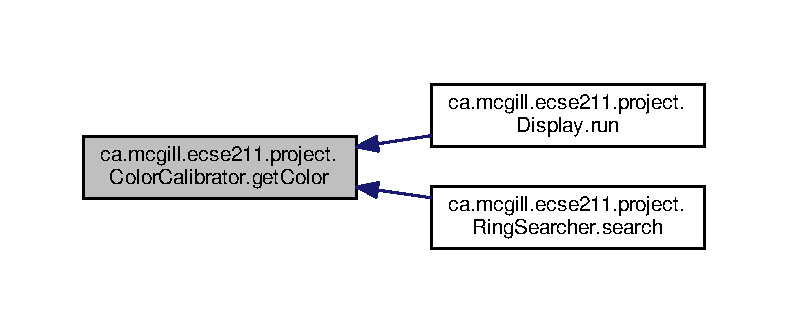
\includegraphics[width=350pt]{classca_1_1mcgill_1_1ecse211_1_1project_1_1_color_calibrator_a92e653a6a9f7a31cb7b6f9bc2e732133_icgraph}
\end{center}
\end{figure}
\mbox{\Hypertarget{classca_1_1mcgill_1_1ecse211_1_1project_1_1_color_calibrator_a1acf05f9523b2c0f329d4a7cbf1b9c47}\label{classca_1_1mcgill_1_1ecse211_1_1project_1_1_color_calibrator_a1acf05f9523b2c0f329d4a7cbf1b9c47}} 
\index{ca\+::mcgill\+::ecse211\+::project\+::\+Color\+Calibrator@{ca\+::mcgill\+::ecse211\+::project\+::\+Color\+Calibrator}!get\+Color@{get\+Color}}
\index{get\+Color@{get\+Color}!ca\+::mcgill\+::ecse211\+::project\+::\+Color\+Calibrator@{ca\+::mcgill\+::ecse211\+::project\+::\+Color\+Calibrator}}
\subsubsection{\texorpdfstring{get\+Color()}{getColor()}\hspace{0.1cm}{\footnotesize\ttfamily [2/2]}}
{\footnotesize\ttfamily static Color ca.\+mcgill.\+ecse211.\+project.\+Color\+Calibrator.\+get\+Color (\begin{DoxyParamCaption}{ }\end{DoxyParamCaption})\hspace{0.3cm}{\ttfamily [static]}}

This method gets the last color of the ring under the light sensor

\begin{DoxyReturn}{Returns}
current color detected by the light\+Sensor 
\end{DoxyReturn}


Definition at line 60 of file Color\+Calibrator.\+java.


\begin{DoxyCode}
60                                  \{
61     \textcolor{keywordflow}{if} (currentColor != null)
62       \textcolor{keywordflow}{return} currentColor;
63     \textcolor{keywordflow}{else}
64       \textcolor{keywordflow}{return} Color.Other;
65   \}
\end{DoxyCode}
\mbox{\Hypertarget{classca_1_1mcgill_1_1ecse211_1_1project_1_1_color_calibrator_acb1d9cef0739971dbe00cc16712be0fe}\label{classca_1_1mcgill_1_1ecse211_1_1project_1_1_color_calibrator_acb1d9cef0739971dbe00cc16712be0fe}} 
\index{ca\+::mcgill\+::ecse211\+::project\+::\+Color\+Calibrator@{ca\+::mcgill\+::ecse211\+::project\+::\+Color\+Calibrator}!get\+Get\+Color@{get\+Get\+Color}}
\index{get\+Get\+Color@{get\+Get\+Color}!ca\+::mcgill\+::ecse211\+::project\+::\+Color\+Calibrator@{ca\+::mcgill\+::ecse211\+::project\+::\+Color\+Calibrator}}
\subsubsection{\texorpdfstring{get\+Get\+Color()}{getGetColor()}}
{\footnotesize\ttfamily static Color ca.\+mcgill.\+ecse211.\+project.\+Color\+Calibrator.\+get\+Get\+Color (\begin{DoxyParamCaption}\item[{int}]{i }\end{DoxyParamCaption})\hspace{0.3cm}{\ttfamily [static]}}

This method match integer to corresponding color


\begin{DoxyParams}{Parameters}
{\em i} & an integer of \mbox{[}0,4\mbox{]} \\
\hline
\end{DoxyParams}
\begin{DoxyReturn}{Returns}
\+: cooresponding color of the integer 
\end{DoxyReturn}


Definition at line 128 of file Color\+Calibrator.\+java.


\begin{DoxyCode}
128                                          \{
129     Color c = Color.Other;
130     \textcolor{keywordflow}{switch} (i) \{
131       \textcolor{keywordflow}{case} 0:
132         c = Color.Other;
133         \textcolor{keywordflow}{break};
134       \textcolor{keywordflow}{case} 1:
135         c = Color.Blue;
136         \textcolor{keywordflow}{break};
137       \textcolor{keywordflow}{case} 2:
138         c = Color.Green;
139         \textcolor{keywordflow}{break};
140       \textcolor{keywordflow}{case} 3:
141         c = Color.Yellow;
142         \textcolor{keywordflow}{break};
143       \textcolor{keywordflow}{case} 4:
144         c = Color.Orange;
145         \textcolor{keywordflow}{break};
146     \}
147     \textcolor{keywordflow}{return} c;
148   \}
\end{DoxyCode}
Here is the caller graph for this function\+:\nopagebreak
\begin{figure}[H]
\begin{center}
\leavevmode
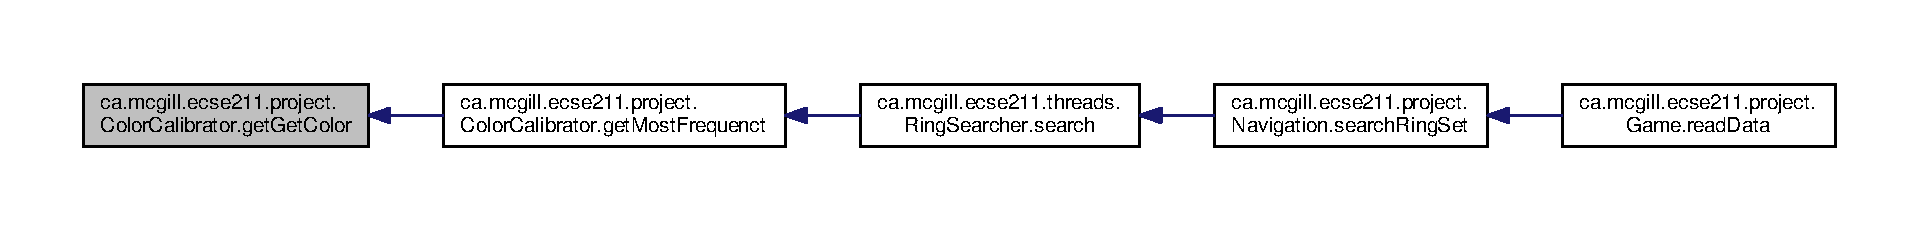
\includegraphics[width=350pt]{classca_1_1mcgill_1_1ecse211_1_1project_1_1_color_calibrator_acb1d9cef0739971dbe00cc16712be0fe_icgraph}
\end{center}
\end{figure}
\mbox{\Hypertarget{classca_1_1mcgill_1_1ecse211_1_1project_1_1_color_calibrator_a3d65927aaa2041f933dbdc19c3d2a412}\label{classca_1_1mcgill_1_1ecse211_1_1project_1_1_color_calibrator_a3d65927aaa2041f933dbdc19c3d2a412}} 
\index{ca\+::mcgill\+::ecse211\+::project\+::\+Color\+Calibrator@{ca\+::mcgill\+::ecse211\+::project\+::\+Color\+Calibrator}!get\+Most\+Frequenct@{get\+Most\+Frequenct}}
\index{get\+Most\+Frequenct@{get\+Most\+Frequenct}!ca\+::mcgill\+::ecse211\+::project\+::\+Color\+Calibrator@{ca\+::mcgill\+::ecse211\+::project\+::\+Color\+Calibrator}}
\subsubsection{\texorpdfstring{get\+Most\+Frequenct()}{getMostFrequenct()}}
{\footnotesize\ttfamily static Color ca.\+mcgill.\+ecse211.\+project.\+Color\+Calibrator.\+get\+Most\+Frequenct (\begin{DoxyParamCaption}{ }\end{DoxyParamCaption})\hspace{0.3cm}{\ttfamily [static]}}

This method returns the most frequent colour detected from multiple samples

\begin{DoxyReturn}{Returns}
most frequent colour detected 
\end{DoxyReturn}


Definition at line 96 of file Color\+Calibrator.\+java.


\begin{DoxyCode}
96                                          \{
97     Color c = Color.Other;
98     \textcolor{keywordtype}{int} frequency = colour\_frequency[0];
99     \textcolor{keywordflow}{for} (\textcolor{keywordtype}{int} i = 0; i < colour\_frequency.length; i++) \{
100       \textcolor{keywordflow}{if} (colour\_frequency[i] >= frequency) \{
101         frequency = colour\_frequency[i];
102         c = \hyperlink{classca_1_1mcgill_1_1ecse211_1_1project_1_1_color_calibrator_acb1d9cef0739971dbe00cc16712be0fe}{getGetColor}(i);
103       \}
104     \}
105     \textcolor{keywordflow}{if} (frequency == 0) \{
106       c = Color.Other;
107     \}
108     \hyperlink{classca_1_1mcgill_1_1ecse211_1_1project_1_1_color_calibrator_ab6148d75e3a105016580e90ed1ea9bc9}{resetFrequency}();
109     \textcolor{keywordflow}{return} c;
110   \}
\end{DoxyCode}
Here is the call graph for this function\+:\nopagebreak
\begin{figure}[H]
\begin{center}
\leavevmode
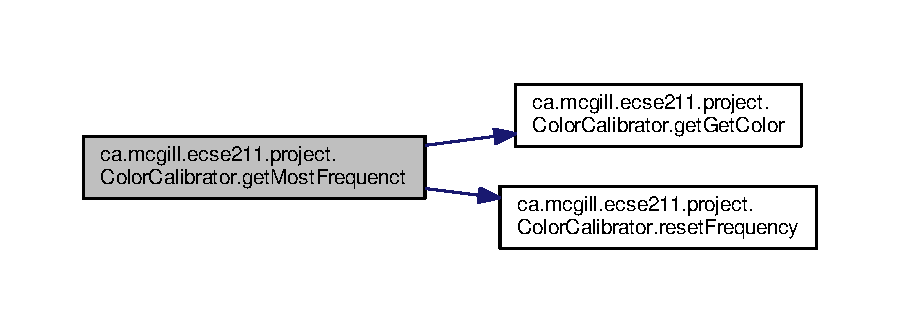
\includegraphics[width=350pt]{classca_1_1mcgill_1_1ecse211_1_1project_1_1_color_calibrator_a3d65927aaa2041f933dbdc19c3d2a412_cgraph}
\end{center}
\end{figure}
Here is the caller graph for this function\+:\nopagebreak
\begin{figure}[H]
\begin{center}
\leavevmode
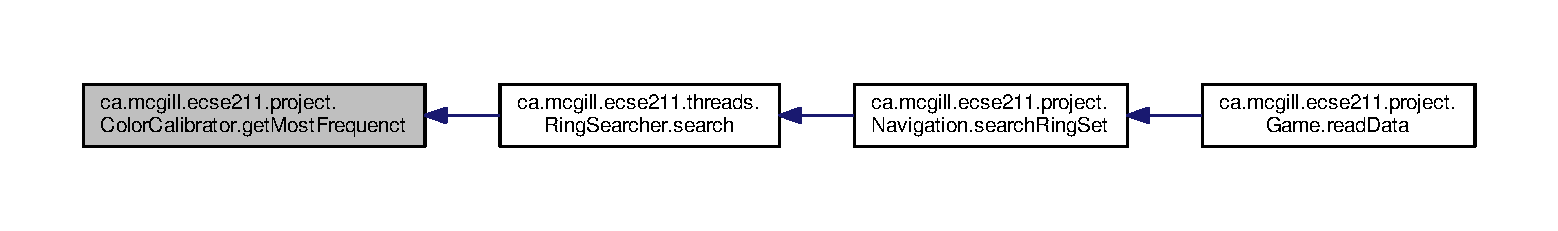
\includegraphics[width=350pt]{classca_1_1mcgill_1_1ecse211_1_1project_1_1_color_calibrator_a3d65927aaa2041f933dbdc19c3d2a412_icgraph}
\end{center}
\end{figure}
\mbox{\Hypertarget{classca_1_1mcgill_1_1ecse211_1_1project_1_1_color_calibrator_ab6148d75e3a105016580e90ed1ea9bc9}\label{classca_1_1mcgill_1_1ecse211_1_1project_1_1_color_calibrator_ab6148d75e3a105016580e90ed1ea9bc9}} 
\index{ca\+::mcgill\+::ecse211\+::project\+::\+Color\+Calibrator@{ca\+::mcgill\+::ecse211\+::project\+::\+Color\+Calibrator}!reset\+Frequency@{reset\+Frequency}}
\index{reset\+Frequency@{reset\+Frequency}!ca\+::mcgill\+::ecse211\+::project\+::\+Color\+Calibrator@{ca\+::mcgill\+::ecse211\+::project\+::\+Color\+Calibrator}}
\subsubsection{\texorpdfstring{reset\+Frequency()}{resetFrequency()}}
{\footnotesize\ttfamily static void ca.\+mcgill.\+ecse211.\+project.\+Color\+Calibrator.\+reset\+Frequency (\begin{DoxyParamCaption}{ }\end{DoxyParamCaption})\hspace{0.3cm}{\ttfamily [static]}}

This method resets the colour\+\_\+frequency array to 0 

Definition at line 116 of file Color\+Calibrator.\+java.


\begin{DoxyCode}
116                                       \{
117     \textcolor{keywordflow}{for} (\textcolor{keywordtype}{int} i = 0; i < colour\_frequency.length; i++) \{
118       colour\_frequency[i] = 0;
119     \}
120   \}
\end{DoxyCode}
Here is the caller graph for this function\+:\nopagebreak
\begin{figure}[H]
\begin{center}
\leavevmode
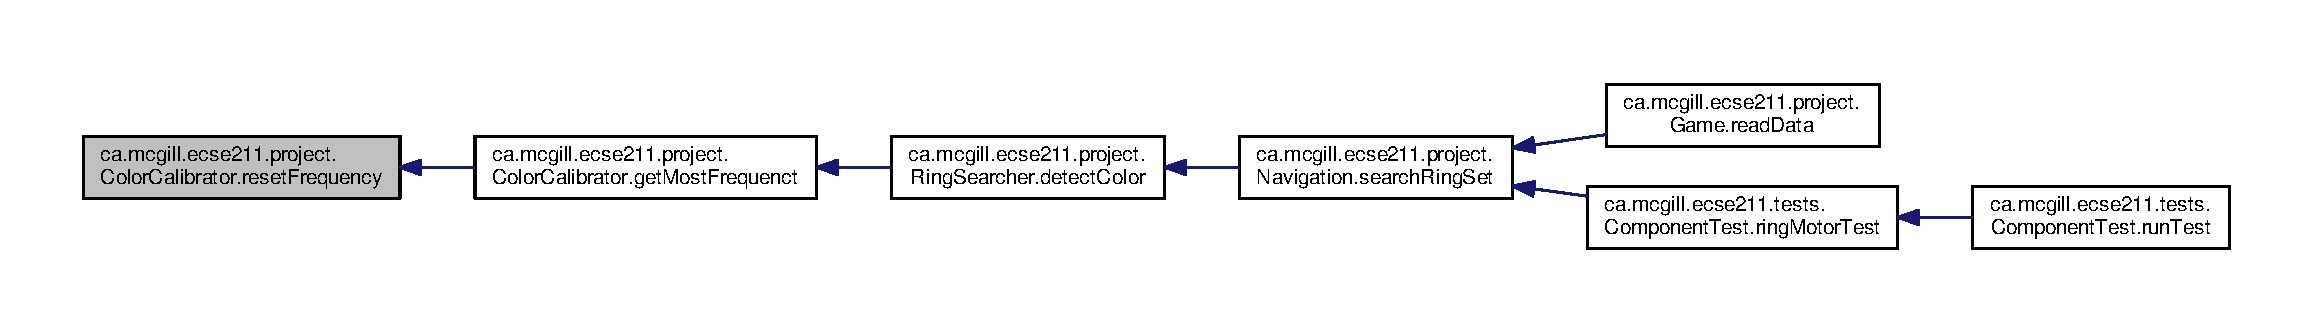
\includegraphics[width=350pt]{classca_1_1mcgill_1_1ecse211_1_1project_1_1_color_calibrator_ab6148d75e3a105016580e90ed1ea9bc9_icgraph}
\end{center}
\end{figure}
\mbox{\Hypertarget{classca_1_1mcgill_1_1ecse211_1_1project_1_1_color_calibrator_a40906193773ead0bfd582f188413c97a}\label{classca_1_1mcgill_1_1ecse211_1_1project_1_1_color_calibrator_a40906193773ead0bfd582f188413c97a}} 
\index{ca\+::mcgill\+::ecse211\+::project\+::\+Color\+Calibrator@{ca\+::mcgill\+::ecse211\+::project\+::\+Color\+Calibrator}!set\+Frequency@{set\+Frequency}}
\index{set\+Frequency@{set\+Frequency}!ca\+::mcgill\+::ecse211\+::project\+::\+Color\+Calibrator@{ca\+::mcgill\+::ecse211\+::project\+::\+Color\+Calibrator}}
\subsubsection{\texorpdfstring{set\+Frequency()}{setFrequency()}}
{\footnotesize\ttfamily static void ca.\+mcgill.\+ecse211.\+project.\+Color\+Calibrator.\+set\+Frequency (\begin{DoxyParamCaption}\item[{Color}]{c }\end{DoxyParamCaption})\hspace{0.3cm}{\ttfamily [static]}}

This method keeps track of how many of each colour were detected by increasing the count in the array


\begin{DoxyParams}{Parameters}
{\em c} & The Color detected by the light sensor \\
\hline
\end{DoxyParams}


Definition at line 73 of file Color\+Calibrator.\+java.


\begin{DoxyCode}
73                                            \{
74     \textcolor{keywordflow}{switch} (c) \{
75       \textcolor{keywordflow}{case} Blue:
76         colour\_frequency[1]++;
77         \textcolor{keywordflow}{break};
78       \textcolor{keywordflow}{case} Green:
79         colour\_frequency[2]++;
80         \textcolor{keywordflow}{break};
81       \textcolor{keywordflow}{case} Yellow:
82         colour\_frequency[3]++;
83         \textcolor{keywordflow}{break};
84       \textcolor{keywordflow}{case} Orange:
85         colour\_frequency[4]++;
86       \textcolor{keywordflow}{default}:
87         \textcolor{keywordflow}{break};
88     \}
89   \}
\end{DoxyCode}
Here is the caller graph for this function\+:\nopagebreak
\begin{figure}[H]
\begin{center}
\leavevmode
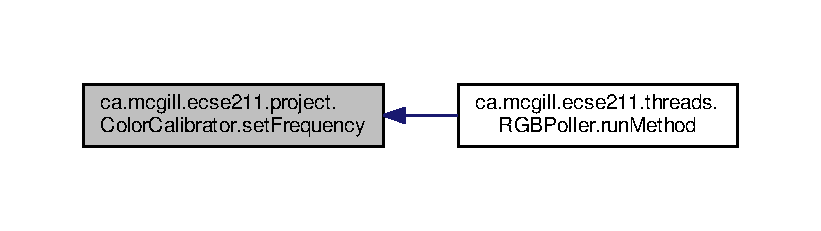
\includegraphics[width=350pt]{classca_1_1mcgill_1_1ecse211_1_1project_1_1_color_calibrator_a40906193773ead0bfd582f188413c97a_icgraph}
\end{center}
\end{figure}


The documentation for this class was generated from the following file\+:\begin{DoxyCompactItemize}
\item 
/home/ccc/\+Final\+Project/src/ca/mcgill/ecse211/project/\hyperlink{_color_calibrator_8java}{Color\+Calibrator.\+java}\end{DoxyCompactItemize}

\hypertarget{classca_1_1mcgill_1_1ecse211_1_1tests_1_1_component_test}{}\section{ca.\+mcgill.\+ecse211.\+tests.\+Component\+Test Class Reference}
\label{classca_1_1mcgill_1_1ecse211_1_1tests_1_1_component_test}\index{ca.\+mcgill.\+ecse211.\+tests.\+Component\+Test@{ca.\+mcgill.\+ecse211.\+tests.\+Component\+Test}}
\subsection*{Classes}
\begin{DoxyCompactItemize}
\item 
enum \hyperlink{enumca_1_1mcgill_1_1ecse211_1_1tests_1_1_component_test_1_1_type}{Type}
\end{DoxyCompactItemize}
\subsection*{Static Public Member Functions}
\begin{DoxyCompactItemize}
\item 
static void \hyperlink{classca_1_1mcgill_1_1ecse211_1_1tests_1_1_component_test_adcebcb6d834cb9c2461bccdd9831e74b}{run\+Test} (\hyperlink{enumca_1_1mcgill_1_1ecse211_1_1tests_1_1_component_test_1_1_type}{Type} type)
\item 
static void \hyperlink{classca_1_1mcgill_1_1ecse211_1_1tests_1_1_component_test_aa40592bb550b3526402faddbc0d890c7}{navigation\+Test} ()  throws Odometer\+Exceptions 
\item 
static void \hyperlink{classca_1_1mcgill_1_1ecse211_1_1tests_1_1_component_test_ad11712dd74c5c64e84cd71186a59a087}{localization\+Test} ()  throws Odometer\+Exceptions 
\item 
static void \hyperlink{classca_1_1mcgill_1_1ecse211_1_1tests_1_1_component_test_a05cd9d95458b11ed57ca001a28fffa7c}{ultrasonic\+Sensor\+Test} ()
\item 
static void \hyperlink{classca_1_1mcgill_1_1ecse211_1_1tests_1_1_component_test_a3e8288f482b3806a0f3c4668951f3e36}{light\+Sensor\+Test} ()
\item 
static void \hyperlink{classca_1_1mcgill_1_1ecse211_1_1tests_1_1_component_test_a3782f843fd251f8bb14be0cb1d291dd5}{Ring\+Motor\+Test} ()  throws Odometer\+Exceptions 
\end{DoxyCompactItemize}


\subsection{Detailed Description}


Definition at line 8 of file Component\+Test.\+java.



\subsection{Member Function Documentation}
\mbox{\Hypertarget{classca_1_1mcgill_1_1ecse211_1_1tests_1_1_component_test_a3e8288f482b3806a0f3c4668951f3e36}\label{classca_1_1mcgill_1_1ecse211_1_1tests_1_1_component_test_a3e8288f482b3806a0f3c4668951f3e36}} 
\index{ca\+::mcgill\+::ecse211\+::tests\+::\+Component\+Test@{ca\+::mcgill\+::ecse211\+::tests\+::\+Component\+Test}!light\+Sensor\+Test@{light\+Sensor\+Test}}
\index{light\+Sensor\+Test@{light\+Sensor\+Test}!ca\+::mcgill\+::ecse211\+::tests\+::\+Component\+Test@{ca\+::mcgill\+::ecse211\+::tests\+::\+Component\+Test}}
\subsubsection{\texorpdfstring{light\+Sensor\+Test()}{lightSensorTest()}}
{\footnotesize\ttfamily static void ca.\+mcgill.\+ecse211.\+tests.\+Component\+Test.\+light\+Sensor\+Test (\begin{DoxyParamCaption}{ }\end{DoxyParamCaption})\hspace{0.3cm}{\ttfamily [static]}}

Test for light\+Sensor 

Definition at line 50 of file Component\+Test.\+java.

\mbox{\Hypertarget{classca_1_1mcgill_1_1ecse211_1_1tests_1_1_component_test_ad11712dd74c5c64e84cd71186a59a087}\label{classca_1_1mcgill_1_1ecse211_1_1tests_1_1_component_test_ad11712dd74c5c64e84cd71186a59a087}} 
\index{ca\+::mcgill\+::ecse211\+::tests\+::\+Component\+Test@{ca\+::mcgill\+::ecse211\+::tests\+::\+Component\+Test}!localization\+Test@{localization\+Test}}
\index{localization\+Test@{localization\+Test}!ca\+::mcgill\+::ecse211\+::tests\+::\+Component\+Test@{ca\+::mcgill\+::ecse211\+::tests\+::\+Component\+Test}}
\subsubsection{\texorpdfstring{localization\+Test()}{localizationTest()}}
{\footnotesize\ttfamily static void ca.\+mcgill.\+ecse211.\+tests.\+Component\+Test.\+localization\+Test (\begin{DoxyParamCaption}{ }\end{DoxyParamCaption}) throws \hyperlink{classca_1_1mcgill_1_1ecse211_1_1odometer_1_1_odometer_exceptions}{Odometer\+Exceptions}\hspace{0.3cm}{\ttfamily [static]}}

Test for localization\+Test 
\begin{DoxyExceptions}{Exceptions}
{\em Odometer\+Exceptions} & \\
\hline
\end{DoxyExceptions}


Definition at line 36 of file Component\+Test.\+java.

\mbox{\Hypertarget{classca_1_1mcgill_1_1ecse211_1_1tests_1_1_component_test_aa40592bb550b3526402faddbc0d890c7}\label{classca_1_1mcgill_1_1ecse211_1_1tests_1_1_component_test_aa40592bb550b3526402faddbc0d890c7}} 
\index{ca\+::mcgill\+::ecse211\+::tests\+::\+Component\+Test@{ca\+::mcgill\+::ecse211\+::tests\+::\+Component\+Test}!navigation\+Test@{navigation\+Test}}
\index{navigation\+Test@{navigation\+Test}!ca\+::mcgill\+::ecse211\+::tests\+::\+Component\+Test@{ca\+::mcgill\+::ecse211\+::tests\+::\+Component\+Test}}
\subsubsection{\texorpdfstring{navigation\+Test()}{navigationTest()}}
{\footnotesize\ttfamily static void ca.\+mcgill.\+ecse211.\+tests.\+Component\+Test.\+navigation\+Test (\begin{DoxyParamCaption}{ }\end{DoxyParamCaption}) throws \hyperlink{classca_1_1mcgill_1_1ecse211_1_1odometer_1_1_odometer_exceptions}{Odometer\+Exceptions}\hspace{0.3cm}{\ttfamily [static]}}

Test for Navigation 
\begin{DoxyExceptions}{Exceptions}
{\em Odometer\+Exceptions} & \\
\hline
\end{DoxyExceptions}


Definition at line 26 of file Component\+Test.\+java.

Here is the call graph for this function\+:
\nopagebreak
\begin{figure}[H]
\begin{center}
\leavevmode
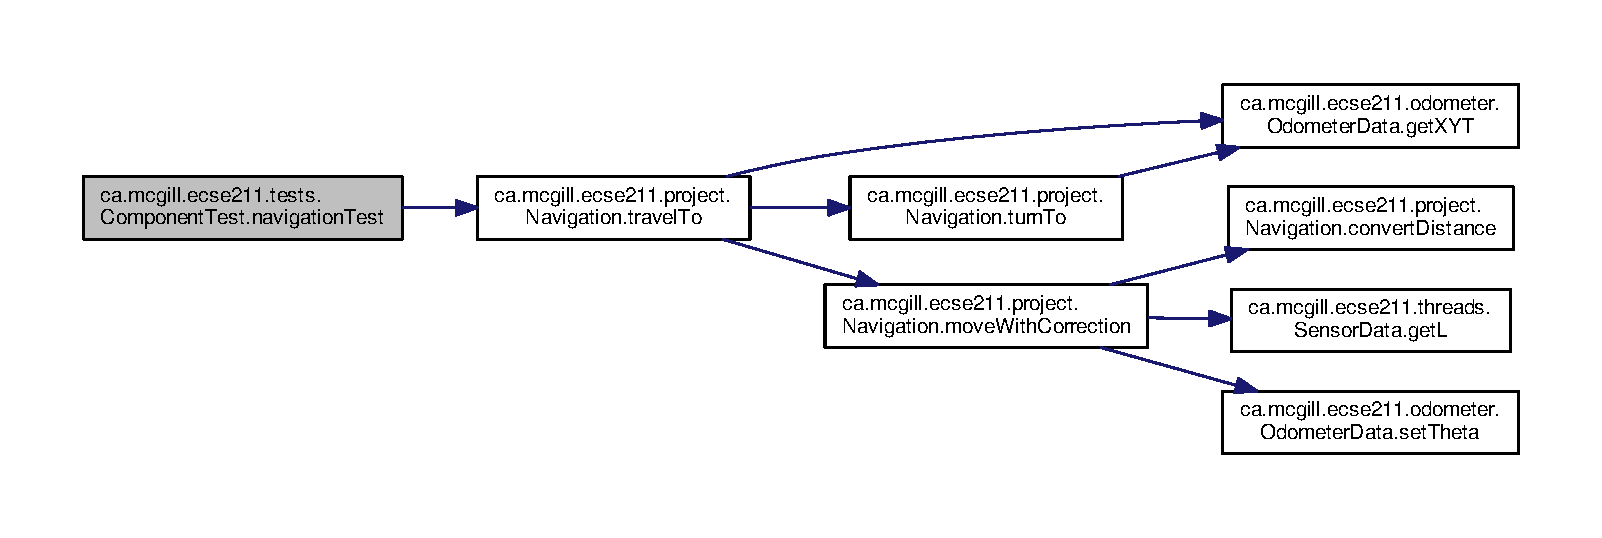
\includegraphics[width=350pt]{classca_1_1mcgill_1_1ecse211_1_1tests_1_1_component_test_aa40592bb550b3526402faddbc0d890c7_cgraph}
\end{center}
\end{figure}
\mbox{\Hypertarget{classca_1_1mcgill_1_1ecse211_1_1tests_1_1_component_test_a3782f843fd251f8bb14be0cb1d291dd5}\label{classca_1_1mcgill_1_1ecse211_1_1tests_1_1_component_test_a3782f843fd251f8bb14be0cb1d291dd5}} 
\index{ca\+::mcgill\+::ecse211\+::tests\+::\+Component\+Test@{ca\+::mcgill\+::ecse211\+::tests\+::\+Component\+Test}!Ring\+Motor\+Test@{Ring\+Motor\+Test}}
\index{Ring\+Motor\+Test@{Ring\+Motor\+Test}!ca\+::mcgill\+::ecse211\+::tests\+::\+Component\+Test@{ca\+::mcgill\+::ecse211\+::tests\+::\+Component\+Test}}
\subsubsection{\texorpdfstring{Ring\+Motor\+Test()}{RingMotorTest()}}
{\footnotesize\ttfamily static void ca.\+mcgill.\+ecse211.\+tests.\+Component\+Test.\+Ring\+Motor\+Test (\begin{DoxyParamCaption}{ }\end{DoxyParamCaption}) throws \hyperlink{classca_1_1mcgill_1_1ecse211_1_1odometer_1_1_odometer_exceptions}{Odometer\+Exceptions}\hspace{0.3cm}{\ttfamily [static]}}

Test for ring detection 
\begin{DoxyExceptions}{Exceptions}
{\em Odometer\+Exceptions} & \\
\hline
\end{DoxyExceptions}


Definition at line 58 of file Component\+Test.\+java.

Here is the call graph for this function\+:
\nopagebreak
\begin{figure}[H]
\begin{center}
\leavevmode
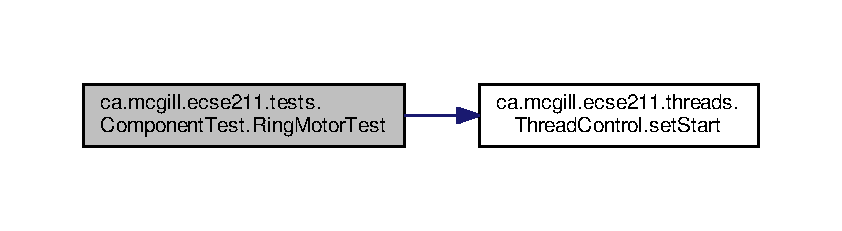
\includegraphics[width=350pt]{classca_1_1mcgill_1_1ecse211_1_1tests_1_1_component_test_a3782f843fd251f8bb14be0cb1d291dd5_cgraph}
\end{center}
\end{figure}
Here is the caller graph for this function\+:
\nopagebreak
\begin{figure}[H]
\begin{center}
\leavevmode
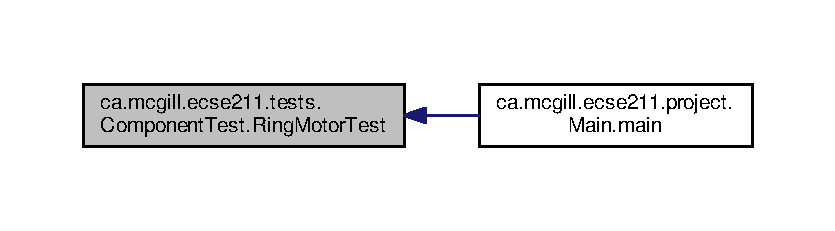
\includegraphics[width=350pt]{classca_1_1mcgill_1_1ecse211_1_1tests_1_1_component_test_a3782f843fd251f8bb14be0cb1d291dd5_icgraph}
\end{center}
\end{figure}
\mbox{\Hypertarget{classca_1_1mcgill_1_1ecse211_1_1tests_1_1_component_test_adcebcb6d834cb9c2461bccdd9831e74b}\label{classca_1_1mcgill_1_1ecse211_1_1tests_1_1_component_test_adcebcb6d834cb9c2461bccdd9831e74b}} 
\index{ca\+::mcgill\+::ecse211\+::tests\+::\+Component\+Test@{ca\+::mcgill\+::ecse211\+::tests\+::\+Component\+Test}!run\+Test@{run\+Test}}
\index{run\+Test@{run\+Test}!ca\+::mcgill\+::ecse211\+::tests\+::\+Component\+Test@{ca\+::mcgill\+::ecse211\+::tests\+::\+Component\+Test}}
\subsubsection{\texorpdfstring{run\+Test()}{runTest()}}
{\footnotesize\ttfamily static void ca.\+mcgill.\+ecse211.\+tests.\+Component\+Test.\+run\+Test (\begin{DoxyParamCaption}\item[{\hyperlink{enumca_1_1mcgill_1_1ecse211_1_1tests_1_1_component_test_1_1_type}{Type}}]{type }\end{DoxyParamCaption})\hspace{0.3cm}{\ttfamily [static]}}

This method selects test for each individual components of the design


\begin{DoxyParams}{Parameters}
{\em type} & \\
\hline
\end{DoxyParams}


Definition at line 18 of file Component\+Test.\+java.

\mbox{\Hypertarget{classca_1_1mcgill_1_1ecse211_1_1tests_1_1_component_test_a05cd9d95458b11ed57ca001a28fffa7c}\label{classca_1_1mcgill_1_1ecse211_1_1tests_1_1_component_test_a05cd9d95458b11ed57ca001a28fffa7c}} 
\index{ca\+::mcgill\+::ecse211\+::tests\+::\+Component\+Test@{ca\+::mcgill\+::ecse211\+::tests\+::\+Component\+Test}!ultrasonic\+Sensor\+Test@{ultrasonic\+Sensor\+Test}}
\index{ultrasonic\+Sensor\+Test@{ultrasonic\+Sensor\+Test}!ca\+::mcgill\+::ecse211\+::tests\+::\+Component\+Test@{ca\+::mcgill\+::ecse211\+::tests\+::\+Component\+Test}}
\subsubsection{\texorpdfstring{ultrasonic\+Sensor\+Test()}{ultrasonicSensorTest()}}
{\footnotesize\ttfamily static void ca.\+mcgill.\+ecse211.\+tests.\+Component\+Test.\+ultrasonic\+Sensor\+Test (\begin{DoxyParamCaption}{ }\end{DoxyParamCaption})\hspace{0.3cm}{\ttfamily [static]}}

Test for Ultrasonic\+Sensor 

Definition at line 43 of file Component\+Test.\+java.



The documentation for this class was generated from the following file\+:\begin{DoxyCompactItemize}
\item 
/home/ccc/\+Final\+Project/src/ca/mcgill/ecse211/tests/Component\+Test.\+java\end{DoxyCompactItemize}

\hypertarget{classca_1_1mcgill_1_1ecse211_1_1project_1_1_display}{}\section{ca.\+mcgill.\+ecse211.\+project.\+Display Class Reference}
\label{classca_1_1mcgill_1_1ecse211_1_1project_1_1_display}\index{ca.\+mcgill.\+ecse211.\+project.\+Display@{ca.\+mcgill.\+ecse211.\+project.\+Display}}


Inheritance diagram for ca.\+mcgill.\+ecse211.\+project.\+Display\+:\nopagebreak
\begin{figure}[H]
\begin{center}
\leavevmode
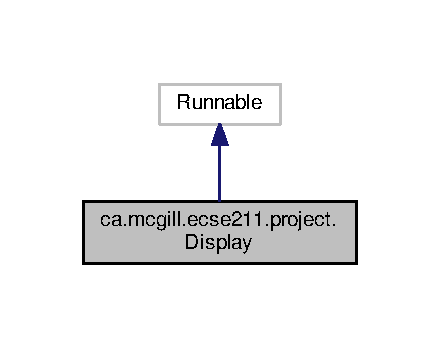
\includegraphics[width=211pt]{classca_1_1mcgill_1_1ecse211_1_1project_1_1_display__inherit__graph}
\end{center}
\end{figure}


Collaboration diagram for ca.\+mcgill.\+ecse211.\+project.\+Display\+:\nopagebreak
\begin{figure}[H]
\begin{center}
\leavevmode
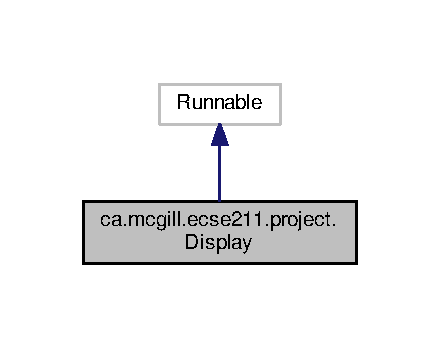
\includegraphics[width=211pt]{classca_1_1mcgill_1_1ecse211_1_1project_1_1_display__coll__graph}
\end{center}
\end{figure}
\subsection*{Public Member Functions}
\begin{DoxyCompactItemize}
\item 
\hyperlink{classca_1_1mcgill_1_1ecse211_1_1project_1_1_display_af0970123ca090749bfb2f5b9f478c01d}{Display} (Text\+L\+CD lcd)  throws Odometer\+Exceptions 
\item 
\hyperlink{classca_1_1mcgill_1_1ecse211_1_1project_1_1_display_a690cd91bcc8024950c2b8e3b2613c801}{Display} (Text\+L\+CD lcd, long timeout)  throws Odometer\+Exceptions 
\item 
void \hyperlink{classca_1_1mcgill_1_1ecse211_1_1project_1_1_display_ab508a8bc2b738499bec2c432a814cba5}{run} ()
\end{DoxyCompactItemize}


\subsection{Detailed Description}
This class is used to display the content of the odometer variables (x, y, Theta)

\begin{DoxyAuthor}{Author}
Caspar Cedro 

Percy Chen 

Patrick Erath 

Anssam Ghezala 

Susan Matuszewski 

Kamy Moussavi Kafi 
\end{DoxyAuthor}


Definition at line 19 of file Display.\+java.



\subsection{Constructor \& Destructor Documentation}
\mbox{\Hypertarget{classca_1_1mcgill_1_1ecse211_1_1project_1_1_display_af0970123ca090749bfb2f5b9f478c01d}\label{classca_1_1mcgill_1_1ecse211_1_1project_1_1_display_af0970123ca090749bfb2f5b9f478c01d}} 
\index{ca\+::mcgill\+::ecse211\+::project\+::\+Display@{ca\+::mcgill\+::ecse211\+::project\+::\+Display}!Display@{Display}}
\index{Display@{Display}!ca\+::mcgill\+::ecse211\+::project\+::\+Display@{ca\+::mcgill\+::ecse211\+::project\+::\+Display}}
\subsubsection{\texorpdfstring{Display()}{Display()}\hspace{0.1cm}{\footnotesize\ttfamily [1/2]}}
{\footnotesize\ttfamily ca.\+mcgill.\+ecse211.\+project.\+Display.\+Display (\begin{DoxyParamCaption}\item[{Text\+L\+CD}]{lcd }\end{DoxyParamCaption}) throws \hyperlink{classca_1_1mcgill_1_1ecse211_1_1odometer_1_1_odometer_exceptions}{Odometer\+Exceptions}}

This is the class constructor for a display object that controls an E\+V3 brick display


\begin{DoxyParams}{Parameters}
{\em lcd} & A Text\+L\+CD object instance to control \\
\hline
\end{DoxyParams}

\begin{DoxyExceptions}{Exceptions}
{\em Odometer\+Exceptions} & \\
\hline
\end{DoxyExceptions}


Definition at line 35 of file Display.\+java.


\begin{DoxyCode}
35                                                         \{
36     this.odo = Odometer.\hyperlink{classca_1_1mcgill_1_1ecse211_1_1odometer_1_1_odometer_a99171f11e34dea918fa9dd069d721439}{getOdometer}();
37     this.sensdata = SensorData.\hyperlink{classca_1_1mcgill_1_1ecse211_1_1threads_1_1_sensor_data_a8260aba53b4474ca1275e4ce26157977}{getSensorData}();
38     this.lcd = lcd;
39   \}
\end{DoxyCode}
Here is the call graph for this function\+:\nopagebreak
\begin{figure}[H]
\begin{center}
\leavevmode
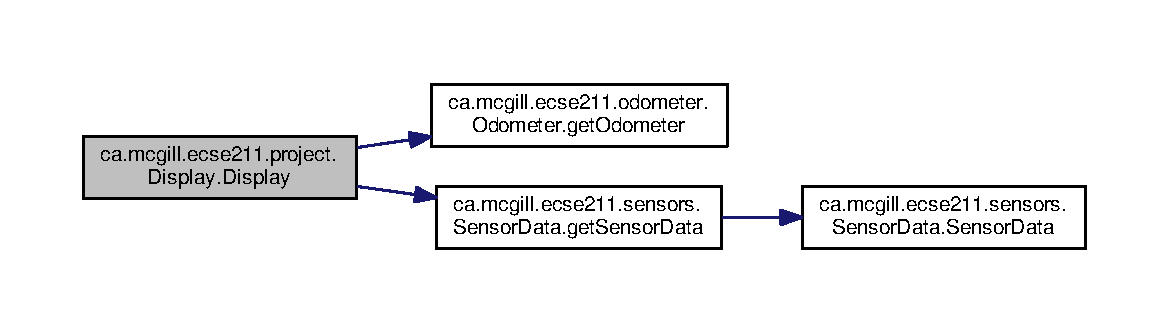
\includegraphics[width=350pt]{classca_1_1mcgill_1_1ecse211_1_1project_1_1_display_af0970123ca090749bfb2f5b9f478c01d_cgraph}
\end{center}
\end{figure}
\mbox{\Hypertarget{classca_1_1mcgill_1_1ecse211_1_1project_1_1_display_a690cd91bcc8024950c2b8e3b2613c801}\label{classca_1_1mcgill_1_1ecse211_1_1project_1_1_display_a690cd91bcc8024950c2b8e3b2613c801}} 
\index{ca\+::mcgill\+::ecse211\+::project\+::\+Display@{ca\+::mcgill\+::ecse211\+::project\+::\+Display}!Display@{Display}}
\index{Display@{Display}!ca\+::mcgill\+::ecse211\+::project\+::\+Display@{ca\+::mcgill\+::ecse211\+::project\+::\+Display}}
\subsubsection{\texorpdfstring{Display()}{Display()}\hspace{0.1cm}{\footnotesize\ttfamily [2/2]}}
{\footnotesize\ttfamily ca.\+mcgill.\+ecse211.\+project.\+Display.\+Display (\begin{DoxyParamCaption}\item[{Text\+L\+CD}]{lcd,  }\item[{long}]{timeout }\end{DoxyParamCaption}) throws \hyperlink{classca_1_1mcgill_1_1ecse211_1_1odometer_1_1_odometer_exceptions}{Odometer\+Exceptions}}

This is the overloaded class constructor for a display object


\begin{DoxyParams}{Parameters}
{\em lcd} & A Text\+L\+CD object instance to control \\
\hline
{\em timeout} & A duration of time to update the display for \\
\hline
\end{DoxyParams}

\begin{DoxyExceptions}{Exceptions}
{\em Odometer\+Exceptions} & \\
\hline
\end{DoxyExceptions}


Definition at line 48 of file Display.\+java.


\begin{DoxyCode}
48                                                                       \{
49     odo = Odometer.\hyperlink{classca_1_1mcgill_1_1ecse211_1_1odometer_1_1_odometer_a99171f11e34dea918fa9dd069d721439}{getOdometer}();
50     this.timeout = timeout;
51     this.lcd = lcd;
52   \}
\end{DoxyCode}
Here is the call graph for this function\+:\nopagebreak
\begin{figure}[H]
\begin{center}
\leavevmode
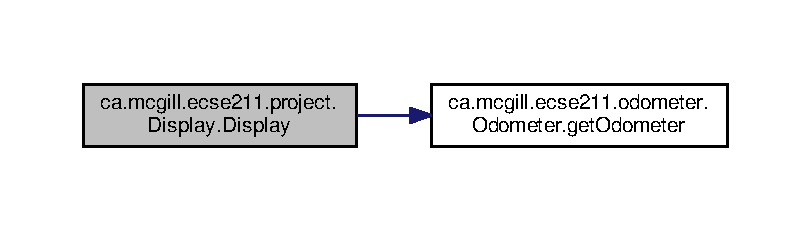
\includegraphics[width=350pt]{classca_1_1mcgill_1_1ecse211_1_1project_1_1_display_a690cd91bcc8024950c2b8e3b2613c801_cgraph}
\end{center}
\end{figure}


\subsection{Member Function Documentation}
\mbox{\Hypertarget{classca_1_1mcgill_1_1ecse211_1_1project_1_1_display_ab508a8bc2b738499bec2c432a814cba5}\label{classca_1_1mcgill_1_1ecse211_1_1project_1_1_display_ab508a8bc2b738499bec2c432a814cba5}} 
\index{ca\+::mcgill\+::ecse211\+::project\+::\+Display@{ca\+::mcgill\+::ecse211\+::project\+::\+Display}!run@{run}}
\index{run@{run}!ca\+::mcgill\+::ecse211\+::project\+::\+Display@{ca\+::mcgill\+::ecse211\+::project\+::\+Display}}
\subsubsection{\texorpdfstring{run()}{run()}}
{\footnotesize\ttfamily void ca.\+mcgill.\+ecse211.\+project.\+Display.\+run (\begin{DoxyParamCaption}{ }\end{DoxyParamCaption})}

This method is called when the \hyperlink{classca_1_1mcgill_1_1ecse211_1_1project_1_1_display}{Display} thread is started. 

Definition at line 57 of file Display.\+java.


\begin{DoxyCode}
57                     \{
58     lcd.clear();
59 
60     \textcolor{keywordtype}{long} updateStart, updateEnd;
61 
62     \textcolor{keywordtype}{long} tStart = System.currentTimeMillis();
63 
64     \textcolor{keywordflow}{do} \{
65       updateStart = System.currentTimeMillis();
66 
67       \textcolor{comment}{// Retrieve x, y and Theta information}
68       position = odo.\hyperlink{classca_1_1mcgill_1_1ecse211_1_1odometer_1_1_odometer_data_a8f40f0264c68f0cbed4fff1723ae7863}{getXYT}();
69       rgb = sensdata.\hyperlink{classca_1_1mcgill_1_1ecse211_1_1threads_1_1_sensor_data_a76313564e284f5cdb66aefce4e595f3b}{getRGB}();
70 
71       \textcolor{comment}{// Print x,y, and theta information}
72       DecimalFormat numberFormat = \textcolor{keyword}{new} DecimalFormat(\textcolor{stringliteral}{"######0.00"});
73       \textcolor{comment}{// The last two parameters to lcd.drawString denote the x and y coordinate to draw at.}
74    \textcolor{comment}{//   lcd.drawString("X: " + numberFormat.format(position[0]), 0, 0);}
75    \textcolor{comment}{//   lcd.drawString("Y: " + numberFormat.format(position[1]), 0, 1);}
76   \textcolor{comment}{//    lcd.drawString("T: " + numberFormat.format(position[2]), 0, 2);}
77 \textcolor{comment}{//      lcd.drawString("LL: " + numberFormat.format(sensdata.getL()[0]), 0, 3);}
78 \textcolor{comment}{//      lcd.drawString("LR: " + numberFormat.format(sensdata.getL()[1]), 0, 4);}
79 \textcolor{comment}{//      lcd.drawString("D: " + numberFormat.format(sensdata.getD()), 0, 5);}
80 
81       lcd.drawString(String.format(\textcolor{stringliteral}{"(R: %d G: %d B: %d)"}, (\textcolor{keywordtype}{int}) rgb[0], (\textcolor{keywordtype}{int}) rgb[1], (\textcolor{keywordtype}{int}) rgb[2]),
82           0, 4);
83 \textcolor{comment}{//      if (ColorCalibrator.getColor((int) rgb[0], (int) rgb[1],}
84 \textcolor{comment}{//          (int) rgb[2]) != ColorCalibrator.Color.Other) \{}
85 \textcolor{comment}{//        lcd.drawString("Object Detected", 0, 5);}
86 \textcolor{comment}{//      \} else \{}
87 \textcolor{comment}{//        // Draw whitespace on our display}
88 \textcolor{comment}{//        lcd.drawString("                   ", 0, 5);}
89 \textcolor{comment}{//      \}}
90 
91       lcd.drawString(String.format(\textcolor{stringliteral}{"%1$-10s"}, ColorCalibrator.getColor().toString()), 0, 6);
92       lcd.drawString(\textcolor{stringliteral}{"A:"} + numberFormat.format(sensdata.\hyperlink{classca_1_1mcgill_1_1ecse211_1_1threads_1_1_sensor_data_acc8f6cc56f39c8ea6b812cd8b135eca6}{getA}()), 0, 7);
93 
94 \textcolor{comment}{//       lcd.drawString(String.format("(r: %d", (int)rgb[0]), 0, 3);}
95 \textcolor{comment}{//       lcd.drawString(String.format("(g: %d", (int)rgb[1]), 0, 4);}
96 \textcolor{comment}{//       lcd.drawString(String.format("(b: %d", (int)rgb[2]), 0, 5);}
97 
98       \textcolor{comment}{// This ensures that the data is updated only once every period}
99       updateEnd = System.currentTimeMillis();
100       \textcolor{keywordflow}{if} (updateEnd - updateStart < DISPLAY\_PERIOD) \{
101         \textcolor{keywordflow}{try} \{
102           Thread.sleep(DISPLAY\_PERIOD - (updateEnd - updateStart));
103         \} \textcolor{keywordflow}{catch} (InterruptedException e) \{
104           e.printStackTrace();
105         \}
106       \}
107     \} \textcolor{keywordflow}{while} ((updateEnd - tStart) <= timeout);
108   \}
\end{DoxyCode}
Here is the call graph for this function\+:\nopagebreak
\begin{figure}[H]
\begin{center}
\leavevmode
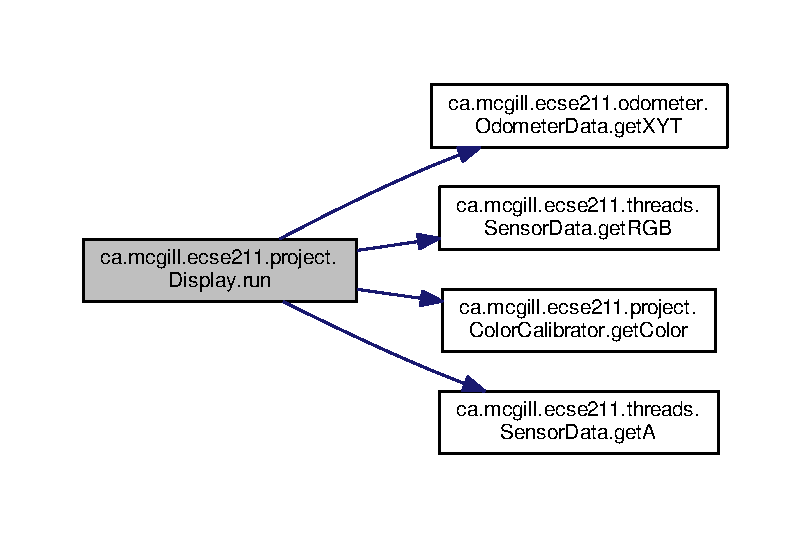
\includegraphics[width=350pt]{classca_1_1mcgill_1_1ecse211_1_1project_1_1_display_ab508a8bc2b738499bec2c432a814cba5_cgraph}
\end{center}
\end{figure}


The documentation for this class was generated from the following file\+:\begin{DoxyCompactItemize}
\item 
/home/ccc/\+Final\+Project/src/ca/mcgill/ecse211/project/\hyperlink{_display_8java}{Display.\+java}\end{DoxyCompactItemize}

\hypertarget{classca_1_1mcgill_1_1ecse211_1_1project_1_1_game}{}\section{ca.\+mcgill.\+ecse211.\+project.\+Game Class Reference}
\label{classca_1_1mcgill_1_1ecse211_1_1project_1_1_game}\index{ca.\+mcgill.\+ecse211.\+project.\+Game@{ca.\+mcgill.\+ecse211.\+project.\+Game}}


Collaboration diagram for ca.\+mcgill.\+ecse211.\+project.\+Game\+:
\nopagebreak
\begin{figure}[H]
\begin{center}
\leavevmode
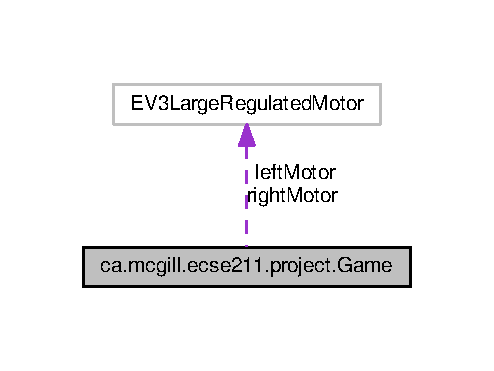
\includegraphics[width=350pt]{classca_1_1mcgill_1_1ecse211_1_1project_1_1_game__coll__graph}
\end{center}
\end{figure}
\subsection*{Static Public Member Functions}
\begin{DoxyCompactItemize}
\item 
static void \hyperlink{classca_1_1mcgill_1_1ecse211_1_1project_1_1_game_a1bcbd1c19309c65a6887ae19bde66765}{preparation} ()  throws Odometer\+Exceptions 
\item 
static synchronized void \hyperlink{classca_1_1mcgill_1_1ecse211_1_1project_1_1_game_aff9431d27d78c8b228f468d8ad889a9a}{read\+Data} ()
\item 
static synchronized void \hyperlink{classca_1_1mcgill_1_1ecse211_1_1project_1_1_game_a790740a4ed299c9b985401ea8c4d5010}{run\+Game} ()  throws Odometer\+Exceptions 
\end{DoxyCompactItemize}
\subsection*{Static Public Attributes}
\begin{DoxyCompactItemize}
\item 
static final E\+V3\+Large\+Regulated\+Motor \hyperlink{classca_1_1mcgill_1_1ecse211_1_1project_1_1_game_a40f6d5a8c70b88bf89b2171a02d2813f}{left\+Motor}
\item 
static final E\+V3\+Large\+Regulated\+Motor \hyperlink{classca_1_1mcgill_1_1ecse211_1_1project_1_1_game_a637614c1eb769dcdb09d897c66e453a2}{right\+Motor}
\item 
static final E\+V3\+Large\+Regulated\+Motor \hyperlink{classca_1_1mcgill_1_1ecse211_1_1project_1_1_game_a37d42c1d3b40b8eaa429866e37cd86c7}{storage\+Motor}
\item 
static final E\+V3\+Medium\+Regulated\+Motor \hyperlink{classca_1_1mcgill_1_1ecse211_1_1project_1_1_game_ad3c828a8e12ad3eaab01d2d846a3716f}{rod\+Motor}
\item 
static final double \hyperlink{classca_1_1mcgill_1_1ecse211_1_1project_1_1_game_a9a7a353789ddffcb938827410318b4fe}{T\+I\+LE} = 30.\+48
\item 
static final double \hyperlink{classca_1_1mcgill_1_1ecse211_1_1project_1_1_game_a206492a827a716e6c606dc817cb4ff4d}{W\+H\+E\+E\+L\+\_\+\+R\+AD} = 2.\+15
\item 
static final double \hyperlink{classca_1_1mcgill_1_1ecse211_1_1project_1_1_game_aa445d106d7fba82e78405e64087916b6}{T\+R\+A\+CK} = 11.\+5
\item 
static final double \hyperlink{classca_1_1mcgill_1_1ecse211_1_1project_1_1_game_a7eb34dc64ead0f2c0db2367f773ae94c}{S\+E\+N\+\_\+\+D\+IS} = 4.\+4
\end{DoxyCompactItemize}


\subsection{Detailed Description}
This class implements the main starting point for the Search and Localize lab

\begin{DoxyAuthor}{Author}
Caspar Cedro 

Percy Chen 

Patrick Erath 

Anssam Ghezala 

Susan Matuszewski 

Kamy Moussavi Kafi 
\end{DoxyAuthor}


Definition at line 33 of file Game.\+java.



\subsection{Member Function Documentation}
\mbox{\Hypertarget{classca_1_1mcgill_1_1ecse211_1_1project_1_1_game_a1bcbd1c19309c65a6887ae19bde66765}\label{classca_1_1mcgill_1_1ecse211_1_1project_1_1_game_a1bcbd1c19309c65a6887ae19bde66765}} 
\index{ca\+::mcgill\+::ecse211\+::project\+::\+Game@{ca\+::mcgill\+::ecse211\+::project\+::\+Game}!preparation@{preparation}}
\index{preparation@{preparation}!ca\+::mcgill\+::ecse211\+::project\+::\+Game@{ca\+::mcgill\+::ecse211\+::project\+::\+Game}}
\subsubsection{\texorpdfstring{preparation()}{preparation()}}
{\footnotesize\ttfamily static void ca.\+mcgill.\+ecse211.\+project.\+Game.\+preparation (\begin{DoxyParamCaption}{ }\end{DoxyParamCaption}) throws \hyperlink{classca_1_1mcgill_1_1ecse211_1_1odometer_1_1_odometer_exceptions}{Odometer\+Exceptions}\hspace{0.3cm}{\ttfamily [static]}}

Prepare for the game\+: starting thread, read all arguments


\begin{DoxyExceptions}{Exceptions}
{\em Odometer\+Exceptions} & \\
\hline
\end{DoxyExceptions}


Definition at line 90 of file Game.\+java.

Here is the call graph for this function\+:
\nopagebreak
\begin{figure}[H]
\begin{center}
\leavevmode
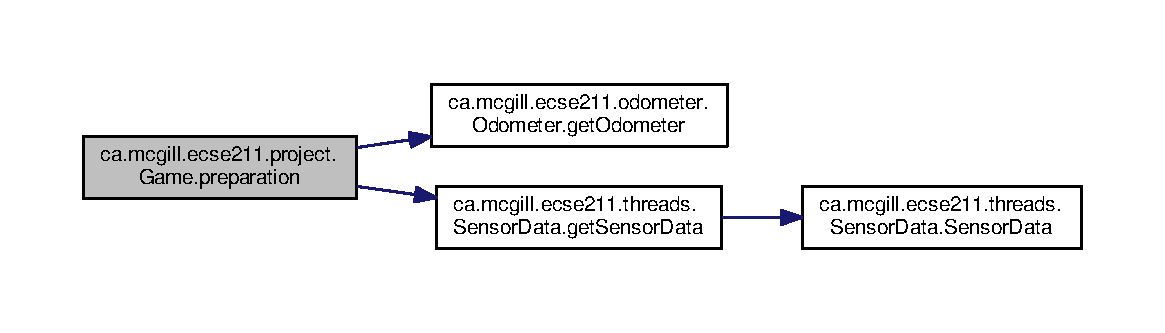
\includegraphics[width=350pt]{classca_1_1mcgill_1_1ecse211_1_1project_1_1_game_a1bcbd1c19309c65a6887ae19bde66765_cgraph}
\end{center}
\end{figure}
Here is the caller graph for this function\+:
\nopagebreak
\begin{figure}[H]
\begin{center}
\leavevmode
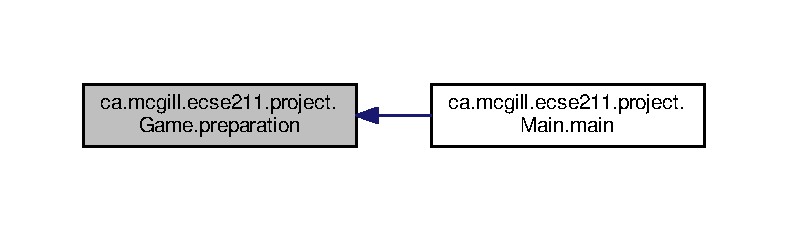
\includegraphics[width=350pt]{classca_1_1mcgill_1_1ecse211_1_1project_1_1_game_a1bcbd1c19309c65a6887ae19bde66765_icgraph}
\end{center}
\end{figure}
\mbox{\Hypertarget{classca_1_1mcgill_1_1ecse211_1_1project_1_1_game_aff9431d27d78c8b228f468d8ad889a9a}\label{classca_1_1mcgill_1_1ecse211_1_1project_1_1_game_aff9431d27d78c8b228f468d8ad889a9a}} 
\index{ca\+::mcgill\+::ecse211\+::project\+::\+Game@{ca\+::mcgill\+::ecse211\+::project\+::\+Game}!read\+Data@{read\+Data}}
\index{read\+Data@{read\+Data}!ca\+::mcgill\+::ecse211\+::project\+::\+Game@{ca\+::mcgill\+::ecse211\+::project\+::\+Game}}
\subsubsection{\texorpdfstring{read\+Data()}{readData()}}
{\footnotesize\ttfamily static synchronized void ca.\+mcgill.\+ecse211.\+project.\+Game.\+read\+Data (\begin{DoxyParamCaption}{ }\end{DoxyParamCaption})\hspace{0.3cm}{\ttfamily [static]}}

Read data from the wifi class (using another thread) 

Definition at line 153 of file Game.\+java.

Here is the caller graph for this function\+:
\nopagebreak
\begin{figure}[H]
\begin{center}
\leavevmode
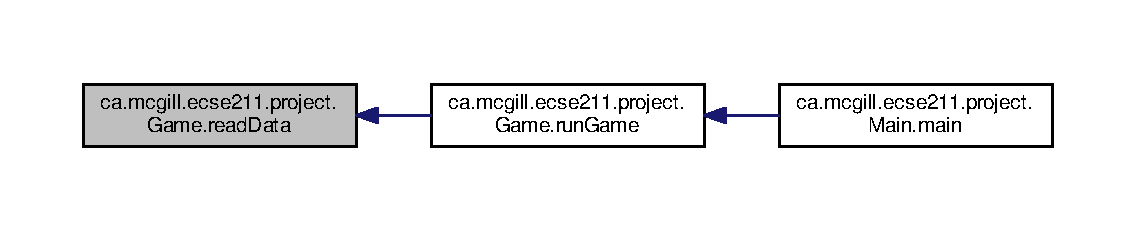
\includegraphics[width=350pt]{classca_1_1mcgill_1_1ecse211_1_1project_1_1_game_aff9431d27d78c8b228f468d8ad889a9a_icgraph}
\end{center}
\end{figure}
\mbox{\Hypertarget{classca_1_1mcgill_1_1ecse211_1_1project_1_1_game_a790740a4ed299c9b985401ea8c4d5010}\label{classca_1_1mcgill_1_1ecse211_1_1project_1_1_game_a790740a4ed299c9b985401ea8c4d5010}} 
\index{ca\+::mcgill\+::ecse211\+::project\+::\+Game@{ca\+::mcgill\+::ecse211\+::project\+::\+Game}!run\+Game@{run\+Game}}
\index{run\+Game@{run\+Game}!ca\+::mcgill\+::ecse211\+::project\+::\+Game@{ca\+::mcgill\+::ecse211\+::project\+::\+Game}}
\subsubsection{\texorpdfstring{run\+Game()}{runGame()}}
{\footnotesize\ttfamily static synchronized void ca.\+mcgill.\+ecse211.\+project.\+Game.\+run\+Game (\begin{DoxyParamCaption}{ }\end{DoxyParamCaption}) throws \hyperlink{classca_1_1mcgill_1_1ecse211_1_1odometer_1_1_odometer_exceptions}{Odometer\+Exceptions}\hspace{0.3cm}{\ttfamily [static]}}

This method contains main logic for the game plays


\begin{DoxyExceptions}{Exceptions}
{\em Odometer\+Exceptions} & \\
\hline
\end{DoxyExceptions}


Definition at line 162 of file Game.\+java.

Here is the call graph for this function\+:
\nopagebreak
\begin{figure}[H]
\begin{center}
\leavevmode
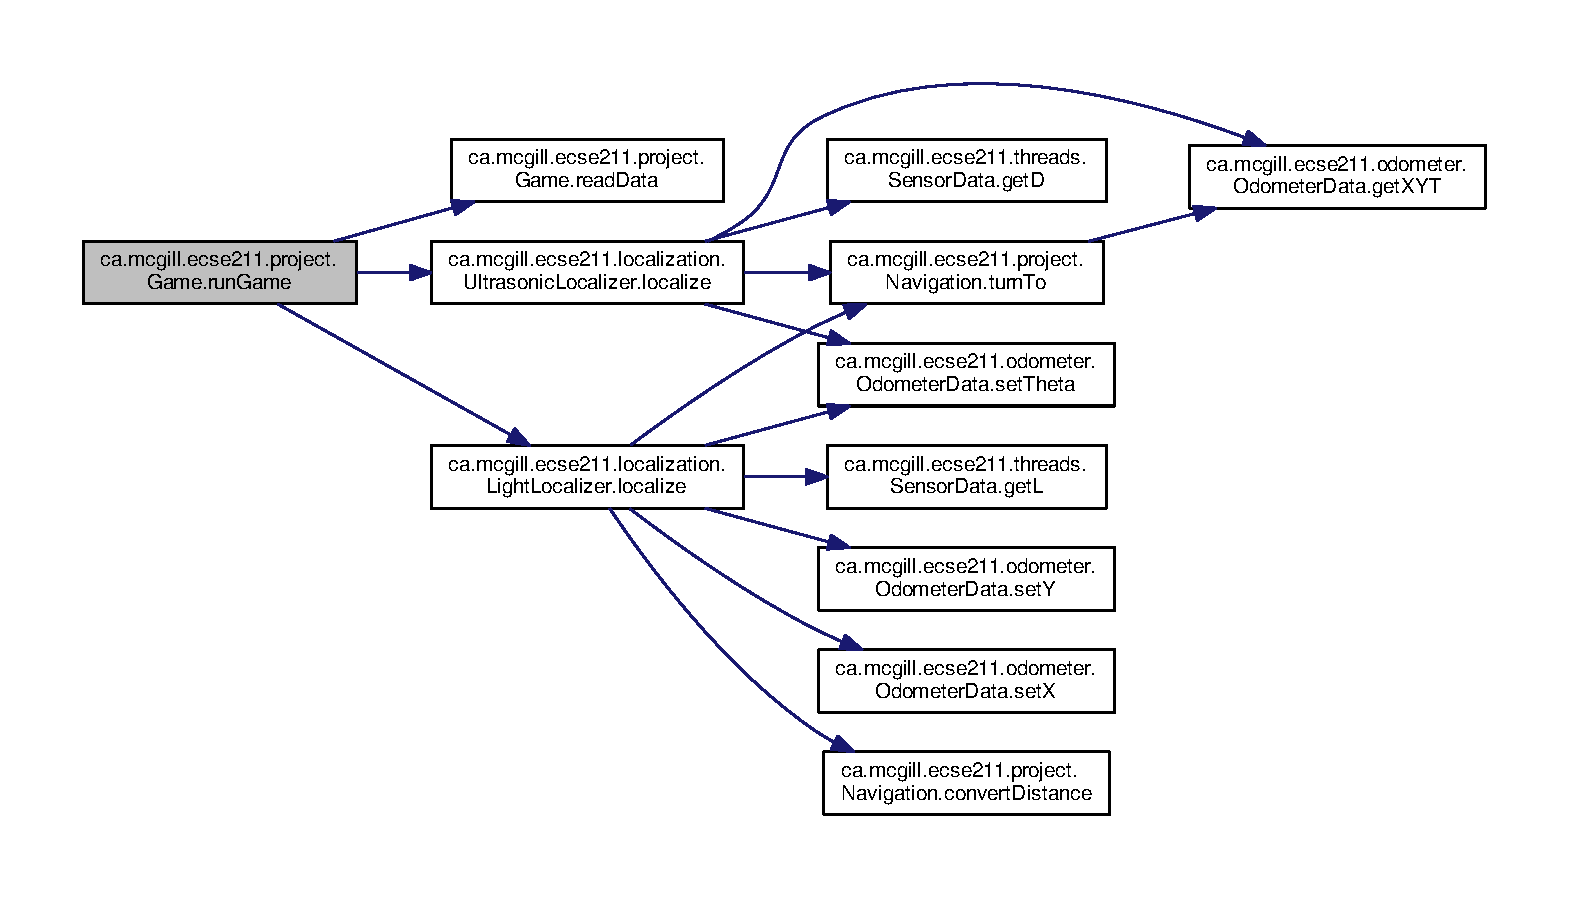
\includegraphics[width=350pt]{classca_1_1mcgill_1_1ecse211_1_1project_1_1_game_a790740a4ed299c9b985401ea8c4d5010_cgraph}
\end{center}
\end{figure}
Here is the caller graph for this function\+:
\nopagebreak
\begin{figure}[H]
\begin{center}
\leavevmode
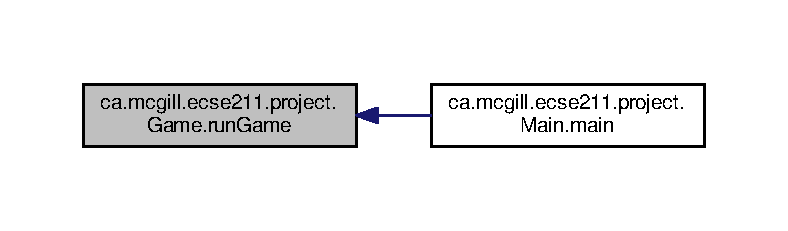
\includegraphics[width=350pt]{classca_1_1mcgill_1_1ecse211_1_1project_1_1_game_a790740a4ed299c9b985401ea8c4d5010_icgraph}
\end{center}
\end{figure}


\subsection{Member Data Documentation}
\mbox{\Hypertarget{classca_1_1mcgill_1_1ecse211_1_1project_1_1_game_a40f6d5a8c70b88bf89b2171a02d2813f}\label{classca_1_1mcgill_1_1ecse211_1_1project_1_1_game_a40f6d5a8c70b88bf89b2171a02d2813f}} 
\index{ca\+::mcgill\+::ecse211\+::project\+::\+Game@{ca\+::mcgill\+::ecse211\+::project\+::\+Game}!left\+Motor@{left\+Motor}}
\index{left\+Motor@{left\+Motor}!ca\+::mcgill\+::ecse211\+::project\+::\+Game@{ca\+::mcgill\+::ecse211\+::project\+::\+Game}}
\subsubsection{\texorpdfstring{left\+Motor}{leftMotor}}
{\footnotesize\ttfamily final E\+V3\+Large\+Regulated\+Motor ca.\+mcgill.\+ecse211.\+project.\+Game.\+left\+Motor\hspace{0.3cm}{\ttfamily [static]}}

{\bfseries Initial value\+:}
\begin{DoxyCode}
=
      \textcolor{keyword}{new} EV3LargeRegulatedMotor(LocalEV3.get().getPort(\textcolor{stringliteral}{"A"}))
\end{DoxyCode}
Motor object instance that allows control of the left motor connected to port A 

Definition at line 42 of file Game.\+java.

\mbox{\Hypertarget{classca_1_1mcgill_1_1ecse211_1_1project_1_1_game_a637614c1eb769dcdb09d897c66e453a2}\label{classca_1_1mcgill_1_1ecse211_1_1project_1_1_game_a637614c1eb769dcdb09d897c66e453a2}} 
\index{ca\+::mcgill\+::ecse211\+::project\+::\+Game@{ca\+::mcgill\+::ecse211\+::project\+::\+Game}!right\+Motor@{right\+Motor}}
\index{right\+Motor@{right\+Motor}!ca\+::mcgill\+::ecse211\+::project\+::\+Game@{ca\+::mcgill\+::ecse211\+::project\+::\+Game}}
\subsubsection{\texorpdfstring{right\+Motor}{rightMotor}}
{\footnotesize\ttfamily final E\+V3\+Large\+Regulated\+Motor ca.\+mcgill.\+ecse211.\+project.\+Game.\+right\+Motor\hspace{0.3cm}{\ttfamily [static]}}

{\bfseries Initial value\+:}
\begin{DoxyCode}
=
      \textcolor{keyword}{new} EV3LargeRegulatedMotor(LocalEV3.get().getPort(\textcolor{stringliteral}{"D"}))
\end{DoxyCode}
Motor object instance that allows control of the right motor connected to port D 

Definition at line 48 of file Game.\+java.

\mbox{\Hypertarget{classca_1_1mcgill_1_1ecse211_1_1project_1_1_game_ad3c828a8e12ad3eaab01d2d846a3716f}\label{classca_1_1mcgill_1_1ecse211_1_1project_1_1_game_ad3c828a8e12ad3eaab01d2d846a3716f}} 
\index{ca\+::mcgill\+::ecse211\+::project\+::\+Game@{ca\+::mcgill\+::ecse211\+::project\+::\+Game}!rod\+Motor@{rod\+Motor}}
\index{rod\+Motor@{rod\+Motor}!ca\+::mcgill\+::ecse211\+::project\+::\+Game@{ca\+::mcgill\+::ecse211\+::project\+::\+Game}}
\subsubsection{\texorpdfstring{rod\+Motor}{rodMotor}}
{\footnotesize\ttfamily final E\+V3\+Medium\+Regulated\+Motor ca.\+mcgill.\+ecse211.\+project.\+Game.\+rod\+Motor\hspace{0.3cm}{\ttfamily [static]}}

{\bfseries Initial value\+:}
\begin{DoxyCode}
=
      \textcolor{keyword}{new} EV3MediumRegulatedMotor(LocalEV3.get().getPort(\textcolor{stringliteral}{"B"}))
\end{DoxyCode}
Motor object instance taht allows control of the motor on the rod for collecting rings 

Definition at line 60 of file Game.\+java.

\mbox{\Hypertarget{classca_1_1mcgill_1_1ecse211_1_1project_1_1_game_a7eb34dc64ead0f2c0db2367f773ae94c}\label{classca_1_1mcgill_1_1ecse211_1_1project_1_1_game_a7eb34dc64ead0f2c0db2367f773ae94c}} 
\index{ca\+::mcgill\+::ecse211\+::project\+::\+Game@{ca\+::mcgill\+::ecse211\+::project\+::\+Game}!S\+E\+N\+\_\+\+D\+IS@{S\+E\+N\+\_\+\+D\+IS}}
\index{S\+E\+N\+\_\+\+D\+IS@{S\+E\+N\+\_\+\+D\+IS}!ca\+::mcgill\+::ecse211\+::project\+::\+Game@{ca\+::mcgill\+::ecse211\+::project\+::\+Game}}
\subsubsection{\texorpdfstring{S\+E\+N\+\_\+\+D\+IS}{SEN\_DIS}}
{\footnotesize\ttfamily final double ca.\+mcgill.\+ecse211.\+project.\+Game.\+S\+E\+N\+\_\+\+D\+IS = 4.\+4\hspace{0.3cm}{\ttfamily [static]}}

The distance between light sensor and the center of the robot in cm 

Definition at line 81 of file Game.\+java.

\mbox{\Hypertarget{classca_1_1mcgill_1_1ecse211_1_1project_1_1_game_a37d42c1d3b40b8eaa429866e37cd86c7}\label{classca_1_1mcgill_1_1ecse211_1_1project_1_1_game_a37d42c1d3b40b8eaa429866e37cd86c7}} 
\index{ca\+::mcgill\+::ecse211\+::project\+::\+Game@{ca\+::mcgill\+::ecse211\+::project\+::\+Game}!storage\+Motor@{storage\+Motor}}
\index{storage\+Motor@{storage\+Motor}!ca\+::mcgill\+::ecse211\+::project\+::\+Game@{ca\+::mcgill\+::ecse211\+::project\+::\+Game}}
\subsubsection{\texorpdfstring{storage\+Motor}{storageMotor}}
{\footnotesize\ttfamily final E\+V3\+Large\+Regulated\+Motor ca.\+mcgill.\+ecse211.\+project.\+Game.\+storage\+Motor\hspace{0.3cm}{\ttfamily [static]}}

{\bfseries Initial value\+:}
\begin{DoxyCode}
=
      \textcolor{keyword}{new} EV3LargeRegulatedMotor(LocalEV3.get().getPort(\textcolor{stringliteral}{"C"}))
\end{DoxyCode}
Motor object instance that allows control of the motor on storage rod 

Definition at line 54 of file Game.\+java.

\mbox{\Hypertarget{classca_1_1mcgill_1_1ecse211_1_1project_1_1_game_a9a7a353789ddffcb938827410318b4fe}\label{classca_1_1mcgill_1_1ecse211_1_1project_1_1_game_a9a7a353789ddffcb938827410318b4fe}} 
\index{ca\+::mcgill\+::ecse211\+::project\+::\+Game@{ca\+::mcgill\+::ecse211\+::project\+::\+Game}!T\+I\+LE@{T\+I\+LE}}
\index{T\+I\+LE@{T\+I\+LE}!ca\+::mcgill\+::ecse211\+::project\+::\+Game@{ca\+::mcgill\+::ecse211\+::project\+::\+Game}}
\subsubsection{\texorpdfstring{T\+I\+LE}{TILE}}
{\footnotesize\ttfamily final double ca.\+mcgill.\+ecse211.\+project.\+Game.\+T\+I\+LE = 30.\+48\hspace{0.3cm}{\ttfamily [static]}}

length of the tile 

Definition at line 65 of file Game.\+java.

\mbox{\Hypertarget{classca_1_1mcgill_1_1ecse211_1_1project_1_1_game_aa445d106d7fba82e78405e64087916b6}\label{classca_1_1mcgill_1_1ecse211_1_1project_1_1_game_aa445d106d7fba82e78405e64087916b6}} 
\index{ca\+::mcgill\+::ecse211\+::project\+::\+Game@{ca\+::mcgill\+::ecse211\+::project\+::\+Game}!T\+R\+A\+CK@{T\+R\+A\+CK}}
\index{T\+R\+A\+CK@{T\+R\+A\+CK}!ca\+::mcgill\+::ecse211\+::project\+::\+Game@{ca\+::mcgill\+::ecse211\+::project\+::\+Game}}
\subsubsection{\texorpdfstring{T\+R\+A\+CK}{TRACK}}
{\footnotesize\ttfamily final double ca.\+mcgill.\+ecse211.\+project.\+Game.\+T\+R\+A\+CK = 11.\+5\hspace{0.3cm}{\ttfamily [static]}}

This variable denotes the track distance between the center of the wheels in cm (measured and adjusted based on trial and error). 

Definition at line 76 of file Game.\+java.

\mbox{\Hypertarget{classca_1_1mcgill_1_1ecse211_1_1project_1_1_game_a206492a827a716e6c606dc817cb4ff4d}\label{classca_1_1mcgill_1_1ecse211_1_1project_1_1_game_a206492a827a716e6c606dc817cb4ff4d}} 
\index{ca\+::mcgill\+::ecse211\+::project\+::\+Game@{ca\+::mcgill\+::ecse211\+::project\+::\+Game}!W\+H\+E\+E\+L\+\_\+\+R\+AD@{W\+H\+E\+E\+L\+\_\+\+R\+AD}}
\index{W\+H\+E\+E\+L\+\_\+\+R\+AD@{W\+H\+E\+E\+L\+\_\+\+R\+AD}!ca\+::mcgill\+::ecse211\+::project\+::\+Game@{ca\+::mcgill\+::ecse211\+::project\+::\+Game}}
\subsubsection{\texorpdfstring{W\+H\+E\+E\+L\+\_\+\+R\+AD}{WHEEL\_RAD}}
{\footnotesize\ttfamily final double ca.\+mcgill.\+ecse211.\+project.\+Game.\+W\+H\+E\+E\+L\+\_\+\+R\+AD = 2.\+15\hspace{0.3cm}{\ttfamily [static]}}

This variable denotes the radius of our wheels in cm. 

Definition at line 70 of file Game.\+java.



The documentation for this class was generated from the following file\+:\begin{DoxyCompactItemize}
\item 
/home/ccc/\+Final\+Project/src/ca/mcgill/ecse211/project/Game.\+java\end{DoxyCompactItemize}

\hypertarget{classca_1_1mcgill_1_1ecse211_1_1project_1_1_game_parameters}{}\section{ca.\+mcgill.\+ecse211.\+project.\+Game\+Parameters Class Reference}
\label{classca_1_1mcgill_1_1ecse211_1_1project_1_1_game_parameters}\index{ca.\+mcgill.\+ecse211.\+project.\+Game\+Parameters@{ca.\+mcgill.\+ecse211.\+project.\+Game\+Parameters}}
\subsection*{Static Public Attributes}
\begin{DoxyCompactItemize}
\item 
static int \mbox{[}$\,$\mbox{]} \hyperlink{classca_1_1mcgill_1_1ecse211_1_1project_1_1_game_parameters_aae8c69151bc01acce692b9119323bb46}{SC} = \{-\/1, -\/1\}
\item 
static int \mbox{[}$\,$\mbox{]} \hyperlink{classca_1_1mcgill_1_1ecse211_1_1project_1_1_game_parameters_aec739d9ebcbd75db6a77ec288ff974cf}{Grid\+\_\+\+LL} = \{0, 0\}
\item 
static int \mbox{[}$\,$\mbox{]} \hyperlink{classca_1_1mcgill_1_1ecse211_1_1project_1_1_game_parameters_ab79c9c891076d29cbe5ac053f617c381}{Grid\+\_\+\+UR} = \{15, 9\}
\item 
static int \hyperlink{classca_1_1mcgill_1_1ecse211_1_1project_1_1_game_parameters_a5a299e93e098c89d12be1072947d3bcb}{TR} = -\/1
\item 
static int \hyperlink{classca_1_1mcgill_1_1ecse211_1_1project_1_1_game_parameters_a15bc3c24f73d1ad29b6fe7fd9e1ef0e6}{Player\+Team\+Number} = -\/1
\item 
static int \hyperlink{classca_1_1mcgill_1_1ecse211_1_1project_1_1_game_parameters_a51c899921677197f960f39e6ed42c780}{Red\+Team} = -\/1
\item 
static int \hyperlink{classca_1_1mcgill_1_1ecse211_1_1project_1_1_game_parameters_aca550f5067892ceeb8f44ede61bbc90e}{Green\+Team} = -\/1
\item 
static int \hyperlink{classca_1_1mcgill_1_1ecse211_1_1project_1_1_game_parameters_acf0dce5eb9dc754248f0c3de997d2809}{Red\+Corner} = -\/1
\item 
static int \hyperlink{classca_1_1mcgill_1_1ecse211_1_1project_1_1_game_parameters_a7fe7f10f96800fbd5f2331e3aa608b66}{Green\+Corner} = -\/1
\item 
static int \mbox{[}$\,$\mbox{]} \hyperlink{classca_1_1mcgill_1_1ecse211_1_1project_1_1_game_parameters_ae3eb3c87467d3a7760cd619a96379a9e}{Red\+\_\+\+LL} = \{0, 5\}
\item 
static int \mbox{[}$\,$\mbox{]} \hyperlink{classca_1_1mcgill_1_1ecse211_1_1project_1_1_game_parameters_a81ddd789119962c32fe6d7f9cce4f240}{Red\+\_\+\+UR} = \{4, 9\}
\item 
static int \mbox{[}$\,$\mbox{]} \hyperlink{classca_1_1mcgill_1_1ecse211_1_1project_1_1_game_parameters_a24e38b735e194403bf2b9877241969c1}{Green\+\_\+\+LL} = \{10, 0\}
\item 
static int \mbox{[}$\,$\mbox{]} \hyperlink{classca_1_1mcgill_1_1ecse211_1_1project_1_1_game_parameters_aedb13ca3822f3581bdffd464891b1494}{Green\+\_\+\+UR} = \{15, 4\}
\item 
static int \mbox{[}$\,$\mbox{]} \hyperlink{classca_1_1mcgill_1_1ecse211_1_1project_1_1_game_parameters_a8695da7f04954ea1513082740fd2d57f}{B\+R\+R\+\_\+\+LL} = \{4, 7\}
\item 
static int \mbox{[}$\,$\mbox{]} \hyperlink{classca_1_1mcgill_1_1ecse211_1_1project_1_1_game_parameters_a720d0ae20fc2466e7b77fda14bf374f3}{B\+R\+R\+\_\+\+UR} = \{6, 8\}
\item 
static int \mbox{[}$\,$\mbox{]} \hyperlink{classca_1_1mcgill_1_1ecse211_1_1project_1_1_game_parameters_ae6824f16adf03173062767f99d46b6e0}{B\+R\+G\+\_\+\+LL} = \{10, 3\}
\item 
static int \mbox{[}$\,$\mbox{]} \hyperlink{classca_1_1mcgill_1_1ecse211_1_1project_1_1_game_parameters_a644c339e7b0f11c5780f9c7de34e1e07}{B\+R\+G\+\_\+\+UR} = \{11, 5\}
\item 
static int \mbox{[}$\,$\mbox{]} \hyperlink{classca_1_1mcgill_1_1ecse211_1_1project_1_1_game_parameters_ac642730053a35524ce70866289ca10b9}{T\+R\+\_\+\+LL} = \{7, 6\}
\item 
static int \mbox{[}$\,$\mbox{]} \hyperlink{classca_1_1mcgill_1_1ecse211_1_1project_1_1_game_parameters_a45c465e9f0b53a4e752a398036be13f5}{T\+R\+\_\+\+UR} = \{8, 7\}
\item 
static int \mbox{[}$\,$\mbox{]} \hyperlink{classca_1_1mcgill_1_1ecse211_1_1project_1_1_game_parameters_a0fefeecefd65deabea205bd9d628bf76}{T\+G\+\_\+\+LL} = \{13, 7\}
\item 
static int \mbox{[}$\,$\mbox{]} \hyperlink{classca_1_1mcgill_1_1ecse211_1_1project_1_1_game_parameters_aa8220987d04f322d9480db7cc073ffd2}{T\+G\+\_\+\+UR} = \{14, 8\}
\end{DoxyCompactItemize}


\subsection{Detailed Description}


Definition at line 3 of file Game\+Parameters.\+java.



\subsection{Member Data Documentation}
\mbox{\Hypertarget{classca_1_1mcgill_1_1ecse211_1_1project_1_1_game_parameters_ae6824f16adf03173062767f99d46b6e0}\label{classca_1_1mcgill_1_1ecse211_1_1project_1_1_game_parameters_ae6824f16adf03173062767f99d46b6e0}} 
\index{ca\+::mcgill\+::ecse211\+::project\+::\+Game\+Parameters@{ca\+::mcgill\+::ecse211\+::project\+::\+Game\+Parameters}!B\+R\+G\+\_\+\+LL@{B\+R\+G\+\_\+\+LL}}
\index{B\+R\+G\+\_\+\+LL@{B\+R\+G\+\_\+\+LL}!ca\+::mcgill\+::ecse211\+::project\+::\+Game\+Parameters@{ca\+::mcgill\+::ecse211\+::project\+::\+Game\+Parameters}}
\subsubsection{\texorpdfstring{B\+R\+G\+\_\+\+LL}{BRG\_LL}}
{\footnotesize\ttfamily int \mbox{[}$\,$\mbox{]} ca.\+mcgill.\+ecse211.\+project.\+Game\+Parameters.\+B\+R\+G\+\_\+\+LL = \{10, 3\}\hspace{0.3cm}{\ttfamily [static]}}

This variable stores the lower left hand corner of the green tunnel footprint. \mbox{[}0\mbox{]} = x coordinate, \mbox{[}1\mbox{]} = y coordinate min B\+R\+G\+\_\+\+UR\mbox{[}0\mbox{]} -\/ B\+R\+G\+\_\+\+LL\mbox{[}0\mbox{]} = 1 max B\+R\+G\+\_\+\+UR\mbox{[}0\mbox{]} -\/ B\+R\+G\+\_\+\+LL\mbox{[}0\mbox{]} = 2 min B\+R\+G\+\_\+\+UR\mbox{[}1\mbox{]} -\/ B\+R\+G\+\_\+\+LL\mbox{[}1\mbox{]} = 1 max B\+R\+G\+\_\+\+UR\mbox{[}1\mbox{]} -\/ B\+R\+G\+\_\+\+LL\mbox{[}1\mbox{]} = 2 

Definition at line 118 of file Game\+Parameters.\+java.

\mbox{\Hypertarget{classca_1_1mcgill_1_1ecse211_1_1project_1_1_game_parameters_a644c339e7b0f11c5780f9c7de34e1e07}\label{classca_1_1mcgill_1_1ecse211_1_1project_1_1_game_parameters_a644c339e7b0f11c5780f9c7de34e1e07}} 
\index{ca\+::mcgill\+::ecse211\+::project\+::\+Game\+Parameters@{ca\+::mcgill\+::ecse211\+::project\+::\+Game\+Parameters}!B\+R\+G\+\_\+\+UR@{B\+R\+G\+\_\+\+UR}}
\index{B\+R\+G\+\_\+\+UR@{B\+R\+G\+\_\+\+UR}!ca\+::mcgill\+::ecse211\+::project\+::\+Game\+Parameters@{ca\+::mcgill\+::ecse211\+::project\+::\+Game\+Parameters}}
\subsubsection{\texorpdfstring{B\+R\+G\+\_\+\+UR}{BRG\_UR}}
{\footnotesize\ttfamily int \mbox{[}$\,$\mbox{]} ca.\+mcgill.\+ecse211.\+project.\+Game\+Parameters.\+B\+R\+G\+\_\+\+UR = \{11, 5\}\hspace{0.3cm}{\ttfamily [static]}}

This variable stores the upper right hand corner of the green tunnel footprint. \mbox{[}0\mbox{]} = x coordinate, \mbox{[}1\mbox{]} = y coordinate min B\+R\+G\+\_\+\+UR\mbox{[}0\mbox{]} -\/ B\+R\+G\+\_\+\+LL\mbox{[}0\mbox{]} = 1 max B\+R\+G\+\_\+\+UR\mbox{[}0\mbox{]} -\/ B\+R\+G\+\_\+\+LL\mbox{[}0\mbox{]} = 2 min B\+R\+G\+\_\+\+UR\mbox{[}1\mbox{]} -\/ B\+R\+G\+\_\+\+LL\mbox{[}1\mbox{]} = 1 max B\+R\+G\+\_\+\+UR\mbox{[}1\mbox{]} -\/ B\+R\+G\+\_\+\+LL\mbox{[}1\mbox{]} = 2 

Definition at line 128 of file Game\+Parameters.\+java.

\mbox{\Hypertarget{classca_1_1mcgill_1_1ecse211_1_1project_1_1_game_parameters_a8695da7f04954ea1513082740fd2d57f}\label{classca_1_1mcgill_1_1ecse211_1_1project_1_1_game_parameters_a8695da7f04954ea1513082740fd2d57f}} 
\index{ca\+::mcgill\+::ecse211\+::project\+::\+Game\+Parameters@{ca\+::mcgill\+::ecse211\+::project\+::\+Game\+Parameters}!B\+R\+R\+\_\+\+LL@{B\+R\+R\+\_\+\+LL}}
\index{B\+R\+R\+\_\+\+LL@{B\+R\+R\+\_\+\+LL}!ca\+::mcgill\+::ecse211\+::project\+::\+Game\+Parameters@{ca\+::mcgill\+::ecse211\+::project\+::\+Game\+Parameters}}
\subsubsection{\texorpdfstring{B\+R\+R\+\_\+\+LL}{BRR\_LL}}
{\footnotesize\ttfamily int \mbox{[}$\,$\mbox{]} ca.\+mcgill.\+ecse211.\+project.\+Game\+Parameters.\+B\+R\+R\+\_\+\+LL = \{4, 7\}\hspace{0.3cm}{\ttfamily [static]}}

This variable stores the lower left hand corner of the red tunnel footprint. \mbox{[}0\mbox{]} = x coordinate, \mbox{[}1\mbox{]} = y coordinate min B\+R\+R\+\_\+\+UR\mbox{[}0\mbox{]} -\/ B\+R\+R\+\_\+\+LL\mbox{[}0\mbox{]} = 1 max B\+R\+R\+\_\+\+UR\mbox{[}0\mbox{]} -\/ B\+R\+R\+\_\+\+LL\mbox{[}0\mbox{]} = 2 min B\+R\+R\+\_\+\+UR\mbox{[}1\mbox{]} -\/ B\+R\+R\+\_\+\+LL\mbox{[}1\mbox{]} = 1 max B\+R\+R\+\_\+\+UR\mbox{[}1\mbox{]} -\/ B\+R\+R\+\_\+\+LL\mbox{[}1\mbox{]} = 2 

Definition at line 98 of file Game\+Parameters.\+java.

\mbox{\Hypertarget{classca_1_1mcgill_1_1ecse211_1_1project_1_1_game_parameters_a720d0ae20fc2466e7b77fda14bf374f3}\label{classca_1_1mcgill_1_1ecse211_1_1project_1_1_game_parameters_a720d0ae20fc2466e7b77fda14bf374f3}} 
\index{ca\+::mcgill\+::ecse211\+::project\+::\+Game\+Parameters@{ca\+::mcgill\+::ecse211\+::project\+::\+Game\+Parameters}!B\+R\+R\+\_\+\+UR@{B\+R\+R\+\_\+\+UR}}
\index{B\+R\+R\+\_\+\+UR@{B\+R\+R\+\_\+\+UR}!ca\+::mcgill\+::ecse211\+::project\+::\+Game\+Parameters@{ca\+::mcgill\+::ecse211\+::project\+::\+Game\+Parameters}}
\subsubsection{\texorpdfstring{B\+R\+R\+\_\+\+UR}{BRR\_UR}}
{\footnotesize\ttfamily int \mbox{[}$\,$\mbox{]} ca.\+mcgill.\+ecse211.\+project.\+Game\+Parameters.\+B\+R\+R\+\_\+\+UR = \{6, 8\}\hspace{0.3cm}{\ttfamily [static]}}

This variable stores the upper right hand corner of the red tunnel footprint. \mbox{[}0\mbox{]} = x coordinate, \mbox{[}1\mbox{]} = y coordinate min B\+R\+R\+\_\+\+UR\mbox{[}0\mbox{]} -\/ B\+R\+R\+\_\+\+LL\mbox{[}0\mbox{]} = 1 max B\+R\+R\+\_\+\+UR\mbox{[}0\mbox{]} -\/ B\+R\+R\+\_\+\+LL\mbox{[}0\mbox{]} = 2 min B\+R\+R\+\_\+\+UR\mbox{[}1\mbox{]} -\/ B\+R\+R\+\_\+\+LL\mbox{[}1\mbox{]} = 1 max B\+R\+R\+\_\+\+UR\mbox{[}1\mbox{]} -\/ B\+R\+R\+\_\+\+LL\mbox{[}1\mbox{]} = 2 

Definition at line 108 of file Game\+Parameters.\+java.

\mbox{\Hypertarget{classca_1_1mcgill_1_1ecse211_1_1project_1_1_game_parameters_a24e38b735e194403bf2b9877241969c1}\label{classca_1_1mcgill_1_1ecse211_1_1project_1_1_game_parameters_a24e38b735e194403bf2b9877241969c1}} 
\index{ca\+::mcgill\+::ecse211\+::project\+::\+Game\+Parameters@{ca\+::mcgill\+::ecse211\+::project\+::\+Game\+Parameters}!Green\+\_\+\+LL@{Green\+\_\+\+LL}}
\index{Green\+\_\+\+LL@{Green\+\_\+\+LL}!ca\+::mcgill\+::ecse211\+::project\+::\+Game\+Parameters@{ca\+::mcgill\+::ecse211\+::project\+::\+Game\+Parameters}}
\subsubsection{\texorpdfstring{Green\+\_\+\+LL}{Green\_LL}}
{\footnotesize\ttfamily int \mbox{[}$\,$\mbox{]} ca.\+mcgill.\+ecse211.\+project.\+Game\+Parameters.\+Green\+\_\+\+LL = \{10, 0\}\hspace{0.3cm}{\ttfamily [static]}}

This variable stores the lower left hand corner of the green zone. \mbox{[}0\mbox{]} = x coordinate, \mbox{[}1\mbox{]} = y coordinate min Green\+\_\+\+UR\mbox{[}0\mbox{]} -\/ Green\+\_\+\+LL\mbox{[}0\mbox{]} = 2 max Green\+\_\+\+UR\mbox{[}0\mbox{]} -\/ Green\+\_\+\+LL\mbox{[}0\mbox{]} = 10 min Green\+\_\+\+UR\mbox{[}1\mbox{]} -\/ Green\+\_\+\+LL\mbox{[}1\mbox{]} = 2 max Green\+\_\+\+UR\mbox{[}1\mbox{]} -\/ Green\+\_\+\+LL\mbox{[}1\mbox{]} = 10 

Definition at line 78 of file Game\+Parameters.\+java.

\mbox{\Hypertarget{classca_1_1mcgill_1_1ecse211_1_1project_1_1_game_parameters_aedb13ca3822f3581bdffd464891b1494}\label{classca_1_1mcgill_1_1ecse211_1_1project_1_1_game_parameters_aedb13ca3822f3581bdffd464891b1494}} 
\index{ca\+::mcgill\+::ecse211\+::project\+::\+Game\+Parameters@{ca\+::mcgill\+::ecse211\+::project\+::\+Game\+Parameters}!Green\+\_\+\+UR@{Green\+\_\+\+UR}}
\index{Green\+\_\+\+UR@{Green\+\_\+\+UR}!ca\+::mcgill\+::ecse211\+::project\+::\+Game\+Parameters@{ca\+::mcgill\+::ecse211\+::project\+::\+Game\+Parameters}}
\subsubsection{\texorpdfstring{Green\+\_\+\+UR}{Green\_UR}}
{\footnotesize\ttfamily int \mbox{[}$\,$\mbox{]} ca.\+mcgill.\+ecse211.\+project.\+Game\+Parameters.\+Green\+\_\+\+UR = \{15, 4\}\hspace{0.3cm}{\ttfamily [static]}}

This variable stores the upper right hand corner of the green zone. \mbox{[}0\mbox{]} = x coordinate, \mbox{[}1\mbox{]} = y coordinate min Green\+\_\+\+UR\mbox{[}0\mbox{]} -\/ Green\+\_\+\+LL\mbox{[}0\mbox{]} = 2 max Green\+\_\+\+UR\mbox{[}0\mbox{]} -\/ Green\+\_\+\+LL\mbox{[}0\mbox{]} = 10 min Green\+\_\+\+UR\mbox{[}1\mbox{]} -\/ Green\+\_\+\+LL\mbox{[}1\mbox{]} = 2 max Green\+\_\+\+UR\mbox{[}1\mbox{]} -\/ Green\+\_\+\+LL\mbox{[}1\mbox{]} = 10 

Definition at line 88 of file Game\+Parameters.\+java.

\mbox{\Hypertarget{classca_1_1mcgill_1_1ecse211_1_1project_1_1_game_parameters_a7fe7f10f96800fbd5f2331e3aa608b66}\label{classca_1_1mcgill_1_1ecse211_1_1project_1_1_game_parameters_a7fe7f10f96800fbd5f2331e3aa608b66}} 
\index{ca\+::mcgill\+::ecse211\+::project\+::\+Game\+Parameters@{ca\+::mcgill\+::ecse211\+::project\+::\+Game\+Parameters}!Green\+Corner@{Green\+Corner}}
\index{Green\+Corner@{Green\+Corner}!ca\+::mcgill\+::ecse211\+::project\+::\+Game\+Parameters@{ca\+::mcgill\+::ecse211\+::project\+::\+Game\+Parameters}}
\subsubsection{\texorpdfstring{Green\+Corner}{GreenCorner}}
{\footnotesize\ttfamily int ca.\+mcgill.\+ecse211.\+project.\+Game\+Parameters.\+Green\+Corner = -\/1\hspace{0.3cm}{\ttfamily [static]}}

This variable stores the starting corner for the green team, possible values are \mbox{[}0,3\mbox{]}. 

Definition at line 48 of file Game\+Parameters.\+java.

\mbox{\Hypertarget{classca_1_1mcgill_1_1ecse211_1_1project_1_1_game_parameters_aca550f5067892ceeb8f44ede61bbc90e}\label{classca_1_1mcgill_1_1ecse211_1_1project_1_1_game_parameters_aca550f5067892ceeb8f44ede61bbc90e}} 
\index{ca\+::mcgill\+::ecse211\+::project\+::\+Game\+Parameters@{ca\+::mcgill\+::ecse211\+::project\+::\+Game\+Parameters}!Green\+Team@{Green\+Team}}
\index{Green\+Team@{Green\+Team}!ca\+::mcgill\+::ecse211\+::project\+::\+Game\+Parameters@{ca\+::mcgill\+::ecse211\+::project\+::\+Game\+Parameters}}
\subsubsection{\texorpdfstring{Green\+Team}{GreenTeam}}
{\footnotesize\ttfamily int ca.\+mcgill.\+ecse211.\+project.\+Game\+Parameters.\+Green\+Team = -\/1\hspace{0.3cm}{\ttfamily [static]}}

This variable stores the team starting out from the green zone, possible values are \mbox{[}1,20\mbox{]}. 

Definition at line 38 of file Game\+Parameters.\+java.

\mbox{\Hypertarget{classca_1_1mcgill_1_1ecse211_1_1project_1_1_game_parameters_aec739d9ebcbd75db6a77ec288ff974cf}\label{classca_1_1mcgill_1_1ecse211_1_1project_1_1_game_parameters_aec739d9ebcbd75db6a77ec288ff974cf}} 
\index{ca\+::mcgill\+::ecse211\+::project\+::\+Game\+Parameters@{ca\+::mcgill\+::ecse211\+::project\+::\+Game\+Parameters}!Grid\+\_\+\+LL@{Grid\+\_\+\+LL}}
\index{Grid\+\_\+\+LL@{Grid\+\_\+\+LL}!ca\+::mcgill\+::ecse211\+::project\+::\+Game\+Parameters@{ca\+::mcgill\+::ecse211\+::project\+::\+Game\+Parameters}}
\subsubsection{\texorpdfstring{Grid\+\_\+\+LL}{Grid\_LL}}
{\footnotesize\ttfamily int \mbox{[}$\,$\mbox{]} ca.\+mcgill.\+ecse211.\+project.\+Game\+Parameters.\+Grid\+\_\+\+LL = \{0, 0\}\hspace{0.3cm}{\ttfamily [static]}}

This variable stores the lower left coordinates of the entire grid. 

Definition at line 12 of file Game\+Parameters.\+java.

\mbox{\Hypertarget{classca_1_1mcgill_1_1ecse211_1_1project_1_1_game_parameters_ab79c9c891076d29cbe5ac053f617c381}\label{classca_1_1mcgill_1_1ecse211_1_1project_1_1_game_parameters_ab79c9c891076d29cbe5ac053f617c381}} 
\index{ca\+::mcgill\+::ecse211\+::project\+::\+Game\+Parameters@{ca\+::mcgill\+::ecse211\+::project\+::\+Game\+Parameters}!Grid\+\_\+\+UR@{Grid\+\_\+\+UR}}
\index{Grid\+\_\+\+UR@{Grid\+\_\+\+UR}!ca\+::mcgill\+::ecse211\+::project\+::\+Game\+Parameters@{ca\+::mcgill\+::ecse211\+::project\+::\+Game\+Parameters}}
\subsubsection{\texorpdfstring{Grid\+\_\+\+UR}{Grid\_UR}}
{\footnotesize\ttfamily int \mbox{[}$\,$\mbox{]} ca.\+mcgill.\+ecse211.\+project.\+Game\+Parameters.\+Grid\+\_\+\+UR = \{15, 9\}\hspace{0.3cm}{\ttfamily [static]}}

This variable stores the upper right coordinates of the entire grid. 

Definition at line 17 of file Game\+Parameters.\+java.

\mbox{\Hypertarget{classca_1_1mcgill_1_1ecse211_1_1project_1_1_game_parameters_a15bc3c24f73d1ad29b6fe7fd9e1ef0e6}\label{classca_1_1mcgill_1_1ecse211_1_1project_1_1_game_parameters_a15bc3c24f73d1ad29b6fe7fd9e1ef0e6}} 
\index{ca\+::mcgill\+::ecse211\+::project\+::\+Game\+Parameters@{ca\+::mcgill\+::ecse211\+::project\+::\+Game\+Parameters}!Player\+Team\+Number@{Player\+Team\+Number}}
\index{Player\+Team\+Number@{Player\+Team\+Number}!ca\+::mcgill\+::ecse211\+::project\+::\+Game\+Parameters@{ca\+::mcgill\+::ecse211\+::project\+::\+Game\+Parameters}}
\subsubsection{\texorpdfstring{Player\+Team\+Number}{PlayerTeamNumber}}
{\footnotesize\ttfamily int ca.\+mcgill.\+ecse211.\+project.\+Game\+Parameters.\+Player\+Team\+Number = -\/1\hspace{0.3cm}{\ttfamily [static]}}

This variable stores the number of the team our robot is on. 

Definition at line 28 of file Game\+Parameters.\+java.

\mbox{\Hypertarget{classca_1_1mcgill_1_1ecse211_1_1project_1_1_game_parameters_ae3eb3c87467d3a7760cd619a96379a9e}\label{classca_1_1mcgill_1_1ecse211_1_1project_1_1_game_parameters_ae3eb3c87467d3a7760cd619a96379a9e}} 
\index{ca\+::mcgill\+::ecse211\+::project\+::\+Game\+Parameters@{ca\+::mcgill\+::ecse211\+::project\+::\+Game\+Parameters}!Red\+\_\+\+LL@{Red\+\_\+\+LL}}
\index{Red\+\_\+\+LL@{Red\+\_\+\+LL}!ca\+::mcgill\+::ecse211\+::project\+::\+Game\+Parameters@{ca\+::mcgill\+::ecse211\+::project\+::\+Game\+Parameters}}
\subsubsection{\texorpdfstring{Red\+\_\+\+LL}{Red\_LL}}
{\footnotesize\ttfamily int \mbox{[}$\,$\mbox{]} ca.\+mcgill.\+ecse211.\+project.\+Game\+Parameters.\+Red\+\_\+\+LL = \{0, 5\}\hspace{0.3cm}{\ttfamily [static]}}

This variable stores the lower left hand corner of the red zone. \mbox{[}0\mbox{]} = x coordinate, \mbox{[}1\mbox{]} = y coordinate min Red\+\_\+\+UR\mbox{[}0\mbox{]} -\/ Red\+\_\+\+LL\mbox{[}0\mbox{]} = 2 max Red\+\_\+\+UR\mbox{[}0\mbox{]} -\/ Red\+\_\+\+LL\mbox{[}0\mbox{]} = 10 min Red\+\_\+\+UR\mbox{[}1\mbox{]} -\/ Red\+\_\+\+LL\mbox{[}1\mbox{]} = 2 max Red\+\_\+\+UR\mbox{[}1\mbox{]} -\/ Red\+\_\+\+LL\mbox{[}1\mbox{]} = 10 

Definition at line 58 of file Game\+Parameters.\+java.

\mbox{\Hypertarget{classca_1_1mcgill_1_1ecse211_1_1project_1_1_game_parameters_a81ddd789119962c32fe6d7f9cce4f240}\label{classca_1_1mcgill_1_1ecse211_1_1project_1_1_game_parameters_a81ddd789119962c32fe6d7f9cce4f240}} 
\index{ca\+::mcgill\+::ecse211\+::project\+::\+Game\+Parameters@{ca\+::mcgill\+::ecse211\+::project\+::\+Game\+Parameters}!Red\+\_\+\+UR@{Red\+\_\+\+UR}}
\index{Red\+\_\+\+UR@{Red\+\_\+\+UR}!ca\+::mcgill\+::ecse211\+::project\+::\+Game\+Parameters@{ca\+::mcgill\+::ecse211\+::project\+::\+Game\+Parameters}}
\subsubsection{\texorpdfstring{Red\+\_\+\+UR}{Red\_UR}}
{\footnotesize\ttfamily int \mbox{[}$\,$\mbox{]} ca.\+mcgill.\+ecse211.\+project.\+Game\+Parameters.\+Red\+\_\+\+UR = \{4, 9\}\hspace{0.3cm}{\ttfamily [static]}}

This variable stores the upper right hand corner of the red zone. \mbox{[}0\mbox{]} = x coordinate, \mbox{[}1\mbox{]} = y coordinate min Red\+\_\+\+UR\mbox{[}0\mbox{]} -\/ Red\+\_\+\+LL\mbox{[}0\mbox{]} = 2 max Red\+\_\+\+UR\mbox{[}0\mbox{]} -\/ Red\+\_\+\+LL\mbox{[}0\mbox{]} = 10 min Red\+\_\+\+UR\mbox{[}1\mbox{]} -\/ Red\+\_\+\+LL\mbox{[}1\mbox{]} = 2 max Red\+\_\+\+UR\mbox{[}1\mbox{]} -\/ Red\+\_\+\+LL\mbox{[}1\mbox{]} = 10 

Definition at line 68 of file Game\+Parameters.\+java.

\mbox{\Hypertarget{classca_1_1mcgill_1_1ecse211_1_1project_1_1_game_parameters_acf0dce5eb9dc754248f0c3de997d2809}\label{classca_1_1mcgill_1_1ecse211_1_1project_1_1_game_parameters_acf0dce5eb9dc754248f0c3de997d2809}} 
\index{ca\+::mcgill\+::ecse211\+::project\+::\+Game\+Parameters@{ca\+::mcgill\+::ecse211\+::project\+::\+Game\+Parameters}!Red\+Corner@{Red\+Corner}}
\index{Red\+Corner@{Red\+Corner}!ca\+::mcgill\+::ecse211\+::project\+::\+Game\+Parameters@{ca\+::mcgill\+::ecse211\+::project\+::\+Game\+Parameters}}
\subsubsection{\texorpdfstring{Red\+Corner}{RedCorner}}
{\footnotesize\ttfamily int ca.\+mcgill.\+ecse211.\+project.\+Game\+Parameters.\+Red\+Corner = -\/1\hspace{0.3cm}{\ttfamily [static]}}

This variable stores the starting corner for the red team, possible values are \mbox{[}0,3\mbox{]}. 

Definition at line 43 of file Game\+Parameters.\+java.

\mbox{\Hypertarget{classca_1_1mcgill_1_1ecse211_1_1project_1_1_game_parameters_a51c899921677197f960f39e6ed42c780}\label{classca_1_1mcgill_1_1ecse211_1_1project_1_1_game_parameters_a51c899921677197f960f39e6ed42c780}} 
\index{ca\+::mcgill\+::ecse211\+::project\+::\+Game\+Parameters@{ca\+::mcgill\+::ecse211\+::project\+::\+Game\+Parameters}!Red\+Team@{Red\+Team}}
\index{Red\+Team@{Red\+Team}!ca\+::mcgill\+::ecse211\+::project\+::\+Game\+Parameters@{ca\+::mcgill\+::ecse211\+::project\+::\+Game\+Parameters}}
\subsubsection{\texorpdfstring{Red\+Team}{RedTeam}}
{\footnotesize\ttfamily int ca.\+mcgill.\+ecse211.\+project.\+Game\+Parameters.\+Red\+Team = -\/1\hspace{0.3cm}{\ttfamily [static]}}

This variable stores the team starting out from the red zone, possible values are \mbox{[}1,20\mbox{]}. 

Definition at line 33 of file Game\+Parameters.\+java.

\mbox{\Hypertarget{classca_1_1mcgill_1_1ecse211_1_1project_1_1_game_parameters_aae8c69151bc01acce692b9119323bb46}\label{classca_1_1mcgill_1_1ecse211_1_1project_1_1_game_parameters_aae8c69151bc01acce692b9119323bb46}} 
\index{ca\+::mcgill\+::ecse211\+::project\+::\+Game\+Parameters@{ca\+::mcgill\+::ecse211\+::project\+::\+Game\+Parameters}!SC@{SC}}
\index{SC@{SC}!ca\+::mcgill\+::ecse211\+::project\+::\+Game\+Parameters@{ca\+::mcgill\+::ecse211\+::project\+::\+Game\+Parameters}}
\subsubsection{\texorpdfstring{SC}{SC}}
{\footnotesize\ttfamily int \mbox{[}$\,$\mbox{]} ca.\+mcgill.\+ecse211.\+project.\+Game\+Parameters.\+SC = \{-\/1, -\/1\}\hspace{0.3cm}{\ttfamily [static]}}

This variables holds the starting corner coordinates for our robot. 

Definition at line 7 of file Game\+Parameters.\+java.

\mbox{\Hypertarget{classca_1_1mcgill_1_1ecse211_1_1project_1_1_game_parameters_a0fefeecefd65deabea205bd9d628bf76}\label{classca_1_1mcgill_1_1ecse211_1_1project_1_1_game_parameters_a0fefeecefd65deabea205bd9d628bf76}} 
\index{ca\+::mcgill\+::ecse211\+::project\+::\+Game\+Parameters@{ca\+::mcgill\+::ecse211\+::project\+::\+Game\+Parameters}!T\+G\+\_\+\+LL@{T\+G\+\_\+\+LL}}
\index{T\+G\+\_\+\+LL@{T\+G\+\_\+\+LL}!ca\+::mcgill\+::ecse211\+::project\+::\+Game\+Parameters@{ca\+::mcgill\+::ecse211\+::project\+::\+Game\+Parameters}}
\subsubsection{\texorpdfstring{T\+G\+\_\+\+LL}{TG\_LL}}
{\footnotesize\ttfamily int \mbox{[}$\,$\mbox{]} ca.\+mcgill.\+ecse211.\+project.\+Game\+Parameters.\+T\+G\+\_\+\+LL = \{13, 7\}\hspace{0.3cm}{\ttfamily [static]}}

This variable stores the lower left hand corner of the green player ring set. \mbox{[}0\mbox{]} = x coordinate, \mbox{[}1\mbox{]} = y coordinate min T\+G\+\_\+\+UR\mbox{[}0\mbox{]} -\/ T\+G\+\_\+\+LL\mbox{[}0\mbox{]} = 1 max T\+G\+\_\+\+UR\mbox{[}0\mbox{]} -\/ T\+G\+\_\+\+LL\mbox{[}0\mbox{]} = 1 min T\+G\+\_\+\+UR\mbox{[}1\mbox{]} -\/ T\+G\+\_\+\+LL\mbox{[}1\mbox{]} = 1 max T\+G\+\_\+\+UR\mbox{[}1\mbox{]} -\/ T\+G\+\_\+\+LL\mbox{[}1\mbox{]} = 1 

Definition at line 158 of file Game\+Parameters.\+java.

\mbox{\Hypertarget{classca_1_1mcgill_1_1ecse211_1_1project_1_1_game_parameters_aa8220987d04f322d9480db7cc073ffd2}\label{classca_1_1mcgill_1_1ecse211_1_1project_1_1_game_parameters_aa8220987d04f322d9480db7cc073ffd2}} 
\index{ca\+::mcgill\+::ecse211\+::project\+::\+Game\+Parameters@{ca\+::mcgill\+::ecse211\+::project\+::\+Game\+Parameters}!T\+G\+\_\+\+UR@{T\+G\+\_\+\+UR}}
\index{T\+G\+\_\+\+UR@{T\+G\+\_\+\+UR}!ca\+::mcgill\+::ecse211\+::project\+::\+Game\+Parameters@{ca\+::mcgill\+::ecse211\+::project\+::\+Game\+Parameters}}
\subsubsection{\texorpdfstring{T\+G\+\_\+\+UR}{TG\_UR}}
{\footnotesize\ttfamily int \mbox{[}$\,$\mbox{]} ca.\+mcgill.\+ecse211.\+project.\+Game\+Parameters.\+T\+G\+\_\+\+UR = \{14, 8\}\hspace{0.3cm}{\ttfamily [static]}}

This variable stores the upper right hand corner of the green player ring set. \mbox{[}0\mbox{]} = x coordinate, \mbox{[}1\mbox{]} = y coordinate min T\+G\+\_\+\+UR\mbox{[}0\mbox{]} -\/ T\+G\+\_\+\+LL\mbox{[}0\mbox{]} = 1 max T\+G\+\_\+\+UR\mbox{[}0\mbox{]} -\/ T\+G\+\_\+\+LL\mbox{[}0\mbox{]} = 1 min T\+G\+\_\+\+UR\mbox{[}1\mbox{]} -\/ T\+G\+\_\+\+LL\mbox{[}1\mbox{]} = 1 max T\+G\+\_\+\+UR\mbox{[}1\mbox{]} -\/ T\+G\+\_\+\+LL\mbox{[}1\mbox{]} = 1 

Definition at line 168 of file Game\+Parameters.\+java.

\mbox{\Hypertarget{classca_1_1mcgill_1_1ecse211_1_1project_1_1_game_parameters_a5a299e93e098c89d12be1072947d3bcb}\label{classca_1_1mcgill_1_1ecse211_1_1project_1_1_game_parameters_a5a299e93e098c89d12be1072947d3bcb}} 
\index{ca\+::mcgill\+::ecse211\+::project\+::\+Game\+Parameters@{ca\+::mcgill\+::ecse211\+::project\+::\+Game\+Parameters}!TR@{TR}}
\index{TR@{TR}!ca\+::mcgill\+::ecse211\+::project\+::\+Game\+Parameters@{ca\+::mcgill\+::ecse211\+::project\+::\+Game\+Parameters}}
\subsubsection{\texorpdfstring{TR}{TR}}
{\footnotesize\ttfamily int ca.\+mcgill.\+ecse211.\+project.\+Game\+Parameters.\+TR = -\/1\hspace{0.3cm}{\ttfamily [static]}}

This variable holds the color of the target ring in the range \mbox{[}1,4\mbox{]}. 1 indicates a B\+L\+UE ring 2 indicates a G\+R\+E\+EN ring 3 indicates a Y\+E\+L\+L\+OW ring 4 indicates an O\+R\+A\+N\+GE ring 

Definition at line 23 of file Game\+Parameters.\+java.

\mbox{\Hypertarget{classca_1_1mcgill_1_1ecse211_1_1project_1_1_game_parameters_ac642730053a35524ce70866289ca10b9}\label{classca_1_1mcgill_1_1ecse211_1_1project_1_1_game_parameters_ac642730053a35524ce70866289ca10b9}} 
\index{ca\+::mcgill\+::ecse211\+::project\+::\+Game\+Parameters@{ca\+::mcgill\+::ecse211\+::project\+::\+Game\+Parameters}!T\+R\+\_\+\+LL@{T\+R\+\_\+\+LL}}
\index{T\+R\+\_\+\+LL@{T\+R\+\_\+\+LL}!ca\+::mcgill\+::ecse211\+::project\+::\+Game\+Parameters@{ca\+::mcgill\+::ecse211\+::project\+::\+Game\+Parameters}}
\subsubsection{\texorpdfstring{T\+R\+\_\+\+LL}{TR\_LL}}
{\footnotesize\ttfamily int \mbox{[}$\,$\mbox{]} ca.\+mcgill.\+ecse211.\+project.\+Game\+Parameters.\+T\+R\+\_\+\+LL = \{7, 6\}\hspace{0.3cm}{\ttfamily [static]}}

This variable stores the lower left hand corner of the red player ring set. \mbox{[}0\mbox{]} = x coordinate, \mbox{[}1\mbox{]} = y coordinate min T\+R\+\_\+\+UR\mbox{[}0\mbox{]} -\/ T\+R\+\_\+\+LL\mbox{[}0\mbox{]} = 1 max T\+R\+\_\+\+UR\mbox{[}0\mbox{]} -\/ T\+R\+\_\+\+LL\mbox{[}0\mbox{]} = 1 min T\+R\+\_\+\+UR\mbox{[}1\mbox{]} -\/ T\+R\+\_\+\+LL\mbox{[}1\mbox{]} = 1 max T\+R\+\_\+\+UR\mbox{[}1\mbox{]} -\/ T\+R\+\_\+\+LL\mbox{[}1\mbox{]} = 1 

Definition at line 138 of file Game\+Parameters.\+java.

\mbox{\Hypertarget{classca_1_1mcgill_1_1ecse211_1_1project_1_1_game_parameters_a45c465e9f0b53a4e752a398036be13f5}\label{classca_1_1mcgill_1_1ecse211_1_1project_1_1_game_parameters_a45c465e9f0b53a4e752a398036be13f5}} 
\index{ca\+::mcgill\+::ecse211\+::project\+::\+Game\+Parameters@{ca\+::mcgill\+::ecse211\+::project\+::\+Game\+Parameters}!T\+R\+\_\+\+UR@{T\+R\+\_\+\+UR}}
\index{T\+R\+\_\+\+UR@{T\+R\+\_\+\+UR}!ca\+::mcgill\+::ecse211\+::project\+::\+Game\+Parameters@{ca\+::mcgill\+::ecse211\+::project\+::\+Game\+Parameters}}
\subsubsection{\texorpdfstring{T\+R\+\_\+\+UR}{TR\_UR}}
{\footnotesize\ttfamily int \mbox{[}$\,$\mbox{]} ca.\+mcgill.\+ecse211.\+project.\+Game\+Parameters.\+T\+R\+\_\+\+UR = \{8, 7\}\hspace{0.3cm}{\ttfamily [static]}}

This variable stores the upper right hand corner of the red player ring set. \mbox{[}0\mbox{]} = x coordinate, \mbox{[}1\mbox{]} = y coordinate min T\+R\+\_\+\+UR\mbox{[}0\mbox{]} -\/ T\+R\+\_\+\+LL\mbox{[}0\mbox{]} = 1 max T\+R\+\_\+\+UR\mbox{[}0\mbox{]} -\/ T\+R\+\_\+\+LL\mbox{[}0\mbox{]} = 1 min T\+R\+\_\+\+UR\mbox{[}1\mbox{]} -\/ T\+R\+\_\+\+LL\mbox{[}1\mbox{]} = 1 max T\+R\+\_\+\+UR\mbox{[}1\mbox{]} -\/ T\+R\+\_\+\+LL\mbox{[}1\mbox{]} = 1 

Definition at line 148 of file Game\+Parameters.\+java.



The documentation for this class was generated from the following file\+:\begin{DoxyCompactItemize}
\item 
/home/ccc/\+Final\+Project/src/ca/mcgill/ecse211/project/Game\+Parameters.\+java\end{DoxyCompactItemize}

\hypertarget{classca_1_1mcgill_1_1ecse211_1_1threads_1_1_gyro_poller}{}\section{ca.\+mcgill.\+ecse211.\+threads.\+Gyro\+Poller Class Reference}
\label{classca_1_1mcgill_1_1ecse211_1_1threads_1_1_gyro_poller}\index{ca.\+mcgill.\+ecse211.\+threads.\+Gyro\+Poller@{ca.\+mcgill.\+ecse211.\+threads.\+Gyro\+Poller}}


Inheritance diagram for ca.\+mcgill.\+ecse211.\+threads.\+Gyro\+Poller\+:
\nopagebreak
\begin{figure}[H]
\begin{center}
\leavevmode
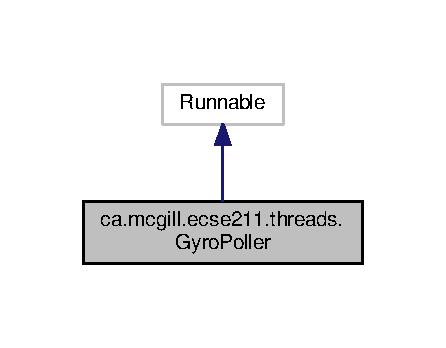
\includegraphics[width=214pt]{classca_1_1mcgill_1_1ecse211_1_1threads_1_1_gyro_poller__inherit__graph}
\end{center}
\end{figure}


Collaboration diagram for ca.\+mcgill.\+ecse211.\+threads.\+Gyro\+Poller\+:
\nopagebreak
\begin{figure}[H]
\begin{center}
\leavevmode
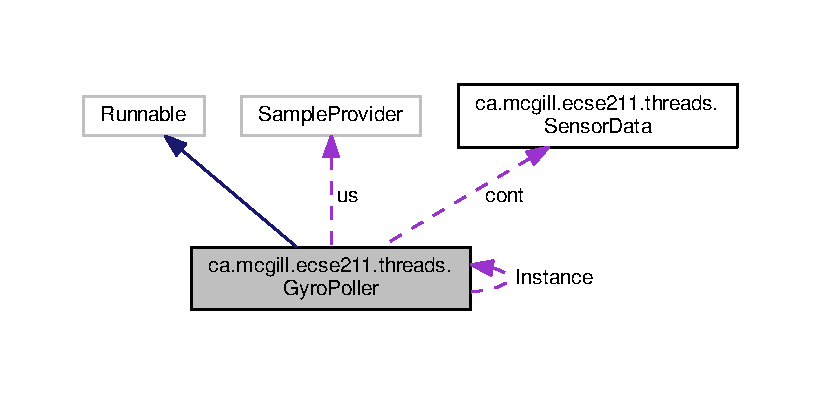
\includegraphics[width=350pt]{classca_1_1mcgill_1_1ecse211_1_1threads_1_1_gyro_poller__coll__graph}
\end{center}
\end{figure}
\subsection*{Public Member Functions}
\begin{DoxyCompactItemize}
\item 
\hyperlink{classca_1_1mcgill_1_1ecse211_1_1threads_1_1_gyro_poller_a1bab49cc19ee3b633ddbec4c408927bf}{Gyro\+Poller} (Sample\+Provider us, float\mbox{[}$\,$\mbox{]} lg\+Data, \hyperlink{classca_1_1mcgill_1_1ecse211_1_1threads_1_1_sensor_data}{Sensor\+Data} cont)  throws Odometer\+Exceptions 
\item 
void \hyperlink{classca_1_1mcgill_1_1ecse211_1_1threads_1_1_gyro_poller_a7a3232e355cece714fa85a3a902d9cfd}{run} ()
\end{DoxyCompactItemize}
\subsection*{Public Attributes}
\begin{DoxyCompactItemize}
\item 
\mbox{\Hypertarget{classca_1_1mcgill_1_1ecse211_1_1threads_1_1_gyro_poller_a181979440aafff52b0ba5aaff9064f80}\label{classca_1_1mcgill_1_1ecse211_1_1threads_1_1_gyro_poller_a181979440aafff52b0ba5aaff9064f80}} 
\hyperlink{classca_1_1mcgill_1_1ecse211_1_1threads_1_1_gyro_poller}{Gyro\+Poller} {\bfseries Instance}
\end{DoxyCompactItemize}
\subsection*{Protected Member Functions}
\begin{DoxyCompactItemize}
\item 
\mbox{\Hypertarget{classca_1_1mcgill_1_1ecse211_1_1threads_1_1_gyro_poller_a27f914ed77f23805210998fc0ee2daa7}\label{classca_1_1mcgill_1_1ecse211_1_1threads_1_1_gyro_poller_a27f914ed77f23805210998fc0ee2daa7}} 
void {\bfseries process\+Data} ()
\end{DoxyCompactItemize}
\subsection*{Protected Attributes}
\begin{DoxyCompactItemize}
\item 
\mbox{\Hypertarget{classca_1_1mcgill_1_1ecse211_1_1threads_1_1_gyro_poller_af478329ec7a335a4f3d2d412d5d10091}\label{classca_1_1mcgill_1_1ecse211_1_1threads_1_1_gyro_poller_af478329ec7a335a4f3d2d412d5d10091}} 
Sample\+Provider {\bfseries us}
\item 
\mbox{\Hypertarget{classca_1_1mcgill_1_1ecse211_1_1threads_1_1_gyro_poller_a90507a3d6038ff7ec7881640b5dd4263}\label{classca_1_1mcgill_1_1ecse211_1_1threads_1_1_gyro_poller_a90507a3d6038ff7ec7881640b5dd4263}} 
\hyperlink{classca_1_1mcgill_1_1ecse211_1_1threads_1_1_sensor_data}{Sensor\+Data} {\bfseries cont}
\item 
\mbox{\Hypertarget{classca_1_1mcgill_1_1ecse211_1_1threads_1_1_gyro_poller_a112e433b3561e89927357051f55f8cf1}\label{classca_1_1mcgill_1_1ecse211_1_1threads_1_1_gyro_poller_a112e433b3561e89927357051f55f8cf1}} 
float \mbox{[}$\,$\mbox{]} {\bfseries lg\+Data}
\end{DoxyCompactItemize}


\subsection{Detailed Description}
This class helps our robot to navigate using a gyroscope $<$Not using, deprecated$>$ \begin{DoxyAuthor}{Author}
Caspar Cedro 

Percy Chen 

Patrick Erath 

Anssam Ghezala 

Susan Matuszewski 

Kamy Moussavi Kafi 
\end{DoxyAuthor}


Definition at line 16 of file Gyro\+Poller.\+java.



\subsection{Constructor \& Destructor Documentation}
\mbox{\Hypertarget{classca_1_1mcgill_1_1ecse211_1_1threads_1_1_gyro_poller_a1bab49cc19ee3b633ddbec4c408927bf}\label{classca_1_1mcgill_1_1ecse211_1_1threads_1_1_gyro_poller_a1bab49cc19ee3b633ddbec4c408927bf}} 
\index{ca\+::mcgill\+::ecse211\+::threads\+::\+Gyro\+Poller@{ca\+::mcgill\+::ecse211\+::threads\+::\+Gyro\+Poller}!Gyro\+Poller@{Gyro\+Poller}}
\index{Gyro\+Poller@{Gyro\+Poller}!ca\+::mcgill\+::ecse211\+::threads\+::\+Gyro\+Poller@{ca\+::mcgill\+::ecse211\+::threads\+::\+Gyro\+Poller}}
\subsubsection{\texorpdfstring{Gyro\+Poller()}{GyroPoller()}}
{\footnotesize\ttfamily ca.\+mcgill.\+ecse211.\+threads.\+Gyro\+Poller.\+Gyro\+Poller (\begin{DoxyParamCaption}\item[{Sample\+Provider}]{us,  }\item[{float \mbox{[}$\,$\mbox{]}}]{lg\+Data,  }\item[{\hyperlink{classca_1_1mcgill_1_1ecse211_1_1threads_1_1_sensor_data}{Sensor\+Data}}]{cont }\end{DoxyParamCaption}) throws \hyperlink{classca_1_1mcgill_1_1ecse211_1_1odometer_1_1_odometer_exceptions}{Odometer\+Exceptions}}

This constructor creates an instance of the \hyperlink{classca_1_1mcgill_1_1ecse211_1_1threads_1_1_gyro_poller}{Gyro\+Poller} class to aid navigation


\begin{DoxyParams}{Parameters}
{\em us} & A Sample\+Provider class instance that helps us to store an array of ultrasonic sensor data. \\
\hline
{\em lg\+Data} & An array used to store data. \\
\hline
{\em cont} & A \hyperlink{classca_1_1mcgill_1_1ecse211_1_1threads_1_1_sensor_data}{Sensor\+Data} object instance used to manage sensor data. \\
\hline
\end{DoxyParams}

\begin{DoxyExceptions}{Exceptions}
{\em Odometer\+Exceptions} & \\
\hline
\end{DoxyExceptions}


Definition at line 31 of file Gyro\+Poller.\+java.



\subsection{Member Function Documentation}
\mbox{\Hypertarget{classca_1_1mcgill_1_1ecse211_1_1threads_1_1_gyro_poller_a7a3232e355cece714fa85a3a902d9cfd}\label{classca_1_1mcgill_1_1ecse211_1_1threads_1_1_gyro_poller_a7a3232e355cece714fa85a3a902d9cfd}} 
\index{ca\+::mcgill\+::ecse211\+::threads\+::\+Gyro\+Poller@{ca\+::mcgill\+::ecse211\+::threads\+::\+Gyro\+Poller}!run@{run}}
\index{run@{run}!ca\+::mcgill\+::ecse211\+::threads\+::\+Gyro\+Poller@{ca\+::mcgill\+::ecse211\+::threads\+::\+Gyro\+Poller}}
\subsubsection{\texorpdfstring{run()}{run()}}
{\footnotesize\ttfamily void ca.\+mcgill.\+ecse211.\+threads.\+Gyro\+Poller.\+run (\begin{DoxyParamCaption}{ }\end{DoxyParamCaption})}

This method is called by a \hyperlink{classca_1_1mcgill_1_1ecse211_1_1threads_1_1_ultrasonic_poller}{Ultrasonic\+Poller} (Thread) instance when it is asked to start executing

Sensors now return floats using a uniform protocol. Need to convert US result to an integer \mbox{[}0,255\mbox{]} (non-\/\+Javadoc)

\begin{DoxySeeAlso}{See also}
java.\+lang.\+Thread\+::run() 
\end{DoxySeeAlso}


Definition at line 46 of file Gyro\+Poller.\+java.

Here is the call graph for this function\+:
\nopagebreak
\begin{figure}[H]
\begin{center}
\leavevmode
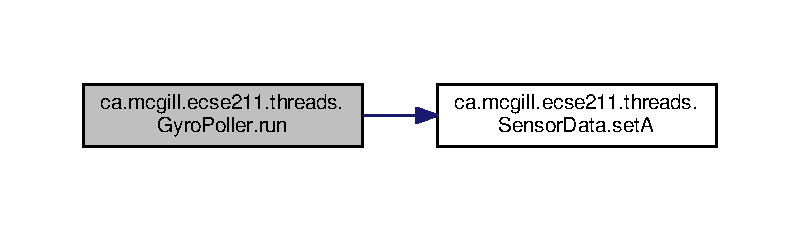
\includegraphics[width=350pt]{classca_1_1mcgill_1_1ecse211_1_1threads_1_1_gyro_poller_a7a3232e355cece714fa85a3a902d9cfd_cgraph}
\end{center}
\end{figure}


The documentation for this class was generated from the following file\+:\begin{DoxyCompactItemize}
\item 
/home/ccc/\+Final\+Project/src/ca/mcgill/ecse211/threads/Gyro\+Poller.\+java\end{DoxyCompactItemize}

\hypertarget{classca_1_1mcgill_1_1ecse211_1_1localization_1_1_light_localizer}{}\section{ca.\+mcgill.\+ecse211.\+localization.\+Light\+Localizer Class Reference}
\label{classca_1_1mcgill_1_1ecse211_1_1localization_1_1_light_localizer}\index{ca.\+mcgill.\+ecse211.\+localization.\+Light\+Localizer@{ca.\+mcgill.\+ecse211.\+localization.\+Light\+Localizer}}
\subsection*{Public Member Functions}
\begin{DoxyCompactItemize}
\item 
\hyperlink{classca_1_1mcgill_1_1ecse211_1_1localization_1_1_light_localizer_aa37a75b7c32c02fe261845021f0734b7}{Light\+Localizer} (\hyperlink{classca_1_1mcgill_1_1ecse211_1_1project_1_1_navigation}{Navigation} nav, E\+V3\+Large\+Regulated\+Motor left\+Motor, E\+V3\+Large\+Regulated\+Motor right\+Motor)  throws Odometer\+Exceptions 
\item 
void \hyperlink{classca_1_1mcgill_1_1ecse211_1_1localization_1_1_light_localizer_a9fc3d6cdd897e9db86fc9d71dc914863}{localize} (int\mbox{[}$\,$\mbox{]} sC)
\end{DoxyCompactItemize}


\subsection{Detailed Description}
This class helps our robot to localize itself using the light sensor

\begin{DoxyAuthor}{Author}
Caspar Cedro 

Percy Chen 

Patrick Erath 

Anssam Ghezala 

Susan Matuszewski 

Kamy Moussavi Kafi 
\end{DoxyAuthor}


Definition at line 21 of file Light\+Localizer.\+java.



\subsection{Constructor \& Destructor Documentation}
\mbox{\Hypertarget{classca_1_1mcgill_1_1ecse211_1_1localization_1_1_light_localizer_aa37a75b7c32c02fe261845021f0734b7}\label{classca_1_1mcgill_1_1ecse211_1_1localization_1_1_light_localizer_aa37a75b7c32c02fe261845021f0734b7}} 
\index{ca\+::mcgill\+::ecse211\+::localization\+::\+Light\+Localizer@{ca\+::mcgill\+::ecse211\+::localization\+::\+Light\+Localizer}!Light\+Localizer@{Light\+Localizer}}
\index{Light\+Localizer@{Light\+Localizer}!ca\+::mcgill\+::ecse211\+::localization\+::\+Light\+Localizer@{ca\+::mcgill\+::ecse211\+::localization\+::\+Light\+Localizer}}
\subsubsection{\texorpdfstring{Light\+Localizer()}{LightLocalizer()}}
{\footnotesize\ttfamily ca.\+mcgill.\+ecse211.\+localization.\+Light\+Localizer.\+Light\+Localizer (\begin{DoxyParamCaption}\item[{\hyperlink{classca_1_1mcgill_1_1ecse211_1_1project_1_1_navigation}{Navigation}}]{nav,  }\item[{E\+V3\+Large\+Regulated\+Motor}]{left\+Motor,  }\item[{E\+V3\+Large\+Regulated\+Motor}]{right\+Motor }\end{DoxyParamCaption}) throws \hyperlink{classca_1_1mcgill_1_1ecse211_1_1odometer_1_1_odometer_exceptions}{Odometer\+Exceptions}}

This is the class constructor


\begin{DoxyParams}{Parameters}
{\em left\+Motor} & \\
\hline
{\em right\+Motor} & \\
\hline
\end{DoxyParams}

\begin{DoxyExceptions}{Exceptions}
{\em Odometer\+Exceptions} & \\
\hline
\end{DoxyExceptions}


Definition at line 38 of file Light\+Localizer.\+java.


\begin{DoxyCode}
39                                                                    \{
40     this.odometer = Odometer.\hyperlink{classca_1_1mcgill_1_1ecse211_1_1odometer_1_1_odometer_a99171f11e34dea918fa9dd069d721439}{getOdometer}();
41     this.data = SensorData.\hyperlink{classca_1_1mcgill_1_1ecse211_1_1threads_1_1_sensor_data_a8260aba53b4474ca1275e4ce26157977}{getSensorData}();
42     this.navigation = nav;
43     this.leftMotor = leftMotor;
44     this.rightMotor = rightMotor;
45   \}
\end{DoxyCode}
Here is the call graph for this function\+:\nopagebreak
\begin{figure}[H]
\begin{center}
\leavevmode
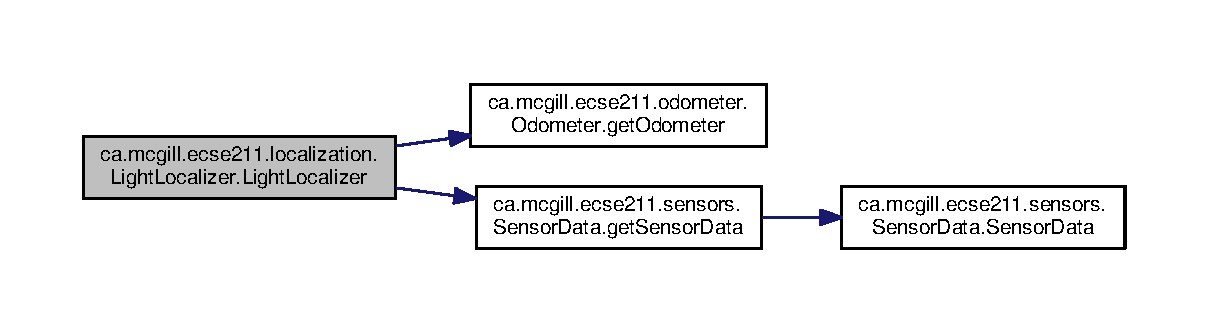
\includegraphics[width=350pt]{classca_1_1mcgill_1_1ecse211_1_1localization_1_1_light_localizer_aa37a75b7c32c02fe261845021f0734b7_cgraph}
\end{center}
\end{figure}


\subsection{Member Function Documentation}
\mbox{\Hypertarget{classca_1_1mcgill_1_1ecse211_1_1localization_1_1_light_localizer_a9fc3d6cdd897e9db86fc9d71dc914863}\label{classca_1_1mcgill_1_1ecse211_1_1localization_1_1_light_localizer_a9fc3d6cdd897e9db86fc9d71dc914863}} 
\index{ca\+::mcgill\+::ecse211\+::localization\+::\+Light\+Localizer@{ca\+::mcgill\+::ecse211\+::localization\+::\+Light\+Localizer}!localize@{localize}}
\index{localize@{localize}!ca\+::mcgill\+::ecse211\+::localization\+::\+Light\+Localizer@{ca\+::mcgill\+::ecse211\+::localization\+::\+Light\+Localizer}}
\subsubsection{\texorpdfstring{localize()}{localize()}}
{\footnotesize\ttfamily void ca.\+mcgill.\+ecse211.\+localization.\+Light\+Localizer.\+localize (\begin{DoxyParamCaption}\item[{int \mbox{[}$\,$\mbox{]}}]{sC }\end{DoxyParamCaption})}

({\itshape Improve}) Once the robot know what angle it is facing, this method looks for the x,y axis origins knowing it is in the first tile facing north. 
\begin{DoxyParams}{Parameters}
{\em sC} & the coordinate to set to after localization \\
\hline
\end{DoxyParams}


Definition at line 53 of file Light\+Localizer.\+java.


\begin{DoxyCode}
53                                  \{
54     leftMotor.setSpeed(FORWARD\_SPEED);
55     rightMotor.setSpeed(FORWARD\_SPEED);
56 
57     \textcolor{comment}{// 1. GO forward find the y=0 line}
58     leftMotor.forward();
59     rightMotor.forward();
60     \textcolor{keywordflow}{while} (data.\hyperlink{classca_1_1mcgill_1_1ecse211_1_1threads_1_1_sensor_data_a39eec50582f0e4bcff8a4669c48e1609}{getL}()[0] > blackLineColor);
61     Sound.beep();
62     odometer.\hyperlink{classca_1_1mcgill_1_1ecse211_1_1odometer_1_1_odometer_data_a82986438cd462e66520bc62bb4bd2b75}{setY}(0);
63     \textcolor{comment}{// 2. Turn and go forward find the x=0 line}
64     navigation.\hyperlink{classca_1_1mcgill_1_1ecse211_1_1project_1_1_navigation_a3bbe0645f2b3b3d0986b4a707fb5a00c}{turnTo}(90);
65     leftMotor.setSpeed(FORWARD\_SPEED / 2);
66     rightMotor.setSpeed(FORWARD\_SPEED / 2);
67     leftMotor.forward();
68     rightMotor.forward();
69     \textcolor{keywordflow}{while} (data.\hyperlink{classca_1_1mcgill_1_1ecse211_1_1threads_1_1_sensor_data_a39eec50582f0e4bcff8a4669c48e1609}{getL}()[0] > blackLineColor);
70     Sound.beep();
71     odometer.\hyperlink{classca_1_1mcgill_1_1ecse211_1_1odometer_1_1_odometer_data_a2911d7215e47f3064defe016b46bfeef}{setX}(0);
72     leftMotor.setSpeed(FORWARD\_SPEED / 2);
73     rightMotor.setSpeed(FORWARD\_SPEED / 2);
74     \textcolor{comment}{// 3. Go backwards by sensor-wheel center distance in x-direction}
75     leftMotor.rotate(Navigation.convertDistance(Game.WHEEL\_RAD, -SENSOR\_DIS), \textcolor{keyword}{true});
76     rightMotor.rotate(Navigation.convertDistance(Game.WHEEL\_RAD, -SENSOR\_DIS), \textcolor{keyword}{false});
77     \textcolor{comment}{// 4. Go backwards by sensor-wheel center distance in y-direction}
78     navigation.\hyperlink{classca_1_1mcgill_1_1ecse211_1_1project_1_1_navigation_a3bbe0645f2b3b3d0986b4a707fb5a00c}{turnTo}(0);
79     leftMotor.setSpeed(FORWARD\_SPEED / 2);
80     rightMotor.setSpeed(FORWARD\_SPEED / 2);
81     \textcolor{keywordtype}{double} sensorDistanceOffset = 2.5;
82     leftMotor.rotate(
83         Navigation.convertDistance(Game.WHEEL\_RAD, -SENSOR\_DIS - sensorDistanceOffset),
84         \textcolor{keyword}{true});
85     rightMotor.rotate(
86         Navigation.convertDistance(Game.WHEEL\_RAD, -SENSOR\_DIS - sensorDistanceOffset),
87         \textcolor{keyword}{false});
88     odometer.\hyperlink{classca_1_1mcgill_1_1ecse211_1_1odometer_1_1_odometer_data_a419b8f07c2c5374411c8e62298e9a402}{setTheta}(0);
89     odometer.\hyperlink{classca_1_1mcgill_1_1ecse211_1_1odometer_1_1_odometer_data_a2911d7215e47f3064defe016b46bfeef}{setX}(sC[0]);
90     odometer.\hyperlink{classca_1_1mcgill_1_1ecse211_1_1odometer_1_1_odometer_data_a82986438cd462e66520bc62bb4bd2b75}{setY}(sC[1]);
91 
92   \}
\end{DoxyCode}
Here is the call graph for this function\+:\nopagebreak
\begin{figure}[H]
\begin{center}
\leavevmode
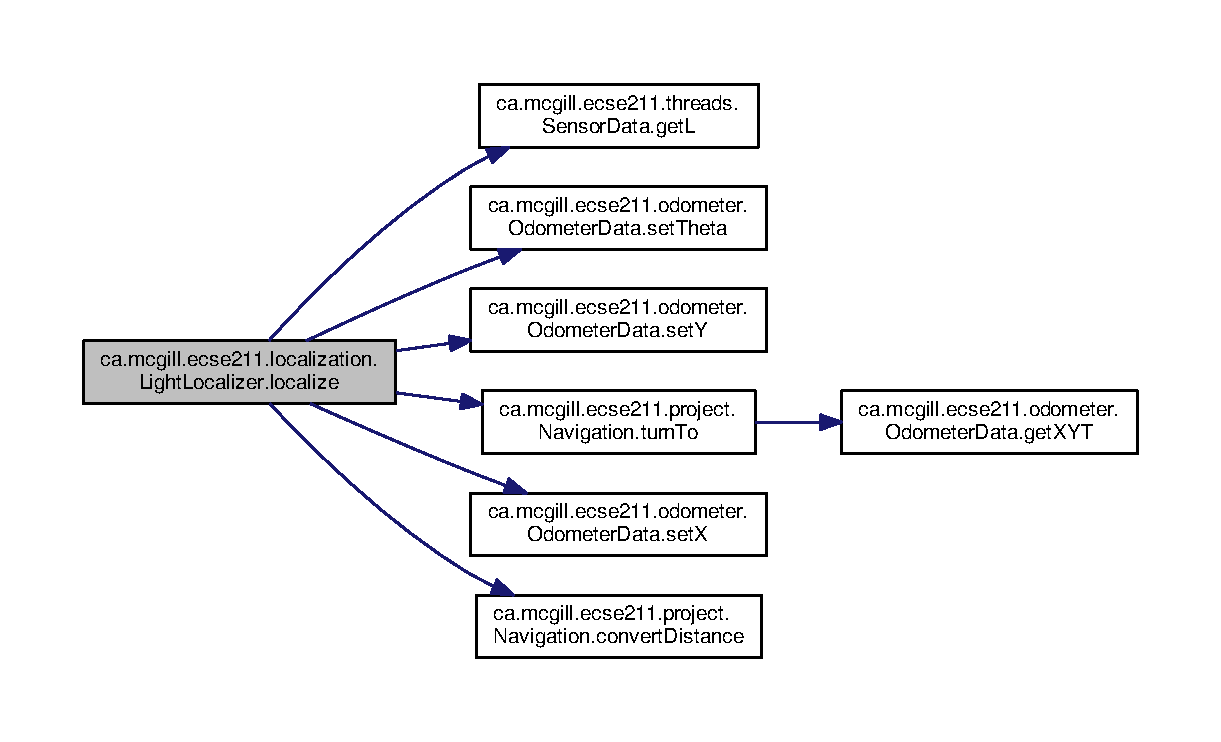
\includegraphics[width=350pt]{classca_1_1mcgill_1_1ecse211_1_1localization_1_1_light_localizer_a9fc3d6cdd897e9db86fc9d71dc914863_cgraph}
\end{center}
\end{figure}
Here is the caller graph for this function\+:\nopagebreak
\begin{figure}[H]
\begin{center}
\leavevmode
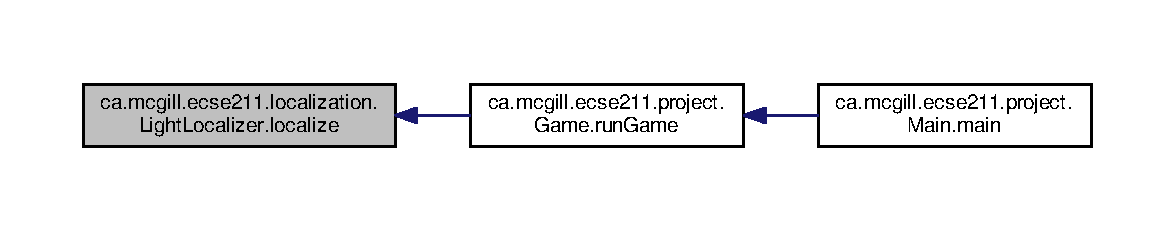
\includegraphics[width=350pt]{classca_1_1mcgill_1_1ecse211_1_1localization_1_1_light_localizer_a9fc3d6cdd897e9db86fc9d71dc914863_icgraph}
\end{center}
\end{figure}


The documentation for this class was generated from the following file\+:\begin{DoxyCompactItemize}
\item 
/home/ccc/\+Final\+Project/src/ca/mcgill/ecse211/localization/\hyperlink{_light_localizer_8java}{Light\+Localizer.\+java}\end{DoxyCompactItemize}

\hypertarget{classca_1_1mcgill_1_1ecse211_1_1threads_1_1_light_poller}{}\section{ca.\+mcgill.\+ecse211.\+threads.\+Light\+Poller Class Reference}
\label{classca_1_1mcgill_1_1ecse211_1_1threads_1_1_light_poller}\index{ca.\+mcgill.\+ecse211.\+threads.\+Light\+Poller@{ca.\+mcgill.\+ecse211.\+threads.\+Light\+Poller}}


Inheritance diagram for ca.\+mcgill.\+ecse211.\+threads.\+Light\+Poller\+:\nopagebreak
\begin{figure}[H]
\begin{center}
\leavevmode
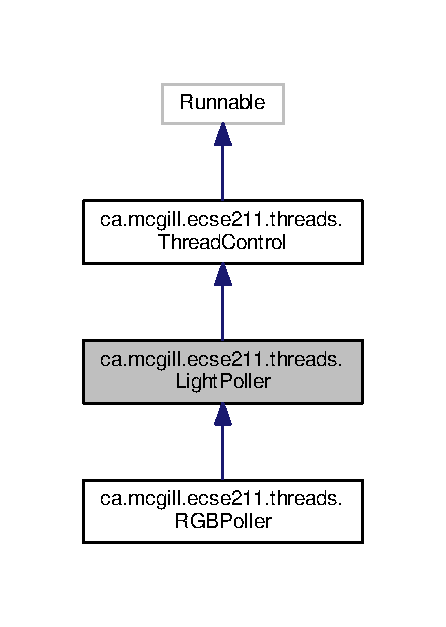
\includegraphics[width=214pt]{classca_1_1mcgill_1_1ecse211_1_1threads_1_1_light_poller__inherit__graph}
\end{center}
\end{figure}


Collaboration diagram for ca.\+mcgill.\+ecse211.\+threads.\+Light\+Poller\+:\nopagebreak
\begin{figure}[H]
\begin{center}
\leavevmode
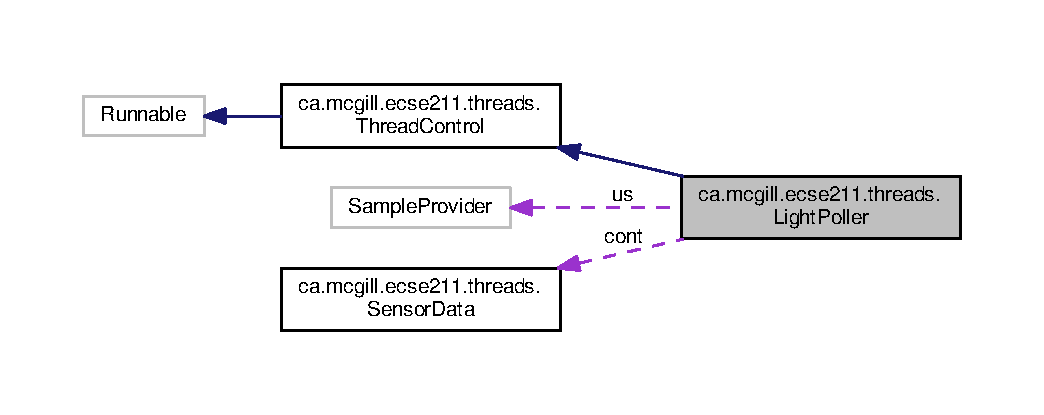
\includegraphics[width=350pt]{classca_1_1mcgill_1_1ecse211_1_1threads_1_1_light_poller__coll__graph}
\end{center}
\end{figure}
\subsection*{Public Member Functions}
\begin{DoxyCompactItemize}
\item 
\hyperlink{classca_1_1mcgill_1_1ecse211_1_1threads_1_1_light_poller_adc07f842a1cc089195c5e47c2a0e5ee6}{Light\+Poller} (Sample\+Provider\mbox{[}$\,$\mbox{]} \hyperlink{classca_1_1mcgill_1_1ecse211_1_1threads_1_1_light_poller_ab6a9cb770bbf71f586697633db1475ff}{us}, float\mbox{[}$\,$\mbox{]}\mbox{[}$\,$\mbox{]} \hyperlink{classca_1_1mcgill_1_1ecse211_1_1threads_1_1_light_poller_a6cf53aecc3efc481f71d36341d2276c6}{lg\+Data}, \hyperlink{classca_1_1mcgill_1_1ecse211_1_1threads_1_1_sensor_data}{Sensor\+Data} \hyperlink{classca_1_1mcgill_1_1ecse211_1_1threads_1_1_light_poller_ab6a9050ced4f6940add4735c8872194a}{cont})  throws Odometer\+Exceptions 
\end{DoxyCompactItemize}
\subsection*{Protected Member Functions}
\begin{DoxyCompactItemize}
\item 
void \hyperlink{classca_1_1mcgill_1_1ecse211_1_1threads_1_1_light_poller_aab90a460a4d0c926fb8f3930492a8fb1}{run\+Method} ()
\end{DoxyCompactItemize}
\subsection*{Protected Attributes}
\begin{DoxyCompactItemize}
\item 
Sample\+Provider \hyperlink{classca_1_1mcgill_1_1ecse211_1_1threads_1_1_light_poller_ab6a9cb770bbf71f586697633db1475ff}{us} \mbox{[}$\,$\mbox{]}
\item 
\hyperlink{classca_1_1mcgill_1_1ecse211_1_1threads_1_1_sensor_data}{Sensor\+Data} \hyperlink{classca_1_1mcgill_1_1ecse211_1_1threads_1_1_light_poller_ab6a9050ced4f6940add4735c8872194a}{cont}
\item 
float \mbox{[}$\,$\mbox{]}\mbox{[}$\,$\mbox{]} \hyperlink{classca_1_1mcgill_1_1ecse211_1_1threads_1_1_light_poller_a6cf53aecc3efc481f71d36341d2276c6}{lg\+Data}
\item 
float \hyperlink{classca_1_1mcgill_1_1ecse211_1_1threads_1_1_light_poller_a79908bf56395ae82ab5ac57b5b40f206}{last\+Value} \mbox{[}$\,$\mbox{]}
\end{DoxyCompactItemize}
\subsection*{Additional Inherited Members}


\subsection{Detailed Description}
This class implements the Light Sensor Poller for our robot it runs pulls the sensor data every 50 miliseconds

\begin{DoxyAuthor}{Author}
Caspar Cedro 

Percy Chen 

Patrick Erath 

Anssam Ghezala 

Susan Matuszewski 

Kamy Moussavi Kafi 
\end{DoxyAuthor}


Definition at line 17 of file Light\+Poller.\+java.



\subsection{Constructor \& Destructor Documentation}
\mbox{\Hypertarget{classca_1_1mcgill_1_1ecse211_1_1threads_1_1_light_poller_adc07f842a1cc089195c5e47c2a0e5ee6}\label{classca_1_1mcgill_1_1ecse211_1_1threads_1_1_light_poller_adc07f842a1cc089195c5e47c2a0e5ee6}} 
\index{ca\+::mcgill\+::ecse211\+::threads\+::\+Light\+Poller@{ca\+::mcgill\+::ecse211\+::threads\+::\+Light\+Poller}!Light\+Poller@{Light\+Poller}}
\index{Light\+Poller@{Light\+Poller}!ca\+::mcgill\+::ecse211\+::threads\+::\+Light\+Poller@{ca\+::mcgill\+::ecse211\+::threads\+::\+Light\+Poller}}
\subsubsection{\texorpdfstring{Light\+Poller()}{LightPoller()}}
{\footnotesize\ttfamily ca.\+mcgill.\+ecse211.\+threads.\+Light\+Poller.\+Light\+Poller (\begin{DoxyParamCaption}\item[{Sample\+Provider \mbox{[}$\,$\mbox{]}}]{us,  }\item[{float}]{lg\+Data\mbox{[}$\,$\mbox{]}\mbox{[}$\,$\mbox{]},  }\item[{\hyperlink{classca_1_1mcgill_1_1ecse211_1_1threads_1_1_sensor_data}{Sensor\+Data}}]{cont }\end{DoxyParamCaption}) throws \hyperlink{classca_1_1mcgill_1_1ecse211_1_1odometer_1_1_odometer_exceptions}{Odometer\+Exceptions}}

This constructor creates an instance of the \hyperlink{classca_1_1mcgill_1_1ecse211_1_1threads_1_1_light_poller}{Light\+Poller} class to provide distance data from an light sensor to our robot.


\begin{DoxyParams}{Parameters}
{\em us} & a Sample\+Provider class instance that helps us to store an array of ultrasonic sensor data. \\
\hline
{\em lg\+Data} & an array of distance data to be used by our Wall Follower\textquotesingle{}s Ultrasonic\+Controllers. \\
\hline
{\em cont} & a Bang\+Bang\+Controller or P\+Controller instance that has accumulated distance data stored in us\+Data passed to it. \\
\hline
\end{DoxyParams}

\begin{DoxyExceptions}{Exceptions}
{\em Odometer\+Exceptions} & \\
\hline
\end{DoxyExceptions}


Definition at line 36 of file Light\+Poller.\+java.


\begin{DoxyCode}
37                                 \{
38     this.\hyperlink{classca_1_1mcgill_1_1ecse211_1_1threads_1_1_light_poller_ab6a9cb770bbf71f586697633db1475ff}{us} = \hyperlink{classca_1_1mcgill_1_1ecse211_1_1threads_1_1_light_poller_ab6a9cb770bbf71f586697633db1475ff}{us};
39     this.\hyperlink{classca_1_1mcgill_1_1ecse211_1_1threads_1_1_light_poller_ab6a9050ced4f6940add4735c8872194a}{cont} = \hyperlink{classca_1_1mcgill_1_1ecse211_1_1threads_1_1_light_poller_ab6a9050ced4f6940add4735c8872194a}{cont};
40     this.\hyperlink{classca_1_1mcgill_1_1ecse211_1_1threads_1_1_light_poller_a6cf53aecc3efc481f71d36341d2276c6}{lgData} = \hyperlink{classca_1_1mcgill_1_1ecse211_1_1threads_1_1_light_poller_a6cf53aecc3efc481f71d36341d2276c6}{lgData};
41     \hyperlink{classca_1_1mcgill_1_1ecse211_1_1threads_1_1_thread_control_a92f4933511db42476e39956246bcf2fe}{isStarted} = \textcolor{keyword}{true};
42     \hyperlink{classca_1_1mcgill_1_1ecse211_1_1threads_1_1_light_poller_a79908bf56395ae82ab5ac57b5b40f206}{lastValue} = \textcolor{keyword}{new} \textcolor{keywordtype}{float}[2];
43     sensorNumber++;
44     \hyperlink{classca_1_1mcgill_1_1ecse211_1_1threads_1_1_thread_control_a395cfe1d73b3ef14da0830ed0a499f82}{WAIT\_TIME} = 50;
45   \}
\end{DoxyCode}
Here is the call graph for this function\+:\nopagebreak
\begin{figure}[H]
\begin{center}
\leavevmode
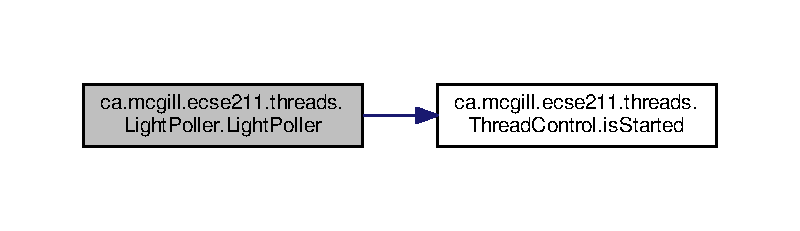
\includegraphics[width=350pt]{classca_1_1mcgill_1_1ecse211_1_1threads_1_1_light_poller_adc07f842a1cc089195c5e47c2a0e5ee6_cgraph}
\end{center}
\end{figure}


\subsection{Member Function Documentation}
\mbox{\Hypertarget{classca_1_1mcgill_1_1ecse211_1_1threads_1_1_light_poller_aab90a460a4d0c926fb8f3930492a8fb1}\label{classca_1_1mcgill_1_1ecse211_1_1threads_1_1_light_poller_aab90a460a4d0c926fb8f3930492a8fb1}} 
\index{ca\+::mcgill\+::ecse211\+::threads\+::\+Light\+Poller@{ca\+::mcgill\+::ecse211\+::threads\+::\+Light\+Poller}!run\+Method@{run\+Method}}
\index{run\+Method@{run\+Method}!ca\+::mcgill\+::ecse211\+::threads\+::\+Light\+Poller@{ca\+::mcgill\+::ecse211\+::threads\+::\+Light\+Poller}}
\subsubsection{\texorpdfstring{run\+Method()}{runMethod()}}
{\footnotesize\ttfamily void ca.\+mcgill.\+ecse211.\+threads.\+Light\+Poller.\+run\+Method (\begin{DoxyParamCaption}{ }\end{DoxyParamCaption})\hspace{0.3cm}{\ttfamily [protected]}}

the run method to be performed in run method, collect light data 

Definition at line 50 of file Light\+Poller.\+java.


\begin{DoxyCode}
50                              \{
51     \textcolor{keywordtype}{double} l[] = \textcolor{keyword}{new} \textcolor{keywordtype}{double}[2];
52     \textcolor{keywordflow}{for} (\textcolor{keywordtype}{int} i = 0; i < \hyperlink{classca_1_1mcgill_1_1ecse211_1_1threads_1_1_light_poller_ab6a9cb770bbf71f586697633db1475ff}{us}.length; i++) \{
53       \hyperlink{classca_1_1mcgill_1_1ecse211_1_1threads_1_1_light_poller_ab6a9cb770bbf71f586697633db1475ff}{us}[i].fetchSample(\hyperlink{classca_1_1mcgill_1_1ecse211_1_1threads_1_1_light_poller_a6cf53aecc3efc481f71d36341d2276c6}{lgData}[i], 0); \textcolor{comment}{// acquire data}
54 
55       \textcolor{keywordtype}{int} distance = (int) (\hyperlink{classca_1_1mcgill_1_1ecse211_1_1threads_1_1_light_poller_a6cf53aecc3efc481f71d36341d2276c6}{lgData}[i][0] * 100); \textcolor{comment}{// extract from buffer, multiply by 100 for}
56                                                  \textcolor{comment}{// convenience}
57       \textcolor{comment}{// and allow it to be cast to int}
58       l[i] = distance - \hyperlink{classca_1_1mcgill_1_1ecse211_1_1threads_1_1_light_poller_a79908bf56395ae82ab5ac57b5b40f206}{lastValue}[i]; \textcolor{comment}{// now take action depending on value}
59       lastValue[i] = distance;
60     \}
61     \hyperlink{classca_1_1mcgill_1_1ecse211_1_1threads_1_1_light_poller_ab6a9050ced4f6940add4735c8872194a}{cont}.\hyperlink{classca_1_1mcgill_1_1ecse211_1_1threads_1_1_sensor_data_af905a6f2825716ae1a39bf7f6be09477}{setL}(l);
62   \}
\end{DoxyCode}
Here is the call graph for this function\+:\nopagebreak
\begin{figure}[H]
\begin{center}
\leavevmode
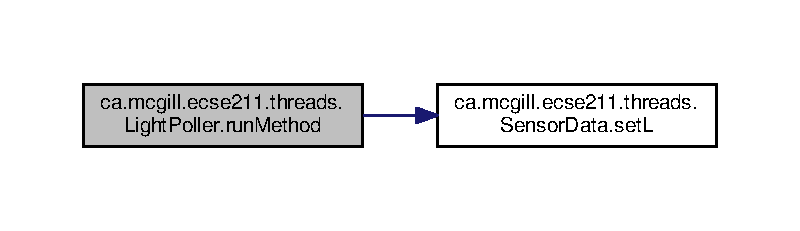
\includegraphics[width=350pt]{classca_1_1mcgill_1_1ecse211_1_1threads_1_1_light_poller_aab90a460a4d0c926fb8f3930492a8fb1_cgraph}
\end{center}
\end{figure}


\subsection{Member Data Documentation}
\mbox{\Hypertarget{classca_1_1mcgill_1_1ecse211_1_1threads_1_1_light_poller_ab6a9050ced4f6940add4735c8872194a}\label{classca_1_1mcgill_1_1ecse211_1_1threads_1_1_light_poller_ab6a9050ced4f6940add4735c8872194a}} 
\index{ca\+::mcgill\+::ecse211\+::threads\+::\+Light\+Poller@{ca\+::mcgill\+::ecse211\+::threads\+::\+Light\+Poller}!cont@{cont}}
\index{cont@{cont}!ca\+::mcgill\+::ecse211\+::threads\+::\+Light\+Poller@{ca\+::mcgill\+::ecse211\+::threads\+::\+Light\+Poller}}
\subsubsection{\texorpdfstring{cont}{cont}}
{\footnotesize\ttfamily \hyperlink{classca_1_1mcgill_1_1ecse211_1_1threads_1_1_sensor_data}{Sensor\+Data} ca.\+mcgill.\+ecse211.\+threads.\+Light\+Poller.\+cont\hspace{0.3cm}{\ttfamily [protected]}}



Definition at line 19 of file Light\+Poller.\+java.

\mbox{\Hypertarget{classca_1_1mcgill_1_1ecse211_1_1threads_1_1_light_poller_a79908bf56395ae82ab5ac57b5b40f206}\label{classca_1_1mcgill_1_1ecse211_1_1threads_1_1_light_poller_a79908bf56395ae82ab5ac57b5b40f206}} 
\index{ca\+::mcgill\+::ecse211\+::threads\+::\+Light\+Poller@{ca\+::mcgill\+::ecse211\+::threads\+::\+Light\+Poller}!last\+Value@{last\+Value}}
\index{last\+Value@{last\+Value}!ca\+::mcgill\+::ecse211\+::threads\+::\+Light\+Poller@{ca\+::mcgill\+::ecse211\+::threads\+::\+Light\+Poller}}
\subsubsection{\texorpdfstring{last\+Value}{lastValue}}
{\footnotesize\ttfamily float ca.\+mcgill.\+ecse211.\+threads.\+Light\+Poller.\+last\+Value\mbox{[}$\,$\mbox{]}\hspace{0.3cm}{\ttfamily [protected]}}



Definition at line 21 of file Light\+Poller.\+java.

\mbox{\Hypertarget{classca_1_1mcgill_1_1ecse211_1_1threads_1_1_light_poller_a6cf53aecc3efc481f71d36341d2276c6}\label{classca_1_1mcgill_1_1ecse211_1_1threads_1_1_light_poller_a6cf53aecc3efc481f71d36341d2276c6}} 
\index{ca\+::mcgill\+::ecse211\+::threads\+::\+Light\+Poller@{ca\+::mcgill\+::ecse211\+::threads\+::\+Light\+Poller}!lg\+Data@{lg\+Data}}
\index{lg\+Data@{lg\+Data}!ca\+::mcgill\+::ecse211\+::threads\+::\+Light\+Poller@{ca\+::mcgill\+::ecse211\+::threads\+::\+Light\+Poller}}
\subsubsection{\texorpdfstring{lg\+Data}{lgData}}
{\footnotesize\ttfamily float \mbox{[}$\,$\mbox{]}\mbox{[}$\,$\mbox{]} ca.\+mcgill.\+ecse211.\+threads.\+Light\+Poller.\+lg\+Data\hspace{0.3cm}{\ttfamily [protected]}}



Definition at line 20 of file Light\+Poller.\+java.

\mbox{\Hypertarget{classca_1_1mcgill_1_1ecse211_1_1threads_1_1_light_poller_ab6a9cb770bbf71f586697633db1475ff}\label{classca_1_1mcgill_1_1ecse211_1_1threads_1_1_light_poller_ab6a9cb770bbf71f586697633db1475ff}} 
\index{ca\+::mcgill\+::ecse211\+::threads\+::\+Light\+Poller@{ca\+::mcgill\+::ecse211\+::threads\+::\+Light\+Poller}!us@{us}}
\index{us@{us}!ca\+::mcgill\+::ecse211\+::threads\+::\+Light\+Poller@{ca\+::mcgill\+::ecse211\+::threads\+::\+Light\+Poller}}
\subsubsection{\texorpdfstring{us}{us}}
{\footnotesize\ttfamily Sample\+Provider ca.\+mcgill.\+ecse211.\+threads.\+Light\+Poller.\+us\mbox{[}$\,$\mbox{]}\hspace{0.3cm}{\ttfamily [protected]}}



Definition at line 18 of file Light\+Poller.\+java.



The documentation for this class was generated from the following file\+:\begin{DoxyCompactItemize}
\item 
/home/ccc/\+Final\+Project/src/ca/mcgill/ecse211/threads/\hyperlink{_light_poller_8java}{Light\+Poller.\+java}\end{DoxyCompactItemize}

\hypertarget{classca_1_1mcgill_1_1ecse211_1_1project_1_1_main}{}\section{ca.\+mcgill.\+ecse211.\+project.\+Main Class Reference}
\label{classca_1_1mcgill_1_1ecse211_1_1project_1_1_main}\index{ca.\+mcgill.\+ecse211.\+project.\+Main@{ca.\+mcgill.\+ecse211.\+project.\+Main}}


Collaboration diagram for ca.\+mcgill.\+ecse211.\+project.\+Main\+:\nopagebreak
\begin{figure}[H]
\begin{center}
\leavevmode
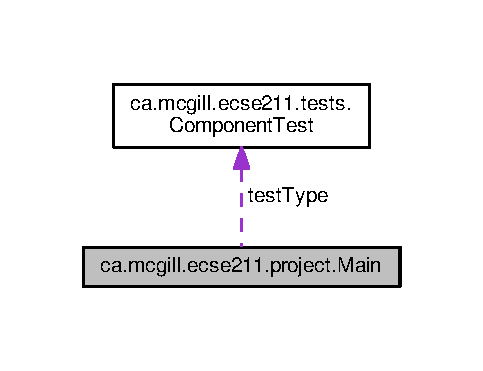
\includegraphics[width=232pt]{classca_1_1mcgill_1_1ecse211_1_1project_1_1_main__coll__graph}
\end{center}
\end{figure}
\subsection*{Static Public Member Functions}
\begin{DoxyCompactItemize}
\item 
static void \hyperlink{classca_1_1mcgill_1_1ecse211_1_1project_1_1_main_af681b5dc675c13ed284071cc135f5fd3}{main} (String\mbox{[}$\,$\mbox{]} args)
\end{DoxyCompactItemize}
\subsection*{Static Public Attributes}
\begin{DoxyCompactItemize}
\item 
static boolean \hyperlink{classca_1_1mcgill_1_1ecse211_1_1project_1_1_main_af6f7b8fffddcf855f74fe128d2e23ea1}{test} = true
\item 
static Component\+Test.\+Type \hyperlink{classca_1_1mcgill_1_1ecse211_1_1project_1_1_main_a8dac740460370f76ac0db5dc20824b1f}{test\+Type} = \hyperlink{enumca_1_1mcgill_1_1ecse211_1_1tests_1_1_component_test_1_1_type_ab118eac94e0b37e6871a4c9a788c675e}{Component\+Test.\+Type.\+Ring\+Detection}
\end{DoxyCompactItemize}


\subsection{Detailed Description}
This class implements the main starting point for our final project

\begin{DoxyAuthor}{Author}
Caspar Cedro 

Percy Chen 

Patrick Erath 

Anssam Ghezala 

Susan Matuszewski 

Kamy Moussavi Kafi 
\end{DoxyAuthor}


Definition at line 17 of file Main.\+java.



\subsection{Member Function Documentation}
\mbox{\Hypertarget{classca_1_1mcgill_1_1ecse211_1_1project_1_1_main_af681b5dc675c13ed284071cc135f5fd3}\label{classca_1_1mcgill_1_1ecse211_1_1project_1_1_main_af681b5dc675c13ed284071cc135f5fd3}} 
\index{ca\+::mcgill\+::ecse211\+::project\+::\+Main@{ca\+::mcgill\+::ecse211\+::project\+::\+Main}!main@{main}}
\index{main@{main}!ca\+::mcgill\+::ecse211\+::project\+::\+Main@{ca\+::mcgill\+::ecse211\+::project\+::\+Main}}
\subsubsection{\texorpdfstring{main()}{main()}}
{\footnotesize\ttfamily static void ca.\+mcgill.\+ecse211.\+project.\+Main.\+main (\begin{DoxyParamCaption}\item[{String \mbox{[}$\,$\mbox{]}}]{args }\end{DoxyParamCaption})\hspace{0.3cm}{\ttfamily [static]}}

This method is our main entry point -\/ instantiate objects and halt until a button is pressed


\begin{DoxyParams}{Parameters}
{\em args} & an array of arguments that can be passed in via command line or otherwise \\
\hline
\end{DoxyParams}

\begin{DoxyExceptions}{Exceptions}
{\em Odometer\+Exceptions} & \\
\hline
\end{DoxyExceptions}


Definition at line 34 of file Main.\+java.


\begin{DoxyCode}
34                                          \{
35     \textcolor{keywordflow}{try} \{
36       Game.INSTANCE.preparation(); \textcolor{comment}{// for brevity and less object instantiations}
37       \textcolor{keywordflow}{if} (\hyperlink{classca_1_1mcgill_1_1ecse211_1_1project_1_1_main_af6f7b8fffddcf855f74fe128d2e23ea1}{test}) \{
38         Button.waitForAnyPress(); \textcolor{comment}{// Wait for a button on the EV3 Brick to be pressed}
39         (\textcolor{keyword}{new} Thread() \{
40           \textcolor{keyword}{public} \textcolor{keywordtype}{void} run() \{
41             \textcolor{keywordflow}{try} \{
42               ComponentTest.ringMotorTest();
43             \} \textcolor{keywordflow}{catch} (Exception e) \{
44               \textcolor{comment}{// TODO Auto-generated catch block}
45               e.printStackTrace();
46             \}
47           \}
48         \}).start();
49       \} \textcolor{keywordflow}{else} \{
50         Game.INSTANCE.runGame(); \textcolor{comment}{// for brevity and less object instantiations}
51       \}
52       Button.waitForAnyPress();
53       System.exit(0);
54     \} \textcolor{keywordflow}{catch} (Exception e) \{
55       \textcolor{comment}{// TODO Auto-generated catch block}
56       e.printStackTrace();
57     \}
58   \}
\end{DoxyCode}
Here is the call graph for this function\+:
\nopagebreak
\begin{figure}[H]
\begin{center}
\leavevmode
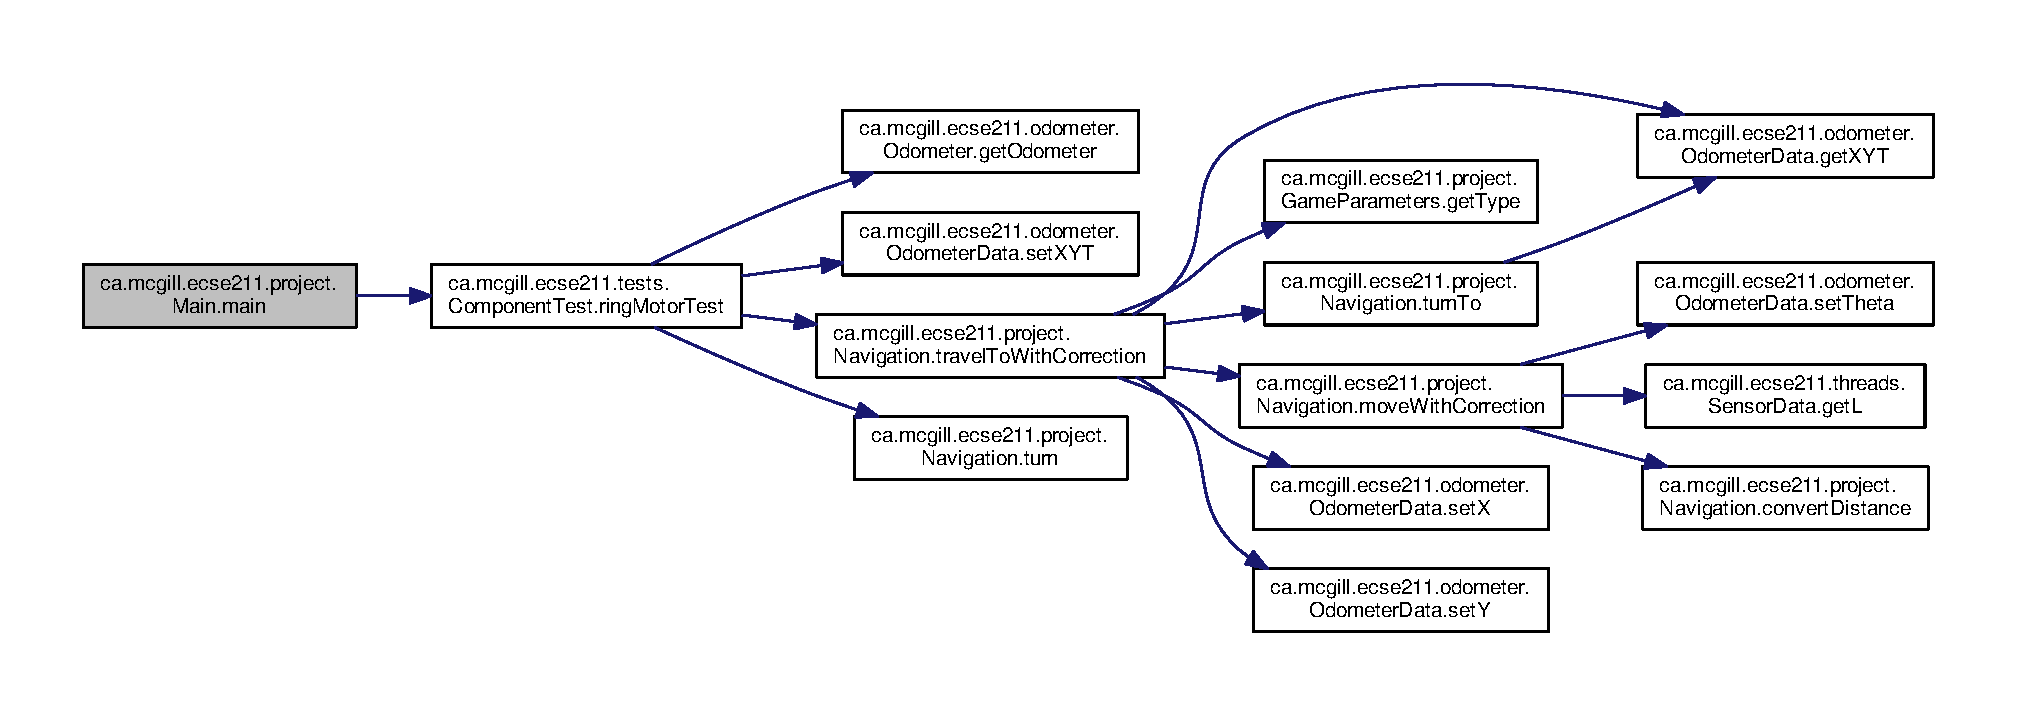
\includegraphics[width=350pt]{classca_1_1mcgill_1_1ecse211_1_1project_1_1_main_af681b5dc675c13ed284071cc135f5fd3_cgraph}
\end{center}
\end{figure}


\subsection{Member Data Documentation}
\mbox{\Hypertarget{classca_1_1mcgill_1_1ecse211_1_1project_1_1_main_af6f7b8fffddcf855f74fe128d2e23ea1}\label{classca_1_1mcgill_1_1ecse211_1_1project_1_1_main_af6f7b8fffddcf855f74fe128d2e23ea1}} 
\index{ca\+::mcgill\+::ecse211\+::project\+::\+Main@{ca\+::mcgill\+::ecse211\+::project\+::\+Main}!test@{test}}
\index{test@{test}!ca\+::mcgill\+::ecse211\+::project\+::\+Main@{ca\+::mcgill\+::ecse211\+::project\+::\+Main}}
\subsubsection{\texorpdfstring{test}{test}}
{\footnotesize\ttfamily boolean ca.\+mcgill.\+ecse211.\+project.\+Main.\+test = true\hspace{0.3cm}{\ttfamily [static]}}

This variable decides whether or not to enable our tests 

Definition at line 21 of file Main.\+java.

\mbox{\Hypertarget{classca_1_1mcgill_1_1ecse211_1_1project_1_1_main_a8dac740460370f76ac0db5dc20824b1f}\label{classca_1_1mcgill_1_1ecse211_1_1project_1_1_main_a8dac740460370f76ac0db5dc20824b1f}} 
\index{ca\+::mcgill\+::ecse211\+::project\+::\+Main@{ca\+::mcgill\+::ecse211\+::project\+::\+Main}!test\+Type@{test\+Type}}
\index{test\+Type@{test\+Type}!ca\+::mcgill\+::ecse211\+::project\+::\+Main@{ca\+::mcgill\+::ecse211\+::project\+::\+Main}}
\subsubsection{\texorpdfstring{test\+Type}{testType}}
{\footnotesize\ttfamily Component\+Test.\+Type ca.\+mcgill.\+ecse211.\+project.\+Main.\+test\+Type = \hyperlink{enumca_1_1mcgill_1_1ecse211_1_1tests_1_1_component_test_1_1_type_ab118eac94e0b37e6871a4c9a788c675e}{Component\+Test.\+Type.\+Ring\+Detection}\hspace{0.3cm}{\ttfamily [static]}}

This variable stores the type of test that we want to perform 

Definition at line 26 of file Main.\+java.



The documentation for this class was generated from the following file\+:\begin{DoxyCompactItemize}
\item 
/home/ccc/\+Final\+Project/src/ca/mcgill/ecse211/project/\hyperlink{_main_8java}{Main.\+java}\end{DoxyCompactItemize}

\hypertarget{classca_1_1mcgill_1_1ecse211_1_1project_1_1_navigation}{}\section{ca.\+mcgill.\+ecse211.\+project.\+Navigation Class Reference}
\label{classca_1_1mcgill_1_1ecse211_1_1project_1_1_navigation}\index{ca.\+mcgill.\+ecse211.\+project.\+Navigation@{ca.\+mcgill.\+ecse211.\+project.\+Navigation}}
\subsection*{Public Member Functions}
\begin{DoxyCompactItemize}
\item 
\hyperlink{classca_1_1mcgill_1_1ecse211_1_1project_1_1_navigation_aaee14b67c392ddd951e3ce21224c3e56}{Navigation} (E\+V3\+Large\+Regulated\+Motor left\+Motor, E\+V3\+Large\+Regulated\+Motor right\+Motor)  throws Odometer\+Exceptions 
\item 
void \hyperlink{classca_1_1mcgill_1_1ecse211_1_1project_1_1_navigation_ab01db7b8a871acd45e7dd16922abc15e}{set\+Slow\+Acc} ()
\item 
double \hyperlink{classca_1_1mcgill_1_1ecse211_1_1project_1_1_navigation_a4376e54162df8f123ca3b52e4fd2f38d}{calculate\+Angle\+To} (double x, double y)
\item 
void \hyperlink{classca_1_1mcgill_1_1ecse211_1_1project_1_1_navigation_a3d8354490a2d8c36090d794c25d33421}{travel\+To} (double x, double y, int speed)
\item 
void \hyperlink{classca_1_1mcgill_1_1ecse211_1_1project_1_1_navigation_ae7230e905494002087416294f12cae6a}{travel\+To\+With\+Correction} (int x, int y, boolean avoid)
\item 
synchronized void \hyperlink{classca_1_1mcgill_1_1ecse211_1_1project_1_1_navigation_a48eeb9ae2da23664421e8da5642054c7}{move\+With\+Correction} (double distance, double theta)
\item 
void \hyperlink{classca_1_1mcgill_1_1ecse211_1_1project_1_1_navigation_afbe677941e2bd44e35452e1eff508ae9}{move\+One\+Tile\+With\+Correction} (double theta)
\item 
synchronized void \hyperlink{classca_1_1mcgill_1_1ecse211_1_1project_1_1_navigation_a3bbe0645f2b3b3d0986b4a707fb5a00c}{turn\+To} (double angle)
\item 
void \hyperlink{classca_1_1mcgill_1_1ecse211_1_1project_1_1_navigation_a4b52e605d3ea2f9bcd9481ae2c69ba39}{go\+Through\+Tunnel} ()  throws Exception 
\item 
void \hyperlink{classca_1_1mcgill_1_1ecse211_1_1project_1_1_navigation_a1a808e665b8dd5b8e79b0580724d239c}{search\+Ring\+Set} (\hyperlink{classca_1_1mcgill_1_1ecse211_1_1project_1_1_ring_searcher}{Ring\+Searcher} searcher, boolean correct, boolean reset)
\item 
void \hyperlink{classca_1_1mcgill_1_1ecse211_1_1project_1_1_navigation_ad74286ad36d333bfaf57661837457b76}{turn} (int angle)
\item 
void \hyperlink{classca_1_1mcgill_1_1ecse211_1_1project_1_1_navigation_a7c66610c5b7496ddb35d342ab2cd3f08}{forward} (int speed, double distance)
\item 
void \hyperlink{classca_1_1mcgill_1_1ecse211_1_1project_1_1_navigation_ae8530d181ffd790ff9dea5eeab54b1a1}{stop} ()
\end{DoxyCompactItemize}
\subsection*{Static Public Member Functions}
\begin{DoxyCompactItemize}
\item 
static int \hyperlink{classca_1_1mcgill_1_1ecse211_1_1project_1_1_navigation_ac9e260bcd619ffa4820d7d0de7ea1c12}{convert\+Distance} (double radius, double distance)
\end{DoxyCompactItemize}


\subsection{Detailed Description}
The Navigator class extends the functionality of the \hyperlink{classca_1_1mcgill_1_1ecse211_1_1project_1_1_navigation}{Navigation} class. It offers an alternative \hyperlink{classca_1_1mcgill_1_1ecse211_1_1project_1_1_navigation_a3d8354490a2d8c36090d794c25d33421}{travel\+To()} method which uses a state machine to implement obstacle avoidance.

The Navigator class does not override any of the methods in \hyperlink{classca_1_1mcgill_1_1ecse211_1_1project_1_1_navigation}{Navigation}. All methods with the same name are overloaded i.\+e. the Navigator version takes different parameters than the \hyperlink{classca_1_1mcgill_1_1ecse211_1_1project_1_1_navigation}{Navigation} version.

This is useful if, for instance, you want to force travel without obstacle detection over small distances. One place where you might want to do this is in the Obstacle\+Avoidance class. Another place is methods that implement specific features for future milestones such as retrieving an object.

\begin{DoxyAuthor}{Author}
Caspar Cedro 

Percy Chen 

Patrick Erath 

Anssam Ghezala 

Susan Matuszewski 

Kamy Moussavi Kafi 
\end{DoxyAuthor}


Definition at line 30 of file Navigation.\+java.



\subsection{Constructor \& Destructor Documentation}
\mbox{\Hypertarget{classca_1_1mcgill_1_1ecse211_1_1project_1_1_navigation_aaee14b67c392ddd951e3ce21224c3e56}\label{classca_1_1mcgill_1_1ecse211_1_1project_1_1_navigation_aaee14b67c392ddd951e3ce21224c3e56}} 
\index{ca\+::mcgill\+::ecse211\+::project\+::\+Navigation@{ca\+::mcgill\+::ecse211\+::project\+::\+Navigation}!Navigation@{Navigation}}
\index{Navigation@{Navigation}!ca\+::mcgill\+::ecse211\+::project\+::\+Navigation@{ca\+::mcgill\+::ecse211\+::project\+::\+Navigation}}
\subsubsection{\texorpdfstring{Navigation()}{Navigation()}}
{\footnotesize\ttfamily ca.\+mcgill.\+ecse211.\+project.\+Navigation.\+Navigation (\begin{DoxyParamCaption}\item[{E\+V3\+Large\+Regulated\+Motor}]{left\+Motor,  }\item[{E\+V3\+Large\+Regulated\+Motor}]{right\+Motor }\end{DoxyParamCaption}) throws \hyperlink{classca_1_1mcgill_1_1ecse211_1_1odometer_1_1_odometer_exceptions}{Odometer\+Exceptions}}

This navigation class constructor sets up our robot to begin navigating a particular map


\begin{DoxyParams}{Parameters}
{\em left\+Motor} & An E\+V3\+Large\+Regulared\+Motor object instance that allows control of the left motor \\
\hline
{\em right\+Motor} & An E\+V3\+Large\+Regulared\+Motor object instance that allows control of the right motor \\
\hline
\end{DoxyParams}


Definition at line 63 of file Navigation.\+java.


\begin{DoxyCode}
64                                 \{
65     this.odometer = Odometer.\hyperlink{classca_1_1mcgill_1_1ecse211_1_1odometer_1_1_odometer_a99171f11e34dea918fa9dd069d721439}{getOdometer}();
66     this.leftMotor = leftMotor;
67     this.rightMotor = rightMotor;
68     this.data = SensorData.\hyperlink{classca_1_1mcgill_1_1ecse211_1_1threads_1_1_sensor_data_a8260aba53b4474ca1275e4ce26157977}{getSensorData}();
69     \textcolor{keywordflow}{for} (EV3LargeRegulatedMotor motor : \textcolor{keyword}{new} EV3LargeRegulatedMotor[] \{this.leftMotor,
70         this.rightMotor\}) \{
71       motor.stop();
72       motor.setAcceleration(Q\_ACCELERATION);
73     \}
74   \}
\end{DoxyCode}
Here is the call graph for this function\+:\nopagebreak
\begin{figure}[H]
\begin{center}
\leavevmode
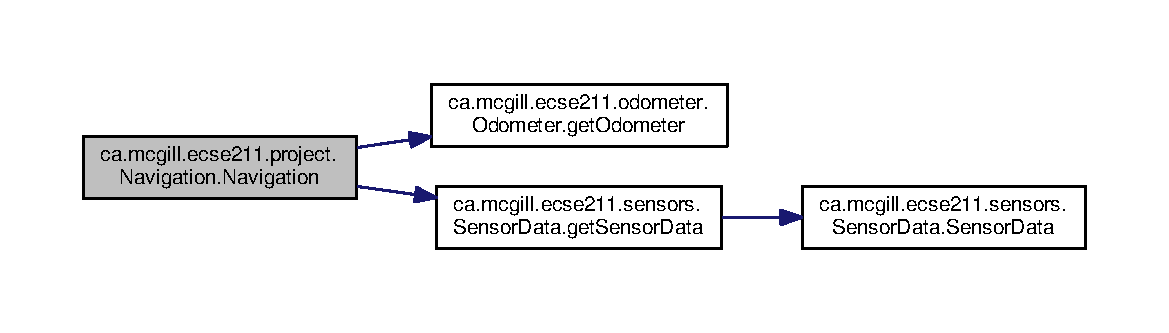
\includegraphics[width=350pt]{classca_1_1mcgill_1_1ecse211_1_1project_1_1_navigation_aaee14b67c392ddd951e3ce21224c3e56_cgraph}
\end{center}
\end{figure}


\subsection{Member Function Documentation}
\mbox{\Hypertarget{classca_1_1mcgill_1_1ecse211_1_1project_1_1_navigation_a4376e54162df8f123ca3b52e4fd2f38d}\label{classca_1_1mcgill_1_1ecse211_1_1project_1_1_navigation_a4376e54162df8f123ca3b52e4fd2f38d}} 
\index{ca\+::mcgill\+::ecse211\+::project\+::\+Navigation@{ca\+::mcgill\+::ecse211\+::project\+::\+Navigation}!calculate\+Angle\+To@{calculate\+Angle\+To}}
\index{calculate\+Angle\+To@{calculate\+Angle\+To}!ca\+::mcgill\+::ecse211\+::project\+::\+Navigation@{ca\+::mcgill\+::ecse211\+::project\+::\+Navigation}}
\subsubsection{\texorpdfstring{calculate\+Angle\+To()}{calculateAngleTo()}}
{\footnotesize\ttfamily double ca.\+mcgill.\+ecse211.\+project.\+Navigation.\+calculate\+Angle\+To (\begin{DoxyParamCaption}\item[{double}]{x,  }\item[{double}]{y }\end{DoxyParamCaption})}

This method calculates the angle necessary for the robot to rotate to face a certain point


\begin{DoxyParams}{Parameters}
{\em x} & The x coordinate of the point to face \\
\hline
{\em y} & The y coordinate of the point to face \\
\hline
\end{DoxyParams}
\begin{DoxyReturn}{Returns}
The rotation angle in degrees 
\end{DoxyReturn}


Definition at line 91 of file Navigation.\+java.


\begin{DoxyCode}
91                                                      \{
92     \textcolor{keywordtype}{double} dX = x - odometer.\hyperlink{classca_1_1mcgill_1_1ecse211_1_1odometer_1_1_odometer_data_a8f40f0264c68f0cbed4fff1723ae7863}{getXYT}()[0];
93     \textcolor{keywordtype}{double} dY = y - odometer.\hyperlink{classca_1_1mcgill_1_1ecse211_1_1odometer_1_1_odometer_data_a8f40f0264c68f0cbed4fff1723ae7863}{getXYT}()[1];
94     \textcolor{keywordtype}{double} theta = Math.atan(dX / dY);
95     \textcolor{keywordflow}{if} (dY < 0 && theta < Math.PI)
96       theta += Math.PI;
97     \textcolor{keywordflow}{return} theta;
98   \}
\end{DoxyCode}
Here is the call graph for this function\+:\nopagebreak
\begin{figure}[H]
\begin{center}
\leavevmode
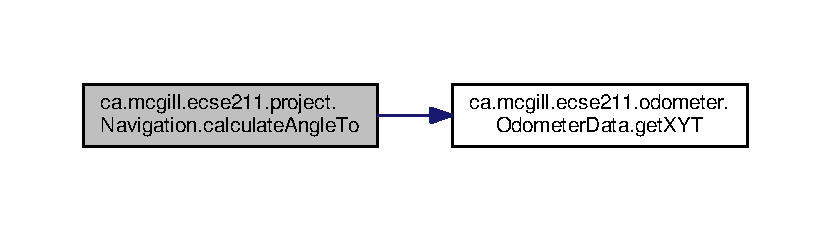
\includegraphics[width=350pt]{classca_1_1mcgill_1_1ecse211_1_1project_1_1_navigation_a4376e54162df8f123ca3b52e4fd2f38d_cgraph}
\end{center}
\end{figure}
Here is the caller graph for this function\+:\nopagebreak
\begin{figure}[H]
\begin{center}
\leavevmode
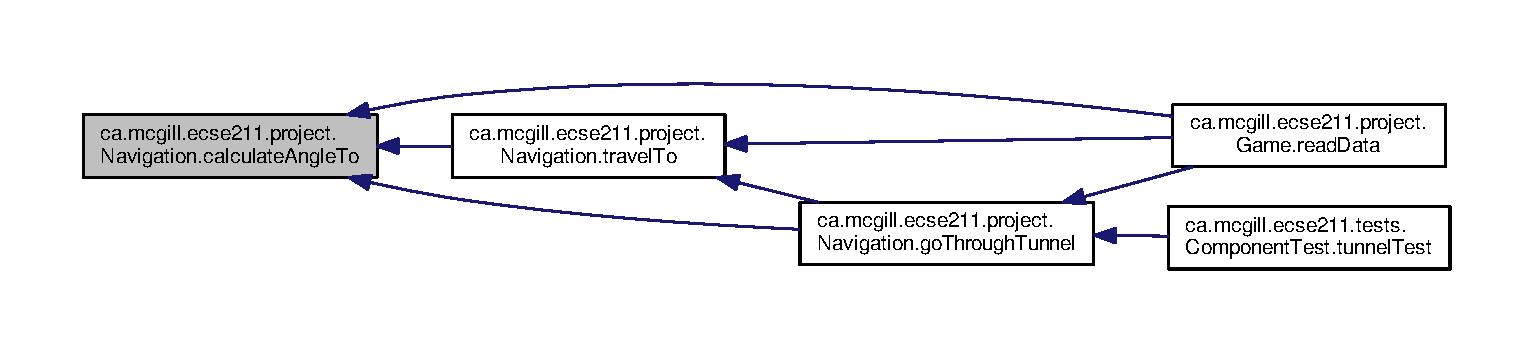
\includegraphics[width=350pt]{classca_1_1mcgill_1_1ecse211_1_1project_1_1_navigation_a4376e54162df8f123ca3b52e4fd2f38d_icgraph}
\end{center}
\end{figure}
\mbox{\Hypertarget{classca_1_1mcgill_1_1ecse211_1_1project_1_1_navigation_ac9e260bcd619ffa4820d7d0de7ea1c12}\label{classca_1_1mcgill_1_1ecse211_1_1project_1_1_navigation_ac9e260bcd619ffa4820d7d0de7ea1c12}} 
\index{ca\+::mcgill\+::ecse211\+::project\+::\+Navigation@{ca\+::mcgill\+::ecse211\+::project\+::\+Navigation}!convert\+Distance@{convert\+Distance}}
\index{convert\+Distance@{convert\+Distance}!ca\+::mcgill\+::ecse211\+::project\+::\+Navigation@{ca\+::mcgill\+::ecse211\+::project\+::\+Navigation}}
\subsubsection{\texorpdfstring{convert\+Distance()}{convertDistance()}}
{\footnotesize\ttfamily static int ca.\+mcgill.\+ecse211.\+project.\+Navigation.\+convert\+Distance (\begin{DoxyParamCaption}\item[{double}]{radius,  }\item[{double}]{distance }\end{DoxyParamCaption})\hspace{0.3cm}{\ttfamily [static]}}

This method converts a distance to the total number of wheel rotations needed to cover that distance.


\begin{DoxyParams}{Parameters}
{\em radius} & The radius of our wheels \\
\hline
{\em distance} & The distance to travel \\
\hline
\end{DoxyParams}
\begin{DoxyReturn}{Returns}
A number of wheel rotations 
\end{DoxyReturn}


Definition at line 653 of file Navigation.\+java.


\begin{DoxyCode}
653                                                                     \{
654     \textcolor{keywordflow}{return} (\textcolor{keywordtype}{int}) ((180.0 * distance) / (Math.PI * radius));
655   \}
\end{DoxyCode}
Here is the caller graph for this function\+:\nopagebreak
\begin{figure}[H]
\begin{center}
\leavevmode
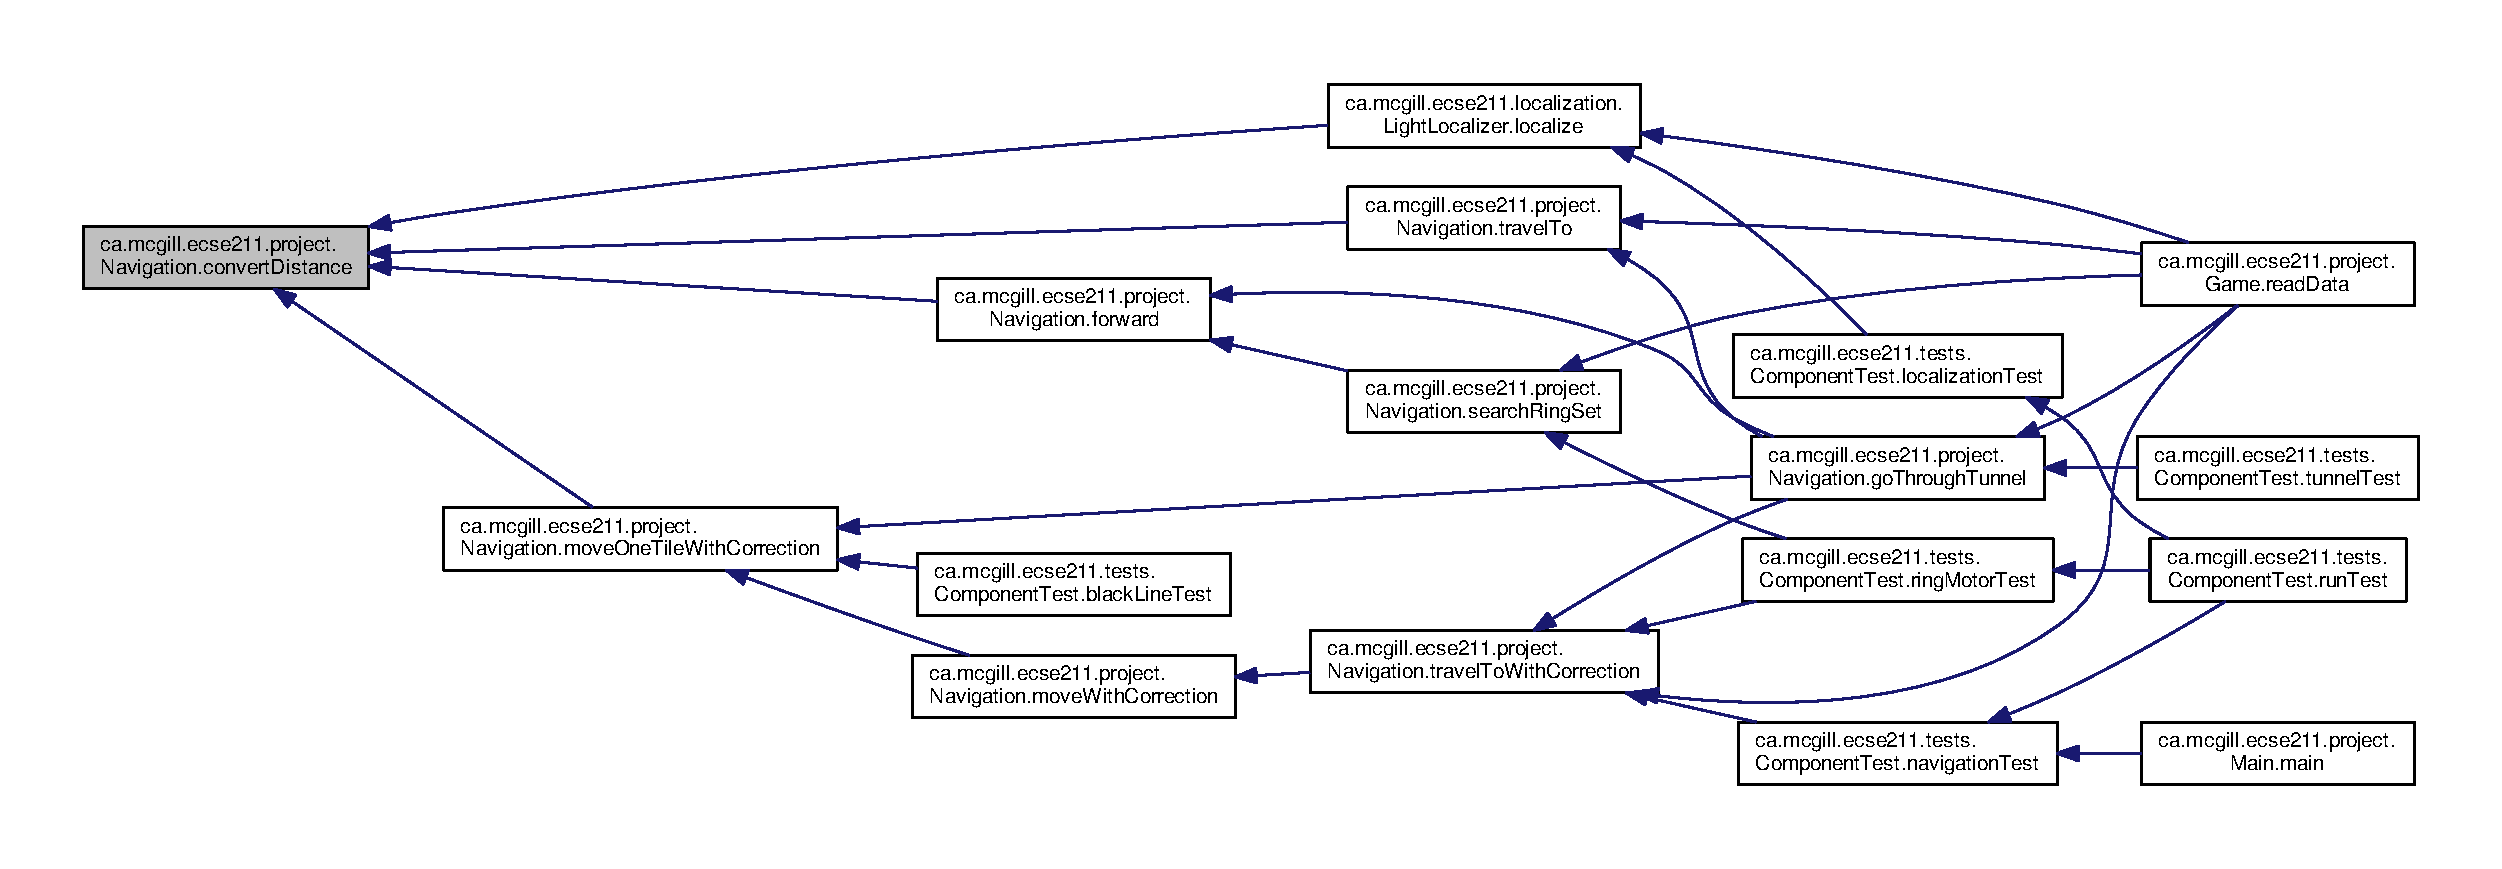
\includegraphics[width=350pt]{classca_1_1mcgill_1_1ecse211_1_1project_1_1_navigation_ac9e260bcd619ffa4820d7d0de7ea1c12_icgraph}
\end{center}
\end{figure}
\mbox{\Hypertarget{classca_1_1mcgill_1_1ecse211_1_1project_1_1_navigation_a7c66610c5b7496ddb35d342ab2cd3f08}\label{classca_1_1mcgill_1_1ecse211_1_1project_1_1_navigation_a7c66610c5b7496ddb35d342ab2cd3f08}} 
\index{ca\+::mcgill\+::ecse211\+::project\+::\+Navigation@{ca\+::mcgill\+::ecse211\+::project\+::\+Navigation}!forward@{forward}}
\index{forward@{forward}!ca\+::mcgill\+::ecse211\+::project\+::\+Navigation@{ca\+::mcgill\+::ecse211\+::project\+::\+Navigation}}
\subsubsection{\texorpdfstring{forward()}{forward()}}
{\footnotesize\ttfamily void ca.\+mcgill.\+ecse211.\+project.\+Navigation.\+forward (\begin{DoxyParamCaption}\item[{int}]{speed,  }\item[{double}]{distance }\end{DoxyParamCaption})}

This method moves our robot forward


\begin{DoxyParams}{Parameters}
{\em speed} & An integer that denotes the speed to rotate our wheels at \\
\hline
{\em distance} & A double that denotes the distance to travel \\
\hline
\end{DoxyParams}


Definition at line 625 of file Navigation.\+java.


\begin{DoxyCode}
625                                                   \{
626     leftMotor.setSpeed(speed);
627     rightMotor.setSpeed(speed);
628     \textcolor{keywordflow}{try} \{
629       Thread.sleep(100);
630     \} \textcolor{keywordflow}{catch} (InterruptedException e) \{
631       e.printStackTrace();
632     \}
633     leftMotor.rotate(\hyperlink{classca_1_1mcgill_1_1ecse211_1_1project_1_1_navigation_ac9e260bcd619ffa4820d7d0de7ea1c12}{convertDistance}(Game.WHEEL\_RAD, distance * Game.TILE), \textcolor{keyword}{true});
634     rightMotor.rotate(\hyperlink{classca_1_1mcgill_1_1ecse211_1_1project_1_1_navigation_ac9e260bcd619ffa4820d7d0de7ea1c12}{convertDistance}(Game.WHEEL\_RAD, distance * Game.TILE), \textcolor{keyword}{false});
635   \}
\end{DoxyCode}
Here is the call graph for this function\+:\nopagebreak
\begin{figure}[H]
\begin{center}
\leavevmode
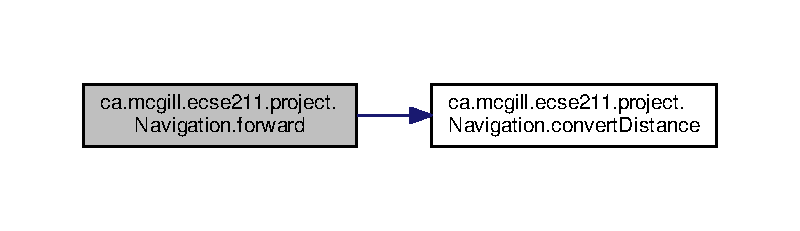
\includegraphics[width=350pt]{classca_1_1mcgill_1_1ecse211_1_1project_1_1_navigation_a7c66610c5b7496ddb35d342ab2cd3f08_cgraph}
\end{center}
\end{figure}
Here is the caller graph for this function\+:\nopagebreak
\begin{figure}[H]
\begin{center}
\leavevmode
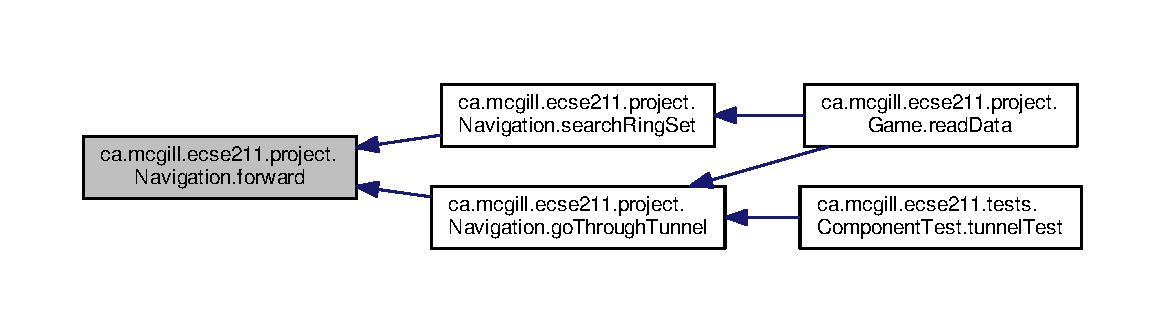
\includegraphics[width=350pt]{classca_1_1mcgill_1_1ecse211_1_1project_1_1_navigation_a7c66610c5b7496ddb35d342ab2cd3f08_icgraph}
\end{center}
\end{figure}
\mbox{\Hypertarget{classca_1_1mcgill_1_1ecse211_1_1project_1_1_navigation_a4b52e605d3ea2f9bcd9481ae2c69ba39}\label{classca_1_1mcgill_1_1ecse211_1_1project_1_1_navigation_a4b52e605d3ea2f9bcd9481ae2c69ba39}} 
\index{ca\+::mcgill\+::ecse211\+::project\+::\+Navigation@{ca\+::mcgill\+::ecse211\+::project\+::\+Navigation}!go\+Through\+Tunnel@{go\+Through\+Tunnel}}
\index{go\+Through\+Tunnel@{go\+Through\+Tunnel}!ca\+::mcgill\+::ecse211\+::project\+::\+Navigation@{ca\+::mcgill\+::ecse211\+::project\+::\+Navigation}}
\subsubsection{\texorpdfstring{go\+Through\+Tunnel()}{goThroughTunnel()}}
{\footnotesize\ttfamily void ca.\+mcgill.\+ecse211.\+project.\+Navigation.\+go\+Through\+Tunnel (\begin{DoxyParamCaption}{ }\end{DoxyParamCaption}) throws Exception}

This method moves our robot through a tunnel by first finding the tunnel based on the lower left and upper right coordinates provided in \hyperlink{enumca_1_1mcgill_1_1ecse211_1_1project_1_1_game_parameters}{Game\+Parameters}, aligning itself with the tunnel and then finally moving through it. the tunnel


\begin{DoxyExceptions}{Exceptions}
{\em Exception} & \\
\hline
\end{DoxyExceptions}


Definition at line 393 of file Navigation.\+java.


\begin{DoxyCode}
393                                                  \{
394     \textcolor{keywordtype}{int} distance = 0;
395     \textcolor{keywordtype}{int}[] ll, ur;
396     \textcolor{comment}{// first use ll and ur coordinate to calculate lr and ul of the tunnel}
397     ll = GameParameters.TN\_LL;
398     ur = GameParameters.TN\_UR;
399     \textcolor{keywordtype}{int}[] lr = \{ll[0], ur[1]\};
400     \textcolor{keywordtype}{int}[] ul = \{ur[0], ll[1]\};
401 
402     \textcolor{comment}{// clone the four points (to make sure we are not modifying the original one)}
403     \textcolor{keywordtype}{int}[][] corners = \{ll.clone(), lr.clone(), ul.clone(), ur.clone()\};
404     ArrayList<int[]> notIn = \textcolor{keyword}{new} ArrayList<int[]>();
405     ArrayList<int[]> points = \textcolor{keyword}{new} ArrayList<int[]>();
406     \textcolor{keywordtype}{double}[] position = odometer.\hyperlink{classca_1_1mcgill_1_1ecse211_1_1odometer_1_1_odometer_data_a8f40f0264c68f0cbed4fff1723ae7863}{getXYT}();
407 
408     \textcolor{comment}{// search for the points that are the same as the current area of the robot}
409     \textcolor{comment}{// these are the entrance of the tunnel, also find the other two points, those}
410     \textcolor{comment}{// are the exit of the tunnel}
411     GameParameters.AreaType type =
412         GameParameters.getType((\textcolor{keywordtype}{int}) Math.round(position[0]), (int) Math.round(position[1]));
413     \textcolor{keywordflow}{for} (\textcolor{keywordtype}{int}[] point : corners) \{
414       \textcolor{keywordflow}{if} (GameParameters.getType(point[0], point[1]) == type) \{
415         points.add(point);
416       \} \textcolor{keywordflow}{else} \{
417         notIn.add(point);
418       \}
419     \}
420 
421     \textcolor{comment}{// Sort the two point at exit by the distance to the destination}
422     \textcolor{keywordflow}{if} (type == GameParameters.AreaType.InStarting) \{
423       Collections.sort(notIn, \textcolor{keyword}{new} GameUtil.RingSetComparator());
424     \} \textcolor{keywordflow}{else} \textcolor{keywordflow}{if} (type == GameParameters.AreaType.Searching) \{
425       Collections.sort(notIn, \textcolor{keyword}{new} GameUtil.StartingComparator());
426     \}
427 
428     \textcolor{comment}{// find the direction and length of the tunnel}
429     \textcolor{comment}{// we know the entrance two points of the tunnel, so this means}
430     \textcolor{comment}{// the two points must have either x or y coordinate identical.}
431     \textcolor{comment}{// that's the direction of the tunnel as well}
432     \textcolor{comment}{// after identify it's direction, we find whether it is positive}
433     \textcolor{comment}{// or negative directed}
434     \textcolor{keywordflow}{if} (points.get(0)[0] == points.get(1)[0]) \{
435       distance = Math.abs(notIn.get(0)[0] - points.get(0)[0]);
436       \textcolor{keywordtype}{int} multi = notIn.get(0)[0] - points.get(0)[0] < 0 ? 1 : -1;
437       travelToTunnelEntrance(points, 0, multi);
438       \textcolor{keywordflow}{for} (\textcolor{keywordtype}{int} i = 0; i < notIn.size(); i++) \{
439         \textcolor{comment}{// this step is to find the nearest two points that we can go two}
440         \textcolor{comment}{// after exit the tunnel}
441         notIn.get(i)[0] = notIn.get(i)[0] - multi * 1;
442       \}
443     \} \textcolor{keywordflow}{else} \{
444       distance = Math.abs(notIn.get(0)[1] - points.get(0)[1]);
445       \textcolor{keywordtype}{int} multi = notIn.get(0)[1] - points.get(0)[1] < 0 ? 1 : -1;
446       travelToTunnelEntrance(points, 1, multi);
447       \textcolor{keywordflow}{for} (\textcolor{keywordtype}{int} i = 0; i < notIn.size(); i++) \{
448         \textcolor{comment}{// this step is to find the nearest two points that we can go two}
449         \textcolor{comment}{// after exit the tunnel}
450         notIn.get(i)[1] = notIn.get(i)[1] - multi * 1;
451       \}
452     \}
453 
454     \textcolor{keywordtype}{double}[] tunnelEnd = GameUtil.average(notIn.get(0), notIn.get(1));
455     \textcolor{keywordtype}{double} angleThoughTunnel = Math.toDegrees(\hyperlink{classca_1_1mcgill_1_1ecse211_1_1project_1_1_navigation_a4376e54162df8f123ca3b52e4fd2f38d}{calculateAngleTo}(tunnelEnd[0], tunnelEnd[1]))
      ;
456     \hyperlink{classca_1_1mcgill_1_1ecse211_1_1project_1_1_navigation_a3bbe0645f2b3b3d0986b4a707fb5a00c}{turnTo}(angleThoughTunnel);
457 
458     \textcolor{comment}{// goback To correct}
459     moveBackWithCorrection();
460 
461     \textcolor{comment}{// turn left -5 to correct the effect of the weight}
462     \hyperlink{classca_1_1mcgill_1_1ecse211_1_1project_1_1_navigation_a7c66610c5b7496ddb35d342ab2cd3f08}{forward}(TUNNEL\_SPEED, 0.5);
463     \hyperlink{classca_1_1mcgill_1_1ecse211_1_1project_1_1_navigation_ad74286ad36d333bfaf57661837457b76}{turn}(TUNNEL\_CORRECTION);
464     \textcolor{keywordflow}{if} (distance == 1) \{
465       \hyperlink{classca_1_1mcgill_1_1ecse211_1_1project_1_1_navigation_a7c66610c5b7496ddb35d342ab2cd3f08}{forward}(TUNNEL\_SPEED, distance + 1);
466     \} \textcolor{keywordflow}{else} \{
467 
468       \hyperlink{classca_1_1mcgill_1_1ecse211_1_1project_1_1_navigation_a7c66610c5b7496ddb35d342ab2cd3f08}{forward}(TUNNEL\_SPEED, distance + 1);
469     \}
470 
471     odometer.\hyperlink{classca_1_1mcgill_1_1ecse211_1_1odometer_1_1_odometer_data_a419b8f07c2c5374411c8e62298e9a402}{setTheta}(angleThoughTunnel);
472     \textcolor{comment}{// leftMotor.setAcceleration(N\_ACCELERATION);}
473     \textcolor{comment}{// rightMotor.setAcceleration(N\_ACCELERATION);}
474     \textcolor{comment}{// // rotate additional sensor distances to make sure the sensor will not on the balck line}
475     \textcolor{comment}{// leftMotor.rotate(convertDistance(Game.WHEEL\_RAD, 2*Game.SEN\_DIS), true);}
476     \textcolor{comment}{// rightMotor.rotate(convertDistance(Game.WHEEL\_RAD, 2*Game.SEN\_DIS), false);}
477     this.\hyperlink{classca_1_1mcgill_1_1ecse211_1_1project_1_1_navigation_afbe677941e2bd44e35452e1eff508ae9}{moveOneTileWithCorrection}(angleThoughTunnel);
478     \textcolor{keywordtype}{double}[] after = GameUtil.average(notIn.get(0), notIn.get(1));
479     odometer.\hyperlink{classca_1_1mcgill_1_1ecse211_1_1odometer_1_1_odometer_data_a2911d7215e47f3064defe016b46bfeef}{setX}(after[0]);
480     odometer.\hyperlink{classca_1_1mcgill_1_1ecse211_1_1odometer_1_1_odometer_data_a82986438cd462e66520bc62bb4bd2b75}{setY}(after[1]);
481     \textcolor{comment}{// go to the nearest safe point near tunnel}
482     \textcolor{keywordflow}{for} (\textcolor{keywordtype}{int}[] p : notIn) \{
483       \textcolor{keywordflow}{if} (GameUtil.isSafe(p)) \{
484         \textcolor{keywordtype}{double} toPointAngle = Math.toDegrees(\hyperlink{classca_1_1mcgill_1_1ecse211_1_1project_1_1_navigation_a4376e54162df8f123ca3b52e4fd2f38d}{calculateAngleTo}(p[0], p[1]));
485         \hyperlink{classca_1_1mcgill_1_1ecse211_1_1project_1_1_navigation_a3bbe0645f2b3b3d0986b4a707fb5a00c}{turnTo}(toPointAngle);
486         this.\hyperlink{classca_1_1mcgill_1_1ecse211_1_1project_1_1_navigation_afbe677941e2bd44e35452e1eff508ae9}{moveOneTileWithCorrection}(toPointAngle);
487         odometer.\hyperlink{classca_1_1mcgill_1_1ecse211_1_1odometer_1_1_odometer_data_a2911d7215e47f3064defe016b46bfeef}{setX}(p[0]);
488         odometer.\hyperlink{classca_1_1mcgill_1_1ecse211_1_1odometer_1_1_odometer_data_a82986438cd462e66520bc62bb4bd2b75}{setY}(p[1]);
489         \textcolor{keywordflow}{break};
490       \}
491     \}
492   \}
\end{DoxyCode}
Here is the call graph for this function\+:\nopagebreak
\begin{figure}[H]
\begin{center}
\leavevmode
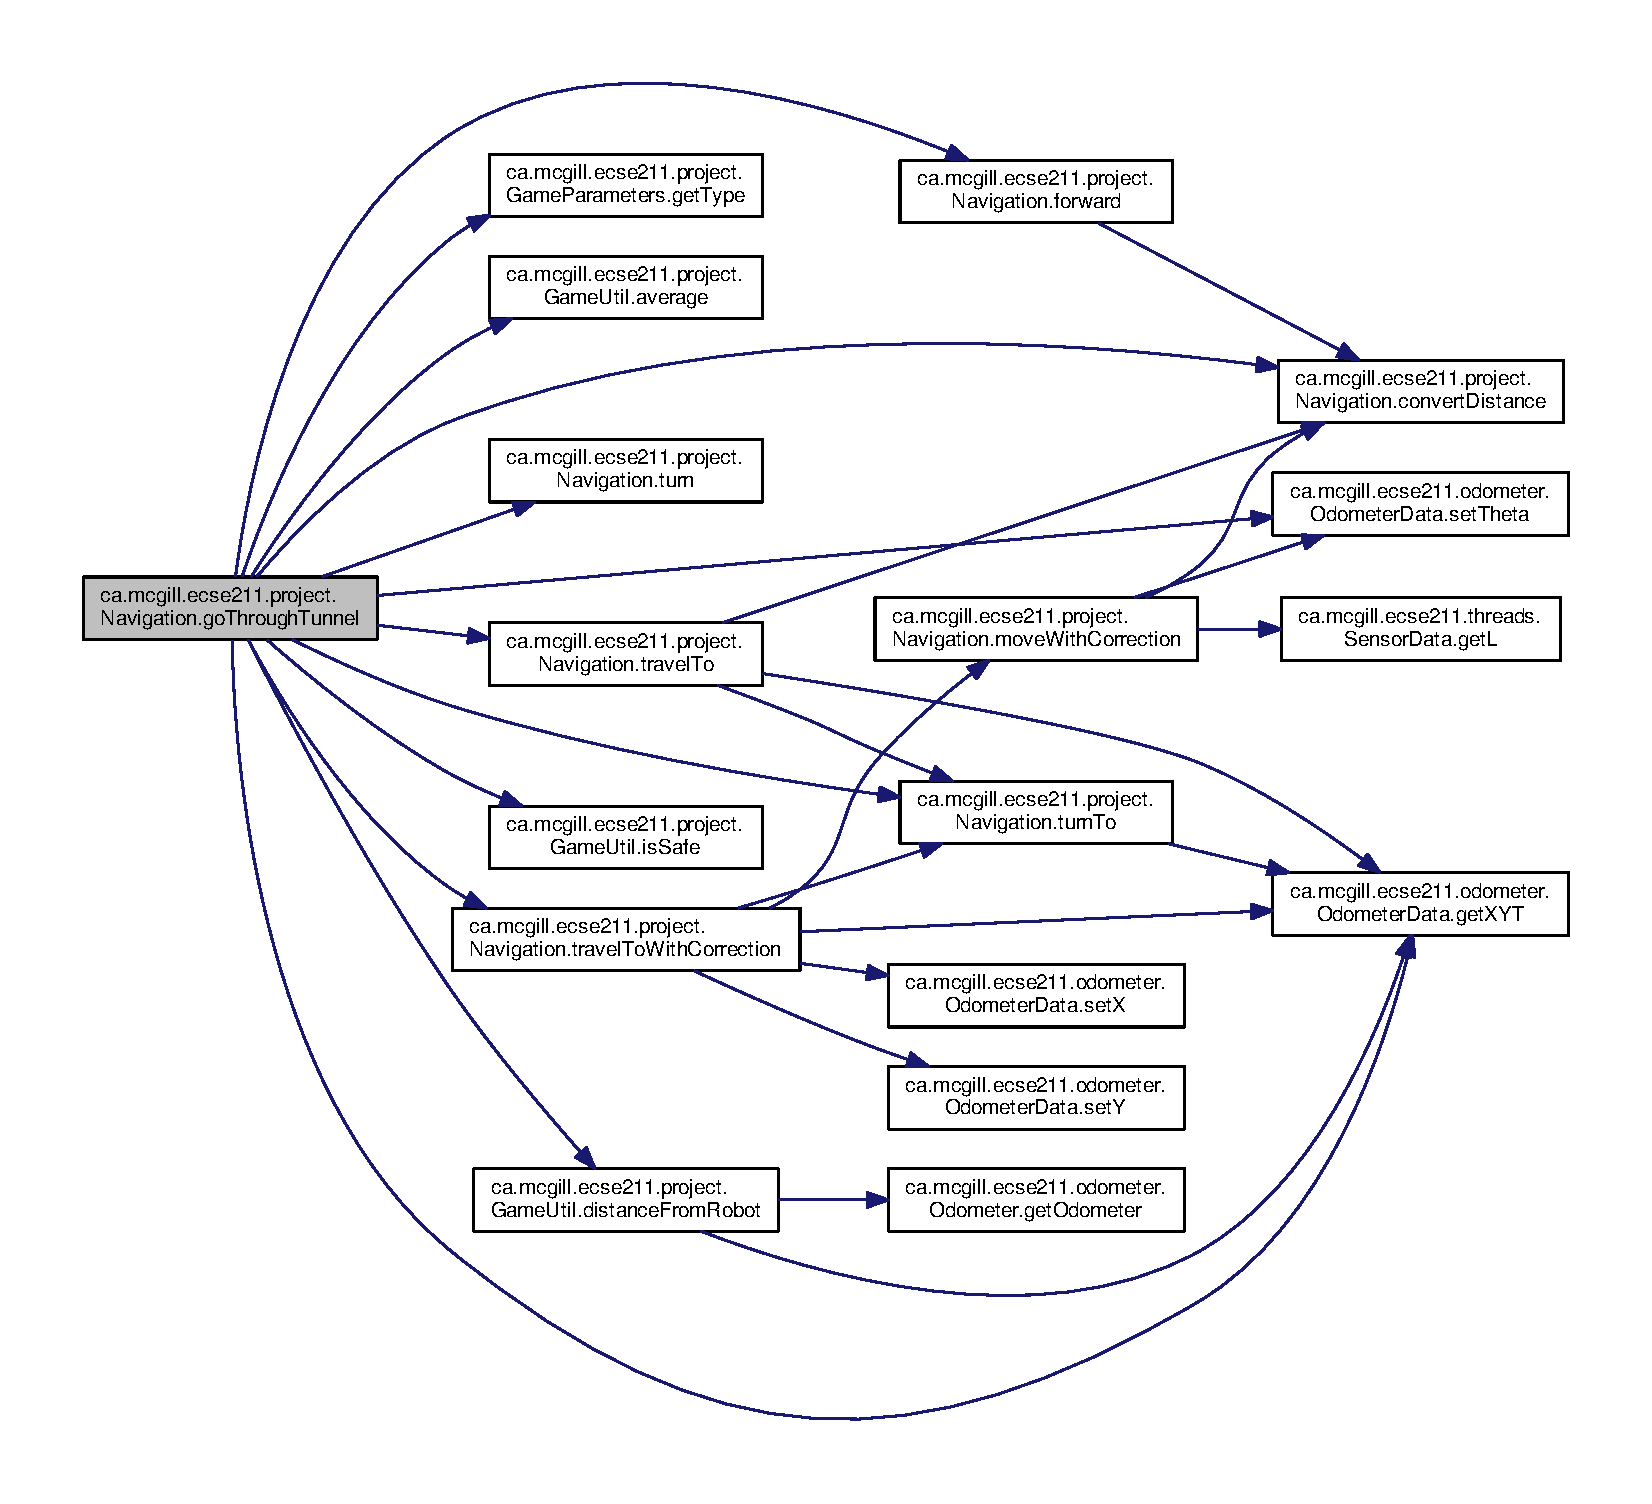
\includegraphics[width=350pt]{classca_1_1mcgill_1_1ecse211_1_1project_1_1_navigation_a4b52e605d3ea2f9bcd9481ae2c69ba39_cgraph}
\end{center}
\end{figure}
Here is the caller graph for this function\+:\nopagebreak
\begin{figure}[H]
\begin{center}
\leavevmode
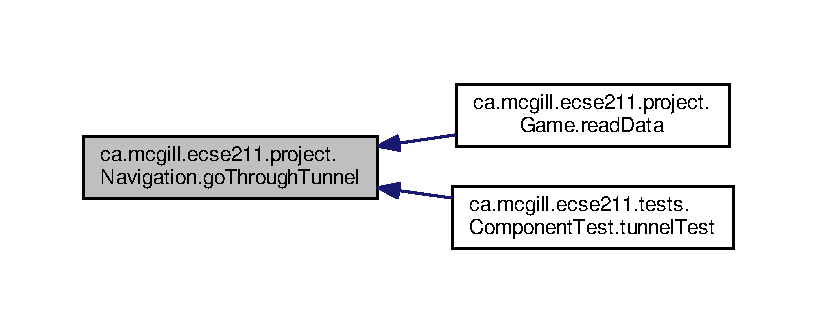
\includegraphics[width=350pt]{classca_1_1mcgill_1_1ecse211_1_1project_1_1_navigation_a4b52e605d3ea2f9bcd9481ae2c69ba39_icgraph}
\end{center}
\end{figure}
\mbox{\Hypertarget{classca_1_1mcgill_1_1ecse211_1_1project_1_1_navigation_afbe677941e2bd44e35452e1eff508ae9}\label{classca_1_1mcgill_1_1ecse211_1_1project_1_1_navigation_afbe677941e2bd44e35452e1eff508ae9}} 
\index{ca\+::mcgill\+::ecse211\+::project\+::\+Navigation@{ca\+::mcgill\+::ecse211\+::project\+::\+Navigation}!move\+One\+Tile\+With\+Correction@{move\+One\+Tile\+With\+Correction}}
\index{move\+One\+Tile\+With\+Correction@{move\+One\+Tile\+With\+Correction}!ca\+::mcgill\+::ecse211\+::project\+::\+Navigation@{ca\+::mcgill\+::ecse211\+::project\+::\+Navigation}}
\subsubsection{\texorpdfstring{move\+One\+Tile\+With\+Correction()}{moveOneTileWithCorrection()}}
{\footnotesize\ttfamily void ca.\+mcgill.\+ecse211.\+project.\+Navigation.\+move\+One\+Tile\+With\+Correction (\begin{DoxyParamCaption}\item[{double}]{theta }\end{DoxyParamCaption})}

This method moves the robot one tile until it detects a black line


\begin{DoxyParams}{Parameters}
{\em theta} & The angle to be corrected to upon crossing a tile \\
\hline
\end{DoxyParams}


Definition at line 258 of file Navigation.\+java.


\begin{DoxyCode}
258                                                       \{
259     \textcolor{comment}{// leftMotor.setAcceleration(N\_ACCELERATION);}
260     \textcolor{comment}{// rightMotor.setAcceleration(N\_ACCELERATION);}
261     leftMotor.setSpeed(FORWARD\_SPEED);
262     rightMotor.setSpeed(FORWARD\_SPEED);
263     leftMotor.forward();
264     rightMotor.forward();
265     moveUntilLineDetection(\textcolor{keyword}{true});
266     odometer.\hyperlink{classca_1_1mcgill_1_1ecse211_1_1odometer_1_1_odometer_data_a419b8f07c2c5374411c8e62298e9a402}{setTheta}(theta);
267   \}
\end{DoxyCode}
Here is the call graph for this function\+:\nopagebreak
\begin{figure}[H]
\begin{center}
\leavevmode
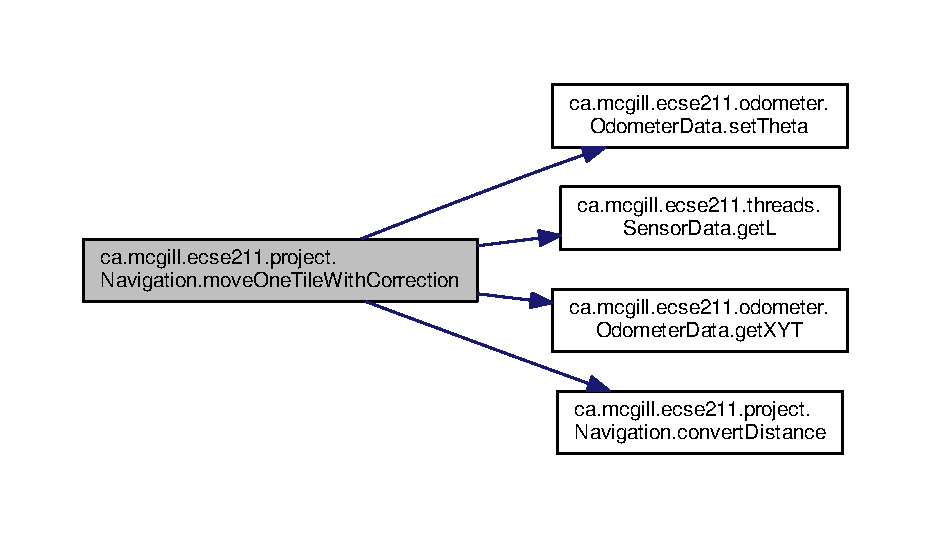
\includegraphics[width=350pt]{classca_1_1mcgill_1_1ecse211_1_1project_1_1_navigation_afbe677941e2bd44e35452e1eff508ae9_cgraph}
\end{center}
\end{figure}
Here is the caller graph for this function\+:\nopagebreak
\begin{figure}[H]
\begin{center}
\leavevmode
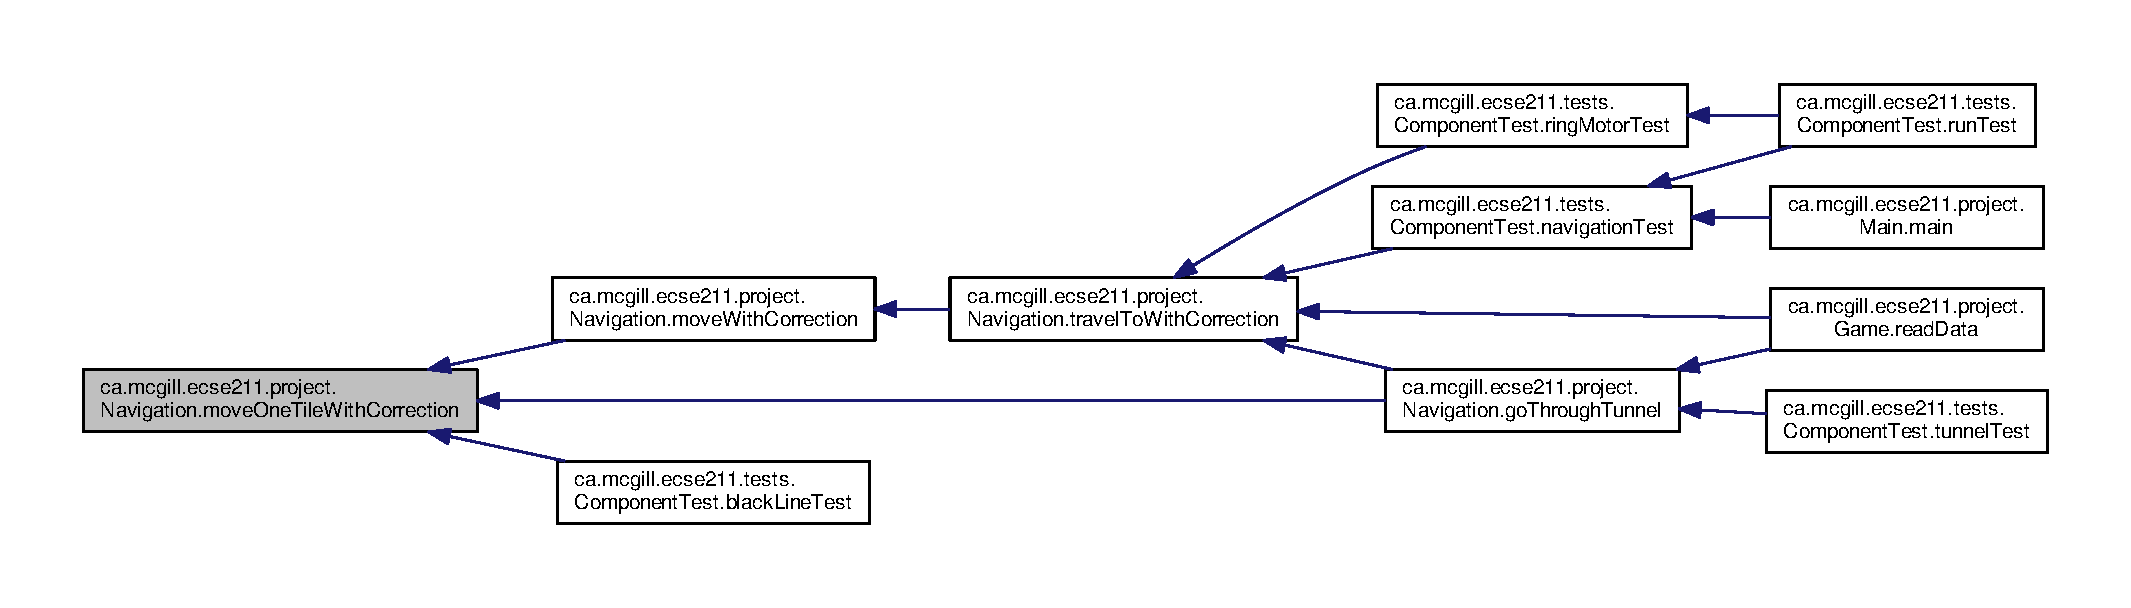
\includegraphics[width=350pt]{classca_1_1mcgill_1_1ecse211_1_1project_1_1_navigation_afbe677941e2bd44e35452e1eff508ae9_icgraph}
\end{center}
\end{figure}
\mbox{\Hypertarget{classca_1_1mcgill_1_1ecse211_1_1project_1_1_navigation_a48eeb9ae2da23664421e8da5642054c7}\label{classca_1_1mcgill_1_1ecse211_1_1project_1_1_navigation_a48eeb9ae2da23664421e8da5642054c7}} 
\index{ca\+::mcgill\+::ecse211\+::project\+::\+Navigation@{ca\+::mcgill\+::ecse211\+::project\+::\+Navigation}!move\+With\+Correction@{move\+With\+Correction}}
\index{move\+With\+Correction@{move\+With\+Correction}!ca\+::mcgill\+::ecse211\+::project\+::\+Navigation@{ca\+::mcgill\+::ecse211\+::project\+::\+Navigation}}
\subsubsection{\texorpdfstring{move\+With\+Correction()}{moveWithCorrection()}}
{\footnotesize\ttfamily synchronized void ca.\+mcgill.\+ecse211.\+project.\+Navigation.\+move\+With\+Correction (\begin{DoxyParamCaption}\item[{double}]{distance,  }\item[{double}]{theta }\end{DoxyParamCaption})}

This method moves our robot a certain distance with corrections if required.


\begin{DoxyParams}{Parameters}
{\em distance} & The distance our robot is to travel \\
\hline
{\em theta} & The angle to be corrected to upon crossing a tile \\
\hline
\end{DoxyParams}


Definition at line 229 of file Navigation.\+java.


\begin{DoxyCode}
229                                                                              \{
230     leftMotor.setSpeed(FORWARD\_SPEED);
231     rightMotor.setSpeed(FORWARD\_SPEED);
232 
233     \textcolor{comment}{// correct error of the distance}
234     \textcolor{keywordtype}{int} tiles = Math.abs((\textcolor{keywordtype}{int}) Math.round(distance));
235     \textcolor{keywordflow}{for} (\textcolor{keywordtype}{int} i = 0; i < tiles; i++) \{
236       \hyperlink{classca_1_1mcgill_1_1ecse211_1_1project_1_1_navigation_afbe677941e2bd44e35452e1eff508ae9}{moveOneTileWithCorrection}(theta);
237     \}
238   \}
\end{DoxyCode}
Here is the call graph for this function\+:\nopagebreak
\begin{figure}[H]
\begin{center}
\leavevmode
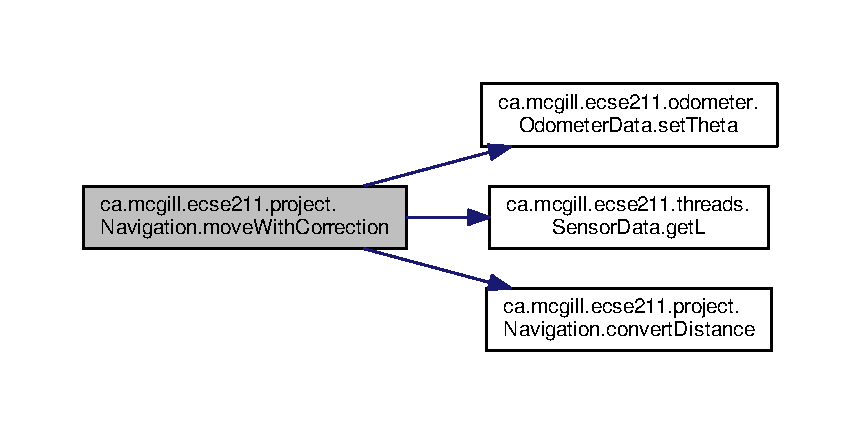
\includegraphics[width=350pt]{classca_1_1mcgill_1_1ecse211_1_1project_1_1_navigation_a48eeb9ae2da23664421e8da5642054c7_cgraph}
\end{center}
\end{figure}
Here is the caller graph for this function\+:\nopagebreak
\begin{figure}[H]
\begin{center}
\leavevmode
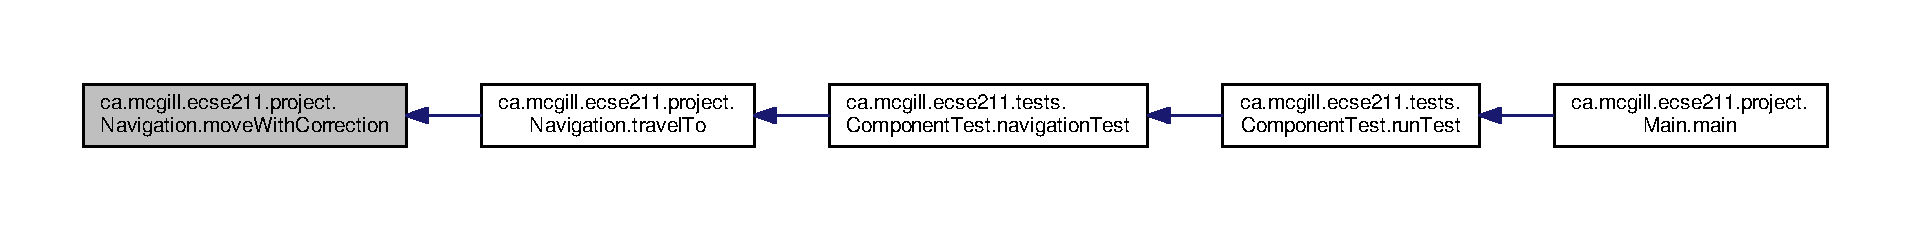
\includegraphics[width=350pt]{classca_1_1mcgill_1_1ecse211_1_1project_1_1_navigation_a48eeb9ae2da23664421e8da5642054c7_icgraph}
\end{center}
\end{figure}
\mbox{\Hypertarget{classca_1_1mcgill_1_1ecse211_1_1project_1_1_navigation_a1a808e665b8dd5b8e79b0580724d239c}\label{classca_1_1mcgill_1_1ecse211_1_1project_1_1_navigation_a1a808e665b8dd5b8e79b0580724d239c}} 
\index{ca\+::mcgill\+::ecse211\+::project\+::\+Navigation@{ca\+::mcgill\+::ecse211\+::project\+::\+Navigation}!search\+Ring\+Set@{search\+Ring\+Set}}
\index{search\+Ring\+Set@{search\+Ring\+Set}!ca\+::mcgill\+::ecse211\+::project\+::\+Navigation@{ca\+::mcgill\+::ecse211\+::project\+::\+Navigation}}
\subsubsection{\texorpdfstring{search\+Ring\+Set()}{searchRingSet()}}
{\footnotesize\ttfamily void ca.\+mcgill.\+ecse211.\+project.\+Navigation.\+search\+Ring\+Set (\begin{DoxyParamCaption}\item[{\hyperlink{classca_1_1mcgill_1_1ecse211_1_1project_1_1_ring_searcher}{Ring\+Searcher}}]{searcher,  }\item[{boolean}]{correct,  }\item[{boolean}]{reset }\end{DoxyParamCaption})}

This method moves our robot towards a ring set by noting ultrasonic sensor readings


\begin{DoxyParams}{Parameters}
{\em searcher} & A \hyperlink{classca_1_1mcgill_1_1ecse211_1_1project_1_1_ring_searcher}{Ring\+Searcher} object instance to detect ring colors and navigate around a ring set \\
\hline
{\em correct} & A boolean that decides whether to correct our position when searching for a ring \\
\hline
{\em reset} & A boolean that decides whether to rotate the rod motor to its original position \\
\hline
\end{DoxyParams}


Definition at line 537 of file Navigation.\+java.


\begin{DoxyCode}
537                                                                                    \{
538     \textcolor{comment}{// Go backward to detect the line and correct the rotation}
539     \textcolor{comment}{// leftMotor.setAcceleration(N\_ACCELERATION);}
540     \textcolor{comment}{// rightMotor.setAcceleration(N\_ACCELERATION);}
541     leftMotor.setSpeed(FORWARD\_SPEED);
542     rightMotor.setSpeed(FORWARD\_SPEED);
543     \textcolor{keywordflow}{try} \{
544       Thread.sleep(100);
545     \} \textcolor{keywordflow}{catch} (InterruptedException e) \{
546       e.printStackTrace();
547     \}
548     \textcolor{keywordtype}{double} theta = odometer.\hyperlink{classca_1_1mcgill_1_1ecse211_1_1odometer_1_1_odometer_data_a8f40f0264c68f0cbed4fff1723ae7863}{getXYT}()[2];
549 
550     \textcolor{comment}{// if we do correction, we need to forward more (for the sensor distance)}
551     \textcolor{keywordflow}{if} (correct) \{
552       leftMotor.backward();
553       rightMotor.backward();
554       moveUntilLineDetection(\textcolor{keyword}{true});
555       \textcolor{comment}{// Forward for 3 cm (approach the ring set)}
556       \textcolor{comment}{// forward(FORWARD\_SPEED, 2.5 / Game.TILE);}
557     \} \textcolor{keywordflow}{else} \{
558       \textcolor{comment}{// forward(FORWARD\_SPEED, 2 / Game.TILE);}
559     \}
560     searcher.prepareRetrieve();
561     \textcolor{comment}{// rotate a little to the left to make sure that the sensor can detect the ring}
562     \textcolor{comment}{// detect the ring color and beep based on the color}
563     searcher.search(-165);
564     \textcolor{keywordflow}{if} (correct) \{
565       \hyperlink{classca_1_1mcgill_1_1ecse211_1_1project_1_1_navigation_a7c66610c5b7496ddb35d342ab2cd3f08}{forward}(FORWARD\_SPEED, 2.8 / Game.TILE);
566     \} \textcolor{keywordflow}{else} \{
567       \hyperlink{classca_1_1mcgill_1_1ecse211_1_1project_1_1_navigation_a7c66610c5b7496ddb35d342ab2cd3f08}{forward}(FORWARD\_SPEED, 3.8 / Game.TILE);
568     \}
569     searcher.detectColor();
570     searcher.search(-190);
571     searcher.detectColor();
572 
573     \textcolor{comment}{// rotate back}
574     \textcolor{comment}{// leftMotor.rotate(-LEFT\_MOTOR\_RING\_COR, false);}
575     \textcolor{comment}{// prepare for retrieving the ring}
576     searcher.finishSearch();
577 
578     rightMotor.rotate(-40, \textcolor{keyword}{false});
579     searcher.safeRod();
580     \textcolor{keywordflow}{if} (correct) \{
581       \hyperlink{classca_1_1mcgill_1_1ecse211_1_1project_1_1_navigation_a7c66610c5b7496ddb35d342ab2cd3f08}{forward}(FORWARD\_SPEED, 3.7 / Game.TILE);
582     \} \textcolor{keywordflow}{else} \{
583       \hyperlink{classca_1_1mcgill_1_1ecse211_1_1project_1_1_navigation_a7c66610c5b7496ddb35d342ab2cd3f08}{forward}(FORWARD\_SPEED, 2.7 / Game.TILE);
584     \}
585     \textcolor{comment}{// go back to original position}
586     rightMotor.rotate(70, \textcolor{keyword}{false});
587     searcher.retrieveRing();
588     \textcolor{comment}{// rotate the right motor to behind a little to make sure we can put the rod behind the ring}
589     \textcolor{comment}{// rightMotor.rotate(RIGHT\_MOTOR\_RING\_COR, false);}
590 
591     \textcolor{comment}{// go to the position where ring can be retrieved}
592 
593     \textcolor{comment}{// rotate a little to the left to make sure not influence the other ring}
594     rightMotor.rotate(-70, \textcolor{keyword}{false});
595 
596     \hyperlink{classca_1_1mcgill_1_1ecse211_1_1project_1_1_navigation_a7c66610c5b7496ddb35d342ab2cd3f08}{forward}(FORWARD\_SPEED, -6.5 / Game.TILE);
597     \textcolor{comment}{// go back to original position}
598     rightMotor.rotate(40 + 30, \textcolor{keyword}{false});
599 
600     \textcolor{comment}{// if (correct) \{}
601     \textcolor{comment}{// forward(FORWARD\_SPEED, -6.5 / Game.TILE);}
602     \textcolor{comment}{// \} else \{}
603     \textcolor{comment}{// forward(FORWARD\_SPEED, -6 / Game.TILE);}
604     \textcolor{comment}{// \}}
605     \textcolor{comment}{// if (reset)}
606     \textcolor{comment}{// searcher.resetRodMotor();}
607   \}
\end{DoxyCode}
Here is the call graph for this function\+:\nopagebreak
\begin{figure}[H]
\begin{center}
\leavevmode
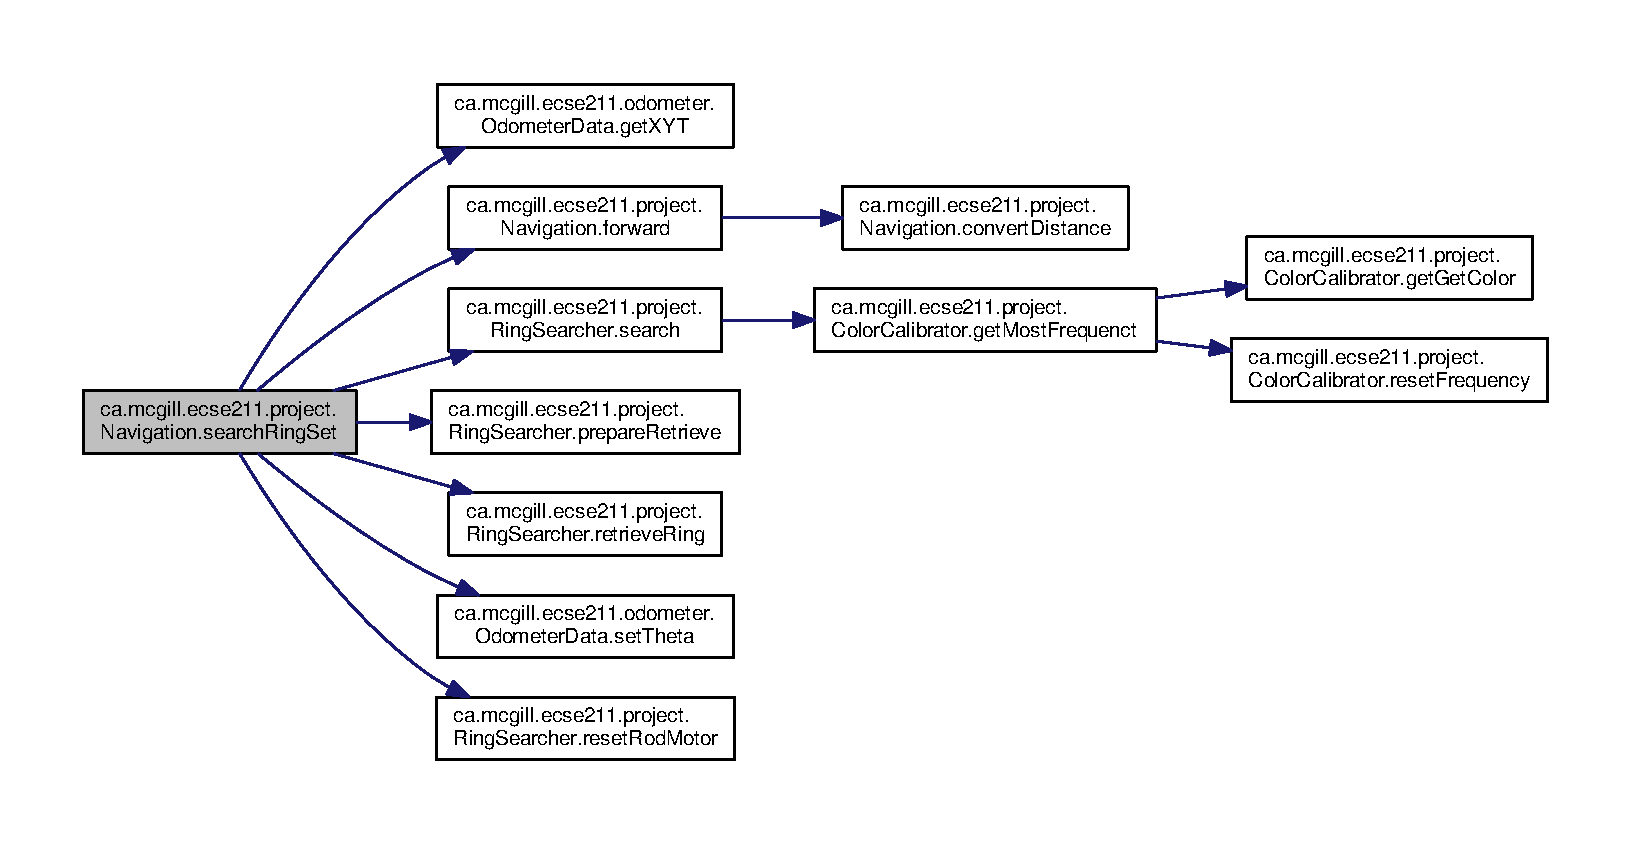
\includegraphics[width=350pt]{classca_1_1mcgill_1_1ecse211_1_1project_1_1_navigation_a1a808e665b8dd5b8e79b0580724d239c_cgraph}
\end{center}
\end{figure}
Here is the caller graph for this function\+:\nopagebreak
\begin{figure}[H]
\begin{center}
\leavevmode
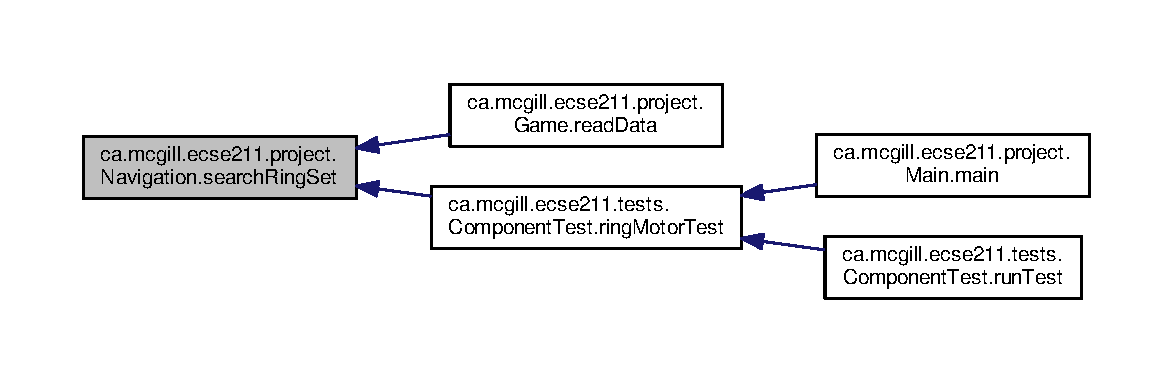
\includegraphics[width=350pt]{classca_1_1mcgill_1_1ecse211_1_1project_1_1_navigation_a1a808e665b8dd5b8e79b0580724d239c_icgraph}
\end{center}
\end{figure}
\mbox{\Hypertarget{classca_1_1mcgill_1_1ecse211_1_1project_1_1_navigation_ab01db7b8a871acd45e7dd16922abc15e}\label{classca_1_1mcgill_1_1ecse211_1_1project_1_1_navigation_ab01db7b8a871acd45e7dd16922abc15e}} 
\index{ca\+::mcgill\+::ecse211\+::project\+::\+Navigation@{ca\+::mcgill\+::ecse211\+::project\+::\+Navigation}!set\+Slow\+Acc@{set\+Slow\+Acc}}
\index{set\+Slow\+Acc@{set\+Slow\+Acc}!ca\+::mcgill\+::ecse211\+::project\+::\+Navigation@{ca\+::mcgill\+::ecse211\+::project\+::\+Navigation}}
\subsubsection{\texorpdfstring{set\+Slow\+Acc()}{setSlowAcc()}}
{\footnotesize\ttfamily void ca.\+mcgill.\+ecse211.\+project.\+Navigation.\+set\+Slow\+Acc (\begin{DoxyParamCaption}{ }\end{DoxyParamCaption})}

This method sets the motor acceleration speed to a lower threshold value 

Definition at line 79 of file Navigation.\+java.


\begin{DoxyCode}
79                            \{
80     leftMotor.setAcceleration(N\_ACCELERATION);
81     rightMotor.setAcceleration(N\_ACCELERATION);
82   \}
\end{DoxyCode}
Here is the caller graph for this function\+:\nopagebreak
\begin{figure}[H]
\begin{center}
\leavevmode
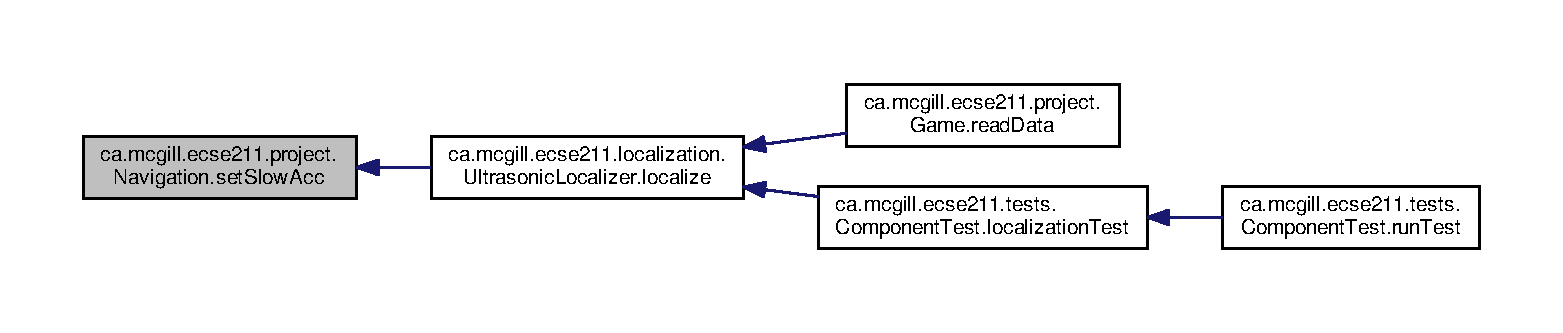
\includegraphics[width=350pt]{classca_1_1mcgill_1_1ecse211_1_1project_1_1_navigation_ab01db7b8a871acd45e7dd16922abc15e_icgraph}
\end{center}
\end{figure}
\mbox{\Hypertarget{classca_1_1mcgill_1_1ecse211_1_1project_1_1_navigation_ae8530d181ffd790ff9dea5eeab54b1a1}\label{classca_1_1mcgill_1_1ecse211_1_1project_1_1_navigation_ae8530d181ffd790ff9dea5eeab54b1a1}} 
\index{ca\+::mcgill\+::ecse211\+::project\+::\+Navigation@{ca\+::mcgill\+::ecse211\+::project\+::\+Navigation}!stop@{stop}}
\index{stop@{stop}!ca\+::mcgill\+::ecse211\+::project\+::\+Navigation@{ca\+::mcgill\+::ecse211\+::project\+::\+Navigation}}
\subsubsection{\texorpdfstring{stop()}{stop()}}
{\footnotesize\ttfamily void ca.\+mcgill.\+ecse211.\+project.\+Navigation.\+stop (\begin{DoxyParamCaption}{ }\end{DoxyParamCaption})}

This method stops both motors 

Definition at line 640 of file Navigation.\+java.


\begin{DoxyCode}
640                      \{
641     leftMotor.stop(\textcolor{keyword}{true});
642     rightMotor.stop(\textcolor{keyword}{false});
643   \}
\end{DoxyCode}
\mbox{\Hypertarget{classca_1_1mcgill_1_1ecse211_1_1project_1_1_navigation_a3d8354490a2d8c36090d794c25d33421}\label{classca_1_1mcgill_1_1ecse211_1_1project_1_1_navigation_a3d8354490a2d8c36090d794c25d33421}} 
\index{ca\+::mcgill\+::ecse211\+::project\+::\+Navigation@{ca\+::mcgill\+::ecse211\+::project\+::\+Navigation}!travel\+To@{travel\+To}}
\index{travel\+To@{travel\+To}!ca\+::mcgill\+::ecse211\+::project\+::\+Navigation@{ca\+::mcgill\+::ecse211\+::project\+::\+Navigation}}
\subsubsection{\texorpdfstring{travel\+To()}{travelTo()}}
{\footnotesize\ttfamily void ca.\+mcgill.\+ecse211.\+project.\+Navigation.\+travel\+To (\begin{DoxyParamCaption}\item[{double}]{x,  }\item[{double}]{y,  }\item[{int}]{speed }\end{DoxyParamCaption})}

This method makes our robot travel to a point by first rotating it and then traversing to the point


\begin{DoxyParams}{Parameters}
{\em x} & The x coordinate of the point to travel to \\
\hline
{\em y} & The y coordinate of the point to travel to \\
\hline
\end{DoxyParams}


Definition at line 107 of file Navigation.\+java.


\begin{DoxyCode}
107                                                       \{
108     \textcolor{keywordtype}{double} dX = x - odometer.\hyperlink{classca_1_1mcgill_1_1ecse211_1_1odometer_1_1_odometer_data_a8f40f0264c68f0cbed4fff1723ae7863}{getXYT}()[0];
109     \textcolor{keywordtype}{double} dY = y - odometer.\hyperlink{classca_1_1mcgill_1_1ecse211_1_1odometer_1_1_odometer_data_a8f40f0264c68f0cbed4fff1723ae7863}{getXYT}()[1];
110     \textcolor{keywordtype}{double} theta = \hyperlink{classca_1_1mcgill_1_1ecse211_1_1project_1_1_navigation_a4376e54162df8f123ca3b52e4fd2f38d}{calculateAngleTo}(x, y);
111 
112     \textcolor{comment}{// Euclidean distance calculation.}
113     \textcolor{keywordtype}{double} distance = Math.sqrt(Math.pow(dX, 2) + Math.pow(dY, 2));
114 
115     \hyperlink{classca_1_1mcgill_1_1ecse211_1_1project_1_1_navigation_a3bbe0645f2b3b3d0986b4a707fb5a00c}{turnTo}(Math.toDegrees(theta));
116     leftMotor.setSpeed(speed);
117     rightMotor.setSpeed(speed);
118     \textcolor{keywordflow}{try} \{
119       Thread.sleep(100);
120     \} \textcolor{keywordflow}{catch} (InterruptedException e) \{
121       e.printStackTrace();
122     \}
123 
124 
125     leftMotor.rotate(\hyperlink{classca_1_1mcgill_1_1ecse211_1_1project_1_1_navigation_ac9e260bcd619ffa4820d7d0de7ea1c12}{convertDistance}(Game.WHEEL\_RAD, distance * Game.TILE), \textcolor{keyword}{true});
126     rightMotor.rotate(\hyperlink{classca_1_1mcgill_1_1ecse211_1_1project_1_1_navigation_ac9e260bcd619ffa4820d7d0de7ea1c12}{convertDistance}(Game.WHEEL\_RAD, distance * Game.TILE), \textcolor{keyword}{false});
127 
128   \}
\end{DoxyCode}
Here is the call graph for this function\+:\nopagebreak
\begin{figure}[H]
\begin{center}
\leavevmode
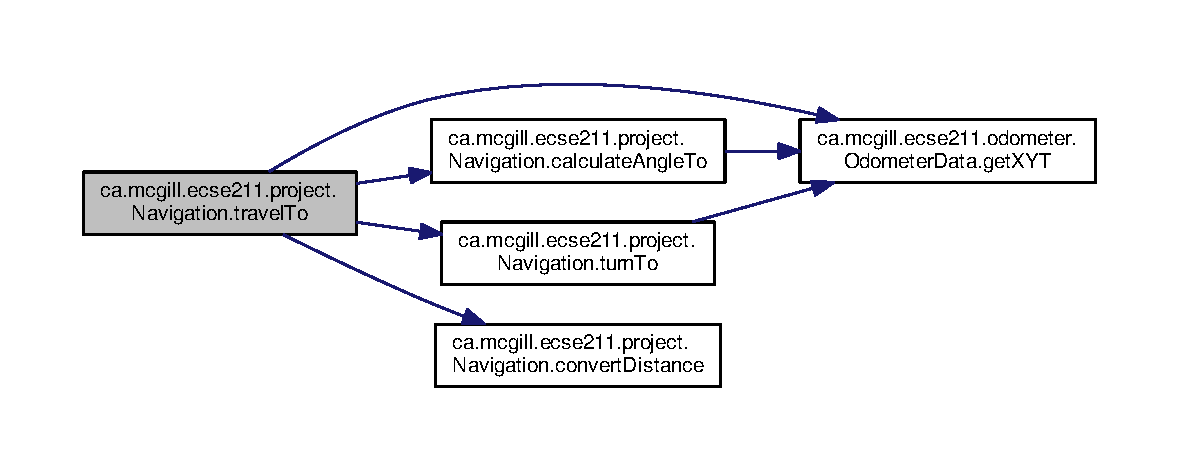
\includegraphics[width=350pt]{classca_1_1mcgill_1_1ecse211_1_1project_1_1_navigation_a3d8354490a2d8c36090d794c25d33421_cgraph}
\end{center}
\end{figure}
Here is the caller graph for this function\+:\nopagebreak
\begin{figure}[H]
\begin{center}
\leavevmode
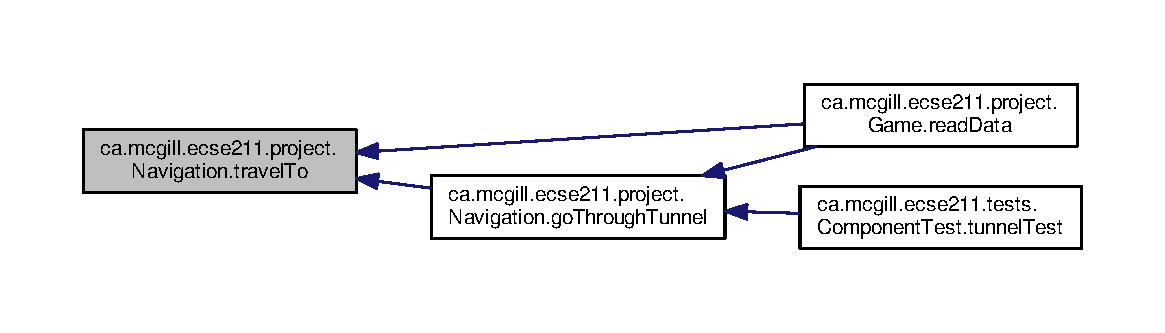
\includegraphics[width=350pt]{classca_1_1mcgill_1_1ecse211_1_1project_1_1_navigation_a3d8354490a2d8c36090d794c25d33421_icgraph}
\end{center}
\end{figure}
\mbox{\Hypertarget{classca_1_1mcgill_1_1ecse211_1_1project_1_1_navigation_ae7230e905494002087416294f12cae6a}\label{classca_1_1mcgill_1_1ecse211_1_1project_1_1_navigation_ae7230e905494002087416294f12cae6a}} 
\index{ca\+::mcgill\+::ecse211\+::project\+::\+Navigation@{ca\+::mcgill\+::ecse211\+::project\+::\+Navigation}!travel\+To\+With\+Correction@{travel\+To\+With\+Correction}}
\index{travel\+To\+With\+Correction@{travel\+To\+With\+Correction}!ca\+::mcgill\+::ecse211\+::project\+::\+Navigation@{ca\+::mcgill\+::ecse211\+::project\+::\+Navigation}}
\subsubsection{\texorpdfstring{travel\+To\+With\+Correction()}{travelToWithCorrection()}}
{\footnotesize\ttfamily void ca.\+mcgill.\+ecse211.\+project.\+Navigation.\+travel\+To\+With\+Correction (\begin{DoxyParamCaption}\item[{int}]{x,  }\item[{int}]{y,  }\item[{boolean}]{avoid }\end{DoxyParamCaption})}

This method makes the robot travel to a desired position by checking its orientation and corrects it if necessary to align with the lines on the grid.


\begin{DoxyParams}{Parameters}
{\em x} & The x coordinate to travel to \\
\hline
{\em y} & The y coordinate to travel to \\
\hline
{\em avoid} & This boolean decides if the robot will pay attention to readings from the ultrasonic sensor to avoid obstacles when navigating \\
\hline
\end{DoxyParams}


Definition at line 139 of file Navigation.\+java.


\begin{DoxyCode}
139                                                                   \{
140     \textcolor{keywordtype}{int} px = (int) Math.round(odometer.\hyperlink{classca_1_1mcgill_1_1ecse211_1_1odometer_1_1_odometer_data_a8f40f0264c68f0cbed4fff1723ae7863}{getXYT}()[0]);
141     \textcolor{keywordtype}{int} py = (int) Math.round(odometer.\hyperlink{classca_1_1mcgill_1_1ecse211_1_1odometer_1_1_odometer_data_a8f40f0264c68f0cbed4fff1723ae7863}{getXYT}()[1]);
142     \textcolor{keywordtype}{int}[] cur = \{px, py\};
143     \textcolor{keywordtype}{int}[] destination = \{x, y\};
144     ArrayList<Character> instruction = \textcolor{keyword}{new} ArrayList<Character>();
145 
146     \textcolor{comment}{// use path finder to find path based on the different areas the robot is in}
147     \textcolor{comment}{// OUT: instruction: contains a list of instruction for the robot to move to the destination}
148     \textcolor{keywordflow}{if} (GameParameters.getType(px, py) == GameParameters.AreaType.InStarting) \{
149       GameUtil.startingFinder.tryFindPath(cur, destination, instruction);
150     \} \textcolor{keywordflow}{else} \{
151       GameUtil.searchingFinder.tryFindPath(cur, destination, instruction);
152     \}
153 
154     \textcolor{comment}{// use the instruction modified by the pathFind to move to the destination}
155     \textcolor{keywordtype}{char} lastStep = \textcolor{charliteral}{' '};
156     \textcolor{keywordtype}{int} theta = 0;
157 
158     \textcolor{keywordflow}{while} (instruction.size() > 0) \{
159       \textcolor{keywordtype}{char} step = instruction.remove(instruction.size() - 1);
160       \textcolor{comment}{// if the step is different from the last one, rotate to corresponding rotation}
161       \textcolor{keywordflow}{if} (step != lastStep) \{
162         theta = charToRotation(step);
163         \hyperlink{classca_1_1mcgill_1_1ecse211_1_1project_1_1_navigation_a3bbe0645f2b3b3d0986b4a707fb5a00c}{turnTo}(theta);
164       \}
165 
166       \textcolor{comment}{// add a value to the robot traveled distance}
167       \textcolor{keywordflow}{if} (step == GameUtil.leftInstruction) \{
168         px--;
169       \} \textcolor{keywordflow}{else} \textcolor{keywordflow}{if} (step == GameUtil.rightInstruction) \{
170         px++;
171       \} \textcolor{keywordflow}{else} \textcolor{keywordflow}{if} (step == GameUtil.upInstruction) \{
172         py++;
173       \} \textcolor{keywordflow}{else} \{
174         py--;
175       \}
176       lastStep = step;
177 
178       \hyperlink{classca_1_1mcgill_1_1ecse211_1_1project_1_1_navigation_a48eeb9ae2da23664421e8da5642054c7}{moveWithCorrection}(1, theta);
179       \textcolor{comment}{// get the position of the robot}
180       \textcolor{keywordtype}{double}[] position = odometer.\hyperlink{classca_1_1mcgill_1_1ecse211_1_1odometer_1_1_odometer_data_a8f40f0264c68f0cbed4fff1723ae7863}{getXYT}();
181       \textcolor{keywordflow}{if} (Math.round(position[0]) == px && Math.round(position[1]) == py) \{
182         \textcolor{comment}{// this means that the robot is at the point, so set the position to the point}
183         odometer.\hyperlink{classca_1_1mcgill_1_1ecse211_1_1odometer_1_1_odometer_data_a2911d7215e47f3064defe016b46bfeef}{setX}(px);
184         odometer.\hyperlink{classca_1_1mcgill_1_1ecse211_1_1odometer_1_1_odometer_data_a82986438cd462e66520bc62bb4bd2b75}{setY}(py);
185       \} \textcolor{keywordflow}{else} \{
186         \textcolor{comment}{// otherwise some problem might happened and we are not at the desired point, push the}
187         \textcolor{comment}{// instruction back}
188         instruction.add(step);
189         \textcolor{comment}{// reset the added value to last point}
190         \textcolor{keywordflow}{if} (step == GameUtil.leftInstruction) \{
191           px++;
192         \} \textcolor{keywordflow}{else} \textcolor{keywordflow}{if} (step == GameUtil.rightInstruction) \{
193           px--;
194         \} \textcolor{keywordflow}{else} \textcolor{keywordflow}{if} (step == GameUtil.upInstruction) \{
195           py--;
196         \} \textcolor{keywordflow}{else} \{
197           py++;
198         \}
199       \}
200     \}
201   \}
\end{DoxyCode}
Here is the call graph for this function\+:\nopagebreak
\begin{figure}[H]
\begin{center}
\leavevmode
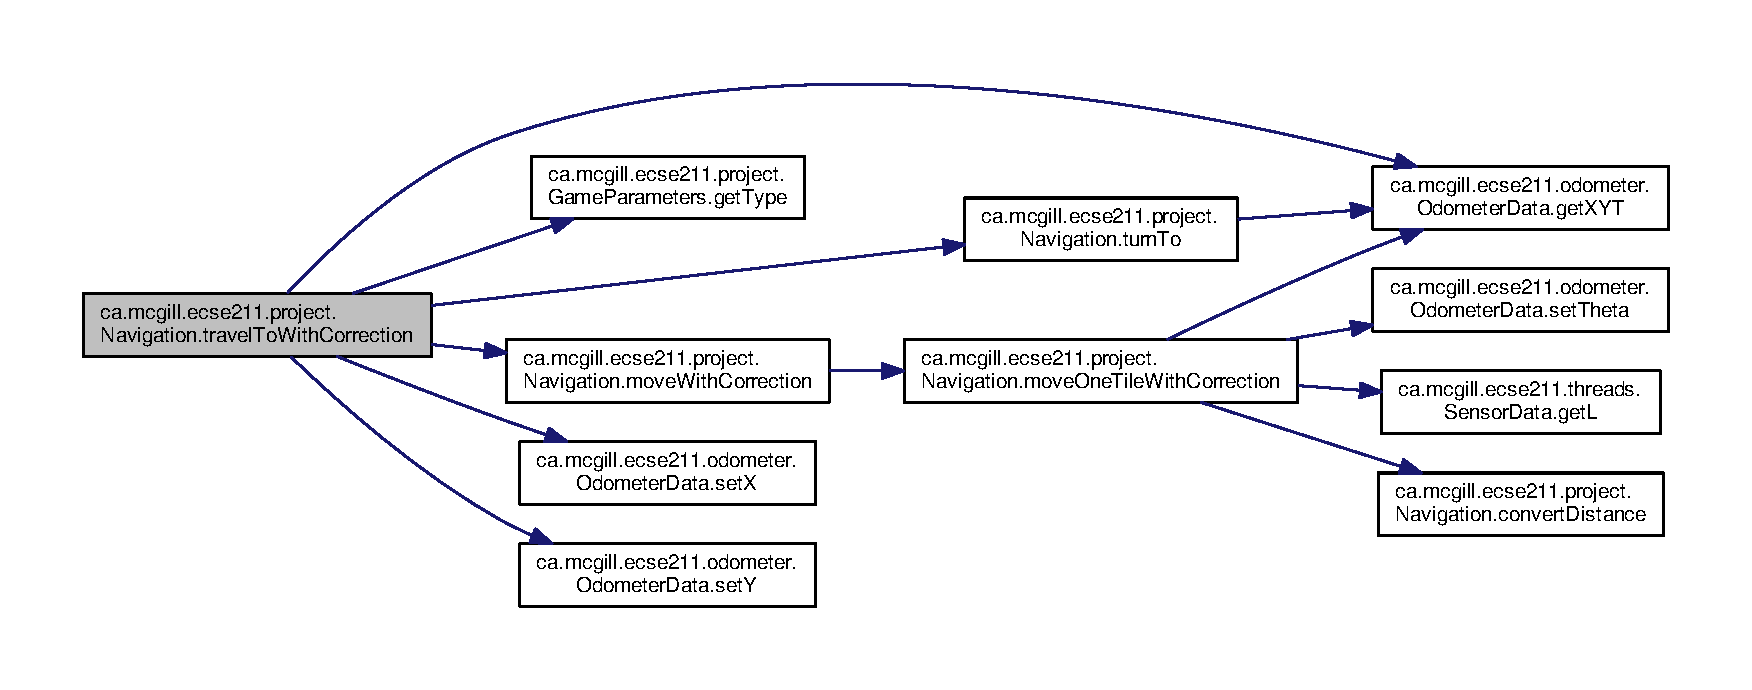
\includegraphics[width=350pt]{classca_1_1mcgill_1_1ecse211_1_1project_1_1_navigation_ae7230e905494002087416294f12cae6a_cgraph}
\end{center}
\end{figure}
Here is the caller graph for this function\+:\nopagebreak
\begin{figure}[H]
\begin{center}
\leavevmode
\includegraphics[width=350pt]{classca_1_1mcgill_1_1ecse211_1_1project_1_1_navigation_ae7230e905494002087416294f12cae6a_icgraph}
\end{center}
\end{figure}
\mbox{\Hypertarget{classca_1_1mcgill_1_1ecse211_1_1project_1_1_navigation_ad74286ad36d333bfaf57661837457b76}\label{classca_1_1mcgill_1_1ecse211_1_1project_1_1_navigation_ad74286ad36d333bfaf57661837457b76}} 
\index{ca\+::mcgill\+::ecse211\+::project\+::\+Navigation@{ca\+::mcgill\+::ecse211\+::project\+::\+Navigation}!turn@{turn}}
\index{turn@{turn}!ca\+::mcgill\+::ecse211\+::project\+::\+Navigation@{ca\+::mcgill\+::ecse211\+::project\+::\+Navigation}}
\subsubsection{\texorpdfstring{turn()}{turn()}}
{\footnotesize\ttfamily void ca.\+mcgill.\+ecse211.\+project.\+Navigation.\+turn (\begin{DoxyParamCaption}\item[{int}]{angle }\end{DoxyParamCaption})}

This method rotates the robot by a certain angle


\begin{DoxyParams}{Parameters}
{\em angle} & The angle (in degrees) to rotate our robot to \\
\hline
\end{DoxyParams}


Definition at line 614 of file Navigation.\+java.


\begin{DoxyCode}
614                               \{
615     leftMotor.rotate(convertAngle(Game.WHEEL\_RAD, Game.TRACK, angle), \textcolor{keyword}{true});
616     rightMotor.rotate(-convertAngle(Game.WHEEL\_RAD, Game.TRACK, angle), \textcolor{keyword}{false});
617   \}
\end{DoxyCode}
Here is the caller graph for this function\+:\nopagebreak
\begin{figure}[H]
\begin{center}
\leavevmode
\includegraphics[width=350pt]{classca_1_1mcgill_1_1ecse211_1_1project_1_1_navigation_ad74286ad36d333bfaf57661837457b76_icgraph}
\end{center}
\end{figure}
\mbox{\Hypertarget{classca_1_1mcgill_1_1ecse211_1_1project_1_1_navigation_a3bbe0645f2b3b3d0986b4a707fb5a00c}\label{classca_1_1mcgill_1_1ecse211_1_1project_1_1_navigation_a3bbe0645f2b3b3d0986b4a707fb5a00c}} 
\index{ca\+::mcgill\+::ecse211\+::project\+::\+Navigation@{ca\+::mcgill\+::ecse211\+::project\+::\+Navigation}!turn\+To@{turn\+To}}
\index{turn\+To@{turn\+To}!ca\+::mcgill\+::ecse211\+::project\+::\+Navigation@{ca\+::mcgill\+::ecse211\+::project\+::\+Navigation}}
\subsubsection{\texorpdfstring{turn\+To()}{turnTo()}}
{\footnotesize\ttfamily synchronized void ca.\+mcgill.\+ecse211.\+project.\+Navigation.\+turn\+To (\begin{DoxyParamCaption}\item[{double}]{angle }\end{DoxyParamCaption})}

This method turns our robot to a desired angle


\begin{DoxyParams}{Parameters}
{\em angle} & The angle we want our robot to turn to (in degrees) \\
\hline
\end{DoxyParams}


Definition at line 353 of file Navigation.\+java.


\begin{DoxyCode}
353                                                 \{
354     \textcolor{keywordtype}{double} dTheta;
355 
356     dTheta = angle - odometer.\hyperlink{classca_1_1mcgill_1_1ecse211_1_1odometer_1_1_odometer_data_a8f40f0264c68f0cbed4fff1723ae7863}{getXYT}()[2];
357     \textcolor{keywordflow}{if} (dTheta < 0)
358       dTheta += 360;
359 
360     \textcolor{comment}{// TURN RIGHT}
361     \textcolor{keywordflow}{if} (dTheta > 180) \{
362       leftMotor.setSpeed(ROTATE\_SPEED);
363       rightMotor.setSpeed(ROTATE\_SPEED);
364       \textcolor{keywordflow}{try} \{
365         Thread.sleep(100);
366       \} \textcolor{keywordflow}{catch} (InterruptedException e) \{
367         e.printStackTrace();
368       \}
369       leftMotor.rotate(-convertAngle(Game.WHEEL\_RAD, Game.TRACK, 360 - dTheta), \textcolor{keyword}{true});
370       rightMotor.rotate(convertAngle(Game.WHEEL\_RAD, Game.TRACK, 360 - dTheta), \textcolor{keyword}{false});
371     \}
372     \textcolor{comment}{// TURN LEFT}
373     \textcolor{keywordflow}{else} \{
374       leftMotor.setSpeed(ROTATE\_SPEED);
375       rightMotor.setSpeed(ROTATE\_SPEED);
376       \textcolor{keywordflow}{try} \{
377         Thread.sleep(100);
378       \} \textcolor{keywordflow}{catch} (InterruptedException e) \{
379         e.printStackTrace();
380       \}
381       leftMotor.rotate(convertAngle(Game.WHEEL\_RAD, Game.TRACK, dTheta), \textcolor{keyword}{true});
382       rightMotor.rotate(-convertAngle(Game.WHEEL\_RAD, Game.TRACK, dTheta), \textcolor{keyword}{false});
383     \}
384   \}
\end{DoxyCode}
Here is the call graph for this function\+:\nopagebreak
\begin{figure}[H]
\begin{center}
\leavevmode
\includegraphics[width=350pt]{classca_1_1mcgill_1_1ecse211_1_1project_1_1_navigation_a3bbe0645f2b3b3d0986b4a707fb5a00c_cgraph}
\end{center}
\end{figure}
Here is the caller graph for this function\+:\nopagebreak
\begin{figure}[H]
\begin{center}
\leavevmode
\includegraphics[width=350pt]{classca_1_1mcgill_1_1ecse211_1_1project_1_1_navigation_a3bbe0645f2b3b3d0986b4a707fb5a00c_icgraph}
\end{center}
\end{figure}


The documentation for this class was generated from the following file\+:\begin{DoxyCompactItemize}
\item 
/home/ccc/\+Final\+Project/src/ca/mcgill/ecse211/project/\hyperlink{_navigation_8java}{Navigation.\+java}\end{DoxyCompactItemize}

\hypertarget{classca_1_1mcgill_1_1ecse211_1_1odometer_1_1_odometer}{}\section{ca.\+mcgill.\+ecse211.\+odometer.\+Odometer Class Reference}
\label{classca_1_1mcgill_1_1ecse211_1_1odometer_1_1_odometer}\index{ca.\+mcgill.\+ecse211.\+odometer.\+Odometer@{ca.\+mcgill.\+ecse211.\+odometer.\+Odometer}}


Inheritance diagram for ca.\+mcgill.\+ecse211.\+odometer.\+Odometer\+:\nopagebreak
\begin{figure}[H]
\begin{center}
\leavevmode
\includegraphics[width=298pt]{classca_1_1mcgill_1_1ecse211_1_1odometer_1_1_odometer__inherit__graph}
\end{center}
\end{figure}


Collaboration diagram for ca.\+mcgill.\+ecse211.\+odometer.\+Odometer\+:\nopagebreak
\begin{figure}[H]
\begin{center}
\leavevmode
\includegraphics[width=298pt]{classca_1_1mcgill_1_1ecse211_1_1odometer_1_1_odometer__coll__graph}
\end{center}
\end{figure}
\subsection*{Public Member Functions}
\begin{DoxyCompactItemize}
\item 
void \hyperlink{classca_1_1mcgill_1_1ecse211_1_1odometer_1_1_odometer_af0ff4c5121973a8310cf986e25fa0d87}{run} ()
\end{DoxyCompactItemize}
\subsection*{Static Public Member Functions}
\begin{DoxyCompactItemize}
\item 
static synchronized \hyperlink{classca_1_1mcgill_1_1ecse211_1_1odometer_1_1_odometer}{Odometer} \hyperlink{classca_1_1mcgill_1_1ecse211_1_1odometer_1_1_odometer_a99171f11e34dea918fa9dd069d721439}{get\+Odometer} (E\+V3\+Large\+Regulated\+Motor left\+Motor, E\+V3\+Large\+Regulated\+Motor right\+Motor, final double T\+R\+A\+CK, final double W\+H\+E\+E\+L\+\_\+\+R\+AD)  throws Odometer\+Exceptions 
\item 
static synchronized \hyperlink{classca_1_1mcgill_1_1ecse211_1_1odometer_1_1_odometer}{Odometer} \hyperlink{classca_1_1mcgill_1_1ecse211_1_1odometer_1_1_odometer_a4e069b5a96cd43b29af0785244a99b51}{get\+Odometer} ()  throws Odometer\+Exceptions 
\end{DoxyCompactItemize}
\subsection*{Additional Inherited Members}


\subsection{Detailed Description}
This class implements odometry on our robot.

\begin{DoxyAuthor}{Author}
Caspar Cedro 

Percy Chen 

Patrick Erath 

Anssam Ghezala 

Susan Matuszewski 

Kamy Moussavi Kafi 
\end{DoxyAuthor}


Definition at line 16 of file Odometer.\+java.



\subsection{Member Function Documentation}
\mbox{\Hypertarget{classca_1_1mcgill_1_1ecse211_1_1odometer_1_1_odometer_a99171f11e34dea918fa9dd069d721439}\label{classca_1_1mcgill_1_1ecse211_1_1odometer_1_1_odometer_a99171f11e34dea918fa9dd069d721439}} 
\index{ca\+::mcgill\+::ecse211\+::odometer\+::\+Odometer@{ca\+::mcgill\+::ecse211\+::odometer\+::\+Odometer}!get\+Odometer@{get\+Odometer}}
\index{get\+Odometer@{get\+Odometer}!ca\+::mcgill\+::ecse211\+::odometer\+::\+Odometer@{ca\+::mcgill\+::ecse211\+::odometer\+::\+Odometer}}
\subsubsection{\texorpdfstring{get\+Odometer()}{getOdometer()}\hspace{0.1cm}{\footnotesize\ttfamily [1/2]}}
{\footnotesize\ttfamily static synchronized \hyperlink{classca_1_1mcgill_1_1ecse211_1_1odometer_1_1_odometer}{Odometer} ca.\+mcgill.\+ecse211.\+odometer.\+Odometer.\+get\+Odometer (\begin{DoxyParamCaption}\item[{E\+V3\+Large\+Regulated\+Motor}]{left\+Motor,  }\item[{E\+V3\+Large\+Regulated\+Motor}]{right\+Motor,  }\item[{final double}]{T\+R\+A\+CK,  }\item[{final double}]{W\+H\+E\+E\+L\+\_\+\+R\+AD }\end{DoxyParamCaption}) throws \hyperlink{classca_1_1mcgill_1_1ecse211_1_1odometer_1_1_odometer_exceptions}{Odometer\+Exceptions}\hspace{0.3cm}{\ttfamily [static]}}

This method is meant to ensure only one instance of the odometer is used throughout the code.


\begin{DoxyParams}{Parameters}
{\em left\+Motor} & The E\+V3\+Large\+Regulated\+Motor instance for our left motor \\
\hline
{\em right\+Motor} & The E\+V3\+Large\+Regulated\+Motor instance for our right motor \\
\hline
\end{DoxyParams}
\begin{DoxyReturn}{Returns}
new or existing \hyperlink{classca_1_1mcgill_1_1ecse211_1_1odometer_1_1_odometer}{Odometer} Object 
\end{DoxyReturn}

\begin{DoxyExceptions}{Exceptions}
{\em \hyperlink{classca_1_1mcgill_1_1ecse211_1_1odometer_1_1_odometer_exceptions}{Odometer\+Exceptions}} & \\
\hline
\end{DoxyExceptions}


Definition at line 69 of file Odometer.\+java.


\begin{DoxyCode}
71                                 \{
72     \textcolor{keywordflow}{if} (odometer != null) \{ \textcolor{comment}{// Return existing object}
73       \textcolor{keywordflow}{return} odometer;
74     \} \textcolor{keywordflow}{else} \{ \textcolor{comment}{// create object and return it}
75       odometer = \textcolor{keyword}{new} Odometer(leftMotor, rightMotor, TRACK, WHEEL\_RAD);
76       \textcolor{keywordflow}{return} odometer;
77     \}
78   \}
\end{DoxyCode}
Here is the caller graph for this function\+:\nopagebreak
\begin{figure}[H]
\begin{center}
\leavevmode
\includegraphics[width=350pt]{classca_1_1mcgill_1_1ecse211_1_1odometer_1_1_odometer_a99171f11e34dea918fa9dd069d721439_icgraph}
\end{center}
\end{figure}
\mbox{\Hypertarget{classca_1_1mcgill_1_1ecse211_1_1odometer_1_1_odometer_a4e069b5a96cd43b29af0785244a99b51}\label{classca_1_1mcgill_1_1ecse211_1_1odometer_1_1_odometer_a4e069b5a96cd43b29af0785244a99b51}} 
\index{ca\+::mcgill\+::ecse211\+::odometer\+::\+Odometer@{ca\+::mcgill\+::ecse211\+::odometer\+::\+Odometer}!get\+Odometer@{get\+Odometer}}
\index{get\+Odometer@{get\+Odometer}!ca\+::mcgill\+::ecse211\+::odometer\+::\+Odometer@{ca\+::mcgill\+::ecse211\+::odometer\+::\+Odometer}}
\subsubsection{\texorpdfstring{get\+Odometer()}{getOdometer()}\hspace{0.1cm}{\footnotesize\ttfamily [2/2]}}
{\footnotesize\ttfamily static synchronized \hyperlink{classca_1_1mcgill_1_1ecse211_1_1odometer_1_1_odometer}{Odometer} ca.\+mcgill.\+ecse211.\+odometer.\+Odometer.\+get\+Odometer (\begin{DoxyParamCaption}{ }\end{DoxyParamCaption}) throws \hyperlink{classca_1_1mcgill_1_1ecse211_1_1odometer_1_1_odometer_exceptions}{Odometer\+Exceptions}\hspace{0.3cm}{\ttfamily [static]}}

This class is meant to return the existing \hyperlink{classca_1_1mcgill_1_1ecse211_1_1odometer_1_1_odometer}{Odometer} Object. It is meant to be used only if an odometer object has been created

\begin{DoxyReturn}{Returns}
error if no previous odometer exists 
\end{DoxyReturn}


Definition at line 86 of file Odometer.\+java.


\begin{DoxyCode}
86                                                                               \{
87 
88     \textcolor{keywordflow}{if} (odometer == null) \{
89       \textcolor{keywordflow}{throw} \textcolor{keyword}{new} OdometerExceptions(\textcolor{stringliteral}{"No previous Odometer exits."});
90 
91     \}
92     \textcolor{keywordflow}{return} odometer;
93   \}
\end{DoxyCode}
\mbox{\Hypertarget{classca_1_1mcgill_1_1ecse211_1_1odometer_1_1_odometer_af0ff4c5121973a8310cf986e25fa0d87}\label{classca_1_1mcgill_1_1ecse211_1_1odometer_1_1_odometer_af0ff4c5121973a8310cf986e25fa0d87}} 
\index{ca\+::mcgill\+::ecse211\+::odometer\+::\+Odometer@{ca\+::mcgill\+::ecse211\+::odometer\+::\+Odometer}!run@{run}}
\index{run@{run}!ca\+::mcgill\+::ecse211\+::odometer\+::\+Odometer@{ca\+::mcgill\+::ecse211\+::odometer\+::\+Odometer}}
\subsubsection{\texorpdfstring{run()}{run()}}
{\footnotesize\ttfamily void ca.\+mcgill.\+ecse211.\+odometer.\+Odometer.\+run (\begin{DoxyParamCaption}{ }\end{DoxyParamCaption})}

This method is called when our \hyperlink{classca_1_1mcgill_1_1ecse211_1_1odometer_1_1_odometer}{Odometer} object is started as a thread and begins to keep track of motor rotations 

Definition at line 99 of file Odometer.\+java.


\begin{DoxyCode}
99                     \{
100     \textcolor{keywordtype}{long} updateStart, updateEnd;
101 
102     \textcolor{keywordflow}{while} (\textcolor{keyword}{true}) \{
103       updateStart = System.currentTimeMillis();
104 
105       \textcolor{comment}{// TODO Calculate new robot position based on tachometer counts}
106       \textcolor{keywordtype}{double} distL, distR, deltaD, deltaT, dX, dY;
107       \textcolor{keywordtype}{int} nowTachoL, nowTachoR;
108       position = odometer.\hyperlink{classca_1_1mcgill_1_1ecse211_1_1odometer_1_1_odometer_data_a8f40f0264c68f0cbed4fff1723ae7863}{getXYT}();
109 
110       \textcolor{comment}{// Calculate the change in distances and Theta with motor tacho counts}
111       nowTachoL = leftMotor.getTachoCount();
112       nowTachoR = rightMotor.getTachoCount();
113       distL = 3.14159 * WHEEL\_RAD * (nowTachoL - leftMotorTachoCount) / 180;
114       distR = 3.14159 * WHEEL\_RAD * (nowTachoR - rightMotorTachoCount) / 180;
115       leftMotorTachoCount = nowTachoL;
116       rightMotorTachoCount = nowTachoR;
117       deltaD = 0.5 * (distL + distR);
118       deltaT = (distL - distR) / TRACK;
119 
120       \textcolor{keywordtype}{double} Theta = Math.toRadians(position[2]);
121       Theta += deltaT;
122       dX = deltaD * Math.sin(Theta);
123       dY = deltaD * Math.cos(Theta);
124 
125 
126       \textcolor{comment}{// TODO Update odometer values with new calculated values}
127       odometer.\hyperlink{classca_1_1mcgill_1_1ecse211_1_1odometer_1_1_odometer_data_aaa06f190d634299fcb1b97a1891dad85}{update}(dX / Game.TILE, dY / Game.TILE, Math.toDegrees(deltaT));
128 
129 
130       \textcolor{comment}{// this ensures that the odometer only runs once every period}
131       updateEnd = System.currentTimeMillis();
132       \textcolor{keywordflow}{if} (updateEnd - updateStart < ODOMETER\_PERIOD) \{
133         \textcolor{keywordflow}{try} \{
134           Thread.sleep(ODOMETER\_PERIOD - (updateEnd - updateStart));
135         \} \textcolor{keywordflow}{catch} (InterruptedException e) \{
136           \textcolor{comment}{// there is nothing to be done}
137         \}
138       \}
139     \}
140   \}
\end{DoxyCode}
Here is the call graph for this function\+:\nopagebreak
\begin{figure}[H]
\begin{center}
\leavevmode
\includegraphics[width=350pt]{classca_1_1mcgill_1_1ecse211_1_1odometer_1_1_odometer_af0ff4c5121973a8310cf986e25fa0d87_cgraph}
\end{center}
\end{figure}


The documentation for this class was generated from the following file\+:\begin{DoxyCompactItemize}
\item 
/home/ccc/\+Final\+Project/src/ca/mcgill/ecse211/odometer/\hyperlink{_odometer_8java}{Odometer.\+java}\end{DoxyCompactItemize}

\hypertarget{classca_1_1mcgill_1_1ecse211_1_1odometer_1_1_odometer_data}{}\section{ca.\+mcgill.\+ecse211.\+odometer.\+Odometer\+Data Class Reference}
\label{classca_1_1mcgill_1_1ecse211_1_1odometer_1_1_odometer_data}\index{ca.\+mcgill.\+ecse211.\+odometer.\+Odometer\+Data@{ca.\+mcgill.\+ecse211.\+odometer.\+Odometer\+Data}}


Inheritance diagram for ca.\+mcgill.\+ecse211.\+odometer.\+Odometer\+Data\+:
\nopagebreak
\begin{figure}[H]
\begin{center}
\leavevmode
\includegraphics[width=222pt]{classca_1_1mcgill_1_1ecse211_1_1odometer_1_1_odometer_data__inherit__graph}
\end{center}
\end{figure}
\subsection*{Public Member Functions}
\begin{DoxyCompactItemize}
\item 
double \mbox{[}$\,$\mbox{]} \hyperlink{classca_1_1mcgill_1_1ecse211_1_1odometer_1_1_odometer_data_a8f40f0264c68f0cbed4fff1723ae7863}{get\+X\+YT} ()
\item 
void \hyperlink{classca_1_1mcgill_1_1ecse211_1_1odometer_1_1_odometer_data_aaa06f190d634299fcb1b97a1891dad85}{update} (double dx, double dy, double dtheta)
\item 
void \hyperlink{classca_1_1mcgill_1_1ecse211_1_1odometer_1_1_odometer_data_a2ebc18a13aea6276122d9ef4ee100bb9}{set\+X\+YT} (double x, double y, double theta)
\item 
void \hyperlink{classca_1_1mcgill_1_1ecse211_1_1odometer_1_1_odometer_data_a2911d7215e47f3064defe016b46bfeef}{setX} (double x)
\item 
void \hyperlink{classca_1_1mcgill_1_1ecse211_1_1odometer_1_1_odometer_data_a82986438cd462e66520bc62bb4bd2b75}{setY} (double y)
\item 
void \hyperlink{classca_1_1mcgill_1_1ecse211_1_1odometer_1_1_odometer_data_a419b8f07c2c5374411c8e62298e9a402}{set\+Theta} (double theta)
\end{DoxyCompactItemize}
\subsection*{Static Public Member Functions}
\begin{DoxyCompactItemize}
\item 
static synchronized \hyperlink{classca_1_1mcgill_1_1ecse211_1_1odometer_1_1_odometer_data}{Odometer\+Data} \hyperlink{classca_1_1mcgill_1_1ecse211_1_1odometer_1_1_odometer_data_afff2d760dd1f861b580f3eacef37f1cc}{get\+Odometer\+Data} ()  throws Odometer\+Exceptions 
\end{DoxyCompactItemize}
\subsection*{Protected Member Functions}
\begin{DoxyCompactItemize}
\item 
\hyperlink{classca_1_1mcgill_1_1ecse211_1_1odometer_1_1_odometer_data_a91412854b75c41bf3af7c8892ec0fe87}{Odometer\+Data} ()
\end{DoxyCompactItemize}


\subsection{Detailed Description}
This class stores and provides thread safe access to the odometer data.

\begin{DoxyAuthor}{Author}
Rodrigo Silva 

Dirk Dubois 

Derek Yu 

Karim El-\/\+Baba 

Michael Smith 
\end{DoxyAuthor}


Definition at line 16 of file Odometer\+Data.\+java.



\subsection{Constructor \& Destructor Documentation}
\mbox{\Hypertarget{classca_1_1mcgill_1_1ecse211_1_1odometer_1_1_odometer_data_a91412854b75c41bf3af7c8892ec0fe87}\label{classca_1_1mcgill_1_1ecse211_1_1odometer_1_1_odometer_data_a91412854b75c41bf3af7c8892ec0fe87}} 
\index{ca\+::mcgill\+::ecse211\+::odometer\+::\+Odometer\+Data@{ca\+::mcgill\+::ecse211\+::odometer\+::\+Odometer\+Data}!Odometer\+Data@{Odometer\+Data}}
\index{Odometer\+Data@{Odometer\+Data}!ca\+::mcgill\+::ecse211\+::odometer\+::\+Odometer\+Data@{ca\+::mcgill\+::ecse211\+::odometer\+::\+Odometer\+Data}}
\subsubsection{\texorpdfstring{Odometer\+Data()}{OdometerData()}}
{\footnotesize\ttfamily ca.\+mcgill.\+ecse211.\+odometer.\+Odometer\+Data.\+Odometer\+Data (\begin{DoxyParamCaption}{ }\end{DoxyParamCaption})\hspace{0.3cm}{\ttfamily [protected]}}

Default constructor. The constructor is private. A factory is used instead such that only one instance of this class is ever created. 

Definition at line 47 of file Odometer\+Data.\+java.

Here is the caller graph for this function\+:
\nopagebreak
\begin{figure}[H]
\begin{center}
\leavevmode
\includegraphics[width=350pt]{classca_1_1mcgill_1_1ecse211_1_1odometer_1_1_odometer_data_a91412854b75c41bf3af7c8892ec0fe87_icgraph}
\end{center}
\end{figure}


\subsection{Member Function Documentation}
\mbox{\Hypertarget{classca_1_1mcgill_1_1ecse211_1_1odometer_1_1_odometer_data_afff2d760dd1f861b580f3eacef37f1cc}\label{classca_1_1mcgill_1_1ecse211_1_1odometer_1_1_odometer_data_afff2d760dd1f861b580f3eacef37f1cc}} 
\index{ca\+::mcgill\+::ecse211\+::odometer\+::\+Odometer\+Data@{ca\+::mcgill\+::ecse211\+::odometer\+::\+Odometer\+Data}!get\+Odometer\+Data@{get\+Odometer\+Data}}
\index{get\+Odometer\+Data@{get\+Odometer\+Data}!ca\+::mcgill\+::ecse211\+::odometer\+::\+Odometer\+Data@{ca\+::mcgill\+::ecse211\+::odometer\+::\+Odometer\+Data}}
\subsubsection{\texorpdfstring{get\+Odometer\+Data()}{getOdometerData()}}
{\footnotesize\ttfamily static synchronized \hyperlink{classca_1_1mcgill_1_1ecse211_1_1odometer_1_1_odometer_data}{Odometer\+Data} ca.\+mcgill.\+ecse211.\+odometer.\+Odometer\+Data.\+get\+Odometer\+Data (\begin{DoxyParamCaption}{ }\end{DoxyParamCaption}) throws \hyperlink{classca_1_1mcgill_1_1ecse211_1_1odometer_1_1_odometer_exceptions}{Odometer\+Exceptions}\hspace{0.3cm}{\ttfamily [static]}}

\hyperlink{classca_1_1mcgill_1_1ecse211_1_1odometer_1_1_odometer_data}{Odometer\+Data} factory. Returns an \hyperlink{classca_1_1mcgill_1_1ecse211_1_1odometer_1_1_odometer_data}{Odometer\+Data} instance and makes sure that only one instance is ever created. If the user tries to instantiate multiple objects, the method throws a Multiple\+Odometer\+Data\+Exception.

\begin{DoxyReturn}{Returns}
An \hyperlink{classca_1_1mcgill_1_1ecse211_1_1odometer_1_1_odometer_data}{Odometer\+Data} object 
\end{DoxyReturn}

\begin{DoxyExceptions}{Exceptions}
{\em \hyperlink{classca_1_1mcgill_1_1ecse211_1_1odometer_1_1_odometer_exceptions}{Odometer\+Exceptions}} & \\
\hline
\end{DoxyExceptions}


Definition at line 61 of file Odometer\+Data.\+java.

Here is the call graph for this function\+:
\nopagebreak
\begin{figure}[H]
\begin{center}
\leavevmode
\includegraphics[width=350pt]{classca_1_1mcgill_1_1ecse211_1_1odometer_1_1_odometer_data_afff2d760dd1f861b580f3eacef37f1cc_cgraph}
\end{center}
\end{figure}
\mbox{\Hypertarget{classca_1_1mcgill_1_1ecse211_1_1odometer_1_1_odometer_data_a8f40f0264c68f0cbed4fff1723ae7863}\label{classca_1_1mcgill_1_1ecse211_1_1odometer_1_1_odometer_data_a8f40f0264c68f0cbed4fff1723ae7863}} 
\index{ca\+::mcgill\+::ecse211\+::odometer\+::\+Odometer\+Data@{ca\+::mcgill\+::ecse211\+::odometer\+::\+Odometer\+Data}!get\+X\+YT@{get\+X\+YT}}
\index{get\+X\+YT@{get\+X\+YT}!ca\+::mcgill\+::ecse211\+::odometer\+::\+Odometer\+Data@{ca\+::mcgill\+::ecse211\+::odometer\+::\+Odometer\+Data}}
\subsubsection{\texorpdfstring{get\+X\+Y\+T()}{getXYT()}}
{\footnotesize\ttfamily double \mbox{[}$\,$\mbox{]} ca.\+mcgill.\+ecse211.\+odometer.\+Odometer\+Data.\+get\+X\+YT (\begin{DoxyParamCaption}{ }\end{DoxyParamCaption})}

Return the Odomometer data. 

Writes the current position and orientation of the robot onto the odo\+Data array. odo\+Data\mbox{[}0\mbox{]} = x, odo\+Data\mbox{[}1\mbox{]} = y; odo\+Data\mbox{[}2\mbox{]} = theta;


\begin{DoxyParams}{Parameters}
{\em position} & the array to store the odometer data \\
\hline
\end{DoxyParams}
\begin{DoxyReturn}{Returns}
the odometer data. 
\end{DoxyReturn}


Definition at line 84 of file Odometer\+Data.\+java.

Here is the caller graph for this function\+:
\nopagebreak
\begin{figure}[H]
\begin{center}
\leavevmode
\includegraphics[width=350pt]{classca_1_1mcgill_1_1ecse211_1_1odometer_1_1_odometer_data_a8f40f0264c68f0cbed4fff1723ae7863_icgraph}
\end{center}
\end{figure}
\mbox{\Hypertarget{classca_1_1mcgill_1_1ecse211_1_1odometer_1_1_odometer_data_a419b8f07c2c5374411c8e62298e9a402}\label{classca_1_1mcgill_1_1ecse211_1_1odometer_1_1_odometer_data_a419b8f07c2c5374411c8e62298e9a402}} 
\index{ca\+::mcgill\+::ecse211\+::odometer\+::\+Odometer\+Data@{ca\+::mcgill\+::ecse211\+::odometer\+::\+Odometer\+Data}!set\+Theta@{set\+Theta}}
\index{set\+Theta@{set\+Theta}!ca\+::mcgill\+::ecse211\+::odometer\+::\+Odometer\+Data@{ca\+::mcgill\+::ecse211\+::odometer\+::\+Odometer\+Data}}
\subsubsection{\texorpdfstring{set\+Theta()}{setTheta()}}
{\footnotesize\ttfamily void ca.\+mcgill.\+ecse211.\+odometer.\+Odometer\+Data.\+set\+Theta (\begin{DoxyParamCaption}\item[{double}]{theta }\end{DoxyParamCaption})}

Overrides theta. Use for odometry correction.


\begin{DoxyParams}{Parameters}
{\em theta} & the value of theta \\
\hline
\end{DoxyParams}


Definition at line 197 of file Odometer\+Data.\+java.

Here is the caller graph for this function\+:
\nopagebreak
\begin{figure}[H]
\begin{center}
\leavevmode
\includegraphics[width=350pt]{classca_1_1mcgill_1_1ecse211_1_1odometer_1_1_odometer_data_a419b8f07c2c5374411c8e62298e9a402_icgraph}
\end{center}
\end{figure}
\mbox{\Hypertarget{classca_1_1mcgill_1_1ecse211_1_1odometer_1_1_odometer_data_a2911d7215e47f3064defe016b46bfeef}\label{classca_1_1mcgill_1_1ecse211_1_1odometer_1_1_odometer_data_a2911d7215e47f3064defe016b46bfeef}} 
\index{ca\+::mcgill\+::ecse211\+::odometer\+::\+Odometer\+Data@{ca\+::mcgill\+::ecse211\+::odometer\+::\+Odometer\+Data}!setX@{setX}}
\index{setX@{setX}!ca\+::mcgill\+::ecse211\+::odometer\+::\+Odometer\+Data@{ca\+::mcgill\+::ecse211\+::odometer\+::\+Odometer\+Data}}
\subsubsection{\texorpdfstring{set\+X()}{setX()}}
{\footnotesize\ttfamily void ca.\+mcgill.\+ecse211.\+odometer.\+Odometer\+Data.\+setX (\begin{DoxyParamCaption}\item[{double}]{x }\end{DoxyParamCaption})}

Overrides x. Use for odometry correction.


\begin{DoxyParams}{Parameters}
{\em x} & the value of x \\
\hline
\end{DoxyParams}


Definition at line 161 of file Odometer\+Data.\+java.

Here is the caller graph for this function\+:
\nopagebreak
\begin{figure}[H]
\begin{center}
\leavevmode
\includegraphics[width=350pt]{classca_1_1mcgill_1_1ecse211_1_1odometer_1_1_odometer_data_a2911d7215e47f3064defe016b46bfeef_icgraph}
\end{center}
\end{figure}
\mbox{\Hypertarget{classca_1_1mcgill_1_1ecse211_1_1odometer_1_1_odometer_data_a2ebc18a13aea6276122d9ef4ee100bb9}\label{classca_1_1mcgill_1_1ecse211_1_1odometer_1_1_odometer_data_a2ebc18a13aea6276122d9ef4ee100bb9}} 
\index{ca\+::mcgill\+::ecse211\+::odometer\+::\+Odometer\+Data@{ca\+::mcgill\+::ecse211\+::odometer\+::\+Odometer\+Data}!set\+X\+YT@{set\+X\+YT}}
\index{set\+X\+YT@{set\+X\+YT}!ca\+::mcgill\+::ecse211\+::odometer\+::\+Odometer\+Data@{ca\+::mcgill\+::ecse211\+::odometer\+::\+Odometer\+Data}}
\subsubsection{\texorpdfstring{set\+X\+Y\+T()}{setXYT()}}
{\footnotesize\ttfamily void ca.\+mcgill.\+ecse211.\+odometer.\+Odometer\+Data.\+set\+X\+YT (\begin{DoxyParamCaption}\item[{double}]{x,  }\item[{double}]{y,  }\item[{double}]{theta }\end{DoxyParamCaption})}

Overrides the values of x, y and theta. Use for odometry correction.


\begin{DoxyParams}{Parameters}
{\em x} & the value of x \\
\hline
{\em y} & the value of y \\
\hline
{\em theta} & the value of theta \\
\hline
\end{DoxyParams}


Definition at line 141 of file Odometer\+Data.\+java.

\mbox{\Hypertarget{classca_1_1mcgill_1_1ecse211_1_1odometer_1_1_odometer_data_a82986438cd462e66520bc62bb4bd2b75}\label{classca_1_1mcgill_1_1ecse211_1_1odometer_1_1_odometer_data_a82986438cd462e66520bc62bb4bd2b75}} 
\index{ca\+::mcgill\+::ecse211\+::odometer\+::\+Odometer\+Data@{ca\+::mcgill\+::ecse211\+::odometer\+::\+Odometer\+Data}!setY@{setY}}
\index{setY@{setY}!ca\+::mcgill\+::ecse211\+::odometer\+::\+Odometer\+Data@{ca\+::mcgill\+::ecse211\+::odometer\+::\+Odometer\+Data}}
\subsubsection{\texorpdfstring{set\+Y()}{setY()}}
{\footnotesize\ttfamily void ca.\+mcgill.\+ecse211.\+odometer.\+Odometer\+Data.\+setY (\begin{DoxyParamCaption}\item[{double}]{y }\end{DoxyParamCaption})}

Overrides y. Use for odometry correction.


\begin{DoxyParams}{Parameters}
{\em y} & the value of y \\
\hline
\end{DoxyParams}


Definition at line 179 of file Odometer\+Data.\+java.

Here is the caller graph for this function\+:
\nopagebreak
\begin{figure}[H]
\begin{center}
\leavevmode
\includegraphics[width=350pt]{classca_1_1mcgill_1_1ecse211_1_1odometer_1_1_odometer_data_a82986438cd462e66520bc62bb4bd2b75_icgraph}
\end{center}
\end{figure}
\mbox{\Hypertarget{classca_1_1mcgill_1_1ecse211_1_1odometer_1_1_odometer_data_aaa06f190d634299fcb1b97a1891dad85}\label{classca_1_1mcgill_1_1ecse211_1_1odometer_1_1_odometer_data_aaa06f190d634299fcb1b97a1891dad85}} 
\index{ca\+::mcgill\+::ecse211\+::odometer\+::\+Odometer\+Data@{ca\+::mcgill\+::ecse211\+::odometer\+::\+Odometer\+Data}!update@{update}}
\index{update@{update}!ca\+::mcgill\+::ecse211\+::odometer\+::\+Odometer\+Data@{ca\+::mcgill\+::ecse211\+::odometer\+::\+Odometer\+Data}}
\subsubsection{\texorpdfstring{update()}{update()}}
{\footnotesize\ttfamily void ca.\+mcgill.\+ecse211.\+odometer.\+Odometer\+Data.\+update (\begin{DoxyParamCaption}\item[{double}]{dx,  }\item[{double}]{dy,  }\item[{double}]{dtheta }\end{DoxyParamCaption})}

Adds dx, dy and dtheta to the current values of x, y and theta, respectively. Useful for odometry.


\begin{DoxyParams}{Parameters}
{\em dx} & \\
\hline
{\em dy} & \\
\hline
{\em dtheta} & \\
\hline
\end{DoxyParams}


Definition at line 116 of file Odometer\+Data.\+java.

Here is the caller graph for this function\+:
\nopagebreak
\begin{figure}[H]
\begin{center}
\leavevmode
\includegraphics[width=350pt]{classca_1_1mcgill_1_1ecse211_1_1odometer_1_1_odometer_data_aaa06f190d634299fcb1b97a1891dad85_icgraph}
\end{center}
\end{figure}


The documentation for this class was generated from the following file\+:\begin{DoxyCompactItemize}
\item 
/home/ccc/\+Final\+Project/src/ca/mcgill/ecse211/odometer/Odometer\+Data.\+java\end{DoxyCompactItemize}

\hypertarget{classca_1_1mcgill_1_1ecse211_1_1odometer_1_1_odometer_exceptions}{}\section{ca.\+mcgill.\+ecse211.\+odometer.\+Odometer\+Exceptions Class Reference}
\label{classca_1_1mcgill_1_1ecse211_1_1odometer_1_1_odometer_exceptions}\index{ca.\+mcgill.\+ecse211.\+odometer.\+Odometer\+Exceptions@{ca.\+mcgill.\+ecse211.\+odometer.\+Odometer\+Exceptions}}


Inheritance diagram for ca.\+mcgill.\+ecse211.\+odometer.\+Odometer\+Exceptions\+:\nopagebreak
\begin{figure}[H]
\begin{center}
\leavevmode
\includegraphics[width=222pt]{classca_1_1mcgill_1_1ecse211_1_1odometer_1_1_odometer_exceptions__inherit__graph}
\end{center}
\end{figure}


Collaboration diagram for ca.\+mcgill.\+ecse211.\+odometer.\+Odometer\+Exceptions\+:\nopagebreak
\begin{figure}[H]
\begin{center}
\leavevmode
\includegraphics[width=222pt]{classca_1_1mcgill_1_1ecse211_1_1odometer_1_1_odometer_exceptions__coll__graph}
\end{center}
\end{figure}
\subsection*{Public Member Functions}
\begin{DoxyCompactItemize}
\item 
\hyperlink{classca_1_1mcgill_1_1ecse211_1_1odometer_1_1_odometer_exceptions_a25aa31baebe4906716a920929f0284d2}{Odometer\+Exceptions} (String Error)
\end{DoxyCompactItemize}


\subsection{Detailed Description}
This class is used to handle errors regarding the singleton pattern used for the \hyperlink{classca_1_1mcgill_1_1ecse211_1_1odometer_1_1_odometer}{Odometer} and \hyperlink{classca_1_1mcgill_1_1ecse211_1_1odometer_1_1_odometer_data}{Odometer\+Data} classes

\begin{DoxyAuthor}{Author}
Caspar Cedro 

Percy Chen 

Patrick Erath 

Anssam Ghezala 

Susan Matuszewski 

Kamy Moussavi Kafi 
\end{DoxyAuthor}


Definition at line 15 of file Odometer\+Exceptions.\+java.



\subsection{Constructor \& Destructor Documentation}
\mbox{\Hypertarget{classca_1_1mcgill_1_1ecse211_1_1odometer_1_1_odometer_exceptions_a25aa31baebe4906716a920929f0284d2}\label{classca_1_1mcgill_1_1ecse211_1_1odometer_1_1_odometer_exceptions_a25aa31baebe4906716a920929f0284d2}} 
\index{ca\+::mcgill\+::ecse211\+::odometer\+::\+Odometer\+Exceptions@{ca\+::mcgill\+::ecse211\+::odometer\+::\+Odometer\+Exceptions}!Odometer\+Exceptions@{Odometer\+Exceptions}}
\index{Odometer\+Exceptions@{Odometer\+Exceptions}!ca\+::mcgill\+::ecse211\+::odometer\+::\+Odometer\+Exceptions@{ca\+::mcgill\+::ecse211\+::odometer\+::\+Odometer\+Exceptions}}
\subsubsection{\texorpdfstring{Odometer\+Exceptions()}{OdometerExceptions()}}
{\footnotesize\ttfamily ca.\+mcgill.\+ecse211.\+odometer.\+Odometer\+Exceptions.\+Odometer\+Exceptions (\begin{DoxyParamCaption}\item[{String}]{Error }\end{DoxyParamCaption})}

This is the class constructor for the \hyperlink{classca_1_1mcgill_1_1ecse211_1_1odometer_1_1_odometer_exceptions}{Odometer\+Exceptions} class that accepts a descriptive error message.


\begin{DoxyParams}{Parameters}
{\em Error} & a String that contains an error message \\
\hline
\end{DoxyParams}


Definition at line 22 of file Odometer\+Exceptions.\+java.


\begin{DoxyCode}
22                                           \{
23     super(Error);
24   \}
\end{DoxyCode}


The documentation for this class was generated from the following file\+:\begin{DoxyCompactItemize}
\item 
/home/ccc/\+Final\+Project/src/ca/mcgill/ecse211/odometer/\hyperlink{_odometer_exceptions_8java}{Odometer\+Exceptions.\+java}\end{DoxyCompactItemize}

\hypertarget{classca_1_1mcgill_1_1ecse211_1_1odometer_1_1_odometry_correction}{}\section{ca.\+mcgill.\+ecse211.\+odometer.\+Odometry\+Correction Class Reference}
\label{classca_1_1mcgill_1_1ecse211_1_1odometer_1_1_odometry_correction}\index{ca.\+mcgill.\+ecse211.\+odometer.\+Odometry\+Correction@{ca.\+mcgill.\+ecse211.\+odometer.\+Odometry\+Correction}}


Inheritance diagram for ca.\+mcgill.\+ecse211.\+odometer.\+Odometry\+Correction\+:
\nopagebreak
\begin{figure}[H]
\begin{center}
\leavevmode
\includegraphics[width=222pt]{classca_1_1mcgill_1_1ecse211_1_1odometer_1_1_odometry_correction__inherit__graph}
\end{center}
\end{figure}


Collaboration diagram for ca.\+mcgill.\+ecse211.\+odometer.\+Odometry\+Correction\+:
\nopagebreak
\begin{figure}[H]
\begin{center}
\leavevmode
\includegraphics[width=222pt]{classca_1_1mcgill_1_1ecse211_1_1odometer_1_1_odometry_correction__coll__graph}
\end{center}
\end{figure}
\subsection*{Public Member Functions}
\begin{DoxyCompactItemize}
\item 
\hyperlink{classca_1_1mcgill_1_1ecse211_1_1odometer_1_1_odometry_correction_ad80b45e0bc4bf935494e075edcec739c}{Odometry\+Correction} ()  throws Odometer\+Exceptions 
\item 
void \hyperlink{classca_1_1mcgill_1_1ecse211_1_1odometer_1_1_odometry_correction_aad66a7030ac00f3a9cbe7bc33c25acbf}{run} ()
\item 
void \hyperlink{classca_1_1mcgill_1_1ecse211_1_1odometer_1_1_odometry_correction_a21a351682dc75060d6a5f15ad4775068}{do\+Correction} (double angle)
\end{DoxyCompactItemize}


\subsection{Detailed Description}
This class implements correction for the odometry on our robot using a light sensor.

\begin{DoxyAuthor}{Author}
Caspar Cedro 

Percy Chen 

Patrick Erath 

Anssam Ghezala 

Susan Matuszewski 

Kamy Moussavi Kafi 
\end{DoxyAuthor}


Definition at line 22 of file Odometry\+Correction.\+java.



\subsection{Constructor \& Destructor Documentation}
\mbox{\Hypertarget{classca_1_1mcgill_1_1ecse211_1_1odometer_1_1_odometry_correction_ad80b45e0bc4bf935494e075edcec739c}\label{classca_1_1mcgill_1_1ecse211_1_1odometer_1_1_odometry_correction_ad80b45e0bc4bf935494e075edcec739c}} 
\index{ca\+::mcgill\+::ecse211\+::odometer\+::\+Odometry\+Correction@{ca\+::mcgill\+::ecse211\+::odometer\+::\+Odometry\+Correction}!Odometry\+Correction@{Odometry\+Correction}}
\index{Odometry\+Correction@{Odometry\+Correction}!ca\+::mcgill\+::ecse211\+::odometer\+::\+Odometry\+Correction@{ca\+::mcgill\+::ecse211\+::odometer\+::\+Odometry\+Correction}}
\subsubsection{\texorpdfstring{Odometry\+Correction()}{OdometryCorrection()}}
{\footnotesize\ttfamily ca.\+mcgill.\+ecse211.\+odometer.\+Odometry\+Correction.\+Odometry\+Correction (\begin{DoxyParamCaption}{ }\end{DoxyParamCaption}) throws \hyperlink{classca_1_1mcgill_1_1ecse211_1_1odometer_1_1_odometer_exceptions}{Odometer\+Exceptions}}

This is the default class constructor. An existing instance of the odometer is used. This is to ensure thread safety.


\begin{DoxyExceptions}{Exceptions}
{\em \hyperlink{classca_1_1mcgill_1_1ecse211_1_1odometer_1_1_odometer_exceptions}{Odometer\+Exceptions}} & \\
\hline
\end{DoxyExceptions}


Definition at line 38 of file Odometry\+Correction.\+java.

Here is the call graph for this function\+:
\nopagebreak
\begin{figure}[H]
\begin{center}
\leavevmode
\includegraphics[width=350pt]{classca_1_1mcgill_1_1ecse211_1_1odometer_1_1_odometry_correction_ad80b45e0bc4bf935494e075edcec739c_cgraph}
\end{center}
\end{figure}


\subsection{Member Function Documentation}
\mbox{\Hypertarget{classca_1_1mcgill_1_1ecse211_1_1odometer_1_1_odometry_correction_a21a351682dc75060d6a5f15ad4775068}\label{classca_1_1mcgill_1_1ecse211_1_1odometer_1_1_odometry_correction_a21a351682dc75060d6a5f15ad4775068}} 
\index{ca\+::mcgill\+::ecse211\+::odometer\+::\+Odometry\+Correction@{ca\+::mcgill\+::ecse211\+::odometer\+::\+Odometry\+Correction}!do\+Correction@{do\+Correction}}
\index{do\+Correction@{do\+Correction}!ca\+::mcgill\+::ecse211\+::odometer\+::\+Odometry\+Correction@{ca\+::mcgill\+::ecse211\+::odometer\+::\+Odometry\+Correction}}
\subsubsection{\texorpdfstring{do\+Correction()}{doCorrection()}}
{\footnotesize\ttfamily void ca.\+mcgill.\+ecse211.\+odometer.\+Odometry\+Correction.\+do\+Correction (\begin{DoxyParamCaption}\item[{double}]{angle }\end{DoxyParamCaption})}

This method corrects our robot\textquotesingle{}s odometer readings


\begin{DoxyParams}{Parameters}
{\em angle} & The current angle that the robot is facing \\
\hline
\end{DoxyParams}


Definition at line 99 of file Odometry\+Correction.\+java.

Here is the call graph for this function\+:
\nopagebreak
\begin{figure}[H]
\begin{center}
\leavevmode
\includegraphics[width=350pt]{classca_1_1mcgill_1_1ecse211_1_1odometer_1_1_odometry_correction_a21a351682dc75060d6a5f15ad4775068_cgraph}
\end{center}
\end{figure}
\mbox{\Hypertarget{classca_1_1mcgill_1_1ecse211_1_1odometer_1_1_odometry_correction_aad66a7030ac00f3a9cbe7bc33c25acbf}\label{classca_1_1mcgill_1_1ecse211_1_1odometer_1_1_odometry_correction_aad66a7030ac00f3a9cbe7bc33c25acbf}} 
\index{ca\+::mcgill\+::ecse211\+::odometer\+::\+Odometry\+Correction@{ca\+::mcgill\+::ecse211\+::odometer\+::\+Odometry\+Correction}!run@{run}}
\index{run@{run}!ca\+::mcgill\+::ecse211\+::odometer\+::\+Odometry\+Correction@{ca\+::mcgill\+::ecse211\+::odometer\+::\+Odometry\+Correction}}
\subsubsection{\texorpdfstring{run()}{run()}}
{\footnotesize\ttfamily void ca.\+mcgill.\+ecse211.\+odometer.\+Odometry\+Correction.\+run (\begin{DoxyParamCaption}{ }\end{DoxyParamCaption})}

When this thread starts, it will correct the rotation and position of the robot once a blackline is detected


\begin{DoxyExceptions}{Exceptions}
{\em \hyperlink{classca_1_1mcgill_1_1ecse211_1_1odometer_1_1_odometer_exceptions}{Odometer\+Exceptions}} & \\
\hline
\end{DoxyExceptions}


Definition at line 50 of file Odometry\+Correction.\+java.

Here is the call graph for this function\+:
\nopagebreak
\begin{figure}[H]
\begin{center}
\leavevmode
\includegraphics[width=350pt]{classca_1_1mcgill_1_1ecse211_1_1odometer_1_1_odometry_correction_aad66a7030ac00f3a9cbe7bc33c25acbf_cgraph}
\end{center}
\end{figure}


The documentation for this class was generated from the following file\+:\begin{DoxyCompactItemize}
\item 
/home/ccc/\+Final\+Project/src/ca/mcgill/ecse211/odometer/Odometry\+Correction.\+java\end{DoxyCompactItemize}

\hypertarget{classca_1_1mcgill_1_1ecse211_1_1threads_1_1_r_g_b_poller}{}\section{ca.\+mcgill.\+ecse211.\+threads.\+R\+G\+B\+Poller Class Reference}
\label{classca_1_1mcgill_1_1ecse211_1_1threads_1_1_r_g_b_poller}\index{ca.\+mcgill.\+ecse211.\+threads.\+R\+G\+B\+Poller@{ca.\+mcgill.\+ecse211.\+threads.\+R\+G\+B\+Poller}}


Inheritance diagram for ca.\+mcgill.\+ecse211.\+threads.\+R\+G\+B\+Poller\+:\nopagebreak
\begin{figure}[H]
\begin{center}
\leavevmode
\includegraphics[width=214pt]{classca_1_1mcgill_1_1ecse211_1_1threads_1_1_r_g_b_poller__inherit__graph}
\end{center}
\end{figure}


Collaboration diagram for ca.\+mcgill.\+ecse211.\+threads.\+R\+G\+B\+Poller\+:\nopagebreak
\begin{figure}[H]
\begin{center}
\leavevmode
\includegraphics[width=350pt]{classca_1_1mcgill_1_1ecse211_1_1threads_1_1_r_g_b_poller__coll__graph}
\end{center}
\end{figure}
\subsection*{Public Member Functions}
\begin{DoxyCompactItemize}
\item 
\hyperlink{classca_1_1mcgill_1_1ecse211_1_1threads_1_1_r_g_b_poller_a7e23e2fe527b2ecbf4ddc8f988dd70a5}{R\+G\+B\+Poller} (Sample\+Provider \hyperlink{classca_1_1mcgill_1_1ecse211_1_1threads_1_1_light_poller_ab6a9cb770bbf71f586697633db1475ff}{us}\mbox{[}$\,$\mbox{]}, float\mbox{[}$\,$\mbox{]}\mbox{[}$\,$\mbox{]} us\+Data, \hyperlink{classca_1_1mcgill_1_1ecse211_1_1threads_1_1_sensor_data}{Sensor\+Data} \hyperlink{classca_1_1mcgill_1_1ecse211_1_1threads_1_1_light_poller_ab6a9050ced4f6940add4735c8872194a}{cont})  throws Odometer\+Exceptions 
\end{DoxyCompactItemize}
\subsection*{Protected Member Functions}
\begin{DoxyCompactItemize}
\item 
void \hyperlink{classca_1_1mcgill_1_1ecse211_1_1threads_1_1_r_g_b_poller_a96db4561c87136de5098497fe30356fe}{run\+Method} ()
\end{DoxyCompactItemize}
\subsection*{Additional Inherited Members}


\subsection{Detailed Description}
This class polls a light sensor that is used to detect colored rings.

\begin{DoxyAuthor}{Author}
Caspar Cedro 

Percy Chen 

Patrick Erath 

Anssam Ghezala 

Susan Matuszewski 

Kamy Moussavi Kafi 
\end{DoxyAuthor}


Definition at line 16 of file R\+G\+B\+Poller.\+java.



\subsection{Constructor \& Destructor Documentation}
\mbox{\Hypertarget{classca_1_1mcgill_1_1ecse211_1_1threads_1_1_r_g_b_poller_a7e23e2fe527b2ecbf4ddc8f988dd70a5}\label{classca_1_1mcgill_1_1ecse211_1_1threads_1_1_r_g_b_poller_a7e23e2fe527b2ecbf4ddc8f988dd70a5}} 
\index{ca\+::mcgill\+::ecse211\+::threads\+::\+R\+G\+B\+Poller@{ca\+::mcgill\+::ecse211\+::threads\+::\+R\+G\+B\+Poller}!R\+G\+B\+Poller@{R\+G\+B\+Poller}}
\index{R\+G\+B\+Poller@{R\+G\+B\+Poller}!ca\+::mcgill\+::ecse211\+::threads\+::\+R\+G\+B\+Poller@{ca\+::mcgill\+::ecse211\+::threads\+::\+R\+G\+B\+Poller}}
\subsubsection{\texorpdfstring{R\+G\+B\+Poller()}{RGBPoller()}}
{\footnotesize\ttfamily ca.\+mcgill.\+ecse211.\+threads.\+R\+G\+B\+Poller.\+R\+G\+B\+Poller (\begin{DoxyParamCaption}\item[{Sample\+Provider}]{us\mbox{[}$\,$\mbox{]},  }\item[{float}]{us\+Data\mbox{[}$\,$\mbox{]}\mbox{[}$\,$\mbox{]},  }\item[{\hyperlink{classca_1_1mcgill_1_1ecse211_1_1threads_1_1_sensor_data}{Sensor\+Data}}]{cont }\end{DoxyParamCaption}) throws \hyperlink{classca_1_1mcgill_1_1ecse211_1_1odometer_1_1_odometer_exceptions}{Odometer\+Exceptions}}

This constructor creates an instance of the \hyperlink{classca_1_1mcgill_1_1ecse211_1_1threads_1_1_r_g_b_poller}{R\+G\+B\+Poller} class to provide color data from an light sensor to our robot.


\begin{DoxyParams}{Parameters}
{\em us} & A Sample\+Provider class instance that helps us to store an array of ultrasonic sensor data. \\
\hline
{\em us\+Data} & An array to store light data. \\
\hline
{\em cont} & A \hyperlink{classca_1_1mcgill_1_1ecse211_1_1threads_1_1_sensor_data}{Sensor\+Data} object that is used to process color data. \\
\hline
\end{DoxyParams}

\begin{DoxyExceptions}{Exceptions}
{\em Odometer\+Exceptions} & \\
\hline
\end{DoxyExceptions}


Definition at line 28 of file R\+G\+B\+Poller.\+java.


\begin{DoxyCode}
28                                                                                                      \{
29     super(\hyperlink{classca_1_1mcgill_1_1ecse211_1_1threads_1_1_light_poller_ab6a9cb770bbf71f586697633db1475ff}{us}, usData, \hyperlink{classca_1_1mcgill_1_1ecse211_1_1threads_1_1_light_poller_ab6a9050ced4f6940add4735c8872194a}{cont});
30   \}
\end{DoxyCode}


\subsection{Member Function Documentation}
\mbox{\Hypertarget{classca_1_1mcgill_1_1ecse211_1_1threads_1_1_r_g_b_poller_a96db4561c87136de5098497fe30356fe}\label{classca_1_1mcgill_1_1ecse211_1_1threads_1_1_r_g_b_poller_a96db4561c87136de5098497fe30356fe}} 
\index{ca\+::mcgill\+::ecse211\+::threads\+::\+R\+G\+B\+Poller@{ca\+::mcgill\+::ecse211\+::threads\+::\+R\+G\+B\+Poller}!run\+Method@{run\+Method}}
\index{run\+Method@{run\+Method}!ca\+::mcgill\+::ecse211\+::threads\+::\+R\+G\+B\+Poller@{ca\+::mcgill\+::ecse211\+::threads\+::\+R\+G\+B\+Poller}}
\subsubsection{\texorpdfstring{run\+Method()}{runMethod()}}
{\footnotesize\ttfamily void ca.\+mcgill.\+ecse211.\+threads.\+R\+G\+B\+Poller.\+run\+Method (\begin{DoxyParamCaption}{ }\end{DoxyParamCaption})\hspace{0.3cm}{\ttfamily [protected]}}



Definition at line 33 of file R\+G\+B\+Poller.\+java.


\begin{DoxyCode}
33                              \{
34     \hyperlink{classca_1_1mcgill_1_1ecse211_1_1threads_1_1_light_poller_ab6a9cb770bbf71f586697633db1475ff}{us}[0].fetchSample(\hyperlink{classca_1_1mcgill_1_1ecse211_1_1threads_1_1_light_poller_a6cf53aecc3efc481f71d36341d2276c6}{lgData}[0], 0); \textcolor{comment}{// acquire data at offset 0}
35     \textcolor{comment}{// get RGB values from buffer, multiply by 100 for convenience and allow it to be cast to int}
36     \textcolor{keywordtype}{int} r = (int) (\hyperlink{classca_1_1mcgill_1_1ecse211_1_1threads_1_1_light_poller_a6cf53aecc3efc481f71d36341d2276c6}{lgData}[0][0] * 100); \textcolor{comment}{// extract from buffer, cast to int}
37     \textcolor{keywordtype}{int} g = (int) (\hyperlink{classca_1_1mcgill_1_1ecse211_1_1threads_1_1_light_poller_a6cf53aecc3efc481f71d36341d2276c6}{lgData}[0][1] * 100); \textcolor{comment}{// extract from buffer, cast to int}
38     \textcolor{keywordtype}{int} b = (int) (\hyperlink{classca_1_1mcgill_1_1ecse211_1_1threads_1_1_light_poller_a6cf53aecc3efc481f71d36341d2276c6}{lgData}[0][2] * 100); \textcolor{comment}{// extract from buffer, cast to int}
39     \hyperlink{classca_1_1mcgill_1_1ecse211_1_1threads_1_1_light_poller_ab6a9050ced4f6940add4735c8872194a}{cont}.\hyperlink{classca_1_1mcgill_1_1ecse211_1_1threads_1_1_sensor_data_a6ad23111ecd378099f0b4ed0b6d398bc}{setRGB}(r, g, b); \textcolor{comment}{// now take action depending on value}
40   \}
\end{DoxyCode}
Here is the call graph for this function\+:\nopagebreak
\begin{figure}[H]
\begin{center}
\leavevmode
\includegraphics[width=350pt]{classca_1_1mcgill_1_1ecse211_1_1threads_1_1_r_g_b_poller_a96db4561c87136de5098497fe30356fe_cgraph}
\end{center}
\end{figure}


The documentation for this class was generated from the following file\+:\begin{DoxyCompactItemize}
\item 
/home/ccc/\+Final\+Project/src/ca/mcgill/ecse211/threads/\hyperlink{_r_g_b_poller_8java}{R\+G\+B\+Poller.\+java}\end{DoxyCompactItemize}

\hypertarget{classca_1_1mcgill_1_1ecse211_1_1threads_1_1_ring_searcher}{}\section{ca.\+mcgill.\+ecse211.\+threads.\+Ring\+Searcher Class Reference}
\label{classca_1_1mcgill_1_1ecse211_1_1threads_1_1_ring_searcher}\index{ca.\+mcgill.\+ecse211.\+threads.\+Ring\+Searcher@{ca.\+mcgill.\+ecse211.\+threads.\+Ring\+Searcher}}


Inheritance diagram for ca.\+mcgill.\+ecse211.\+threads.\+Ring\+Searcher\+:\nopagebreak
\begin{figure}[H]
\begin{center}
\leavevmode
\includegraphics[width=214pt]{classca_1_1mcgill_1_1ecse211_1_1threads_1_1_ring_searcher__inherit__graph}
\end{center}
\end{figure}


Collaboration diagram for ca.\+mcgill.\+ecse211.\+threads.\+Ring\+Searcher\+:\nopagebreak
\begin{figure}[H]
\begin{center}
\leavevmode
\includegraphics[width=214pt]{classca_1_1mcgill_1_1ecse211_1_1threads_1_1_ring_searcher__coll__graph}
\end{center}
\end{figure}
\subsection*{Public Member Functions}
\begin{DoxyCompactItemize}
\item 
\hyperlink{classca_1_1mcgill_1_1ecse211_1_1threads_1_1_ring_searcher_a58fdaba16c2b961446d1474b76e66e49}{Ring\+Searcher} (E\+V3\+Large\+Regulated\+Motor storage\+Motor, E\+V3\+Medium\+Regulated\+Motor rod\+Motor)  throws Odometer\+Exceptions 
\item 
void \hyperlink{classca_1_1mcgill_1_1ecse211_1_1threads_1_1_ring_searcher_abd7a2651a7c5de76a018664c8bf327af}{retrieve\+Ring} ()
\end{DoxyCompactItemize}
\subsection*{Protected Member Functions}
\begin{DoxyCompactItemize}
\item 
void \hyperlink{classca_1_1mcgill_1_1ecse211_1_1threads_1_1_ring_searcher_a2b03c700b5d232f5aef7c6acf439b7ea}{run\+Method} ()
\end{DoxyCompactItemize}
\subsection*{Additional Inherited Members}


\subsection{Detailed Description}
This class helps our robot to search for rings on a grid itself as a thread will search and retrieve the rings

\begin{DoxyAuthor}{Author}
Caspar Cedro 

Percy Chen 

Patrick Erath 

Anssam Ghezala 

Susan Matuszewski 

Kamy Moussavi Kafi 
\end{DoxyAuthor}


Definition at line 20 of file Ring\+Searcher.\+java.



\subsection{Constructor \& Destructor Documentation}
\mbox{\Hypertarget{classca_1_1mcgill_1_1ecse211_1_1threads_1_1_ring_searcher_a58fdaba16c2b961446d1474b76e66e49}\label{classca_1_1mcgill_1_1ecse211_1_1threads_1_1_ring_searcher_a58fdaba16c2b961446d1474b76e66e49}} 
\index{ca\+::mcgill\+::ecse211\+::threads\+::\+Ring\+Searcher@{ca\+::mcgill\+::ecse211\+::threads\+::\+Ring\+Searcher}!Ring\+Searcher@{Ring\+Searcher}}
\index{Ring\+Searcher@{Ring\+Searcher}!ca\+::mcgill\+::ecse211\+::threads\+::\+Ring\+Searcher@{ca\+::mcgill\+::ecse211\+::threads\+::\+Ring\+Searcher}}
\subsubsection{\texorpdfstring{Ring\+Searcher()}{RingSearcher()}}
{\footnotesize\ttfamily ca.\+mcgill.\+ecse211.\+threads.\+Ring\+Searcher.\+Ring\+Searcher (\begin{DoxyParamCaption}\item[{E\+V3\+Large\+Regulated\+Motor}]{storage\+Motor,  }\item[{E\+V3\+Medium\+Regulated\+Motor}]{rod\+Motor }\end{DoxyParamCaption}) throws \hyperlink{classca_1_1mcgill_1_1ecse211_1_1odometer_1_1_odometer_exceptions}{Odometer\+Exceptions}}

This class provides method to check if there is a ring and if the ring is the color we want


\begin{DoxyParams}{Parameters}
{\em storagen\+Motor} & the motor to move the storage of the robot \\
\hline
{\em rod\+Motor} & the motor for the rod to collect the ring \\
\hline
\end{DoxyParams}

\begin{DoxyExceptions}{Exceptions}
{\em Odometer\+Exceptions} & \\
\hline
\end{DoxyExceptions}


Definition at line 36 of file Ring\+Searcher.\+java.


\begin{DoxyCode}
37                                 \{
38     this.odometer = Odometer.\hyperlink{classca_1_1mcgill_1_1ecse211_1_1odometer_1_1_odometer_a99171f11e34dea918fa9dd069d721439}{getOdometer}();
39     this.storageMotor = storageMotor;
40     this.rodMotor = rodMotor;
41     data = SensorData.\hyperlink{classca_1_1mcgill_1_1ecse211_1_1threads_1_1_sensor_data_a8260aba53b4474ca1275e4ce26157977}{getSensorData}();
42     \textcolor{keywordflow}{for} (BaseRegulatedMotor motor : \textcolor{keyword}{new} BaseRegulatedMotor[] \{this.storageMotor, this.rodMotor\}) \{
43       motor.stop();
44       motor.setAcceleration(ACCELERATION);
45     \}
46   \}
\end{DoxyCode}
Here is the call graph for this function\+:\nopagebreak
\begin{figure}[H]
\begin{center}
\leavevmode
\includegraphics[width=350pt]{classca_1_1mcgill_1_1ecse211_1_1threads_1_1_ring_searcher_a58fdaba16c2b961446d1474b76e66e49_cgraph}
\end{center}
\end{figure}


\subsection{Member Function Documentation}
\mbox{\Hypertarget{classca_1_1mcgill_1_1ecse211_1_1threads_1_1_ring_searcher_abd7a2651a7c5de76a018664c8bf327af}\label{classca_1_1mcgill_1_1ecse211_1_1threads_1_1_ring_searcher_abd7a2651a7c5de76a018664c8bf327af}} 
\index{ca\+::mcgill\+::ecse211\+::threads\+::\+Ring\+Searcher@{ca\+::mcgill\+::ecse211\+::threads\+::\+Ring\+Searcher}!retrieve\+Ring@{retrieve\+Ring}}
\index{retrieve\+Ring@{retrieve\+Ring}!ca\+::mcgill\+::ecse211\+::threads\+::\+Ring\+Searcher@{ca\+::mcgill\+::ecse211\+::threads\+::\+Ring\+Searcher}}
\subsubsection{\texorpdfstring{retrieve\+Ring()}{retrieveRing()}}
{\footnotesize\ttfamily void ca.\+mcgill.\+ecse211.\+threads.\+Ring\+Searcher.\+retrieve\+Ring (\begin{DoxyParamCaption}{ }\end{DoxyParamCaption})}

this method retrieve the searched ring 

Definition at line 74 of file Ring\+Searcher.\+java.


\begin{DoxyCode}
74                              \{
75     storageMotor.rotateTo(-45);
76     rodMotor.rotateTo(-70);
77     rodMotor.rotateTo(0);
78   \}
\end{DoxyCode}
Here is the caller graph for this function\+:
\nopagebreak
\begin{figure}[H]
\begin{center}
\leavevmode
\includegraphics[width=350pt]{classca_1_1mcgill_1_1ecse211_1_1threads_1_1_ring_searcher_abd7a2651a7c5de76a018664c8bf327af_icgraph}
\end{center}
\end{figure}
\mbox{\Hypertarget{classca_1_1mcgill_1_1ecse211_1_1threads_1_1_ring_searcher_a2b03c700b5d232f5aef7c6acf439b7ea}\label{classca_1_1mcgill_1_1ecse211_1_1threads_1_1_ring_searcher_a2b03c700b5d232f5aef7c6acf439b7ea}} 
\index{ca\+::mcgill\+::ecse211\+::threads\+::\+Ring\+Searcher@{ca\+::mcgill\+::ecse211\+::threads\+::\+Ring\+Searcher}!run\+Method@{run\+Method}}
\index{run\+Method@{run\+Method}!ca\+::mcgill\+::ecse211\+::threads\+::\+Ring\+Searcher@{ca\+::mcgill\+::ecse211\+::threads\+::\+Ring\+Searcher}}
\subsubsection{\texorpdfstring{run\+Method()}{runMethod()}}
{\footnotesize\ttfamily void ca.\+mcgill.\+ecse211.\+threads.\+Ring\+Searcher.\+run\+Method (\begin{DoxyParamCaption}{ }\end{DoxyParamCaption})\hspace{0.3cm}{\ttfamily [protected]}}



Definition at line 80 of file Ring\+Searcher.\+java.


\begin{DoxyCode}
80                              \{
81     \hyperlink{classca_1_1mcgill_1_1ecse211_1_1threads_1_1_ring_searcher_abd7a2651a7c5de76a018664c8bf327af}{retrieveRing}();
82 
83   \}
\end{DoxyCode}
Here is the call graph for this function\+:
\nopagebreak
\begin{figure}[H]
\begin{center}
\leavevmode
\includegraphics[width=350pt]{classca_1_1mcgill_1_1ecse211_1_1threads_1_1_ring_searcher_a2b03c700b5d232f5aef7c6acf439b7ea_cgraph}
\end{center}
\end{figure}


The documentation for this class was generated from the following file\+:\begin{DoxyCompactItemize}
\item 
/home/ccc/\+Final\+Project/src/ca/mcgill/ecse211/threads/\hyperlink{_ring_searcher_8java}{Ring\+Searcher.\+java}\end{DoxyCompactItemize}

\hypertarget{classca_1_1mcgill_1_1ecse211_1_1threads_1_1_sensor_data}{}\section{ca.\+mcgill.\+ecse211.\+threads.\+Sensor\+Data Class Reference}
\label{classca_1_1mcgill_1_1ecse211_1_1threads_1_1_sensor_data}\index{ca.\+mcgill.\+ecse211.\+threads.\+Sensor\+Data@{ca.\+mcgill.\+ecse211.\+threads.\+Sensor\+Data}}
\subsection*{Public Member Functions}
\begin{DoxyCompactItemize}
\item 
double \hyperlink{classca_1_1mcgill_1_1ecse211_1_1threads_1_1_sensor_data_a46cc30522719018a80f89624e0ce458f}{getD} ()
\item 
double \mbox{[}$\,$\mbox{]} \hyperlink{classca_1_1mcgill_1_1ecse211_1_1threads_1_1_sensor_data_a39eec50582f0e4bcff8a4669c48e1609}{getL} ()
\item 
int \mbox{[}$\,$\mbox{]} \hyperlink{classca_1_1mcgill_1_1ecse211_1_1threads_1_1_sensor_data_a76313564e284f5cdb66aefce4e595f3b}{get\+R\+GB} ()
\item 
double \hyperlink{classca_1_1mcgill_1_1ecse211_1_1threads_1_1_sensor_data_acc8f6cc56f39c8ea6b812cd8b135eca6}{getA} ()
\item 
void \hyperlink{classca_1_1mcgill_1_1ecse211_1_1threads_1_1_sensor_data_a2c1f8e625478b89aabe6e9911e482ef3}{setD} (double d)
\item 
void \hyperlink{classca_1_1mcgill_1_1ecse211_1_1threads_1_1_sensor_data_a35b1941d44e86b81eb7c625efbd3c8ba}{setA} (double a)
\item 
void \hyperlink{classca_1_1mcgill_1_1ecse211_1_1threads_1_1_sensor_data_a6ad23111ecd378099f0b4ed0b6d398bc}{set\+R\+GB} (int r, int g, int b)
\item 
void \hyperlink{classca_1_1mcgill_1_1ecse211_1_1threads_1_1_sensor_data_af905a6f2825716ae1a39bf7f6be09477}{setL} (double l\mbox{[}$\,$\mbox{]})
\end{DoxyCompactItemize}
\subsection*{Static Public Member Functions}
\begin{DoxyCompactItemize}
\item 
static synchronized \hyperlink{classca_1_1mcgill_1_1ecse211_1_1threads_1_1_sensor_data}{Sensor\+Data} \hyperlink{classca_1_1mcgill_1_1ecse211_1_1threads_1_1_sensor_data_a8260aba53b4474ca1275e4ce26157977}{get\+Sensor\+Data} ()  throws Odometer\+Exceptions 
\end{DoxyCompactItemize}
\subsection*{Protected Member Functions}
\begin{DoxyCompactItemize}
\item 
\hyperlink{classca_1_1mcgill_1_1ecse211_1_1threads_1_1_sensor_data_a11dcdc9c15184e05a9c84fc3958e26b6}{Sensor\+Data} ()
\end{DoxyCompactItemize}


\subsection{Detailed Description}
This class implements methods to manage data from our sensors

\begin{DoxyAuthor}{Author}
Caspar Cedro 

Percy Chen 

Patrick Erath 

Anssam Ghezala 

Susan Matuszewski 

Kamy Moussavi Kafi 
\end{DoxyAuthor}


Definition at line 17 of file Sensor\+Data.\+java.



\subsection{Constructor \& Destructor Documentation}
\mbox{\Hypertarget{classca_1_1mcgill_1_1ecse211_1_1threads_1_1_sensor_data_a11dcdc9c15184e05a9c84fc3958e26b6}\label{classca_1_1mcgill_1_1ecse211_1_1threads_1_1_sensor_data_a11dcdc9c15184e05a9c84fc3958e26b6}} 
\index{ca\+::mcgill\+::ecse211\+::threads\+::\+Sensor\+Data@{ca\+::mcgill\+::ecse211\+::threads\+::\+Sensor\+Data}!Sensor\+Data@{Sensor\+Data}}
\index{Sensor\+Data@{Sensor\+Data}!ca\+::mcgill\+::ecse211\+::threads\+::\+Sensor\+Data@{ca\+::mcgill\+::ecse211\+::threads\+::\+Sensor\+Data}}
\subsubsection{\texorpdfstring{Sensor\+Data()}{SensorData()}}
{\footnotesize\ttfamily ca.\+mcgill.\+ecse211.\+threads.\+Sensor\+Data.\+Sensor\+Data (\begin{DoxyParamCaption}{ }\end{DoxyParamCaption})\hspace{0.3cm}{\ttfamily [protected]}}

Default constructor. The constructor is private. A factory is used instead such that only one instance of this class is ever created. 

Definition at line 42 of file Sensor\+Data.\+java.


\begin{DoxyCode}
42                          \{
43     \textcolor{comment}{// Default distance value is 40 cm from any walls.}
44     this.distance = 40;
45     \textcolor{comment}{// Default light value is 0}
46     this.lights = \textcolor{keyword}{new} \textcolor{keywordtype}{double}[2];
47     rgb = \textcolor{keyword}{new} \textcolor{keywordtype}{int}[3];
48     \textcolor{keywordflow}{for} (\textcolor{keywordtype}{int} j = 0; j < rgb.length; j++) \{
49       rgb[j] = 0;
50     \}
51   \}
\end{DoxyCode}
Here is the caller graph for this function\+:
\nopagebreak
\begin{figure}[H]
\begin{center}
\leavevmode
\includegraphics[width=350pt]{classca_1_1mcgill_1_1ecse211_1_1threads_1_1_sensor_data_a11dcdc9c15184e05a9c84fc3958e26b6_icgraph}
\end{center}
\end{figure}


\subsection{Member Function Documentation}
\mbox{\Hypertarget{classca_1_1mcgill_1_1ecse211_1_1threads_1_1_sensor_data_acc8f6cc56f39c8ea6b812cd8b135eca6}\label{classca_1_1mcgill_1_1ecse211_1_1threads_1_1_sensor_data_acc8f6cc56f39c8ea6b812cd8b135eca6}} 
\index{ca\+::mcgill\+::ecse211\+::threads\+::\+Sensor\+Data@{ca\+::mcgill\+::ecse211\+::threads\+::\+Sensor\+Data}!getA@{getA}}
\index{getA@{getA}!ca\+::mcgill\+::ecse211\+::threads\+::\+Sensor\+Data@{ca\+::mcgill\+::ecse211\+::threads\+::\+Sensor\+Data}}
\subsubsection{\texorpdfstring{get\+A()}{getA()}}
{\footnotesize\ttfamily double ca.\+mcgill.\+ecse211.\+threads.\+Sensor\+Data.\+getA (\begin{DoxyParamCaption}{ }\end{DoxyParamCaption})}

(deprecated, not using) This method returns the currently stored angle value from the gyro sensor

\begin{DoxyReturn}{Returns}
The current angle value 
\end{DoxyReturn}


Definition at line 119 of file Sensor\+Data.\+java.


\begin{DoxyCode}
119                        \{
120     \textcolor{keywordflow}{return} angle;
121   \}
\end{DoxyCode}
Here is the caller graph for this function\+:\nopagebreak
\begin{figure}[H]
\begin{center}
\leavevmode
\includegraphics[width=350pt]{classca_1_1mcgill_1_1ecse211_1_1threads_1_1_sensor_data_acc8f6cc56f39c8ea6b812cd8b135eca6_icgraph}
\end{center}
\end{figure}
\mbox{\Hypertarget{classca_1_1mcgill_1_1ecse211_1_1threads_1_1_sensor_data_a46cc30522719018a80f89624e0ce458f}\label{classca_1_1mcgill_1_1ecse211_1_1threads_1_1_sensor_data_a46cc30522719018a80f89624e0ce458f}} 
\index{ca\+::mcgill\+::ecse211\+::threads\+::\+Sensor\+Data@{ca\+::mcgill\+::ecse211\+::threads\+::\+Sensor\+Data}!getD@{getD}}
\index{getD@{getD}!ca\+::mcgill\+::ecse211\+::threads\+::\+Sensor\+Data@{ca\+::mcgill\+::ecse211\+::threads\+::\+Sensor\+Data}}
\subsubsection{\texorpdfstring{get\+D()}{getD()}}
{\footnotesize\ttfamily double ca.\+mcgill.\+ecse211.\+threads.\+Sensor\+Data.\+getD (\begin{DoxyParamCaption}{ }\end{DoxyParamCaption})}

Return the ultra\+Sonic distance data.

\begin{DoxyReturn}{Returns}
the sensor data. 
\end{DoxyReturn}


Definition at line 80 of file Sensor\+Data.\+java.


\begin{DoxyCode}
80                        \{
81     \textcolor{keywordflow}{return} distance;
82   \}
\end{DoxyCode}
Here is the caller graph for this function\+:\nopagebreak
\begin{figure}[H]
\begin{center}
\leavevmode
\includegraphics[width=350pt]{classca_1_1mcgill_1_1ecse211_1_1threads_1_1_sensor_data_a46cc30522719018a80f89624e0ce458f_icgraph}
\end{center}
\end{figure}
\mbox{\Hypertarget{classca_1_1mcgill_1_1ecse211_1_1threads_1_1_sensor_data_a39eec50582f0e4bcff8a4669c48e1609}\label{classca_1_1mcgill_1_1ecse211_1_1threads_1_1_sensor_data_a39eec50582f0e4bcff8a4669c48e1609}} 
\index{ca\+::mcgill\+::ecse211\+::threads\+::\+Sensor\+Data@{ca\+::mcgill\+::ecse211\+::threads\+::\+Sensor\+Data}!getL@{getL}}
\index{getL@{getL}!ca\+::mcgill\+::ecse211\+::threads\+::\+Sensor\+Data@{ca\+::mcgill\+::ecse211\+::threads\+::\+Sensor\+Data}}
\subsubsection{\texorpdfstring{get\+L()}{getL()}}
{\footnotesize\ttfamily double \mbox{[}$\,$\mbox{]} ca.\+mcgill.\+ecse211.\+threads.\+Sensor\+Data.\+getL (\begin{DoxyParamCaption}{ }\end{DoxyParamCaption})}

get the light value data from the two light sensors (protected by light\+Lock) \begin{DoxyReturn}{Returns}
\+: data from light sensor 
\end{DoxyReturn}


Definition at line 88 of file Sensor\+Data.\+java.


\begin{DoxyCode}
88                          \{    
89     \textcolor{comment}{//lock the lock for light sensor value}
90     lightLock.lock();
91     \textcolor{keywordflow}{try} \{
92       \textcolor{keywordflow}{return} lights.clone();
93     \} \textcolor{keywordflow}{finally} \{
94       lightLock.unlock();
95     \}
96     
97   \}
\end{DoxyCode}
Here is the caller graph for this function\+:
\nopagebreak
\begin{figure}[H]
\begin{center}
\leavevmode
\includegraphics[width=350pt]{classca_1_1mcgill_1_1ecse211_1_1threads_1_1_sensor_data_a39eec50582f0e4bcff8a4669c48e1609_icgraph}
\end{center}
\end{figure}
\mbox{\Hypertarget{classca_1_1mcgill_1_1ecse211_1_1threads_1_1_sensor_data_a76313564e284f5cdb66aefce4e595f3b}\label{classca_1_1mcgill_1_1ecse211_1_1threads_1_1_sensor_data_a76313564e284f5cdb66aefce4e595f3b}} 
\index{ca\+::mcgill\+::ecse211\+::threads\+::\+Sensor\+Data@{ca\+::mcgill\+::ecse211\+::threads\+::\+Sensor\+Data}!get\+R\+GB@{get\+R\+GB}}
\index{get\+R\+GB@{get\+R\+GB}!ca\+::mcgill\+::ecse211\+::threads\+::\+Sensor\+Data@{ca\+::mcgill\+::ecse211\+::threads\+::\+Sensor\+Data}}
\subsubsection{\texorpdfstring{get\+R\+G\+B()}{getRGB()}}
{\footnotesize\ttfamily int \mbox{[}$\,$\mbox{]} ca.\+mcgill.\+ecse211.\+threads.\+Sensor\+Data.\+get\+R\+GB (\begin{DoxyParamCaption}{ }\end{DoxyParamCaption})}

get the rgb data for light sensor (protected by rgb lock)

\begin{DoxyReturn}{Returns}
\+: rgb data 
\end{DoxyReturn}


Definition at line 104 of file Sensor\+Data.\+java.


\begin{DoxyCode}
104                         \{
105     rgbLock.lock();
106     \textcolor{keywordflow}{try} \{
107       \textcolor{keywordflow}{return} rgb.clone();
108     \}\textcolor{keywordflow}{finally} \{
109       rgbLock.unlock();
110     \}
111   \}
\end{DoxyCode}
Here is the caller graph for this function\+:
\nopagebreak
\begin{figure}[H]
\begin{center}
\leavevmode
\includegraphics[width=350pt]{classca_1_1mcgill_1_1ecse211_1_1threads_1_1_sensor_data_a76313564e284f5cdb66aefce4e595f3b_icgraph}
\end{center}
\end{figure}
\mbox{\Hypertarget{classca_1_1mcgill_1_1ecse211_1_1threads_1_1_sensor_data_a8260aba53b4474ca1275e4ce26157977}\label{classca_1_1mcgill_1_1ecse211_1_1threads_1_1_sensor_data_a8260aba53b4474ca1275e4ce26157977}} 
\index{ca\+::mcgill\+::ecse211\+::threads\+::\+Sensor\+Data@{ca\+::mcgill\+::ecse211\+::threads\+::\+Sensor\+Data}!get\+Sensor\+Data@{get\+Sensor\+Data}}
\index{get\+Sensor\+Data@{get\+Sensor\+Data}!ca\+::mcgill\+::ecse211\+::threads\+::\+Sensor\+Data@{ca\+::mcgill\+::ecse211\+::threads\+::\+Sensor\+Data}}
\subsubsection{\texorpdfstring{get\+Sensor\+Data()}{getSensorData()}}
{\footnotesize\ttfamily static synchronized \hyperlink{classca_1_1mcgill_1_1ecse211_1_1threads_1_1_sensor_data}{Sensor\+Data} ca.\+mcgill.\+ecse211.\+threads.\+Sensor\+Data.\+get\+Sensor\+Data (\begin{DoxyParamCaption}{ }\end{DoxyParamCaption}) throws \hyperlink{classca_1_1mcgill_1_1ecse211_1_1odometer_1_1_odometer_exceptions}{Odometer\+Exceptions}\hspace{0.3cm}{\ttfamily [static]}}

Odometer\+Data factory. Returns an Odometer\+Data instance and makes sure that only one instance is ever created. If the user tries to instantiate multiple objects, the method throws a Multiple\+Odometer\+Data\+Exception.

\begin{DoxyReturn}{Returns}
An Odometer\+Data object 
\end{DoxyReturn}

\begin{DoxyExceptions}{Exceptions}
{\em Odometer\+Exceptions} & \\
\hline
\end{DoxyExceptions}


Definition at line 61 of file Sensor\+Data.\+java.


\begin{DoxyCode}
61                                                                                   \{
62     \textcolor{keywordflow}{if} (sensorData != null) \{ \textcolor{comment}{// Return existing object}
63       \textcolor{keywordflow}{return} sensorData;
64     \} \textcolor{keywordflow}{else} \textcolor{keywordflow}{if} (numberOfIntances < MAX\_INSTANCES) \{ \textcolor{comment}{// create object and}
65                                                    \textcolor{comment}{// return it}
66       sensorData = \textcolor{keyword}{new} \hyperlink{classca_1_1mcgill_1_1ecse211_1_1threads_1_1_sensor_data_a11dcdc9c15184e05a9c84fc3958e26b6}{SensorData}();
67       numberOfIntances += 1;
68       \textcolor{keywordflow}{return} sensorData;
69     \} \textcolor{keywordflow}{else} \{
70       \textcolor{keywordflow}{throw} \textcolor{keyword}{new} OdometerExceptions(\textcolor{stringliteral}{"Only one intance of the SensorData can be created."});
71     \}
72 
73   \}
\end{DoxyCode}
Here is the call graph for this function\+:
\nopagebreak
\begin{figure}[H]
\begin{center}
\leavevmode
\includegraphics[width=350pt]{classca_1_1mcgill_1_1ecse211_1_1threads_1_1_sensor_data_a8260aba53b4474ca1275e4ce26157977_cgraph}
\end{center}
\end{figure}
Here is the caller graph for this function\+:
\nopagebreak
\begin{figure}[H]
\begin{center}
\leavevmode
\includegraphics[width=350pt]{classca_1_1mcgill_1_1ecse211_1_1threads_1_1_sensor_data_a8260aba53b4474ca1275e4ce26157977_icgraph}
\end{center}
\end{figure}
\mbox{\Hypertarget{classca_1_1mcgill_1_1ecse211_1_1threads_1_1_sensor_data_a35b1941d44e86b81eb7c625efbd3c8ba}\label{classca_1_1mcgill_1_1ecse211_1_1threads_1_1_sensor_data_a35b1941d44e86b81eb7c625efbd3c8ba}} 
\index{ca\+::mcgill\+::ecse211\+::threads\+::\+Sensor\+Data@{ca\+::mcgill\+::ecse211\+::threads\+::\+Sensor\+Data}!setA@{setA}}
\index{setA@{setA}!ca\+::mcgill\+::ecse211\+::threads\+::\+Sensor\+Data@{ca\+::mcgill\+::ecse211\+::threads\+::\+Sensor\+Data}}
\subsubsection{\texorpdfstring{set\+A()}{setA()}}
{\footnotesize\ttfamily void ca.\+mcgill.\+ecse211.\+threads.\+Sensor\+Data.\+setA (\begin{DoxyParamCaption}\item[{double}]{a }\end{DoxyParamCaption})}

(deprecated not usings) This method overwrites the angle value.


\begin{DoxyParams}{Parameters}
{\em a} & The value to overwrite angle with \\
\hline
\end{DoxyParams}


Definition at line 138 of file Sensor\+Data.\+java.


\begin{DoxyCode}
138                              \{
139       this.angle = a;
140   \}
\end{DoxyCode}
\mbox{\Hypertarget{classca_1_1mcgill_1_1ecse211_1_1threads_1_1_sensor_data_a2c1f8e625478b89aabe6e9911e482ef3}\label{classca_1_1mcgill_1_1ecse211_1_1threads_1_1_sensor_data_a2c1f8e625478b89aabe6e9911e482ef3}} 
\index{ca\+::mcgill\+::ecse211\+::threads\+::\+Sensor\+Data@{ca\+::mcgill\+::ecse211\+::threads\+::\+Sensor\+Data}!setD@{setD}}
\index{setD@{setD}!ca\+::mcgill\+::ecse211\+::threads\+::\+Sensor\+Data@{ca\+::mcgill\+::ecse211\+::threads\+::\+Sensor\+Data}}
\subsubsection{\texorpdfstring{set\+D()}{setD()}}
{\footnotesize\ttfamily void ca.\+mcgill.\+ecse211.\+threads.\+Sensor\+Data.\+setD (\begin{DoxyParamCaption}\item[{double}]{d }\end{DoxyParamCaption})}

This method overwrites the distance value. Use for ultrasonic sensor.


\begin{DoxyParams}{Parameters}
{\em d} & The value to overwrite distance with \\
\hline
\end{DoxyParams}


Definition at line 128 of file Sensor\+Data.\+java.


\begin{DoxyCode}
128                              \{
129       this.distance = d;
130   \}
\end{DoxyCode}
Here is the caller graph for this function\+:
\nopagebreak
\begin{figure}[H]
\begin{center}
\leavevmode
\includegraphics[width=350pt]{classca_1_1mcgill_1_1ecse211_1_1threads_1_1_sensor_data_a2c1f8e625478b89aabe6e9911e482ef3_icgraph}
\end{center}
\end{figure}
\mbox{\Hypertarget{classca_1_1mcgill_1_1ecse211_1_1threads_1_1_sensor_data_af905a6f2825716ae1a39bf7f6be09477}\label{classca_1_1mcgill_1_1ecse211_1_1threads_1_1_sensor_data_af905a6f2825716ae1a39bf7f6be09477}} 
\index{ca\+::mcgill\+::ecse211\+::threads\+::\+Sensor\+Data@{ca\+::mcgill\+::ecse211\+::threads\+::\+Sensor\+Data}!setL@{setL}}
\index{setL@{setL}!ca\+::mcgill\+::ecse211\+::threads\+::\+Sensor\+Data@{ca\+::mcgill\+::ecse211\+::threads\+::\+Sensor\+Data}}
\subsubsection{\texorpdfstring{set\+L()}{setL()}}
{\footnotesize\ttfamily void ca.\+mcgill.\+ecse211.\+threads.\+Sensor\+Data.\+setL (\begin{DoxyParamCaption}\item[{double}]{l\mbox{[}$\,$\mbox{]} }\end{DoxyParamCaption})}

This method overwrites the light value. (protected by light lock)


\begin{DoxyParams}{Parameters}
{\em l} & The value to overwrite the current light value with \\
\hline
\end{DoxyParams}


Definition at line 165 of file Sensor\+Data.\+java.


\begin{DoxyCode}
165                                \{
166     \textcolor{keywordflow}{try} \{
167       lightLock.lock();
168       this.lights[0] = l[0];
169       this.lights[1] = l[1];
170     \} \textcolor{keywordflow}{finally} \{
171       lightLock.unlock();
172     \}
173   \}
\end{DoxyCode}
Here is the caller graph for this function\+:
\nopagebreak
\begin{figure}[H]
\begin{center}
\leavevmode
\includegraphics[width=350pt]{classca_1_1mcgill_1_1ecse211_1_1threads_1_1_sensor_data_af905a6f2825716ae1a39bf7f6be09477_icgraph}
\end{center}
\end{figure}
\mbox{\Hypertarget{classca_1_1mcgill_1_1ecse211_1_1threads_1_1_sensor_data_a6ad23111ecd378099f0b4ed0b6d398bc}\label{classca_1_1mcgill_1_1ecse211_1_1threads_1_1_sensor_data_a6ad23111ecd378099f0b4ed0b6d398bc}} 
\index{ca\+::mcgill\+::ecse211\+::threads\+::\+Sensor\+Data@{ca\+::mcgill\+::ecse211\+::threads\+::\+Sensor\+Data}!set\+R\+GB@{set\+R\+GB}}
\index{set\+R\+GB@{set\+R\+GB}!ca\+::mcgill\+::ecse211\+::threads\+::\+Sensor\+Data@{ca\+::mcgill\+::ecse211\+::threads\+::\+Sensor\+Data}}
\subsubsection{\texorpdfstring{set\+R\+G\+B()}{setRGB()}}
{\footnotesize\ttfamily void ca.\+mcgill.\+ecse211.\+threads.\+Sensor\+Data.\+set\+R\+GB (\begin{DoxyParamCaption}\item[{int}]{r,  }\item[{int}]{g,  }\item[{int}]{b }\end{DoxyParamCaption})}

set rgb data for color sensor (protected by rgb lock)


\begin{DoxyParams}{Parameters}
{\em r} & red value \\
\hline
{\em g} & green value \\
\hline
{\em b} & blue value \\
\hline
\end{DoxyParams}


Definition at line 149 of file Sensor\+Data.\+java.


\begin{DoxyCode}
149                                           \{
150     \textcolor{keywordflow}{try} \{
151       rgbLock.lock();
152       rgb[0] = r;
153       rgb[1] = g;
154       rgb[2] = b;
155     \} \textcolor{keywordflow}{finally} \{
156       rgbLock.unlock();
157     \}
158   \}
\end{DoxyCode}
Here is the caller graph for this function\+:
\nopagebreak
\begin{figure}[H]
\begin{center}
\leavevmode
\includegraphics[width=350pt]{classca_1_1mcgill_1_1ecse211_1_1threads_1_1_sensor_data_a6ad23111ecd378099f0b4ed0b6d398bc_icgraph}
\end{center}
\end{figure}


The documentation for this class was generated from the following file\+:\begin{DoxyCompactItemize}
\item 
/home/ccc/\+Final\+Project/src/ca/mcgill/ecse211/threads/\hyperlink{_sensor_data_8java}{Sensor\+Data.\+java}\end{DoxyCompactItemize}

\hypertarget{classca_1_1mcgill_1_1ecse211_1_1threads_1_1_thread_control}{}\section{ca.\+mcgill.\+ecse211.\+threads.\+Thread\+Control Class Reference}
\label{classca_1_1mcgill_1_1ecse211_1_1threads_1_1_thread_control}\index{ca.\+mcgill.\+ecse211.\+threads.\+Thread\+Control@{ca.\+mcgill.\+ecse211.\+threads.\+Thread\+Control}}


Inheritance diagram for ca.\+mcgill.\+ecse211.\+threads.\+Thread\+Control\+:\nopagebreak
\begin{figure}[H]
\begin{center}
\leavevmode
\includegraphics[width=350pt]{classca_1_1mcgill_1_1ecse211_1_1threads_1_1_thread_control__inherit__graph}
\end{center}
\end{figure}


Collaboration diagram for ca.\+mcgill.\+ecse211.\+threads.\+Thread\+Control\+:\nopagebreak
\begin{figure}[H]
\begin{center}
\leavevmode
\includegraphics[width=214pt]{classca_1_1mcgill_1_1ecse211_1_1threads_1_1_thread_control__coll__graph}
\end{center}
\end{figure}
\subsection*{Public Member Functions}
\begin{DoxyCompactItemize}
\item 
synchronized void \hyperlink{classca_1_1mcgill_1_1ecse211_1_1threads_1_1_thread_control_a03e743000ea2c37080427565e8ec5f35}{run} ()
\item 
synchronized boolean \hyperlink{classca_1_1mcgill_1_1ecse211_1_1threads_1_1_thread_control_a92f4933511db42476e39956246bcf2fe}{is\+Started} ()
\item 
synchronized void \hyperlink{classca_1_1mcgill_1_1ecse211_1_1threads_1_1_thread_control_a16221cdc4ccf637b190934549c708e1f}{set\+Start} (boolean start)
\item 
void \hyperlink{classca_1_1mcgill_1_1ecse211_1_1threads_1_1_thread_control_a6a25ccb2d8916b8e6cc4b3bb0e9d2ed7}{wait\+For\+This\+Thread} ()
\item 
boolean \hyperlink{classca_1_1mcgill_1_1ecse211_1_1threads_1_1_thread_control_a9c3896500e86e402b8019e1be6500621}{should\+Wait} ()
\item 
void \hyperlink{classca_1_1mcgill_1_1ecse211_1_1threads_1_1_thread_control_a7759a6f52b56e15cb37cd25ea31c93c1}{set\+Wait} (boolean \hyperlink{classca_1_1mcgill_1_1ecse211_1_1threads_1_1_thread_control_a8252930dab1b067da64cf2afae4fc630}{should\+Wait})
\end{DoxyCompactItemize}
\subsection*{Protected Member Functions}
\begin{DoxyCompactItemize}
\item 
abstract void \hyperlink{classca_1_1mcgill_1_1ecse211_1_1threads_1_1_thread_control_a2959c54bdb6c62c9d5569cdf3ccf2418}{run\+Method} ()
\end{DoxyCompactItemize}
\subsection*{Protected Attributes}
\begin{DoxyCompactItemize}
\item 
boolean \hyperlink{classca_1_1mcgill_1_1ecse211_1_1threads_1_1_thread_control_abb0ba2385c212f3d0d8435267d882536}{is\+Started}
\item 
Object \hyperlink{classca_1_1mcgill_1_1ecse211_1_1threads_1_1_thread_control_ab20c44ff2dafab8981c42fa8bf634dfc}{lock\+Object} = new Object()
\item 
boolean \hyperlink{classca_1_1mcgill_1_1ecse211_1_1threads_1_1_thread_control_a8252930dab1b067da64cf2afae4fc630}{should\+Wait}
\end{DoxyCompactItemize}
\subsection*{Static Protected Attributes}
\begin{DoxyCompactItemize}
\item 
static int \hyperlink{classca_1_1mcgill_1_1ecse211_1_1threads_1_1_thread_control_a395cfe1d73b3ef14da0830ed0a499f82}{W\+A\+I\+T\+\_\+\+T\+I\+ME} = 100
\end{DoxyCompactItemize}


\subsection{Detailed Description}
This class for thread control with pause and restart functionality 

Definition at line 7 of file Thread\+Control.\+java.



\subsection{Member Function Documentation}
\mbox{\Hypertarget{classca_1_1mcgill_1_1ecse211_1_1threads_1_1_thread_control_a92f4933511db42476e39956246bcf2fe}\label{classca_1_1mcgill_1_1ecse211_1_1threads_1_1_thread_control_a92f4933511db42476e39956246bcf2fe}} 
\index{ca\+::mcgill\+::ecse211\+::threads\+::\+Thread\+Control@{ca\+::mcgill\+::ecse211\+::threads\+::\+Thread\+Control}!is\+Started@{is\+Started}}
\index{is\+Started@{is\+Started}!ca\+::mcgill\+::ecse211\+::threads\+::\+Thread\+Control@{ca\+::mcgill\+::ecse211\+::threads\+::\+Thread\+Control}}
\subsubsection{\texorpdfstring{is\+Started()}{isStarted()}}
{\footnotesize\ttfamily synchronized boolean ca.\+mcgill.\+ecse211.\+threads.\+Thread\+Control.\+is\+Started (\begin{DoxyParamCaption}{ }\end{DoxyParamCaption})}

check if this poller thread is running \begin{DoxyReturn}{Returns}
\+: true if the thread is running, false if the thread is paused 
\end{DoxyReturn}


Definition at line 37 of file Thread\+Control.\+java.


\begin{DoxyCode}
37                                           \{
38     \textcolor{keywordflow}{return} this.\hyperlink{classca_1_1mcgill_1_1ecse211_1_1threads_1_1_thread_control_a92f4933511db42476e39956246bcf2fe}{isStarted};
39   \}
\end{DoxyCode}
Here is the caller graph for this function\+:\nopagebreak
\begin{figure}[H]
\begin{center}
\leavevmode
\includegraphics[width=350pt]{classca_1_1mcgill_1_1ecse211_1_1threads_1_1_thread_control_a92f4933511db42476e39956246bcf2fe_icgraph}
\end{center}
\end{figure}
\mbox{\Hypertarget{classca_1_1mcgill_1_1ecse211_1_1threads_1_1_thread_control_a03e743000ea2c37080427565e8ec5f35}\label{classca_1_1mcgill_1_1ecse211_1_1threads_1_1_thread_control_a03e743000ea2c37080427565e8ec5f35}} 
\index{ca\+::mcgill\+::ecse211\+::threads\+::\+Thread\+Control@{ca\+::mcgill\+::ecse211\+::threads\+::\+Thread\+Control}!run@{run}}
\index{run@{run}!ca\+::mcgill\+::ecse211\+::threads\+::\+Thread\+Control@{ca\+::mcgill\+::ecse211\+::threads\+::\+Thread\+Control}}
\subsubsection{\texorpdfstring{run()}{run()}}
{\footnotesize\ttfamily synchronized void ca.\+mcgill.\+ecse211.\+threads.\+Thread\+Control.\+run (\begin{DoxyParamCaption}{ }\end{DoxyParamCaption})}

run method implemented from Runnable class, this run method implements the functionality to pause and restart the thread 

Definition at line 17 of file Thread\+Control.\+java.


\begin{DoxyCode}
17                                  \{
18     \textcolor{keywordflow}{try} \{
19       \textcolor{keywordflow}{while} (\textcolor{keyword}{true}) \{
20         \textcolor{keywordflow}{if} (!\hyperlink{classca_1_1mcgill_1_1ecse211_1_1threads_1_1_thread_control_a92f4933511db42476e39956246bcf2fe}{isStarted}) \{
21   \textcolor{comment}{//        Sound.beepSequence();}
22           wait();
23         \} \textcolor{keywordflow}{else} \{
24           \hyperlink{classca_1_1mcgill_1_1ecse211_1_1threads_1_1_thread_control_a2959c54bdb6c62c9d5569cdf3ccf2418}{runMethod}();
25           wait(\hyperlink{classca_1_1mcgill_1_1ecse211_1_1threads_1_1_thread_control_a395cfe1d73b3ef14da0830ed0a499f82}{WAIT\_TIME});
26         \}
27       \}
28     \} \textcolor{keywordflow}{catch} (InterruptedException e) \{
29       e.printStackTrace();
30     \}
31   \}
\end{DoxyCode}
Here is the call graph for this function\+:\nopagebreak
\begin{figure}[H]
\begin{center}
\leavevmode
\includegraphics[width=350pt]{classca_1_1mcgill_1_1ecse211_1_1threads_1_1_thread_control_a03e743000ea2c37080427565e8ec5f35_cgraph}
\end{center}
\end{figure}
\mbox{\Hypertarget{classca_1_1mcgill_1_1ecse211_1_1threads_1_1_thread_control_a2959c54bdb6c62c9d5569cdf3ccf2418}\label{classca_1_1mcgill_1_1ecse211_1_1threads_1_1_thread_control_a2959c54bdb6c62c9d5569cdf3ccf2418}} 
\index{ca\+::mcgill\+::ecse211\+::threads\+::\+Thread\+Control@{ca\+::mcgill\+::ecse211\+::threads\+::\+Thread\+Control}!run\+Method@{run\+Method}}
\index{run\+Method@{run\+Method}!ca\+::mcgill\+::ecse211\+::threads\+::\+Thread\+Control@{ca\+::mcgill\+::ecse211\+::threads\+::\+Thread\+Control}}
\subsubsection{\texorpdfstring{run\+Method()}{runMethod()}}
{\footnotesize\ttfamily abstract void ca.\+mcgill.\+ecse211.\+threads.\+Thread\+Control.\+run\+Method (\begin{DoxyParamCaption}{ }\end{DoxyParamCaption})\hspace{0.3cm}{\ttfamily [abstract]}, {\ttfamily [protected]}}

Here is the caller graph for this function\+:\nopagebreak
\begin{figure}[H]
\begin{center}
\leavevmode
\includegraphics[width=350pt]{classca_1_1mcgill_1_1ecse211_1_1threads_1_1_thread_control_a2959c54bdb6c62c9d5569cdf3ccf2418_icgraph}
\end{center}
\end{figure}
\mbox{\Hypertarget{classca_1_1mcgill_1_1ecse211_1_1threads_1_1_thread_control_a16221cdc4ccf637b190934549c708e1f}\label{classca_1_1mcgill_1_1ecse211_1_1threads_1_1_thread_control_a16221cdc4ccf637b190934549c708e1f}} 
\index{ca\+::mcgill\+::ecse211\+::threads\+::\+Thread\+Control@{ca\+::mcgill\+::ecse211\+::threads\+::\+Thread\+Control}!set\+Start@{set\+Start}}
\index{set\+Start@{set\+Start}!ca\+::mcgill\+::ecse211\+::threads\+::\+Thread\+Control@{ca\+::mcgill\+::ecse211\+::threads\+::\+Thread\+Control}}
\subsubsection{\texorpdfstring{set\+Start()}{setStart()}}
{\footnotesize\ttfamily synchronized void ca.\+mcgill.\+ecse211.\+threads.\+Thread\+Control.\+set\+Start (\begin{DoxyParamCaption}\item[{boolean}]{start }\end{DoxyParamCaption})}

start a paused thread or stop a runing thread 
\begin{DoxyParams}{Parameters}
{\em start} & \\
\hline
\end{DoxyParams}


Definition at line 45 of file Thread\+Control.\+java.


\begin{DoxyCode}
45                                                    \{
46     \hyperlink{classca_1_1mcgill_1_1ecse211_1_1threads_1_1_thread_control_a92f4933511db42476e39956246bcf2fe}{isStarted} = start;
47     notify();
48   \}
\end{DoxyCode}
Here is the caller graph for this function\+:\nopagebreak
\begin{figure}[H]
\begin{center}
\leavevmode
\includegraphics[width=350pt]{classca_1_1mcgill_1_1ecse211_1_1threads_1_1_thread_control_a16221cdc4ccf637b190934549c708e1f_icgraph}
\end{center}
\end{figure}
\mbox{\Hypertarget{classca_1_1mcgill_1_1ecse211_1_1threads_1_1_thread_control_a7759a6f52b56e15cb37cd25ea31c93c1}\label{classca_1_1mcgill_1_1ecse211_1_1threads_1_1_thread_control_a7759a6f52b56e15cb37cd25ea31c93c1}} 
\index{ca\+::mcgill\+::ecse211\+::threads\+::\+Thread\+Control@{ca\+::mcgill\+::ecse211\+::threads\+::\+Thread\+Control}!set\+Wait@{set\+Wait}}
\index{set\+Wait@{set\+Wait}!ca\+::mcgill\+::ecse211\+::threads\+::\+Thread\+Control@{ca\+::mcgill\+::ecse211\+::threads\+::\+Thread\+Control}}
\subsubsection{\texorpdfstring{set\+Wait()}{setWait()}}
{\footnotesize\ttfamily void ca.\+mcgill.\+ecse211.\+threads.\+Thread\+Control.\+set\+Wait (\begin{DoxyParamCaption}\item[{boolean}]{should\+Wait }\end{DoxyParamCaption})}

set if other thread should\+Wait for this thread 
\begin{DoxyParams}{Parameters}
{\em should\+Wait} & \\
\hline
\end{DoxyParams}


Definition at line 78 of file Thread\+Control.\+java.


\begin{DoxyCode}
78                                           \{
79     \textcolor{keyword}{synchronized}(\hyperlink{classca_1_1mcgill_1_1ecse211_1_1threads_1_1_thread_control_ab20c44ff2dafab8981c42fa8bf634dfc}{lockObject}) \{
80       this.\hyperlink{classca_1_1mcgill_1_1ecse211_1_1threads_1_1_thread_control_a9c3896500e86e402b8019e1be6500621}{shouldWait} = \hyperlink{classca_1_1mcgill_1_1ecse211_1_1threads_1_1_thread_control_a9c3896500e86e402b8019e1be6500621}{shouldWait};
81       
82       \textcolor{keywordflow}{if}(!\hyperlink{classca_1_1mcgill_1_1ecse211_1_1threads_1_1_thread_control_a9c3896500e86e402b8019e1be6500621}{shouldWait}) \hyperlink{classca_1_1mcgill_1_1ecse211_1_1threads_1_1_thread_control_ab20c44ff2dafab8981c42fa8bf634dfc}{lockObject}.notifyAll();
83     \}
84   \}
\end{DoxyCode}
Here is the call graph for this function\+:\nopagebreak
\begin{figure}[H]
\begin{center}
\leavevmode
\includegraphics[width=350pt]{classca_1_1mcgill_1_1ecse211_1_1threads_1_1_thread_control_a7759a6f52b56e15cb37cd25ea31c93c1_cgraph}
\end{center}
\end{figure}
\mbox{\Hypertarget{classca_1_1mcgill_1_1ecse211_1_1threads_1_1_thread_control_a9c3896500e86e402b8019e1be6500621}\label{classca_1_1mcgill_1_1ecse211_1_1threads_1_1_thread_control_a9c3896500e86e402b8019e1be6500621}} 
\index{ca\+::mcgill\+::ecse211\+::threads\+::\+Thread\+Control@{ca\+::mcgill\+::ecse211\+::threads\+::\+Thread\+Control}!should\+Wait@{should\+Wait}}
\index{should\+Wait@{should\+Wait}!ca\+::mcgill\+::ecse211\+::threads\+::\+Thread\+Control@{ca\+::mcgill\+::ecse211\+::threads\+::\+Thread\+Control}}
\subsubsection{\texorpdfstring{should\+Wait()}{shouldWait()}}
{\footnotesize\ttfamily boolean ca.\+mcgill.\+ecse211.\+threads.\+Thread\+Control.\+should\+Wait (\begin{DoxyParamCaption}{ }\end{DoxyParamCaption})}

get should\+Wait for this thread \begin{DoxyReturn}{Returns}
\+: should\+Wait 
\end{DoxyReturn}


Definition at line 68 of file Thread\+Control.\+java.


\begin{DoxyCode}
68                               \{
69     \textcolor{keyword}{synchronized}(\hyperlink{classca_1_1mcgill_1_1ecse211_1_1threads_1_1_thread_control_ab20c44ff2dafab8981c42fa8bf634dfc}{lockObject}) \{
70       \textcolor{keywordflow}{return} \hyperlink{classca_1_1mcgill_1_1ecse211_1_1threads_1_1_thread_control_a9c3896500e86e402b8019e1be6500621}{shouldWait};
71     \}
72   \}
\end{DoxyCode}
Here is the caller graph for this function\+:\nopagebreak
\begin{figure}[H]
\begin{center}
\leavevmode
\includegraphics[width=350pt]{classca_1_1mcgill_1_1ecse211_1_1threads_1_1_thread_control_a9c3896500e86e402b8019e1be6500621_icgraph}
\end{center}
\end{figure}
\mbox{\Hypertarget{classca_1_1mcgill_1_1ecse211_1_1threads_1_1_thread_control_a6a25ccb2d8916b8e6cc4b3bb0e9d2ed7}\label{classca_1_1mcgill_1_1ecse211_1_1threads_1_1_thread_control_a6a25ccb2d8916b8e6cc4b3bb0e9d2ed7}} 
\index{ca\+::mcgill\+::ecse211\+::threads\+::\+Thread\+Control@{ca\+::mcgill\+::ecse211\+::threads\+::\+Thread\+Control}!wait\+For\+This\+Thread@{wait\+For\+This\+Thread}}
\index{wait\+For\+This\+Thread@{wait\+For\+This\+Thread}!ca\+::mcgill\+::ecse211\+::threads\+::\+Thread\+Control@{ca\+::mcgill\+::ecse211\+::threads\+::\+Thread\+Control}}
\subsubsection{\texorpdfstring{wait\+For\+This\+Thread()}{waitForThisThread()}}
{\footnotesize\ttfamily void ca.\+mcgill.\+ecse211.\+threads.\+Thread\+Control.\+wait\+For\+This\+Thread (\begin{DoxyParamCaption}{ }\end{DoxyParamCaption})}

wait for this thread until should\+Wait is false 

Definition at line 53 of file Thread\+Control.\+java.


\begin{DoxyCode}
53                                   \{
54     \textcolor{keyword}{synchronized}(\hyperlink{classca_1_1mcgill_1_1ecse211_1_1threads_1_1_thread_control_ab20c44ff2dafab8981c42fa8bf634dfc}{lockObject}) \{
55       \textcolor{keywordflow}{try} \{
56         \hyperlink{classca_1_1mcgill_1_1ecse211_1_1threads_1_1_thread_control_ab20c44ff2dafab8981c42fa8bf634dfc}{lockObject}.wait();
57       \} \textcolor{keywordflow}{catch} (InterruptedException e) \{
58         \textcolor{comment}{// TODO Auto-generated catch block}
59         e.printStackTrace();
60       \}
61     \}
62   \}
\end{DoxyCode}


\subsection{Member Data Documentation}
\mbox{\Hypertarget{classca_1_1mcgill_1_1ecse211_1_1threads_1_1_thread_control_abb0ba2385c212f3d0d8435267d882536}\label{classca_1_1mcgill_1_1ecse211_1_1threads_1_1_thread_control_abb0ba2385c212f3d0d8435267d882536}} 
\index{ca\+::mcgill\+::ecse211\+::threads\+::\+Thread\+Control@{ca\+::mcgill\+::ecse211\+::threads\+::\+Thread\+Control}!is\+Started@{is\+Started}}
\index{is\+Started@{is\+Started}!ca\+::mcgill\+::ecse211\+::threads\+::\+Thread\+Control@{ca\+::mcgill\+::ecse211\+::threads\+::\+Thread\+Control}}
\subsubsection{\texorpdfstring{is\+Started}{isStarted}}
{\footnotesize\ttfamily boolean ca.\+mcgill.\+ecse211.\+threads.\+Thread\+Control.\+is\+Started\hspace{0.3cm}{\ttfamily [protected]}}



Definition at line 9 of file Thread\+Control.\+java.

\mbox{\Hypertarget{classca_1_1mcgill_1_1ecse211_1_1threads_1_1_thread_control_ab20c44ff2dafab8981c42fa8bf634dfc}\label{classca_1_1mcgill_1_1ecse211_1_1threads_1_1_thread_control_ab20c44ff2dafab8981c42fa8bf634dfc}} 
\index{ca\+::mcgill\+::ecse211\+::threads\+::\+Thread\+Control@{ca\+::mcgill\+::ecse211\+::threads\+::\+Thread\+Control}!lock\+Object@{lock\+Object}}
\index{lock\+Object@{lock\+Object}!ca\+::mcgill\+::ecse211\+::threads\+::\+Thread\+Control@{ca\+::mcgill\+::ecse211\+::threads\+::\+Thread\+Control}}
\subsubsection{\texorpdfstring{lock\+Object}{lockObject}}
{\footnotesize\ttfamily Object ca.\+mcgill.\+ecse211.\+threads.\+Thread\+Control.\+lock\+Object = new Object()\hspace{0.3cm}{\ttfamily [protected]}}



Definition at line 10 of file Thread\+Control.\+java.

\mbox{\Hypertarget{classca_1_1mcgill_1_1ecse211_1_1threads_1_1_thread_control_a8252930dab1b067da64cf2afae4fc630}\label{classca_1_1mcgill_1_1ecse211_1_1threads_1_1_thread_control_a8252930dab1b067da64cf2afae4fc630}} 
\index{ca\+::mcgill\+::ecse211\+::threads\+::\+Thread\+Control@{ca\+::mcgill\+::ecse211\+::threads\+::\+Thread\+Control}!should\+Wait@{should\+Wait}}
\index{should\+Wait@{should\+Wait}!ca\+::mcgill\+::ecse211\+::threads\+::\+Thread\+Control@{ca\+::mcgill\+::ecse211\+::threads\+::\+Thread\+Control}}
\subsubsection{\texorpdfstring{should\+Wait}{shouldWait}}
{\footnotesize\ttfamily boolean ca.\+mcgill.\+ecse211.\+threads.\+Thread\+Control.\+should\+Wait\hspace{0.3cm}{\ttfamily [protected]}}



Definition at line 11 of file Thread\+Control.\+java.

\mbox{\Hypertarget{classca_1_1mcgill_1_1ecse211_1_1threads_1_1_thread_control_a395cfe1d73b3ef14da0830ed0a499f82}\label{classca_1_1mcgill_1_1ecse211_1_1threads_1_1_thread_control_a395cfe1d73b3ef14da0830ed0a499f82}} 
\index{ca\+::mcgill\+::ecse211\+::threads\+::\+Thread\+Control@{ca\+::mcgill\+::ecse211\+::threads\+::\+Thread\+Control}!W\+A\+I\+T\+\_\+\+T\+I\+ME@{W\+A\+I\+T\+\_\+\+T\+I\+ME}}
\index{W\+A\+I\+T\+\_\+\+T\+I\+ME@{W\+A\+I\+T\+\_\+\+T\+I\+ME}!ca\+::mcgill\+::ecse211\+::threads\+::\+Thread\+Control@{ca\+::mcgill\+::ecse211\+::threads\+::\+Thread\+Control}}
\subsubsection{\texorpdfstring{W\+A\+I\+T\+\_\+\+T\+I\+ME}{WAIT\_TIME}}
{\footnotesize\ttfamily int ca.\+mcgill.\+ecse211.\+threads.\+Thread\+Control.\+W\+A\+I\+T\+\_\+\+T\+I\+ME = 100\hspace{0.3cm}{\ttfamily [static]}, {\ttfamily [protected]}}



Definition at line 8 of file Thread\+Control.\+java.



The documentation for this class was generated from the following file\+:\begin{DoxyCompactItemize}
\item 
/home/ccc/\+Final\+Project/src/ca/mcgill/ecse211/threads/\hyperlink{_thread_control_8java}{Thread\+Control.\+java}\end{DoxyCompactItemize}

\hypertarget{enumca_1_1mcgill_1_1ecse211_1_1tests_1_1_component_test_1_1_type}{}\section{ca.\+mcgill.\+ecse211.\+tests.\+Component\+Test.\+Type Enum Reference}
\label{enumca_1_1mcgill_1_1ecse211_1_1tests_1_1_component_test_1_1_type}\index{ca.\+mcgill.\+ecse211.\+tests.\+Component\+Test.\+Type@{ca.\+mcgill.\+ecse211.\+tests.\+Component\+Test.\+Type}}
\subsection*{Public Attributes}
\begin{DoxyCompactItemize}
\item 
\hyperlink{enumca_1_1mcgill_1_1ecse211_1_1tests_1_1_component_test_1_1_type_a70ec62ab2b745dd99e291459279910ea}{Navigation}
\item 
\hyperlink{enumca_1_1mcgill_1_1ecse211_1_1tests_1_1_component_test_1_1_type_acdc93de9366f2e6710c7f2fc0e4478c3}{Localization}
\item 
\hyperlink{enumca_1_1mcgill_1_1ecse211_1_1tests_1_1_component_test_1_1_type_acb88d74b8bd35b190f8b1b05730c213a}{Ultrasonic\+Sensor}
\item 
\hyperlink{enumca_1_1mcgill_1_1ecse211_1_1tests_1_1_component_test_1_1_type_aa8c9262ad5014cd52ecce2eec6604510}{Light\+Sensor}
\item 
\hyperlink{enumca_1_1mcgill_1_1ecse211_1_1tests_1_1_component_test_1_1_type_ab118eac94e0b37e6871a4c9a788c675e}{Ring\+Detection}
\end{DoxyCompactItemize}


\subsection{Detailed Description}


Definition at line 28 of file Component\+Test.\+java.



\subsection{Member Data Documentation}
\mbox{\Hypertarget{enumca_1_1mcgill_1_1ecse211_1_1tests_1_1_component_test_1_1_type_aa8c9262ad5014cd52ecce2eec6604510}\label{enumca_1_1mcgill_1_1ecse211_1_1tests_1_1_component_test_1_1_type_aa8c9262ad5014cd52ecce2eec6604510}} 
\index{ca\+::mcgill\+::ecse211\+::tests\+::\+Component\+Test\+::\+Type@{ca\+::mcgill\+::ecse211\+::tests\+::\+Component\+Test\+::\+Type}!Light\+Sensor@{Light\+Sensor}}
\index{Light\+Sensor@{Light\+Sensor}!ca\+::mcgill\+::ecse211\+::tests\+::\+Component\+Test\+::\+Type@{ca\+::mcgill\+::ecse211\+::tests\+::\+Component\+Test\+::\+Type}}
\subsubsection{\texorpdfstring{Light\+Sensor}{LightSensor}}
{\footnotesize\ttfamily ca.\+mcgill.\+ecse211.\+tests.\+Component\+Test.\+Type.\+Light\+Sensor}



Definition at line 29 of file Component\+Test.\+java.

\mbox{\Hypertarget{enumca_1_1mcgill_1_1ecse211_1_1tests_1_1_component_test_1_1_type_acdc93de9366f2e6710c7f2fc0e4478c3}\label{enumca_1_1mcgill_1_1ecse211_1_1tests_1_1_component_test_1_1_type_acdc93de9366f2e6710c7f2fc0e4478c3}} 
\index{ca\+::mcgill\+::ecse211\+::tests\+::\+Component\+Test\+::\+Type@{ca\+::mcgill\+::ecse211\+::tests\+::\+Component\+Test\+::\+Type}!Localization@{Localization}}
\index{Localization@{Localization}!ca\+::mcgill\+::ecse211\+::tests\+::\+Component\+Test\+::\+Type@{ca\+::mcgill\+::ecse211\+::tests\+::\+Component\+Test\+::\+Type}}
\subsubsection{\texorpdfstring{Localization}{Localization}}
{\footnotesize\ttfamily ca.\+mcgill.\+ecse211.\+tests.\+Component\+Test.\+Type.\+Localization}



Definition at line 29 of file Component\+Test.\+java.

\mbox{\Hypertarget{enumca_1_1mcgill_1_1ecse211_1_1tests_1_1_component_test_1_1_type_a70ec62ab2b745dd99e291459279910ea}\label{enumca_1_1mcgill_1_1ecse211_1_1tests_1_1_component_test_1_1_type_a70ec62ab2b745dd99e291459279910ea}} 
\index{ca\+::mcgill\+::ecse211\+::tests\+::\+Component\+Test\+::\+Type@{ca\+::mcgill\+::ecse211\+::tests\+::\+Component\+Test\+::\+Type}!Navigation@{Navigation}}
\index{Navigation@{Navigation}!ca\+::mcgill\+::ecse211\+::tests\+::\+Component\+Test\+::\+Type@{ca\+::mcgill\+::ecse211\+::tests\+::\+Component\+Test\+::\+Type}}
\subsubsection{\texorpdfstring{Navigation}{Navigation}}
{\footnotesize\ttfamily ca.\+mcgill.\+ecse211.\+tests.\+Component\+Test.\+Type.\+Navigation}



Definition at line 29 of file Component\+Test.\+java.

\mbox{\Hypertarget{enumca_1_1mcgill_1_1ecse211_1_1tests_1_1_component_test_1_1_type_ab118eac94e0b37e6871a4c9a788c675e}\label{enumca_1_1mcgill_1_1ecse211_1_1tests_1_1_component_test_1_1_type_ab118eac94e0b37e6871a4c9a788c675e}} 
\index{ca\+::mcgill\+::ecse211\+::tests\+::\+Component\+Test\+::\+Type@{ca\+::mcgill\+::ecse211\+::tests\+::\+Component\+Test\+::\+Type}!Ring\+Detection@{Ring\+Detection}}
\index{Ring\+Detection@{Ring\+Detection}!ca\+::mcgill\+::ecse211\+::tests\+::\+Component\+Test\+::\+Type@{ca\+::mcgill\+::ecse211\+::tests\+::\+Component\+Test\+::\+Type}}
\subsubsection{\texorpdfstring{Ring\+Detection}{RingDetection}}
{\footnotesize\ttfamily ca.\+mcgill.\+ecse211.\+tests.\+Component\+Test.\+Type.\+Ring\+Detection}



Definition at line 29 of file Component\+Test.\+java.

\mbox{\Hypertarget{enumca_1_1mcgill_1_1ecse211_1_1tests_1_1_component_test_1_1_type_acb88d74b8bd35b190f8b1b05730c213a}\label{enumca_1_1mcgill_1_1ecse211_1_1tests_1_1_component_test_1_1_type_acb88d74b8bd35b190f8b1b05730c213a}} 
\index{ca\+::mcgill\+::ecse211\+::tests\+::\+Component\+Test\+::\+Type@{ca\+::mcgill\+::ecse211\+::tests\+::\+Component\+Test\+::\+Type}!Ultrasonic\+Sensor@{Ultrasonic\+Sensor}}
\index{Ultrasonic\+Sensor@{Ultrasonic\+Sensor}!ca\+::mcgill\+::ecse211\+::tests\+::\+Component\+Test\+::\+Type@{ca\+::mcgill\+::ecse211\+::tests\+::\+Component\+Test\+::\+Type}}
\subsubsection{\texorpdfstring{Ultrasonic\+Sensor}{UltrasonicSensor}}
{\footnotesize\ttfamily ca.\+mcgill.\+ecse211.\+tests.\+Component\+Test.\+Type.\+Ultrasonic\+Sensor}



Definition at line 29 of file Component\+Test.\+java.



The documentation for this enum was generated from the following file\+:\begin{DoxyCompactItemize}
\item 
/home/ccc/\+Final\+Project/src/ca/mcgill/ecse211/tests/\hyperlink{_component_test_8java}{Component\+Test.\+java}\end{DoxyCompactItemize}

\hypertarget{classca_1_1mcgill_1_1ecse211_1_1localization_1_1_ultrasonic_localizer}{}\section{ca.\+mcgill.\+ecse211.\+localization.\+Ultrasonic\+Localizer Class Reference}
\label{classca_1_1mcgill_1_1ecse211_1_1localization_1_1_ultrasonic_localizer}\index{ca.\+mcgill.\+ecse211.\+localization.\+Ultrasonic\+Localizer@{ca.\+mcgill.\+ecse211.\+localization.\+Ultrasonic\+Localizer}}
\subsection*{Public Member Functions}
\begin{DoxyCompactItemize}
\item 
\hyperlink{classca_1_1mcgill_1_1ecse211_1_1localization_1_1_ultrasonic_localizer_a3603202cdb5035c4e4164933b0aebeec}{Ultrasonic\+Localizer} (\hyperlink{classca_1_1mcgill_1_1ecse211_1_1project_1_1_navigation}{Navigation} nav, E\+V3\+Large\+Regulated\+Motor left\+Motor, E\+V3\+Large\+Regulated\+Motor right\+Motor)  throws Odometer\+Exceptions 
\item 
void \hyperlink{classca_1_1mcgill_1_1ecse211_1_1localization_1_1_ultrasonic_localizer_ab78196997d7409aec0c35603686989ad}{localize} (int button\+Choice)
\end{DoxyCompactItemize}


\subsection{Detailed Description}
This class helps our robot to localize itself using the ultrasonic sensor

\begin{DoxyAuthor}{Author}
Caspar Cedro 

Percy Chen 

Patrick Erath 

Anssam Ghezala 

Susan Matuszewski 

Kamy Moussavi Kafi 
\end{DoxyAuthor}


Definition at line 21 of file Ultrasonic\+Localizer.\+java.



\subsection{Constructor \& Destructor Documentation}
\mbox{\Hypertarget{classca_1_1mcgill_1_1ecse211_1_1localization_1_1_ultrasonic_localizer_a3603202cdb5035c4e4164933b0aebeec}\label{classca_1_1mcgill_1_1ecse211_1_1localization_1_1_ultrasonic_localizer_a3603202cdb5035c4e4164933b0aebeec}} 
\index{ca\+::mcgill\+::ecse211\+::localization\+::\+Ultrasonic\+Localizer@{ca\+::mcgill\+::ecse211\+::localization\+::\+Ultrasonic\+Localizer}!Ultrasonic\+Localizer@{Ultrasonic\+Localizer}}
\index{Ultrasonic\+Localizer@{Ultrasonic\+Localizer}!ca\+::mcgill\+::ecse211\+::localization\+::\+Ultrasonic\+Localizer@{ca\+::mcgill\+::ecse211\+::localization\+::\+Ultrasonic\+Localizer}}
\subsubsection{\texorpdfstring{Ultrasonic\+Localizer()}{UltrasonicLocalizer()}}
{\footnotesize\ttfamily ca.\+mcgill.\+ecse211.\+localization.\+Ultrasonic\+Localizer.\+Ultrasonic\+Localizer (\begin{DoxyParamCaption}\item[{\hyperlink{classca_1_1mcgill_1_1ecse211_1_1project_1_1_navigation}{Navigation}}]{nav,  }\item[{E\+V3\+Large\+Regulated\+Motor}]{left\+Motor,  }\item[{E\+V3\+Large\+Regulated\+Motor}]{right\+Motor }\end{DoxyParamCaption}) throws \hyperlink{classca_1_1mcgill_1_1ecse211_1_1odometer_1_1_odometer_exceptions}{Odometer\+Exceptions}}

This is the class constructor for a class that helps to localize our robot with an ultrasonic sensor


\begin{DoxyParams}{Parameters}
{\em left\+Motor} & A E\+V3\+Large\+Regulared\+Motor object instance that allows control of the left motor \\
\hline
{\em right\+Motor} & A E\+V3\+Large\+Regulared\+Motor object instance that allows control of the right motor \\
\hline
\end{DoxyParams}

\begin{DoxyExceptions}{Exceptions}
{\em Odometer\+Exceptions} & \\
\hline
\end{DoxyExceptions}


Definition at line 43 of file Ultrasonic\+Localizer.\+java.


\begin{DoxyCode}
44                                                                    \{
45     this.odometer = Odometer.\hyperlink{classca_1_1mcgill_1_1ecse211_1_1odometer_1_1_odometer_a99171f11e34dea918fa9dd069d721439}{getOdometer}();
46     this.data = SensorData.\hyperlink{classca_1_1mcgill_1_1ecse211_1_1threads_1_1_sensor_data_a8260aba53b4474ca1275e4ce26157977}{getSensorData}();
47     this.navigation = nav;
48     this.leftMotor = leftMotor;
49     this.rightMotor = rightMotor;
50   \}
\end{DoxyCode}
Here is the call graph for this function\+:\nopagebreak
\begin{figure}[H]
\begin{center}
\leavevmode
\includegraphics[width=350pt]{classca_1_1mcgill_1_1ecse211_1_1localization_1_1_ultrasonic_localizer_a3603202cdb5035c4e4164933b0aebeec_cgraph}
\end{center}
\end{figure}


\subsection{Member Function Documentation}
\mbox{\Hypertarget{classca_1_1mcgill_1_1ecse211_1_1localization_1_1_ultrasonic_localizer_ab78196997d7409aec0c35603686989ad}\label{classca_1_1mcgill_1_1ecse211_1_1localization_1_1_ultrasonic_localizer_ab78196997d7409aec0c35603686989ad}} 
\index{ca\+::mcgill\+::ecse211\+::localization\+::\+Ultrasonic\+Localizer@{ca\+::mcgill\+::ecse211\+::localization\+::\+Ultrasonic\+Localizer}!localize@{localize}}
\index{localize@{localize}!ca\+::mcgill\+::ecse211\+::localization\+::\+Ultrasonic\+Localizer@{ca\+::mcgill\+::ecse211\+::localization\+::\+Ultrasonic\+Localizer}}
\subsubsection{\texorpdfstring{localize()}{localize()}}
{\footnotesize\ttfamily void ca.\+mcgill.\+ecse211.\+localization.\+Ultrasonic\+Localizer.\+localize (\begin{DoxyParamCaption}\item[{int}]{button\+Choice }\end{DoxyParamCaption})}

Wrapper for rising\+Edge or falling edge methods. Left or Right button option.


\begin{DoxyParams}{Parameters}
{\em button\+Choice} & The left or right button on the E\+V3 brick \\
\hline
\end{DoxyParams}


Definition at line 57 of file Ultrasonic\+Localizer.\+java.


\begin{DoxyCode}
57                                          \{
58     \textcolor{keywordflow}{if} (buttonChoice == Button.ID\_RIGHT) \{
59       risingEdge();
60     \} \textcolor{keywordflow}{else} \{
61       fallingEdge();
62     \}
63   \}
\end{DoxyCode}
Here is the call graph for this function\+:
\nopagebreak
\begin{figure}[H]
\begin{center}
\leavevmode
\includegraphics[width=350pt]{classca_1_1mcgill_1_1ecse211_1_1localization_1_1_ultrasonic_localizer_ab78196997d7409aec0c35603686989ad_cgraph}
\end{center}
\end{figure}
Here is the caller graph for this function\+:
\nopagebreak
\begin{figure}[H]
\begin{center}
\leavevmode
\includegraphics[width=350pt]{classca_1_1mcgill_1_1ecse211_1_1localization_1_1_ultrasonic_localizer_ab78196997d7409aec0c35603686989ad_icgraph}
\end{center}
\end{figure}


The documentation for this class was generated from the following file\+:\begin{DoxyCompactItemize}
\item 
/home/ccc/\+Final\+Project/src/ca/mcgill/ecse211/localization/\hyperlink{_ultrasonic_localizer_8java}{Ultrasonic\+Localizer.\+java}\end{DoxyCompactItemize}

\hypertarget{classca_1_1mcgill_1_1ecse211_1_1threads_1_1_ultrasonic_poller}{}\section{ca.\+mcgill.\+ecse211.\+threads.\+Ultrasonic\+Poller Class Reference}
\label{classca_1_1mcgill_1_1ecse211_1_1threads_1_1_ultrasonic_poller}\index{ca.\+mcgill.\+ecse211.\+threads.\+Ultrasonic\+Poller@{ca.\+mcgill.\+ecse211.\+threads.\+Ultrasonic\+Poller}}


Inheritance diagram for ca.\+mcgill.\+ecse211.\+threads.\+Ultrasonic\+Poller\+:
\nopagebreak
\begin{figure}[H]
\begin{center}
\leavevmode
\includegraphics[width=214pt]{classca_1_1mcgill_1_1ecse211_1_1threads_1_1_ultrasonic_poller__inherit__graph}
\end{center}
\end{figure}


Collaboration diagram for ca.\+mcgill.\+ecse211.\+threads.\+Ultrasonic\+Poller\+:
\nopagebreak
\begin{figure}[H]
\begin{center}
\leavevmode
\includegraphics[width=214pt]{classca_1_1mcgill_1_1ecse211_1_1threads_1_1_ultrasonic_poller__coll__graph}
\end{center}
\end{figure}
\subsection*{Public Member Functions}
\begin{DoxyCompactItemize}
\item 
\hyperlink{classca_1_1mcgill_1_1ecse211_1_1threads_1_1_ultrasonic_poller_ac561f5d04e2b655a4509de8453c0cd07}{Ultrasonic\+Poller} (Sample\+Provider us, float\mbox{[}$\,$\mbox{]} us\+Data, \hyperlink{classca_1_1mcgill_1_1ecse211_1_1threads_1_1_sensor_data}{Sensor\+Data} cont)
\end{DoxyCompactItemize}
\subsection*{Protected Member Functions}
\begin{DoxyCompactItemize}
\item 
void \hyperlink{classca_1_1mcgill_1_1ecse211_1_1threads_1_1_ultrasonic_poller_a8e6a84342aedc1b72741dbc2e80148c4}{run\+Method} ()
\end{DoxyCompactItemize}
\subsection*{Additional Inherited Members}


\subsection{Detailed Description}
This class implements the Ultrasonic Sensor Poller for our Wall Follower.

Control of the wall follower is applied periodically by the \hyperlink{classca_1_1mcgill_1_1ecse211_1_1threads_1_1_ultrasonic_poller}{Ultrasonic\+Poller} thread. The while loop at the bottom executes in a loop. Assuming that the us.\+fetch\+Sample, and cont.\+process\+U\+S\+Data methods operate in about 20mS, and that the thread sleeps for 50 mS at the end of each loop, then one cycle through the loop is approximately 70 mS. This corresponds to a sampling rate of 1/70mS or about 14 Hz.

\begin{DoxyAuthor}{Author}
Caspar Cedro 

Percy Chen 

Patrick Erath 

Anssam Ghezala 

Susan Matuszewski 

Kamy Moussavi Kafi 
\end{DoxyAuthor}


Definition at line 22 of file Ultrasonic\+Poller.\+java.



\subsection{Constructor \& Destructor Documentation}
\mbox{\Hypertarget{classca_1_1mcgill_1_1ecse211_1_1threads_1_1_ultrasonic_poller_ac561f5d04e2b655a4509de8453c0cd07}\label{classca_1_1mcgill_1_1ecse211_1_1threads_1_1_ultrasonic_poller_ac561f5d04e2b655a4509de8453c0cd07}} 
\index{ca\+::mcgill\+::ecse211\+::threads\+::\+Ultrasonic\+Poller@{ca\+::mcgill\+::ecse211\+::threads\+::\+Ultrasonic\+Poller}!Ultrasonic\+Poller@{Ultrasonic\+Poller}}
\index{Ultrasonic\+Poller@{Ultrasonic\+Poller}!ca\+::mcgill\+::ecse211\+::threads\+::\+Ultrasonic\+Poller@{ca\+::mcgill\+::ecse211\+::threads\+::\+Ultrasonic\+Poller}}
\subsubsection{\texorpdfstring{Ultrasonic\+Poller()}{UltrasonicPoller()}}
{\footnotesize\ttfamily ca.\+mcgill.\+ecse211.\+threads.\+Ultrasonic\+Poller.\+Ultrasonic\+Poller (\begin{DoxyParamCaption}\item[{Sample\+Provider}]{us,  }\item[{float \mbox{[}$\,$\mbox{]}}]{us\+Data,  }\item[{\hyperlink{classca_1_1mcgill_1_1ecse211_1_1threads_1_1_sensor_data}{Sensor\+Data}}]{cont }\end{DoxyParamCaption})}

This constructor creates an instance of the \hyperlink{classca_1_1mcgill_1_1ecse211_1_1threads_1_1_ultrasonic_poller}{Ultrasonic\+Poller} class to provide distance data from an ultrasonic sensor to our Wall Follower.


\begin{DoxyParams}{Parameters}
{\em us} & a Sample\+Provider class instance that helps us to store an array of ultrasonic sensor data. \\
\hline
{\em us\+Data} & an array of distance data to be used by our Wall Follower\textquotesingle{}s Ultrasonic\+Controllers. \\
\hline
{\em cont} & a Bang\+Bang\+Controller or P\+Controller instance that has accumulated distance data stored in us\+Data passed to it. \\
\hline
\end{DoxyParams}


Definition at line 38 of file Ultrasonic\+Poller.\+java.

Here is the call graph for this function\+:
\nopagebreak
\begin{figure}[H]
\begin{center}
\leavevmode
\includegraphics[width=350pt]{classca_1_1mcgill_1_1ecse211_1_1threads_1_1_ultrasonic_poller_ac561f5d04e2b655a4509de8453c0cd07_cgraph}
\end{center}
\end{figure}


\subsection{Member Function Documentation}
\mbox{\Hypertarget{classca_1_1mcgill_1_1ecse211_1_1threads_1_1_ultrasonic_poller_a8e6a84342aedc1b72741dbc2e80148c4}\label{classca_1_1mcgill_1_1ecse211_1_1threads_1_1_ultrasonic_poller_a8e6a84342aedc1b72741dbc2e80148c4}} 
\index{ca\+::mcgill\+::ecse211\+::threads\+::\+Ultrasonic\+Poller@{ca\+::mcgill\+::ecse211\+::threads\+::\+Ultrasonic\+Poller}!run\+Method@{run\+Method}}
\index{run\+Method@{run\+Method}!ca\+::mcgill\+::ecse211\+::threads\+::\+Ultrasonic\+Poller@{ca\+::mcgill\+::ecse211\+::threads\+::\+Ultrasonic\+Poller}}
\subsubsection{\texorpdfstring{run\+Method()}{runMethod()}}
{\footnotesize\ttfamily void ca.\+mcgill.\+ecse211.\+threads.\+Ultrasonic\+Poller.\+run\+Method (\begin{DoxyParamCaption}{ }\end{DoxyParamCaption})\hspace{0.3cm}{\ttfamily [protected]}}

get us sensor data 

Definition at line 48 of file Ultrasonic\+Poller.\+java.

Here is the call graph for this function\+:
\nopagebreak
\begin{figure}[H]
\begin{center}
\leavevmode
\includegraphics[width=350pt]{classca_1_1mcgill_1_1ecse211_1_1threads_1_1_ultrasonic_poller_a8e6a84342aedc1b72741dbc2e80148c4_cgraph}
\end{center}
\end{figure}


The documentation for this class was generated from the following file\+:\begin{DoxyCompactItemize}
\item 
/home/ccc/\+Final\+Project/src/ca/mcgill/ecse211/threads/Ultrasonic\+Poller.\+java\end{DoxyCompactItemize}

\hypertarget{classca_1_1mcgill_1_1ecse211_1_1project_1_1_wi_fi}{}\section{ca.\+mcgill.\+ecse211.\+project.\+Wi\+Fi Class Reference}
\label{classca_1_1mcgill_1_1ecse211_1_1project_1_1_wi_fi}\index{ca.\+mcgill.\+ecse211.\+project.\+Wi\+Fi@{ca.\+mcgill.\+ecse211.\+project.\+Wi\+Fi}}
\subsection*{Public Member Functions}
\begin{DoxyCompactItemize}
\item 
\hyperlink{classca_1_1mcgill_1_1ecse211_1_1project_1_1_wi_fi_a0f404abcbaaf147bce3479f6d6e9015a}{Wi\+Fi} ()
\item 
void \hyperlink{classca_1_1mcgill_1_1ecse211_1_1project_1_1_wi_fi_aa40dba958b0bb4cc8cb5aeae636e3b08}{read\+Data} ()
\end{DoxyCompactItemize}


\subsection{Detailed Description}
This class implements the ability to receive game parameters over \hyperlink{classca_1_1mcgill_1_1ecse211_1_1project_1_1_wi_fi}{Wi\+Fi}

\begin{DoxyAuthor}{Author}
Caspar Cedro 

Percy Chen 

Patrick Erath 

Anssam Ghezala 

Susan Matuszewski 

Kamy Moussavi Kafi 
\end{DoxyAuthor}


Definition at line 13 of file Wi\+Fi.\+java.



\subsection{Constructor \& Destructor Documentation}
\mbox{\Hypertarget{classca_1_1mcgill_1_1ecse211_1_1project_1_1_wi_fi_a0f404abcbaaf147bce3479f6d6e9015a}\label{classca_1_1mcgill_1_1ecse211_1_1project_1_1_wi_fi_a0f404abcbaaf147bce3479f6d6e9015a}} 
\index{ca\+::mcgill\+::ecse211\+::project\+::\+Wi\+Fi@{ca\+::mcgill\+::ecse211\+::project\+::\+Wi\+Fi}!Wi\+Fi@{Wi\+Fi}}
\index{Wi\+Fi@{Wi\+Fi}!ca\+::mcgill\+::ecse211\+::project\+::\+Wi\+Fi@{ca\+::mcgill\+::ecse211\+::project\+::\+Wi\+Fi}}
\subsubsection{\texorpdfstring{Wi\+Fi()}{WiFi()}}
{\footnotesize\ttfamily ca.\+mcgill.\+ecse211.\+project.\+Wi\+Fi.\+Wi\+Fi (\begin{DoxyParamCaption}{ }\end{DoxyParamCaption})}

Constructs a \hyperlink{classca_1_1mcgill_1_1ecse211_1_1project_1_1_wi_fi}{Wi\+Fi} class instance 

Definition at line 17 of file Wi\+Fi.\+java.


\begin{DoxyCode}
17                 \{
18     
19   \}
\end{DoxyCode}


\subsection{Member Function Documentation}
\mbox{\Hypertarget{classca_1_1mcgill_1_1ecse211_1_1project_1_1_wi_fi_aa40dba958b0bb4cc8cb5aeae636e3b08}\label{classca_1_1mcgill_1_1ecse211_1_1project_1_1_wi_fi_aa40dba958b0bb4cc8cb5aeae636e3b08}} 
\index{ca\+::mcgill\+::ecse211\+::project\+::\+Wi\+Fi@{ca\+::mcgill\+::ecse211\+::project\+::\+Wi\+Fi}!read\+Data@{read\+Data}}
\index{read\+Data@{read\+Data}!ca\+::mcgill\+::ecse211\+::project\+::\+Wi\+Fi@{ca\+::mcgill\+::ecse211\+::project\+::\+Wi\+Fi}}
\subsubsection{\texorpdfstring{read\+Data()}{readData()}}
{\footnotesize\ttfamily void ca.\+mcgill.\+ecse211.\+project.\+Wi\+Fi.\+read\+Data (\begin{DoxyParamCaption}{ }\end{DoxyParamCaption})}

(Not Implemented) read data from wifi 

Definition at line 24 of file Wi\+Fi.\+java.


\begin{DoxyCode}
24                          \{
25     
26   \}
\end{DoxyCode}


The documentation for this class was generated from the following file\+:\begin{DoxyCompactItemize}
\item 
/home/ccc/\+Final\+Project/src/ca/mcgill/ecse211/project/\hyperlink{_wi_fi_8java}{Wi\+Fi.\+java}\end{DoxyCompactItemize}

%--- End generated contents ---

% Index
\backmatter
\newpage
\phantomsection
\clearemptydoublepage
\addcontentsline{toc}{chapter}{Index}
\printindex

\end{document}
